\documentclass[twoside]{book}

% Packages required by doxygen
\usepackage{fixltx2e}
\usepackage{calc}
\usepackage{doxygen}
\usepackage[export]{adjustbox} % also loads graphicx
\usepackage{graphicx}
\usepackage[utf8]{inputenc}
\usepackage{makeidx}
\usepackage{multicol}
\usepackage{multirow}
\PassOptionsToPackage{warn}{textcomp}
\usepackage{textcomp}
\usepackage[nointegrals]{wasysym}
\usepackage[table]{xcolor}

% Font selection
\usepackage[T1]{fontenc}
\usepackage[scaled=.90]{helvet}
\usepackage{courier}
\usepackage{amssymb}
\usepackage{sectsty}
\renewcommand{\familydefault}{\sfdefault}
\allsectionsfont{%
  \fontseries{bc}\selectfont%
  \color{darkgray}%
}
\renewcommand{\DoxyLabelFont}{%
  \fontseries{bc}\selectfont%
  \color{darkgray}%
}
\newcommand{\+}{\discretionary{\mbox{\scriptsize$\hookleftarrow$}}{}{}}

% Page & text layout
\usepackage{geometry}
\geometry{%
  a4paper,%
  top=2.5cm,%
  bottom=2.5cm,%
  left=2.5cm,%
  right=2.5cm%
}
\tolerance=750
\hfuzz=15pt
\hbadness=750
\setlength{\emergencystretch}{15pt}
\setlength{\parindent}{0cm}
\setlength{\parskip}{3ex plus 2ex minus 2ex}
\makeatletter
\renewcommand{\paragraph}{%
  \@startsection{paragraph}{4}{0ex}{-1.0ex}{1.0ex}{%
    \normalfont\normalsize\bfseries\SS@parafont%
  }%
}
\renewcommand{\subparagraph}{%
  \@startsection{subparagraph}{5}{0ex}{-1.0ex}{1.0ex}{%
    \normalfont\normalsize\bfseries\SS@subparafont%
  }%
}
\makeatother

% Headers & footers
\usepackage{fancyhdr}
\pagestyle{fancyplain}
\fancyhead[LE]{\fancyplain{}{\bfseries\thepage}}
\fancyhead[CE]{\fancyplain{}{}}
\fancyhead[RE]{\fancyplain{}{\bfseries\leftmark}}
\fancyhead[LO]{\fancyplain{}{\bfseries\rightmark}}
\fancyhead[CO]{\fancyplain{}{}}
\fancyhead[RO]{\fancyplain{}{\bfseries\thepage}}
\fancyfoot[LE]{\fancyplain{}{}}
\fancyfoot[CE]{\fancyplain{}{}}
\fancyfoot[RE]{\fancyplain{}{\bfseries\scriptsize Generated by Doxygen }}
\fancyfoot[LO]{\fancyplain{}{\bfseries\scriptsize Generated by Doxygen }}
\fancyfoot[CO]{\fancyplain{}{}}
\fancyfoot[RO]{\fancyplain{}{}}
\renewcommand{\footrulewidth}{0.4pt}
\renewcommand{\chaptermark}[1]{%
  \markboth{#1}{}%
}
\renewcommand{\sectionmark}[1]{%
  \markright{\thesection\ #1}%
}

% Indices & bibliography
\usepackage{natbib}
\usepackage[titles]{tocloft}
\setcounter{tocdepth}{3}
\setcounter{secnumdepth}{5}
\makeindex

% Hyperlinks (required, but should be loaded last)
\usepackage{ifpdf}
\ifpdf
  \usepackage[pdftex,pagebackref=true]{hyperref}
\else
  \usepackage[ps2pdf,pagebackref=true]{hyperref}
\fi
\hypersetup{%
  colorlinks=true,%
  linkcolor=blue,%
  citecolor=blue,%
  unicode%
}

% Custom commands
\newcommand{\clearemptydoublepage}{%
  \newpage{\pagestyle{empty}\cleardoublepage}%
}

\usepackage{caption}
\captionsetup{labelsep=space,justification=centering,font={bf},singlelinecheck=off,skip=4pt,position=top}

%===== C O N T E N T S =====

\begin{document}

% Titlepage & ToC
\hypersetup{pageanchor=false,
             bookmarksnumbered=true,
             pdfencoding=unicode
            }
\pagenumbering{roman}
\begin{titlepage}
\vspace*{7cm}
\begin{center}%
{\Large G\+Mock \\[1ex]\large 7 }\\
\vspace*{1cm}
{\large Generated by Doxygen 1.8.11}\\
\end{center}
\end{titlepage}
\clearemptydoublepage
\tableofcontents
\clearemptydoublepage
\pagenumbering{arabic}
\hypersetup{pageanchor=true}

%--- Begin generated contents ---
\chapter{Robot Controller Module}
\label{md_README}
\hypertarget{md_README}{}
\href{https://travis-ci.org/RajPShinde/Robot_Controller_Module}{\tt } \href{https://coveralls.io/github/RajPShinde/Robot_Controller_Module?branch=master}{\tt } \href{https://github.com/RajPShinde/Robot_Controller_Module/blob/master/LICENSE}{\tt } \subsection*{\href{https://github.com/RajPShinde/Robot_Controller_Module/tree/master/docs}{\tt } }

\subsection*{Authors}


\begin{DoxyItemize}
\item {\bfseries Raj Prakash Shinde} -\/ {\itshape Sprint 1-\/ Driver \& Sprint 2-\/ Navigator} -\/ \href{https://github.com/RajPShinde}{\tt Git\+Hub} ~\newline
I am a Masters in Robotics Engineering student at the University of Maryland, College Park. My primary area of interest are Legged Robotics and Automation.
\item {\bfseries Prasheel Renkuntla} -\/ {\itshape Sprint 1-\/ Navigator \& Sprint 2-\/ Driver} -\/ \href{https://github.com/Prasheel24}{\tt Git\+Hub} ~\newline
I am a Master\textquotesingle{}s in Robotics Engineering student at the University of Maryland, College Park. My primary area of interest is in Vision integrated Robot Systems.
\end{DoxyItemize}

\subsection*{Overview}

This is a controller module for a robot that uses an Ackermann Steering Model, This controller is to be implemented in a four wheeled Robot made by A\+C\+ME Robotics.

\paragraph*{Description}

A controller is build for a 4 wheeled robot with an Ackermann steering to navigate through its environment. The controller consist of a P\+ID algorithm which ensures that the velocity converges to the set point, and a Steer Algorithm that helps the robot turn. ~\newline
The P\+ID Algorithm is a control loop mechanism that calculates the error and applies correction through proportional, integral and derivative gains. The Steer Algorithm is developed to turn the robot, which is done by calculating the length of an arc inscribed between the current robot heading and target heading, the length when divided by the robot velocity gives the time for which the wheels need to be kept at angles given by Ackermann steering Model. ~\newline
The input to the controller will be provided by the perception model developed by the A\+C\+ME Robotics. ~\newline
The Demonstration of the controller will be given by plotting a graph that shows convergence of velocity \& Heading angle to the targets with respect to time.

\paragraph*{Features}


\begin{DoxyItemize}
\item Velocity control during turning.
\item Protection against Skidding, by limiting velocity during turning.
\item Protection agains over volting the Motors.
\end{DoxyItemize}

\paragraph*{Application}


\begin{DoxyItemize}
\item Mobile Wheeled Robots
\end{DoxyItemize}

\subsection*{Sprint Planning and Discussion}

Sprint-\/ \href{https://docs.google.com/document/d/1w6U49tyKj9MFhaVziZ5MEGcaylmxSBOyGzClIz9lFA8/edit?usp=sharing}{\tt https\+://docs.\+google.\+com/document/d/1w6\+U49ty\+Kj9\+M\+Fha\+Vzi\+Z5\+M\+E\+Gcaylmx\+S\+B\+Oy\+Gz\+Cl\+Iz9l\+F\+A8/edit?usp=sharing}

\subsection*{Agile Iterative Process Log}

Log-\/ \href{https://docs.google.com/spreadsheets/d/1LFQMKbuGeusgmI7IMbjiw-RJrt9jNgej0F8SvvfyJjY/edit?usp=sharing}{\tt https\+://docs.\+google.\+com/spreadsheets/d/1\+L\+F\+Q\+M\+Kbu\+Geusgm\+I7\+I\+Mbjiw-\/\+R\+Jrt9j\+Ngej0\+F8\+Svvfy\+Jj\+Y/edit?usp=sharing}

\subsection*{Dependencies}


\begin{DoxyEnumerate}
\item C++ 11/14/17
\item gnuplot ~\newline
Install gnuplot 
\begin{DoxyCode}
1 sudo apt-get install gnuplot
\end{DoxyCode}

\item boost ~\newline
Install boost 
\begin{DoxyCode}
1 sudo apt-get install libboost-all-dev
\end{DoxyCode}

\end{DoxyEnumerate}

\#\# Build 
\begin{DoxyCode}
1 git clone --recursive https://github.com/RajPShinde/Robot\_Controller\_Module.git
2 cd <path to repository>
3 mkdir build
4 cd build
5 cmake ..
6 make
\end{DoxyCode}
 \subsection*{Run}

\#\#\#\# Run Program 
\begin{DoxyCode}
1 ./app/shell-app
\end{DoxyCode}
 \#\#\#\# Run Test 
\begin{DoxyCode}
1 ./test/cpp-test
\end{DoxyCode}
 \subsection*{Demo}

Run the program. Once the velocity and heading converge to the target then graphs will be displayed as below. Also, converged values will be shown in the terminal.

\subparagraph*{Heading Convergence}

 

\subparagraph*{Velocity Convergence}

 

\subparagraph*{Terminal Output}

 

\subsection*{Bugs}

None

\subsection*{References}


\begin{DoxyItemize}
\item Ackermann Steering-\/ \href{https://www.sciencedirect.com/topics/engineering/ackermann}{\tt https\+://www.\+sciencedirect.\+com/topics/engineering/ackermann}
\item P\+ID Controller-\/ \href{https://en.wikipedia.org/wiki/PID_controller}{\tt https\+://en.\+wikipedia.\+org/wiki/\+P\+I\+D\+\_\+controller}
\item gnuplot-\/ \href{http://stahlke.org/dan/gnuplot-iostream/}{\tt http\+://stahlke.\+org/dan/gnuplot-\/iostream/} 
\end{DoxyItemize}
\chapter{Namespace Index}
\section{Namespace List}
Here is a list of all namespaces with brief descriptions\+:\begin{DoxyCompactList}
\item\contentsline{section}{\hyperlink{namespacegnuplotio}{gnuplotio} }{\pageref{namespacegnuplotio}}{}
\end{DoxyCompactList}

\chapter{Hierarchical Index}
\section{Class Hierarchy}
This inheritance list is sorted roughly, but not completely, alphabetically\+:\begin{DoxyCompactList}
\item \contentsline{section}{Steer\+Algorithm}{\pageref{class_steer_algorithm}}{}
\begin{DoxyCompactList}
\item \contentsline{section}{Navigation}{\pageref{class_navigation}}{}
\end{DoxyCompactList}
\end{DoxyCompactList}

\chapter{Class Index}
\section{Class List}
Here are the classes, structs, unions and interfaces with brief descriptions\+:\begin{DoxyCompactList}
\item\contentsline{section}{\hyperlink{class_navigation}{Navigation} \\*Class \hyperlink{class_navigation}{Navigation} Contains the methods of Pid Algorithm }{\pageref{class_navigation}}{}
\item\contentsline{section}{\hyperlink{class_steer_algorithm}{Steer\+Algorithm} \\*Class \hyperlink{class_steer_algorithm}{Steer\+Algorithm} contains the methods of the Steering Algorithm }{\pageref{class_steer_algorithm}}{}
\end{DoxyCompactList}

\chapter{File Index}
\section{File List}
Here is a list of all documented files with brief descriptions\+:\begin{DoxyCompactList}
\item\contentsline{section}{app/\hyperlink{_navigation_8cpp}{Navigation.\+cpp} \\*Mid Term Project }{\pageref{_navigation_8cpp}}{}
\item\contentsline{section}{app/\hyperlink{_steer_algorithm_8cpp}{Steer\+Algorithm.\+cpp} \\*Mid Term Project }{\pageref{_steer_algorithm_8cpp}}{}
\item\contentsline{section}{include/\hyperlink{_navigation_8hpp}{Navigation.\+hpp} \\*Mid Term Project }{\pageref{_navigation_8hpp}}{}
\item\contentsline{section}{include/\hyperlink{_steer_algorithm_8hpp}{Steer\+Algorithm.\+hpp} \\*Mid Term Project }{\pageref{_steer_algorithm_8hpp}}{}
\item\contentsline{section}{test/\hyperlink{test_navigation_8cpp}{test\+Navigation.\+cpp} \\*Mid Term Project }{\pageref{test_navigation_8cpp}}{}
\item\contentsline{section}{test/\hyperlink{test_steer_algorithm_8cpp}{test\+Steer\+Algorithm.\+cpp} \\*Mid Term Project }{\pageref{test_steer_algorithm_8cpp}}{}
\end{DoxyCompactList}

\chapter{Namespace Documentation}
\hypertarget{namespacegnuplotio}{}\section{gnuplotio Namespace Reference}
\label{namespacegnuplotio}\index{gnuplotio@{gnuplotio}}
\subsection*{Classes}
\begin{DoxyCompactItemize}
\item 
class \hyperlink{classgnuplotio_1_1_array_traits}{Array\+Traits}
\item 
class \hyperlink{classgnuplotio_1_1_array_traits_3_01std_1_1pair_3_01_t_00_01_u_01_4_01_4}{Array\+Traits$<$ std\+::pair$<$ T, U $>$ $>$}
\item 
class \hyperlink{classgnuplotio_1_1_array_traits_3_01_t_01_6_01_4}{Array\+Traits$<$ T \& $>$}
\item 
class \hyperlink{classgnuplotio_1_1_array_traits_3_01_t_00_01typename_01boost_1_1enable__if_3_01boost_1_1mpl_1_1a8de3a8fe198d85f7f5d28b9a2f5bf229}{Array\+Traits$<$ T, typename boost\+::enable\+\_\+if$<$ boost\+::mpl\+::and\+\_\+$<$ is\+\_\+boost\+\_\+tuple$<$ T $>$, boost\+::mpl\+::not\+\_\+$<$ is\+\_\+boost\+\_\+tuple\+\_\+nulltype$<$ typename T\+::tail\+\_\+type $>$ $>$ $>$ $>$\+::type $>$}
\item 
class \hyperlink{classgnuplotio_1_1_array_traits_3_01_t_00_01typename_01boost_1_1enable__if_3_01boost_1_1mpl_1_1ad3fa8e75dccbaae12a06d17831678a88}{Array\+Traits$<$ T, typename boost\+::enable\+\_\+if$<$ boost\+::mpl\+::and\+\_\+$<$ is\+\_\+boost\+\_\+tuple$<$ T $>$, is\+\_\+boost\+\_\+tuple\+\_\+nulltype$<$ typename T\+::tail\+\_\+type $>$ $>$ $>$\+::type $>$}
\item 
class \hyperlink{classgnuplotio_1_1_array_traits_3_01_t_00_01typename_01boost_1_1enable__if_3_01is__like__stl__co9e1736bbd08cd58c6993ab613a998887}{Array\+Traits$<$ T, typename boost\+::enable\+\_\+if$<$ is\+\_\+like\+\_\+stl\+\_\+container$<$ T $>$ $>$\+::type $>$}
\item 
class \hyperlink{classgnuplotio_1_1_array_traits_3_01_t[_n]_4}{Array\+Traits$<$ T\mbox{[}\+N\mbox{]}$>$}
\item 
class \hyperlink{classgnuplotio_1_1_array_traits_defaults}{Array\+Traits\+Defaults}
\item 
struct \hyperlink{structgnuplotio_1_1_binary_sender}{Binary\+Sender}
\item 
struct \hyperlink{structgnuplotio_1_1_binary_sender_3_01boost_1_1int16__t_01_4}{Binary\+Sender$<$ boost\+::int16\+\_\+t $>$}
\item 
struct \hyperlink{structgnuplotio_1_1_binary_sender_3_01boost_1_1int32__t_01_4}{Binary\+Sender$<$ boost\+::int32\+\_\+t $>$}
\item 
struct \hyperlink{structgnuplotio_1_1_binary_sender_3_01boost_1_1int64__t_01_4}{Binary\+Sender$<$ boost\+::int64\+\_\+t $>$}
\item 
struct \hyperlink{structgnuplotio_1_1_binary_sender_3_01boost_1_1int8__t_01_4}{Binary\+Sender$<$ boost\+::int8\+\_\+t $>$}
\item 
struct \hyperlink{structgnuplotio_1_1_binary_sender_3_01boost_1_1uint16__t_01_4}{Binary\+Sender$<$ boost\+::uint16\+\_\+t $>$}
\item 
struct \hyperlink{structgnuplotio_1_1_binary_sender_3_01boost_1_1uint32__t_01_4}{Binary\+Sender$<$ boost\+::uint32\+\_\+t $>$}
\item 
struct \hyperlink{structgnuplotio_1_1_binary_sender_3_01boost_1_1uint64__t_01_4}{Binary\+Sender$<$ boost\+::uint64\+\_\+t $>$}
\item 
struct \hyperlink{structgnuplotio_1_1_binary_sender_3_01boost_1_1uint8__t_01_4}{Binary\+Sender$<$ boost\+::uint8\+\_\+t $>$}
\item 
struct \hyperlink{structgnuplotio_1_1_binary_sender_3_01double_01_4}{Binary\+Sender$<$ double $>$}
\item 
struct \hyperlink{structgnuplotio_1_1_binary_sender_3_01float_01_4}{Binary\+Sender$<$ float $>$}
\item 
struct \hyperlink{structgnuplotio_1_1_binary_sender_3_01std_1_1complex_3_01_t_01_4_01_4}{Binary\+Sender$<$ std\+::complex$<$ T $>$ $>$}
\item 
struct \hyperlink{structgnuplotio_1_1_binary_sender_3_01std_1_1pair_3_01_t_00_01_u_01_4_01_4}{Binary\+Sender$<$ std\+::pair$<$ T, U $>$ $>$}
\item 
struct \hyperlink{structgnuplotio_1_1_binary_sender_3_01_t_00_01typename_01boost_1_1enable__if_3_01boost_1_1mpl_1_916ff7a758aa0b8917fd3b30ff275f06}{Binary\+Sender$<$ T, typename boost\+::enable\+\_\+if$<$ boost\+::mpl\+::and\+\_\+$<$ is\+\_\+boost\+\_\+tuple$<$ T $>$, boost\+::mpl\+::not\+\_\+$<$ is\+\_\+boost\+\_\+tuple\+\_\+nulltype$<$ typename T\+::tail\+\_\+type $>$ $>$ $>$ $>$\+::type $>$}
\item 
struct \hyperlink{structgnuplotio_1_1_binary_sender_3_01_t_00_01typename_01boost_1_1enable__if_3_01boost_1_1mpl_1_29e1098ca8b7afc20f2ca0bc2e79506a}{Binary\+Sender$<$ T, typename boost\+::enable\+\_\+if$<$ boost\+::mpl\+::and\+\_\+$<$ is\+\_\+boost\+\_\+tuple$<$ T $>$, is\+\_\+boost\+\_\+tuple\+\_\+nulltype$<$ typename T\+::tail\+\_\+type $>$ $>$ $>$\+::type $>$}
\item 
struct \hyperlink{structgnuplotio_1_1_binfmt_sender}{Binfmt\+Sender}
\item 
struct \hyperlink{structgnuplotio_1_1_binfmt_sender_3_01boost_1_1int16__t_01_4}{Binfmt\+Sender$<$ boost\+::int16\+\_\+t $>$}
\item 
struct \hyperlink{structgnuplotio_1_1_binfmt_sender_3_01boost_1_1int32__t_01_4}{Binfmt\+Sender$<$ boost\+::int32\+\_\+t $>$}
\item 
struct \hyperlink{structgnuplotio_1_1_binfmt_sender_3_01boost_1_1int64__t_01_4}{Binfmt\+Sender$<$ boost\+::int64\+\_\+t $>$}
\item 
struct \hyperlink{structgnuplotio_1_1_binfmt_sender_3_01boost_1_1int8__t_01_4}{Binfmt\+Sender$<$ boost\+::int8\+\_\+t $>$}
\item 
struct \hyperlink{structgnuplotio_1_1_binfmt_sender_3_01boost_1_1uint16__t_01_4}{Binfmt\+Sender$<$ boost\+::uint16\+\_\+t $>$}
\item 
struct \hyperlink{structgnuplotio_1_1_binfmt_sender_3_01boost_1_1uint32__t_01_4}{Binfmt\+Sender$<$ boost\+::uint32\+\_\+t $>$}
\item 
struct \hyperlink{structgnuplotio_1_1_binfmt_sender_3_01boost_1_1uint64__t_01_4}{Binfmt\+Sender$<$ boost\+::uint64\+\_\+t $>$}
\item 
struct \hyperlink{structgnuplotio_1_1_binfmt_sender_3_01boost_1_1uint8__t_01_4}{Binfmt\+Sender$<$ boost\+::uint8\+\_\+t $>$}
\item 
struct \hyperlink{structgnuplotio_1_1_binfmt_sender_3_01double_01_4}{Binfmt\+Sender$<$ double $>$}
\item 
struct \hyperlink{structgnuplotio_1_1_binfmt_sender_3_01float_01_4}{Binfmt\+Sender$<$ float $>$}
\item 
struct \hyperlink{structgnuplotio_1_1_binfmt_sender_3_01std_1_1complex_3_01_t_01_4_01_4}{Binfmt\+Sender$<$ std\+::complex$<$ T $>$ $>$}
\item 
struct \hyperlink{structgnuplotio_1_1_binfmt_sender_3_01std_1_1pair_3_01_t_00_01_u_01_4_01_4}{Binfmt\+Sender$<$ std\+::pair$<$ T, U $>$ $>$}
\item 
struct \hyperlink{structgnuplotio_1_1_binfmt_sender_3_01_t_00_01typename_01boost_1_1enable__if_3_01boost_1_1mpl_1_e9270e5cb86823566a0af3940aa51061}{Binfmt\+Sender$<$ T, typename boost\+::enable\+\_\+if$<$ boost\+::mpl\+::and\+\_\+$<$ is\+\_\+boost\+\_\+tuple$<$ T $>$, boost\+::mpl\+::not\+\_\+$<$ is\+\_\+boost\+\_\+tuple\+\_\+nulltype$<$ typename T\+::tail\+\_\+type $>$ $>$ $>$ $>$\+::type $>$}
\item 
struct \hyperlink{structgnuplotio_1_1_binfmt_sender_3_01_t_00_01typename_01boost_1_1enable__if_3_01boost_1_1mpl_1_8c86f170c2e2969f5519817e5c367132}{Binfmt\+Sender$<$ T, typename boost\+::enable\+\_\+if$<$ boost\+::mpl\+::and\+\_\+$<$ is\+\_\+boost\+\_\+tuple$<$ T $>$, is\+\_\+boost\+\_\+tuple\+\_\+nulltype$<$ typename T\+::tail\+\_\+type $>$ $>$ $>$\+::type $>$}
\item 
struct \hyperlink{structgnuplotio_1_1_cast_int_text_sender}{Cast\+Int\+Text\+Sender}
\item 
struct \hyperlink{structgnuplotio_1_1_col_unwrap_no}{Col\+Unwrap\+No}
\item 
struct \hyperlink{structgnuplotio_1_1_col_unwrap_yes}{Col\+Unwrap\+Yes}
\item 
struct \hyperlink{structgnuplotio_1_1dont__treat__as__stl__container}{dont\+\_\+treat\+\_\+as\+\_\+stl\+\_\+container}
\item 
struct \hyperlink{structgnuplotio_1_1_error___inappropriate_deref}{Error\+\_\+\+Inappropriate\+Deref}
\item 
struct \hyperlink{structgnuplotio_1_1_error___was_not_container}{Error\+\_\+\+Was\+Not\+Container}
\item 
struct \hyperlink{structgnuplotio_1_1_file_handle_wrapper}{File\+Handle\+Wrapper}
\item 
struct \hyperlink{structgnuplotio_1_1_flat_binary_sender}{Flat\+Binary\+Sender}
\item 
struct \hyperlink{structgnuplotio_1_1_float_text_sender}{Float\+Text\+Sender}
\item 
class \hyperlink{classgnuplotio_1_1_gnuplot}{Gnuplot}
\item 
class \hyperlink{classgnuplotio_1_1_gnuplot_feedback}{Gnuplot\+Feedback}
\item 
struct \hyperlink{structgnuplotio_1_1is__boost__tuple}{is\+\_\+boost\+\_\+tuple}
\item 
struct \hyperlink{structgnuplotio_1_1is__boost__tuple__nulltype}{is\+\_\+boost\+\_\+tuple\+\_\+nulltype}
\item 
struct \hyperlink{structgnuplotio_1_1is__boost__tuple__nulltype_3_01boost_1_1tuples_1_1null__type_01_4}{is\+\_\+boost\+\_\+tuple\+\_\+nulltype$<$ boost\+::tuples\+::null\+\_\+type $>$}
\item 
struct \hyperlink{structgnuplotio_1_1is__like__stl__container}{is\+\_\+like\+\_\+stl\+\_\+container}
\item 
class \hyperlink{classgnuplotio_1_1_iterator_range}{Iterator\+Range}
\item 
struct \hyperlink{structgnuplotio_1_1_mode1_d}{Mode1D}
\item 
struct \hyperlink{structgnuplotio_1_1_mode1_d_unwrap}{Mode1\+D\+Unwrap}
\item 
struct \hyperlink{structgnuplotio_1_1_mode2_d}{Mode2D}
\item 
struct \hyperlink{structgnuplotio_1_1_mode2_d_unwrap}{Mode2\+D\+Unwrap}
\item 
struct \hyperlink{structgnuplotio_1_1_mode_auto}{Mode\+Auto}
\item 
struct \hyperlink{structgnuplotio_1_1_mode_auto_decoder}{Mode\+Auto\+Decoder}
\item 
struct \hyperlink{structgnuplotio_1_1_mode_binary}{Mode\+Binary}
\item 
struct \hyperlink{structgnuplotio_1_1_mode_binfmt}{Mode\+Binfmt}
\item 
struct \hyperlink{structgnuplotio_1_1_mode_size}{Mode\+Size}
\item 
struct \hyperlink{structgnuplotio_1_1_mode_text}{Mode\+Text}
\item 
class \hyperlink{classgnuplotio_1_1_pair_of_range}{Pair\+Of\+Range}
\item 
class \hyperlink{classgnuplotio_1_1plotting__empty__container}{plotting\+\_\+empty\+\_\+container}
\item 
struct \hyperlink{structgnuplotio_1_1_text_sender}{Text\+Sender}
\item 
struct \hyperlink{structgnuplotio_1_1_text_sender_3_01char_01_4}{Text\+Sender$<$ char $>$}
\item 
struct \hyperlink{structgnuplotio_1_1_text_sender_3_01double_01_4}{Text\+Sender$<$ double $>$}
\item 
struct \hyperlink{structgnuplotio_1_1_text_sender_3_01float_01_4}{Text\+Sender$<$ float $>$}
\item 
struct \hyperlink{structgnuplotio_1_1_text_sender_3_01long_01double_01_4}{Text\+Sender$<$ long double $>$}
\item 
struct \hyperlink{structgnuplotio_1_1_text_sender_3_01signed_01char_01_4}{Text\+Sender$<$ signed char $>$}
\item 
struct \hyperlink{structgnuplotio_1_1_text_sender_3_01std_1_1complex_3_01_t_01_4_01_4}{Text\+Sender$<$ std\+::complex$<$ T $>$ $>$}
\item 
struct \hyperlink{structgnuplotio_1_1_text_sender_3_01std_1_1pair_3_01_t_00_01_u_01_4_01_4}{Text\+Sender$<$ std\+::pair$<$ T, U $>$ $>$}
\item 
struct \hyperlink{structgnuplotio_1_1_text_sender_3_01_t_00_01typename_01boost_1_1enable__if_3_01boost_1_1mpl_1_1ad1ac3a3da167856c52be6ae54ba2c114}{Text\+Sender$<$ T, typename boost\+::enable\+\_\+if$<$ boost\+::mpl\+::and\+\_\+$<$ is\+\_\+boost\+\_\+tuple$<$ T $>$, boost\+::mpl\+::not\+\_\+$<$ is\+\_\+boost\+\_\+tuple\+\_\+nulltype$<$ typename T\+::tail\+\_\+type $>$ $>$ $>$ $>$\+::type $>$}
\item 
struct \hyperlink{structgnuplotio_1_1_text_sender_3_01_t_00_01typename_01boost_1_1enable__if_3_01boost_1_1mpl_1_1ab6d6864cc1b3ed233c9f15134694f953}{Text\+Sender$<$ T, typename boost\+::enable\+\_\+if$<$ boost\+::mpl\+::and\+\_\+$<$ is\+\_\+boost\+\_\+tuple$<$ T $>$, is\+\_\+boost\+\_\+tuple\+\_\+nulltype$<$ typename T\+::tail\+\_\+type $>$ $>$ $>$\+::type $>$}
\item 
struct \hyperlink{structgnuplotio_1_1_text_sender_3_01unsigned_01char_01_4}{Text\+Sender$<$ unsigned char $>$}
\item 
struct \hyperlink{structgnuplotio_1_1_mode_auto_decoder_3_01_t_00_01typename_01boost_1_1enable__if__c_3_01_07_arra8faa7fb46cef74a29a23f22c000e4a99}{type}
\item 
struct \hyperlink{structgnuplotio_1_1_mode_auto_decoder_3_01_t_00_01typename_01boost_1_1enable__if__c_3_01_07_arra33ab7f3325313485a7f29355d9a819fc}{type}
\item 
struct \hyperlink{structgnuplotio_1_1_mode_auto_decoder_3_01_t_00_01typename_01boost_1_1enable__if__c_3_01_07_arraea646779afc1e35efaeffcebe81e18a0}{type}
\item 
class \hyperlink{classgnuplotio_1_1_vec_of_range}{Vec\+Of\+Range}
\end{DoxyCompactItemize}
\subsection*{Functions}
\begin{DoxyCompactItemize}
\item 
{\footnotesize template$<$typename T $>$ }\\\hyperlink{classgnuplotio_1_1_vec_of_range}{Vec\+Of\+Range}$<$ typename \hyperlink{classgnuplotio_1_1_array_traits}{Array\+Traits}$<$ T $>$\+::range\+\_\+type\+::subiter\+\_\+type $>$ \hyperlink{namespacegnuplotio_a64984827dd8debb9098ad1afdde8e409}{get\+\_\+columns\+\_\+range} (const T \&arg)
\item 
{\footnotesize template$<$typename T $>$ }\\void \hyperlink{namespacegnuplotio_a55ff2f9abaa4b3e1c64a8f730f791b33}{send\+\_\+scalar} (std\+::ostream \&stream, const T \&arg, \hyperlink{structgnuplotio_1_1_mode_text}{Mode\+Text})
\item 
{\footnotesize template$<$typename T $>$ }\\void \hyperlink{namespacegnuplotio_a05022d6e136d8ed89a2bef0f61443332}{send\+\_\+scalar} (std\+::ostream \&stream, const T \&arg, \hyperlink{structgnuplotio_1_1_mode_binary}{Mode\+Binary})
\item 
{\footnotesize template$<$typename T $>$ }\\void \hyperlink{namespacegnuplotio_a926e0935a02d83735da2c34cfbad133f}{send\+\_\+scalar} (std\+::ostream \&stream, const T \&, \hyperlink{structgnuplotio_1_1_mode_binfmt}{Mode\+Binfmt})
\item 
{\footnotesize template$<$typename T , typename Print\+Mode $>$ }\\boost\+::disable\+\_\+if\+\_\+c$<$ T\+::is\+\_\+container $>$\+::type \hyperlink{namespacegnuplotio_a66d64f716e539dc233f8183b4ce71c09}{deref\+\_\+and\+\_\+print} (std\+::ostream \&stream, const T \&arg, Print\+Mode)
\item 
{\footnotesize template$<$typename T , typename Print\+Mode $>$ }\\boost\+::enable\+\_\+if\+\_\+c$<$ T\+::is\+\_\+container $>$\+::type \hyperlink{namespacegnuplotio_a8c6b699dd18c419d597a008b74eda41a}{deref\+\_\+and\+\_\+print} (std\+::ostream \&stream, const T \&arg, Print\+Mode)
\item 
{\footnotesize template$<$typename T , typename U , typename Print\+Mode $>$ }\\void \hyperlink{namespacegnuplotio_acd0cb4bd9679f0b75bac15c8afcc10e6}{deref\+\_\+and\+\_\+print} (std\+::ostream \&stream, const \hyperlink{classgnuplotio_1_1_pair_of_range}{Pair\+Of\+Range}$<$ T, U $>$ \&arg, Print\+Mode)
\item 
{\footnotesize template$<$typename T , typename Print\+Mode $>$ }\\void \hyperlink{namespacegnuplotio_ae768911c8adb77bfc080d5e4561573e6}{deref\+\_\+and\+\_\+print} (std\+::ostream \&stream, const \hyperlink{classgnuplotio_1_1_vec_of_range}{Vec\+Of\+Range}$<$ T $>$ \&arg, Print\+Mode)
\item 
{\footnotesize template$<$size\+\_\+t Depth, typename T , typename Print\+Mode $>$ }\\boost\+::enable\+\_\+if\+\_\+c$<$(Depth==1)\&\&!Print\+Mode\+::is\+\_\+size $>$\+::type \hyperlink{namespacegnuplotio_a631368ab4e255d2a5d563a41895f2edc}{print\+\_\+block} (std\+::ostream \&stream, T \&arg, Print\+Mode)
\item 
{\footnotesize template$<$size\+\_\+t Depth, typename T , typename Print\+Mode $>$ }\\boost\+::enable\+\_\+if\+\_\+c$<$(Depth $>$1)\&\&!Print\+Mode\+::is\+\_\+size $>$\+::type \hyperlink{namespacegnuplotio_a753a3551f418723c022be60c12379025}{print\+\_\+block} (std\+::ostream \&stream, T \&arg, Print\+Mode)
\item 
{\footnotesize template$<$typename T $>$ }\\size\+\_\+t \hyperlink{namespacegnuplotio_abb416b68686102ba84a2cb53c96b64e9}{get\+\_\+range\+\_\+size} (const T \&arg)
\item 
{\footnotesize template$<$size\+\_\+t Depth, typename T , typename Print\+Mode $>$ }\\boost\+::enable\+\_\+if\+\_\+c$<$(Depth==1)\&\&Print\+Mode\+::is\+\_\+size $>$\+::type \hyperlink{namespacegnuplotio_ae470a0908ac5f51527ff76ecbc1616d1}{print\+\_\+block} (std\+::ostream \&stream, T \&arg, Print\+Mode)
\item 
{\footnotesize template$<$size\+\_\+t Depth, typename T , typename Print\+Mode $>$ }\\boost\+::enable\+\_\+if\+\_\+c$<$(Depth $>$1)\&\&Print\+Mode\+::is\+\_\+size $>$\+::type \hyperlink{namespacegnuplotio_a94e97ca55dc1e5142dcc4457a5e1dd2d}{print\+\_\+block} (std\+::ostream \&stream, T \&arg, Print\+Mode)
\item 
{\footnotesize template$<$size\+\_\+t Depth, typename T , typename Print\+Mode $>$ }\\void \hyperlink{namespacegnuplotio_aef147f3d42f3f2c89cc4c895b8494150}{handle\+\_\+colunwrap\+\_\+tag} (std\+::ostream \&stream, const T \&arg, \hyperlink{structgnuplotio_1_1_col_unwrap_no}{Col\+Unwrap\+No}, Print\+Mode)
\item 
{\footnotesize template$<$size\+\_\+t Depth, typename T , typename Print\+Mode $>$ }\\void \hyperlink{namespacegnuplotio_a3b8981d3f39de8a058b5f18484f06c3c}{handle\+\_\+colunwrap\+\_\+tag} (std\+::ostream \&stream, const T \&arg, \hyperlink{structgnuplotio_1_1_col_unwrap_yes}{Col\+Unwrap\+Yes}, Print\+Mode)
\item 
{\footnotesize template$<$typename T , typename Print\+Mode $>$ }\\void \hyperlink{namespacegnuplotio_af809657552a53c3b17f0400a5c210a7f}{handle\+\_\+organization\+\_\+tag} (std\+::ostream \&stream, const T \&arg, \hyperlink{structgnuplotio_1_1_mode1_d}{Mode1D}, Print\+Mode)
\item 
{\footnotesize template$<$typename T , typename Print\+Mode $>$ }\\void \hyperlink{namespacegnuplotio_a1310221abf0551a805d4482f0612317b}{handle\+\_\+organization\+\_\+tag} (std\+::ostream \&stream, const T \&arg, \hyperlink{structgnuplotio_1_1_mode2_d}{Mode2D}, Print\+Mode)
\item 
{\footnotesize template$<$typename T , typename Print\+Mode $>$ }\\void \hyperlink{namespacegnuplotio_a99e6125b97bc2ca4241f6275d83f05d4}{handle\+\_\+organization\+\_\+tag} (std\+::ostream \&stream, const T \&arg, \hyperlink{structgnuplotio_1_1_mode1_d_unwrap}{Mode1\+D\+Unwrap}, Print\+Mode)
\item 
{\footnotesize template$<$typename T , typename Print\+Mode $>$ }\\void \hyperlink{namespacegnuplotio_a9d2cee7a7f2ed9748a0f135b206836d3}{handle\+\_\+organization\+\_\+tag} (std\+::ostream \&stream, const T \&arg, \hyperlink{structgnuplotio_1_1_mode2_d_unwrap}{Mode2\+D\+Unwrap}, Print\+Mode)
\item 
{\footnotesize template$<$typename T , typename Print\+Mode $>$ }\\void \hyperlink{namespacegnuplotio_affc9cb6a9b6e5630523f0dbf8acdfcc2}{handle\+\_\+organization\+\_\+tag} (std\+::ostream \&stream, const T \&arg, \hyperlink{structgnuplotio_1_1_mode_auto}{Mode\+Auto}, Print\+Mode)
\item 
{\footnotesize template$<$typename T , typename Organization\+Mode , typename Print\+Mode $>$ }\\void \hyperlink{namespacegnuplotio_a1e452d861932700749421ce103ef8d48}{top\+\_\+level\+\_\+array\+\_\+sender} (std\+::ostream \&stream, const T \&arg, Organization\+Mode, Print\+Mode)
\end{DoxyCompactItemize}


\subsection{Function Documentation}
\index{gnuplotio@{gnuplotio}!deref\+\_\+and\+\_\+print@{deref\+\_\+and\+\_\+print}}
\index{deref\+\_\+and\+\_\+print@{deref\+\_\+and\+\_\+print}!gnuplotio@{gnuplotio}}
\subsubsection[{\texorpdfstring{deref\+\_\+and\+\_\+print(std\+::ostream \&stream, const T \&arg, Print\+Mode)}{deref_and_print(std::ostream &stream, const T &arg, PrintMode)}}]{\setlength{\rightskip}{0pt plus 5cm}template$<$typename T , typename Print\+Mode $>$ boost\+::disable\+\_\+if\+\_\+c$<$T\+::is\+\_\+container$>$\+::type gnuplotio\+::deref\+\_\+and\+\_\+print (
\begin{DoxyParamCaption}
\item[{std\+::ostream \&}]{stream, }
\item[{const T \&}]{arg, }
\item[{Print\+Mode}]{}
\end{DoxyParamCaption}
)}\hypertarget{namespacegnuplotio_a66d64f716e539dc233f8183b4ce71c09}{}\label{namespacegnuplotio_a66d64f716e539dc233f8183b4ce71c09}


Definition at line 1317 of file gnuplot-\/iostream.\+h.

\index{gnuplotio@{gnuplotio}!deref\+\_\+and\+\_\+print@{deref\+\_\+and\+\_\+print}}
\index{deref\+\_\+and\+\_\+print@{deref\+\_\+and\+\_\+print}!gnuplotio@{gnuplotio}}
\subsubsection[{\texorpdfstring{deref\+\_\+and\+\_\+print(std\+::ostream \&stream, const T \&arg, Print\+Mode)}{deref_and_print(std::ostream &stream, const T &arg, PrintMode)}}]{\setlength{\rightskip}{0pt plus 5cm}template$<$typename T , typename Print\+Mode $>$ boost\+::enable\+\_\+if\+\_\+c$<$T\+::is\+\_\+container$>$\+::type gnuplotio\+::deref\+\_\+and\+\_\+print (
\begin{DoxyParamCaption}
\item[{std\+::ostream \&}]{stream, }
\item[{const T \&}]{arg, }
\item[{Print\+Mode}]{}
\end{DoxyParamCaption}
)}\hypertarget{namespacegnuplotio_a8c6b699dd18c419d597a008b74eda41a}{}\label{namespacegnuplotio_a8c6b699dd18c419d597a008b74eda41a}


Definition at line 1327 of file gnuplot-\/iostream.\+h.

\index{gnuplotio@{gnuplotio}!deref\+\_\+and\+\_\+print@{deref\+\_\+and\+\_\+print}}
\index{deref\+\_\+and\+\_\+print@{deref\+\_\+and\+\_\+print}!gnuplotio@{gnuplotio}}
\subsubsection[{\texorpdfstring{deref\+\_\+and\+\_\+print(std\+::ostream \&stream, const Pair\+Of\+Range$<$ T, U $>$ \&arg, Print\+Mode)}{deref_and_print(std::ostream &stream, const PairOfRange< T, U > &arg, PrintMode)}}]{\setlength{\rightskip}{0pt plus 5cm}template$<$typename T , typename U , typename Print\+Mode $>$ void gnuplotio\+::deref\+\_\+and\+\_\+print (
\begin{DoxyParamCaption}
\item[{std\+::ostream \&}]{stream, }
\item[{const {\bf Pair\+Of\+Range}$<$ T, U $>$ \&}]{arg, }
\item[{Print\+Mode}]{}
\end{DoxyParamCaption}
)}\hypertarget{namespacegnuplotio_acd0cb4bd9679f0b75bac15c8afcc10e6}{}\label{namespacegnuplotio_acd0cb4bd9679f0b75bac15c8afcc10e6}


Definition at line 1344 of file gnuplot-\/iostream.\+h.

\index{gnuplotio@{gnuplotio}!deref\+\_\+and\+\_\+print@{deref\+\_\+and\+\_\+print}}
\index{deref\+\_\+and\+\_\+print@{deref\+\_\+and\+\_\+print}!gnuplotio@{gnuplotio}}
\subsubsection[{\texorpdfstring{deref\+\_\+and\+\_\+print(std\+::ostream \&stream, const Vec\+Of\+Range$<$ T $>$ \&arg, Print\+Mode)}{deref_and_print(std::ostream &stream, const VecOfRange< T > &arg, PrintMode)}}]{\setlength{\rightskip}{0pt plus 5cm}template$<$typename T , typename Print\+Mode $>$ void gnuplotio\+::deref\+\_\+and\+\_\+print (
\begin{DoxyParamCaption}
\item[{std\+::ostream \&}]{stream, }
\item[{const {\bf Vec\+Of\+Range}$<$ T $>$ \&}]{arg, }
\item[{Print\+Mode}]{}
\end{DoxyParamCaption}
)}\hypertarget{namespacegnuplotio_ae768911c8adb77bfc080d5e4561573e6}{}\label{namespacegnuplotio_ae768911c8adb77bfc080d5e4561573e6}


Definition at line 1352 of file gnuplot-\/iostream.\+h.

\index{gnuplotio@{gnuplotio}!get\+\_\+columns\+\_\+range@{get\+\_\+columns\+\_\+range}}
\index{get\+\_\+columns\+\_\+range@{get\+\_\+columns\+\_\+range}!gnuplotio@{gnuplotio}}
\subsubsection[{\texorpdfstring{get\+\_\+columns\+\_\+range(const T \&arg)}{get_columns_range(const T &arg)}}]{\setlength{\rightskip}{0pt plus 5cm}template$<$typename T $>$ {\bf Vec\+Of\+Range}$<$typename {\bf Array\+Traits}$<$T$>$\+::range\+\_\+type\+::subiter\+\_\+type$>$ gnuplotio\+::get\+\_\+columns\+\_\+range (
\begin{DoxyParamCaption}
\item[{const T \&}]{arg}
\end{DoxyParamCaption}
)}\hypertarget{namespacegnuplotio_a64984827dd8debb9098ad1afdde8e409}{}\label{namespacegnuplotio_a64984827dd8debb9098ad1afdde8e409}


Definition at line 1150 of file gnuplot-\/iostream.\+h.

\index{gnuplotio@{gnuplotio}!get\+\_\+range\+\_\+size@{get\+\_\+range\+\_\+size}}
\index{get\+\_\+range\+\_\+size@{get\+\_\+range\+\_\+size}!gnuplotio@{gnuplotio}}
\subsubsection[{\texorpdfstring{get\+\_\+range\+\_\+size(const T \&arg)}{get_range_size(const T &arg)}}]{\setlength{\rightskip}{0pt plus 5cm}template$<$typename T $>$ size\+\_\+t gnuplotio\+::get\+\_\+range\+\_\+size (
\begin{DoxyParamCaption}
\item[{const T \&}]{arg}
\end{DoxyParamCaption}
)}\hypertarget{namespacegnuplotio_abb416b68686102ba84a2cb53c96b64e9}{}\label{namespacegnuplotio_abb416b68686102ba84a2cb53c96b64e9}


Definition at line 1418 of file gnuplot-\/iostream.\+h.

\index{gnuplotio@{gnuplotio}!handle\+\_\+colunwrap\+\_\+tag@{handle\+\_\+colunwrap\+\_\+tag}}
\index{handle\+\_\+colunwrap\+\_\+tag@{handle\+\_\+colunwrap\+\_\+tag}!gnuplotio@{gnuplotio}}
\subsubsection[{\texorpdfstring{handle\+\_\+colunwrap\+\_\+tag(std\+::ostream \&stream, const T \&arg, Col\+Unwrap\+No, Print\+Mode)}{handle_colunwrap_tag(std::ostream &stream, const T &arg, ColUnwrapNo, PrintMode)}}]{\setlength{\rightskip}{0pt plus 5cm}template$<$size\+\_\+t Depth, typename T , typename Print\+Mode $>$ void gnuplotio\+::handle\+\_\+colunwrap\+\_\+tag (
\begin{DoxyParamCaption}
\item[{std\+::ostream \&}]{stream, }
\item[{const T \&}]{arg, }
\item[{{\bf Col\+Unwrap\+No}}]{, }
\item[{Print\+Mode}]{}
\end{DoxyParamCaption}
)}\hypertarget{namespacegnuplotio_aef147f3d42f3f2c89cc4c895b8494150}{}\label{namespacegnuplotio_aef147f3d42f3f2c89cc4c895b8494150}


Definition at line 1453 of file gnuplot-\/iostream.\+h.

\index{gnuplotio@{gnuplotio}!handle\+\_\+colunwrap\+\_\+tag@{handle\+\_\+colunwrap\+\_\+tag}}
\index{handle\+\_\+colunwrap\+\_\+tag@{handle\+\_\+colunwrap\+\_\+tag}!gnuplotio@{gnuplotio}}
\subsubsection[{\texorpdfstring{handle\+\_\+colunwrap\+\_\+tag(std\+::ostream \&stream, const T \&arg, Col\+Unwrap\+Yes, Print\+Mode)}{handle_colunwrap_tag(std::ostream &stream, const T &arg, ColUnwrapYes, PrintMode)}}]{\setlength{\rightskip}{0pt plus 5cm}template$<$size\+\_\+t Depth, typename T , typename Print\+Mode $>$ void gnuplotio\+::handle\+\_\+colunwrap\+\_\+tag (
\begin{DoxyParamCaption}
\item[{std\+::ostream \&}]{stream, }
\item[{const T \&}]{arg, }
\item[{{\bf Col\+Unwrap\+Yes}}]{, }
\item[{Print\+Mode}]{}
\end{DoxyParamCaption}
)}\hypertarget{namespacegnuplotio_a3b8981d3f39de8a058b5f18484f06c3c}{}\label{namespacegnuplotio_a3b8981d3f39de8a058b5f18484f06c3c}


Definition at line 1460 of file gnuplot-\/iostream.\+h.

\index{gnuplotio@{gnuplotio}!handle\+\_\+organization\+\_\+tag@{handle\+\_\+organization\+\_\+tag}}
\index{handle\+\_\+organization\+\_\+tag@{handle\+\_\+organization\+\_\+tag}!gnuplotio@{gnuplotio}}
\subsubsection[{\texorpdfstring{handle\+\_\+organization\+\_\+tag(std\+::ostream \&stream, const T \&arg, Mode1\+D, Print\+Mode)}{handle_organization_tag(std::ostream &stream, const T &arg, Mode1D, PrintMode)}}]{\setlength{\rightskip}{0pt plus 5cm}template$<$typename T , typename Print\+Mode $>$ void gnuplotio\+::handle\+\_\+organization\+\_\+tag (
\begin{DoxyParamCaption}
\item[{std\+::ostream \&}]{stream, }
\item[{const T \&}]{arg, }
\item[{{\bf Mode1D}}]{, }
\item[{Print\+Mode}]{}
\end{DoxyParamCaption}
)}\hypertarget{namespacegnuplotio_af809657552a53c3b17f0400a5c210a7f}{}\label{namespacegnuplotio_af809657552a53c3b17f0400a5c210a7f}


Definition at line 1476 of file gnuplot-\/iostream.\+h.

\index{gnuplotio@{gnuplotio}!handle\+\_\+organization\+\_\+tag@{handle\+\_\+organization\+\_\+tag}}
\index{handle\+\_\+organization\+\_\+tag@{handle\+\_\+organization\+\_\+tag}!gnuplotio@{gnuplotio}}
\subsubsection[{\texorpdfstring{handle\+\_\+organization\+\_\+tag(std\+::ostream \&stream, const T \&arg, Mode2\+D, Print\+Mode)}{handle_organization_tag(std::ostream &stream, const T &arg, Mode2D, PrintMode)}}]{\setlength{\rightskip}{0pt plus 5cm}template$<$typename T , typename Print\+Mode $>$ void gnuplotio\+::handle\+\_\+organization\+\_\+tag (
\begin{DoxyParamCaption}
\item[{std\+::ostream \&}]{stream, }
\item[{const T \&}]{arg, }
\item[{{\bf Mode2D}}]{, }
\item[{Print\+Mode}]{}
\end{DoxyParamCaption}
)}\hypertarget{namespacegnuplotio_a1310221abf0551a805d4482f0612317b}{}\label{namespacegnuplotio_a1310221abf0551a805d4482f0612317b}


Definition at line 1481 of file gnuplot-\/iostream.\+h.

\index{gnuplotio@{gnuplotio}!handle\+\_\+organization\+\_\+tag@{handle\+\_\+organization\+\_\+tag}}
\index{handle\+\_\+organization\+\_\+tag@{handle\+\_\+organization\+\_\+tag}!gnuplotio@{gnuplotio}}
\subsubsection[{\texorpdfstring{handle\+\_\+organization\+\_\+tag(std\+::ostream \&stream, const T \&arg, Mode1\+D\+Unwrap, Print\+Mode)}{handle_organization_tag(std::ostream &stream, const T &arg, Mode1DUnwrap, PrintMode)}}]{\setlength{\rightskip}{0pt plus 5cm}template$<$typename T , typename Print\+Mode $>$ void gnuplotio\+::handle\+\_\+organization\+\_\+tag (
\begin{DoxyParamCaption}
\item[{std\+::ostream \&}]{stream, }
\item[{const T \&}]{arg, }
\item[{{\bf Mode1\+D\+Unwrap}}]{, }
\item[{Print\+Mode}]{}
\end{DoxyParamCaption}
)}\hypertarget{namespacegnuplotio_a99e6125b97bc2ca4241f6275d83f05d4}{}\label{namespacegnuplotio_a99e6125b97bc2ca4241f6275d83f05d4}


Definition at line 1486 of file gnuplot-\/iostream.\+h.

\index{gnuplotio@{gnuplotio}!handle\+\_\+organization\+\_\+tag@{handle\+\_\+organization\+\_\+tag}}
\index{handle\+\_\+organization\+\_\+tag@{handle\+\_\+organization\+\_\+tag}!gnuplotio@{gnuplotio}}
\subsubsection[{\texorpdfstring{handle\+\_\+organization\+\_\+tag(std\+::ostream \&stream, const T \&arg, Mode2\+D\+Unwrap, Print\+Mode)}{handle_organization_tag(std::ostream &stream, const T &arg, Mode2DUnwrap, PrintMode)}}]{\setlength{\rightskip}{0pt plus 5cm}template$<$typename T , typename Print\+Mode $>$ void gnuplotio\+::handle\+\_\+organization\+\_\+tag (
\begin{DoxyParamCaption}
\item[{std\+::ostream \&}]{stream, }
\item[{const T \&}]{arg, }
\item[{{\bf Mode2\+D\+Unwrap}}]{, }
\item[{Print\+Mode}]{}
\end{DoxyParamCaption}
)}\hypertarget{namespacegnuplotio_a9d2cee7a7f2ed9748a0f135b206836d3}{}\label{namespacegnuplotio_a9d2cee7a7f2ed9748a0f135b206836d3}


Definition at line 1491 of file gnuplot-\/iostream.\+h.

\index{gnuplotio@{gnuplotio}!handle\+\_\+organization\+\_\+tag@{handle\+\_\+organization\+\_\+tag}}
\index{handle\+\_\+organization\+\_\+tag@{handle\+\_\+organization\+\_\+tag}!gnuplotio@{gnuplotio}}
\subsubsection[{\texorpdfstring{handle\+\_\+organization\+\_\+tag(std\+::ostream \&stream, const T \&arg, Mode\+Auto, Print\+Mode)}{handle_organization_tag(std::ostream &stream, const T &arg, ModeAuto, PrintMode)}}]{\setlength{\rightskip}{0pt plus 5cm}template$<$typename T , typename Print\+Mode $>$ void gnuplotio\+::handle\+\_\+organization\+\_\+tag (
\begin{DoxyParamCaption}
\item[{std\+::ostream \&}]{stream, }
\item[{const T \&}]{arg, }
\item[{{\bf Mode\+Auto}}]{, }
\item[{Print\+Mode}]{}
\end{DoxyParamCaption}
)}\hypertarget{namespacegnuplotio_affc9cb6a9b6e5630523f0dbf8acdfcc2}{}\label{namespacegnuplotio_affc9cb6a9b6e5630523f0dbf8acdfcc2}


Definition at line 1496 of file gnuplot-\/iostream.\+h.

\index{gnuplotio@{gnuplotio}!print\+\_\+block@{print\+\_\+block}}
\index{print\+\_\+block@{print\+\_\+block}!gnuplotio@{gnuplotio}}
\subsubsection[{\texorpdfstring{print\+\_\+block(std\+::ostream \&stream, T \&arg, Print\+Mode)}{print_block(std::ostream &stream, T &arg, PrintMode)}}]{\setlength{\rightskip}{0pt plus 5cm}template$<$size\+\_\+t Depth, typename T , typename Print\+Mode $>$ boost\+::enable\+\_\+if\+\_\+c$<$(Depth==1) \&\& !Print\+Mode\+::is\+\_\+size$>$\+::type gnuplotio\+::print\+\_\+block (
\begin{DoxyParamCaption}
\item[{std\+::ostream \&}]{stream, }
\item[{T \&}]{arg, }
\item[{Print\+Mode}]{}
\end{DoxyParamCaption}
)}\hypertarget{namespacegnuplotio_a631368ab4e255d2a5d563a41895f2edc}{}\label{namespacegnuplotio_a631368ab4e255d2a5d563a41895f2edc}


Definition at line 1381 of file gnuplot-\/iostream.\+h.

\index{gnuplotio@{gnuplotio}!print\+\_\+block@{print\+\_\+block}}
\index{print\+\_\+block@{print\+\_\+block}!gnuplotio@{gnuplotio}}
\subsubsection[{\texorpdfstring{print\+\_\+block(std\+::ostream \&stream, T \&arg, Print\+Mode)}{print_block(std::ostream &stream, T &arg, PrintMode)}}]{\setlength{\rightskip}{0pt plus 5cm}template$<$size\+\_\+t Depth, typename T , typename Print\+Mode $>$ boost\+::enable\+\_\+if\+\_\+c$<$(Depth$>$1) \&\& !Print\+Mode\+::is\+\_\+size$>$\+::type gnuplotio\+::print\+\_\+block (
\begin{DoxyParamCaption}
\item[{std\+::ostream \&}]{stream, }
\item[{T \&}]{arg, }
\item[{Print\+Mode}]{}
\end{DoxyParamCaption}
)}\hypertarget{namespacegnuplotio_a753a3551f418723c022be60c12379025}{}\label{namespacegnuplotio_a753a3551f418723c022be60c12379025}


Definition at line 1397 of file gnuplot-\/iostream.\+h.

\index{gnuplotio@{gnuplotio}!print\+\_\+block@{print\+\_\+block}}
\index{print\+\_\+block@{print\+\_\+block}!gnuplotio@{gnuplotio}}
\subsubsection[{\texorpdfstring{print\+\_\+block(std\+::ostream \&stream, T \&arg, Print\+Mode)}{print_block(std::ostream &stream, T &arg, PrintMode)}}]{\setlength{\rightskip}{0pt plus 5cm}template$<$size\+\_\+t Depth, typename T , typename Print\+Mode $>$ boost\+::enable\+\_\+if\+\_\+c$<$(Depth==1) \&\& Print\+Mode\+::is\+\_\+size$>$\+::type gnuplotio\+::print\+\_\+block (
\begin{DoxyParamCaption}
\item[{std\+::ostream \&}]{stream, }
\item[{T \&}]{arg, }
\item[{Print\+Mode}]{}
\end{DoxyParamCaption}
)}\hypertarget{namespacegnuplotio_ae470a0908ac5f51527ff76ecbc1616d1}{}\label{namespacegnuplotio_ae470a0908ac5f51527ff76ecbc1616d1}


Definition at line 1428 of file gnuplot-\/iostream.\+h.

\index{gnuplotio@{gnuplotio}!print\+\_\+block@{print\+\_\+block}}
\index{print\+\_\+block@{print\+\_\+block}!gnuplotio@{gnuplotio}}
\subsubsection[{\texorpdfstring{print\+\_\+block(std\+::ostream \&stream, T \&arg, Print\+Mode)}{print_block(std::ostream &stream, T &arg, PrintMode)}}]{\setlength{\rightskip}{0pt plus 5cm}template$<$size\+\_\+t Depth, typename T , typename Print\+Mode $>$ boost\+::enable\+\_\+if\+\_\+c$<$(Depth$>$1) \&\& Print\+Mode\+::is\+\_\+size$>$\+::type gnuplotio\+::print\+\_\+block (
\begin{DoxyParamCaption}
\item[{std\+::ostream \&}]{stream, }
\item[{T \&}]{arg, }
\item[{Print\+Mode}]{}
\end{DoxyParamCaption}
)}\hypertarget{namespacegnuplotio_a94e97ca55dc1e5142dcc4457a5e1dd2d}{}\label{namespacegnuplotio_a94e97ca55dc1e5142dcc4457a5e1dd2d}


Definition at line 1435 of file gnuplot-\/iostream.\+h.

\index{gnuplotio@{gnuplotio}!send\+\_\+scalar@{send\+\_\+scalar}}
\index{send\+\_\+scalar@{send\+\_\+scalar}!gnuplotio@{gnuplotio}}
\subsubsection[{\texorpdfstring{send\+\_\+scalar(std\+::ostream \&stream, const T \&arg, Mode\+Text)}{send_scalar(std::ostream &stream, const T &arg, ModeText)}}]{\setlength{\rightskip}{0pt plus 5cm}template$<$typename T $>$ void gnuplotio\+::send\+\_\+scalar (
\begin{DoxyParamCaption}
\item[{std\+::ostream \&}]{stream, }
\item[{const T \&}]{arg, }
\item[{{\bf Mode\+Text}}]{}
\end{DoxyParamCaption}
)}\hypertarget{namespacegnuplotio_a55ff2f9abaa4b3e1c64a8f730f791b33}{}\label{namespacegnuplotio_a55ff2f9abaa4b3e1c64a8f730f791b33}


Definition at line 1292 of file gnuplot-\/iostream.\+h.

\index{gnuplotio@{gnuplotio}!send\+\_\+scalar@{send\+\_\+scalar}}
\index{send\+\_\+scalar@{send\+\_\+scalar}!gnuplotio@{gnuplotio}}
\subsubsection[{\texorpdfstring{send\+\_\+scalar(std\+::ostream \&stream, const T \&arg, Mode\+Binary)}{send_scalar(std::ostream &stream, const T &arg, ModeBinary)}}]{\setlength{\rightskip}{0pt plus 5cm}template$<$typename T $>$ void gnuplotio\+::send\+\_\+scalar (
\begin{DoxyParamCaption}
\item[{std\+::ostream \&}]{stream, }
\item[{const T \&}]{arg, }
\item[{{\bf Mode\+Binary}}]{}
\end{DoxyParamCaption}
)}\hypertarget{namespacegnuplotio_a05022d6e136d8ed89a2bef0f61443332}{}\label{namespacegnuplotio_a05022d6e136d8ed89a2bef0f61443332}


Definition at line 1297 of file gnuplot-\/iostream.\+h.

\index{gnuplotio@{gnuplotio}!send\+\_\+scalar@{send\+\_\+scalar}}
\index{send\+\_\+scalar@{send\+\_\+scalar}!gnuplotio@{gnuplotio}}
\subsubsection[{\texorpdfstring{send\+\_\+scalar(std\+::ostream \&stream, const T \&, Mode\+Binfmt)}{send_scalar(std::ostream &stream, const T &, ModeBinfmt)}}]{\setlength{\rightskip}{0pt plus 5cm}template$<$typename T $>$ void gnuplotio\+::send\+\_\+scalar (
\begin{DoxyParamCaption}
\item[{std\+::ostream \&}]{stream, }
\item[{const T \&}]{, }
\item[{{\bf Mode\+Binfmt}}]{}
\end{DoxyParamCaption}
)}\hypertarget{namespacegnuplotio_a926e0935a02d83735da2c34cfbad133f}{}\label{namespacegnuplotio_a926e0935a02d83735da2c34cfbad133f}


Definition at line 1302 of file gnuplot-\/iostream.\+h.

\index{gnuplotio@{gnuplotio}!top\+\_\+level\+\_\+array\+\_\+sender@{top\+\_\+level\+\_\+array\+\_\+sender}}
\index{top\+\_\+level\+\_\+array\+\_\+sender@{top\+\_\+level\+\_\+array\+\_\+sender}!gnuplotio@{gnuplotio}}
\subsubsection[{\texorpdfstring{top\+\_\+level\+\_\+array\+\_\+sender(std\+::ostream \&stream, const T \&arg, Organization\+Mode, Print\+Mode)}{top_level_array_sender(std::ostream &stream, const T &arg, OrganizationMode, PrintMode)}}]{\setlength{\rightskip}{0pt plus 5cm}template$<$typename T , typename Organization\+Mode , typename Print\+Mode $>$ void gnuplotio\+::top\+\_\+level\+\_\+array\+\_\+sender (
\begin{DoxyParamCaption}
\item[{std\+::ostream \&}]{stream, }
\item[{const T \&}]{arg, }
\item[{Organization\+Mode}]{, }
\item[{Print\+Mode}]{}
\end{DoxyParamCaption}
)}\hypertarget{namespacegnuplotio_a1e452d861932700749421ce103ef8d48}{}\label{namespacegnuplotio_a1e452d861932700749421ce103ef8d48}


Definition at line 1509 of file gnuplot-\/iostream.\+h.


\chapter{Class Documentation}
\hypertarget{classgnuplotio_1_1_array_traits}{}\section{gnuplotio\+:\+:Array\+Traits$<$ T, Enable $>$ Class Template Reference}
\label{classgnuplotio_1_1_array_traits}\index{gnuplotio\+::\+Array\+Traits$<$ T, Enable $>$@{gnuplotio\+::\+Array\+Traits$<$ T, Enable $>$}}


{\ttfamily \#include $<$gnuplot-\/iostream.\+h$>$}

\subsection*{Public Types}
\begin{DoxyCompactItemize}
\item 
typedef \hyperlink{structgnuplotio_1_1_error___was_not_container}{Error\+\_\+\+Was\+Not\+Container} \hyperlink{classgnuplotio_1_1_array_traits_a3bcae12a7bf42af90f4946acc66f27e0}{value\+\_\+type}
\item 
typedef \hyperlink{structgnuplotio_1_1_error___was_not_container}{Error\+\_\+\+Was\+Not\+Container} \hyperlink{classgnuplotio_1_1_array_traits_ae53464a5175c03deec403392b8dcb3c5}{range\+\_\+type}
\end{DoxyCompactItemize}
\subsection*{Static Public Member Functions}
\begin{DoxyCompactItemize}
\item 
static \hyperlink{classgnuplotio_1_1_array_traits_ae53464a5175c03deec403392b8dcb3c5}{range\+\_\+type} \hyperlink{classgnuplotio_1_1_array_traits_aee31432f330f9f9e4f5af628641181f7}{get\+\_\+range} (const T \&)
\end{DoxyCompactItemize}
\subsection*{Static Public Attributes}
\begin{DoxyCompactItemize}
\item 
static const bool \hyperlink{classgnuplotio_1_1_array_traits_ac5d19b25086565613c305960bd9d4a78}{is\+\_\+container} = false
\item 
static const bool \hyperlink{classgnuplotio_1_1_array_traits_a354d64663551a34c36c5fa7823859668}{allow\+\_\+auto\+\_\+unwrap} = false
\item 
static const size\+\_\+t \hyperlink{classgnuplotio_1_1_array_traits_a6fbd8c815e595f4efbcafd9b0eeb06f2}{depth} = 0
\end{DoxyCompactItemize}


\subsection{Detailed Description}
\subsubsection*{template$<$typename T, typename Enable = void$>$\\*
class gnuplotio\+::\+Array\+Traits$<$ T, Enable $>$}



Definition at line 807 of file gnuplot-\/iostream.\+h.



\subsection{Member Typedef Documentation}
\index{gnuplotio\+::\+Array\+Traits@{gnuplotio\+::\+Array\+Traits}!range\+\_\+type@{range\+\_\+type}}
\index{range\+\_\+type@{range\+\_\+type}!gnuplotio\+::\+Array\+Traits@{gnuplotio\+::\+Array\+Traits}}
\subsubsection[{\texorpdfstring{range\+\_\+type}{range_type}}]{\setlength{\rightskip}{0pt plus 5cm}template$<$typename T, typename Enable = void$>$ typedef {\bf Error\+\_\+\+Was\+Not\+Container} {\bf gnuplotio\+::\+Array\+Traits}$<$ T, Enable $>$\+::{\bf range\+\_\+type}}\hypertarget{classgnuplotio_1_1_array_traits_ae53464a5175c03deec403392b8dcb3c5}{}\label{classgnuplotio_1_1_array_traits_ae53464a5175c03deec403392b8dcb3c5}


Definition at line 812 of file gnuplot-\/iostream.\+h.

\index{gnuplotio\+::\+Array\+Traits@{gnuplotio\+::\+Array\+Traits}!value\+\_\+type@{value\+\_\+type}}
\index{value\+\_\+type@{value\+\_\+type}!gnuplotio\+::\+Array\+Traits@{gnuplotio\+::\+Array\+Traits}}
\subsubsection[{\texorpdfstring{value\+\_\+type}{value_type}}]{\setlength{\rightskip}{0pt plus 5cm}template$<$typename T, typename Enable = void$>$ typedef {\bf Error\+\_\+\+Was\+Not\+Container} {\bf gnuplotio\+::\+Array\+Traits}$<$ T, Enable $>$\+::{\bf value\+\_\+type}}\hypertarget{classgnuplotio_1_1_array_traits_a3bcae12a7bf42af90f4946acc66f27e0}{}\label{classgnuplotio_1_1_array_traits_a3bcae12a7bf42af90f4946acc66f27e0}


Definition at line 810 of file gnuplot-\/iostream.\+h.



\subsection{Member Function Documentation}
\index{gnuplotio\+::\+Array\+Traits@{gnuplotio\+::\+Array\+Traits}!get\+\_\+range@{get\+\_\+range}}
\index{get\+\_\+range@{get\+\_\+range}!gnuplotio\+::\+Array\+Traits@{gnuplotio\+::\+Array\+Traits}}
\subsubsection[{\texorpdfstring{get\+\_\+range(const T \&)}{get_range(const T &)}}]{\setlength{\rightskip}{0pt plus 5cm}template$<$typename T, typename Enable = void$>$ static {\bf range\+\_\+type} {\bf gnuplotio\+::\+Array\+Traits}$<$ T, Enable $>$\+::get\+\_\+range (
\begin{DoxyParamCaption}
\item[{const T \&}]{}
\end{DoxyParamCaption}
)\hspace{0.3cm}{\ttfamily [inline]}, {\ttfamily [static]}}\hypertarget{classgnuplotio_1_1_array_traits_aee31432f330f9f9e4f5af628641181f7}{}\label{classgnuplotio_1_1_array_traits_aee31432f330f9f9e4f5af628641181f7}


Definition at line 824 of file gnuplot-\/iostream.\+h.



\subsection{Member Data Documentation}
\index{gnuplotio\+::\+Array\+Traits@{gnuplotio\+::\+Array\+Traits}!allow\+\_\+auto\+\_\+unwrap@{allow\+\_\+auto\+\_\+unwrap}}
\index{allow\+\_\+auto\+\_\+unwrap@{allow\+\_\+auto\+\_\+unwrap}!gnuplotio\+::\+Array\+Traits@{gnuplotio\+::\+Array\+Traits}}
\subsubsection[{\texorpdfstring{allow\+\_\+auto\+\_\+unwrap}{allow_auto_unwrap}}]{\setlength{\rightskip}{0pt plus 5cm}template$<$typename T, typename Enable = void$>$ const bool {\bf gnuplotio\+::\+Array\+Traits}$<$ T, Enable $>$\+::allow\+\_\+auto\+\_\+unwrap = false\hspace{0.3cm}{\ttfamily [static]}}\hypertarget{classgnuplotio_1_1_array_traits_a354d64663551a34c36c5fa7823859668}{}\label{classgnuplotio_1_1_array_traits_a354d64663551a34c36c5fa7823859668}


Definition at line 819 of file gnuplot-\/iostream.\+h.

\index{gnuplotio\+::\+Array\+Traits@{gnuplotio\+::\+Array\+Traits}!depth@{depth}}
\index{depth@{depth}!gnuplotio\+::\+Array\+Traits@{gnuplotio\+::\+Array\+Traits}}
\subsubsection[{\texorpdfstring{depth}{depth}}]{\setlength{\rightskip}{0pt plus 5cm}template$<$typename T, typename Enable = void$>$ const size\+\_\+t {\bf gnuplotio\+::\+Array\+Traits}$<$ T, Enable $>$\+::depth = 0\hspace{0.3cm}{\ttfamily [static]}}\hypertarget{classgnuplotio_1_1_array_traits_a6fbd8c815e595f4efbcafd9b0eeb06f2}{}\label{classgnuplotio_1_1_array_traits_a6fbd8c815e595f4efbcafd9b0eeb06f2}


Definition at line 821 of file gnuplot-\/iostream.\+h.

\index{gnuplotio\+::\+Array\+Traits@{gnuplotio\+::\+Array\+Traits}!is\+\_\+container@{is\+\_\+container}}
\index{is\+\_\+container@{is\+\_\+container}!gnuplotio\+::\+Array\+Traits@{gnuplotio\+::\+Array\+Traits}}
\subsubsection[{\texorpdfstring{is\+\_\+container}{is_container}}]{\setlength{\rightskip}{0pt plus 5cm}template$<$typename T, typename Enable = void$>$ const bool {\bf gnuplotio\+::\+Array\+Traits}$<$ T, Enable $>$\+::is\+\_\+container = false\hspace{0.3cm}{\ttfamily [static]}}\hypertarget{classgnuplotio_1_1_array_traits_ac5d19b25086565613c305960bd9d4a78}{}\label{classgnuplotio_1_1_array_traits_ac5d19b25086565613c305960bd9d4a78}


Definition at line 814 of file gnuplot-\/iostream.\+h.



The documentation for this class was generated from the following file\+:\begin{DoxyCompactItemize}
\item 
include/\hyperlink{gnuplot-iostream_8h}{gnuplot-\/iostream.\+h}\end{DoxyCompactItemize}

\hypertarget{classgnuplotio_1_1_array_traits_3_01std_1_1pair_3_01_t_00_01_u_01_4_01_4}{}\section{gnuplotio\+:\+:Array\+Traits$<$ std\+:\+:pair$<$ T, U $>$ $>$ Class Template Reference}
\label{classgnuplotio_1_1_array_traits_3_01std_1_1pair_3_01_t_00_01_u_01_4_01_4}\index{gnuplotio\+::\+Array\+Traits$<$ std\+::pair$<$ T, U $>$ $>$@{gnuplotio\+::\+Array\+Traits$<$ std\+::pair$<$ T, U $>$ $>$}}


{\ttfamily \#include $<$gnuplot-\/iostream.\+h$>$}

\subsection*{Public Types}
\begin{DoxyCompactItemize}
\item 
typedef \hyperlink{classgnuplotio_1_1_pair_of_range}{Pair\+Of\+Range}$<$ typename \hyperlink{classgnuplotio_1_1_array_traits}{Array\+Traits}$<$ T $>$\+::\hyperlink{classgnuplotio_1_1_array_traits_3_01std_1_1pair_3_01_t_00_01_u_01_4_01_4_a80b3c6c794a51c78f0c645e5e4c19afc}{range\+\_\+type}, typename \hyperlink{classgnuplotio_1_1_array_traits}{Array\+Traits}$<$ U $>$\+::\hyperlink{classgnuplotio_1_1_array_traits_3_01std_1_1pair_3_01_t_00_01_u_01_4_01_4_a80b3c6c794a51c78f0c645e5e4c19afc}{range\+\_\+type} $>$ \hyperlink{classgnuplotio_1_1_array_traits_3_01std_1_1pair_3_01_t_00_01_u_01_4_01_4_a80b3c6c794a51c78f0c645e5e4c19afc}{range\+\_\+type}
\item 
typedef std\+::pair$<$ typename \hyperlink{classgnuplotio_1_1_array_traits}{Array\+Traits}$<$ T $>$\+::\hyperlink{classgnuplotio_1_1_array_traits_3_01std_1_1pair_3_01_t_00_01_u_01_4_01_4_a143ab4d4cf6693d33e46fa41d3265aab}{value\+\_\+type}, typename \hyperlink{classgnuplotio_1_1_array_traits}{Array\+Traits}$<$ U $>$\+::\hyperlink{classgnuplotio_1_1_array_traits_3_01std_1_1pair_3_01_t_00_01_u_01_4_01_4_a143ab4d4cf6693d33e46fa41d3265aab}{value\+\_\+type} $>$ \hyperlink{classgnuplotio_1_1_array_traits_3_01std_1_1pair_3_01_t_00_01_u_01_4_01_4_a143ab4d4cf6693d33e46fa41d3265aab}{value\+\_\+type}
\end{DoxyCompactItemize}
\subsection*{Static Public Member Functions}
\begin{DoxyCompactItemize}
\item 
static \hyperlink{classgnuplotio_1_1_array_traits_3_01std_1_1pair_3_01_t_00_01_u_01_4_01_4_a80b3c6c794a51c78f0c645e5e4c19afc}{range\+\_\+type} \hyperlink{classgnuplotio_1_1_array_traits_3_01std_1_1pair_3_01_t_00_01_u_01_4_01_4_abc84b60061de787f3526163183e186f7}{get\+\_\+range} (const std\+::pair$<$ T, U $>$ \&arg)
\end{DoxyCompactItemize}
\subsection*{Static Public Attributes}
\begin{DoxyCompactItemize}
\item 
static const bool \hyperlink{classgnuplotio_1_1_array_traits_3_01std_1_1pair_3_01_t_00_01_u_01_4_01_4_a8656ab8094037d88b470f718ff7197e0}{is\+\_\+container} = \hyperlink{classgnuplotio_1_1_array_traits}{Array\+Traits}$<$T$>$\+::is\+\_\+container \&\& \hyperlink{classgnuplotio_1_1_array_traits}{Array\+Traits}$<$U$>$\+::is\+\_\+container
\item 
static const bool \hyperlink{classgnuplotio_1_1_array_traits_3_01std_1_1pair_3_01_t_00_01_u_01_4_01_4_afff9ebffb39ab8660bb59ffcc7d8a2e5}{allow\+\_\+auto\+\_\+unwrap} = false
\item 
static const size\+\_\+t \hyperlink{classgnuplotio_1_1_array_traits_3_01std_1_1pair_3_01_t_00_01_u_01_4_01_4_ae8be9661c88a8970da3d87c1afc063dc}{l\+\_\+depth} = \hyperlink{classgnuplotio_1_1_array_traits}{Array\+Traits}$<$T$>$\+::\hyperlink{classgnuplotio_1_1_array_traits_3_01std_1_1pair_3_01_t_00_01_u_01_4_01_4_a11b3be89ac9506fcfcceb318acc7e2bf}{depth}
\item 
static const size\+\_\+t \hyperlink{classgnuplotio_1_1_array_traits_3_01std_1_1pair_3_01_t_00_01_u_01_4_01_4_a1b7e7f8976a5d0ed20b93ede3e25a546}{r\+\_\+depth} = \hyperlink{classgnuplotio_1_1_array_traits}{Array\+Traits}$<$U$>$\+::\hyperlink{classgnuplotio_1_1_array_traits_3_01std_1_1pair_3_01_t_00_01_u_01_4_01_4_a11b3be89ac9506fcfcceb318acc7e2bf}{depth}
\item 
static const size\+\_\+t \hyperlink{classgnuplotio_1_1_array_traits_3_01std_1_1pair_3_01_t_00_01_u_01_4_01_4_a11b3be89ac9506fcfcceb318acc7e2bf}{depth} = (\hyperlink{classgnuplotio_1_1_array_traits_3_01std_1_1pair_3_01_t_00_01_u_01_4_01_4_ae8be9661c88a8970da3d87c1afc063dc}{l\+\_\+depth} $<$ \hyperlink{classgnuplotio_1_1_array_traits_3_01std_1_1pair_3_01_t_00_01_u_01_4_01_4_a1b7e7f8976a5d0ed20b93ede3e25a546}{r\+\_\+depth}) ? \hyperlink{classgnuplotio_1_1_array_traits_3_01std_1_1pair_3_01_t_00_01_u_01_4_01_4_ae8be9661c88a8970da3d87c1afc063dc}{l\+\_\+depth} \+: \hyperlink{classgnuplotio_1_1_array_traits_3_01std_1_1pair_3_01_t_00_01_u_01_4_01_4_a1b7e7f8976a5d0ed20b93ede3e25a546}{r\+\_\+depth}
\end{DoxyCompactItemize}


\subsection{Detailed Description}
\subsubsection*{template$<$typename T, typename U$>$\\*
class gnuplotio\+::\+Array\+Traits$<$ std\+::pair$<$ T, U $>$ $>$}



Definition at line 968 of file gnuplot-\/iostream.\+h.



\subsection{Member Typedef Documentation}
\index{gnuplotio\+::\+Array\+Traits$<$ std\+::pair$<$ T, U $>$ $>$@{gnuplotio\+::\+Array\+Traits$<$ std\+::pair$<$ T, U $>$ $>$}!range\+\_\+type@{range\+\_\+type}}
\index{range\+\_\+type@{range\+\_\+type}!gnuplotio\+::\+Array\+Traits$<$ std\+::pair$<$ T, U $>$ $>$@{gnuplotio\+::\+Array\+Traits$<$ std\+::pair$<$ T, U $>$ $>$}}
\subsubsection[{\texorpdfstring{range\+\_\+type}{range_type}}]{\setlength{\rightskip}{0pt plus 5cm}template$<$typename T , typename U $>$ typedef {\bf Pair\+Of\+Range}$<$typename {\bf Array\+Traits}$<$T$>$\+::{\bf range\+\_\+type}, typename {\bf Array\+Traits}$<$U$>$\+::{\bf range\+\_\+type}$>$ {\bf gnuplotio\+::\+Array\+Traits}$<$ std\+::pair$<$ T, U $>$ $>$\+::{\bf range\+\_\+type}}\hypertarget{classgnuplotio_1_1_array_traits_3_01std_1_1pair_3_01_t_00_01_u_01_4_01_4_a80b3c6c794a51c78f0c645e5e4c19afc}{}\label{classgnuplotio_1_1_array_traits_3_01std_1_1pair_3_01_t_00_01_u_01_4_01_4_a80b3c6c794a51c78f0c645e5e4c19afc}


Definition at line 970 of file gnuplot-\/iostream.\+h.

\index{gnuplotio\+::\+Array\+Traits$<$ std\+::pair$<$ T, U $>$ $>$@{gnuplotio\+::\+Array\+Traits$<$ std\+::pair$<$ T, U $>$ $>$}!value\+\_\+type@{value\+\_\+type}}
\index{value\+\_\+type@{value\+\_\+type}!gnuplotio\+::\+Array\+Traits$<$ std\+::pair$<$ T, U $>$ $>$@{gnuplotio\+::\+Array\+Traits$<$ std\+::pair$<$ T, U $>$ $>$}}
\subsubsection[{\texorpdfstring{value\+\_\+type}{value_type}}]{\setlength{\rightskip}{0pt plus 5cm}template$<$typename T , typename U $>$ typedef std\+::pair$<$typename {\bf Array\+Traits}$<$T$>$\+::{\bf value\+\_\+type}, typename {\bf Array\+Traits}$<$U$>$\+::{\bf value\+\_\+type}$>$ {\bf gnuplotio\+::\+Array\+Traits}$<$ std\+::pair$<$ T, U $>$ $>$\+::{\bf value\+\_\+type}}\hypertarget{classgnuplotio_1_1_array_traits_3_01std_1_1pair_3_01_t_00_01_u_01_4_01_4_a143ab4d4cf6693d33e46fa41d3265aab}{}\label{classgnuplotio_1_1_array_traits_3_01std_1_1pair_3_01_t_00_01_u_01_4_01_4_a143ab4d4cf6693d33e46fa41d3265aab}


Definition at line 971 of file gnuplot-\/iostream.\+h.



\subsection{Member Function Documentation}
\index{gnuplotio\+::\+Array\+Traits$<$ std\+::pair$<$ T, U $>$ $>$@{gnuplotio\+::\+Array\+Traits$<$ std\+::pair$<$ T, U $>$ $>$}!get\+\_\+range@{get\+\_\+range}}
\index{get\+\_\+range@{get\+\_\+range}!gnuplotio\+::\+Array\+Traits$<$ std\+::pair$<$ T, U $>$ $>$@{gnuplotio\+::\+Array\+Traits$<$ std\+::pair$<$ T, U $>$ $>$}}
\subsubsection[{\texorpdfstring{get\+\_\+range(const std\+::pair$<$ T, U $>$ \&arg)}{get_range(const std::pair< T, U > &arg)}}]{\setlength{\rightskip}{0pt plus 5cm}template$<$typename T , typename U $>$ static {\bf range\+\_\+type} {\bf gnuplotio\+::\+Array\+Traits}$<$ std\+::pair$<$ T, U $>$ $>$\+::get\+\_\+range (
\begin{DoxyParamCaption}
\item[{const std\+::pair$<$ T, U $>$ \&}]{arg}
\end{DoxyParamCaption}
)\hspace{0.3cm}{\ttfamily [inline]}, {\ttfamily [static]}}\hypertarget{classgnuplotio_1_1_array_traits_3_01std_1_1pair_3_01_t_00_01_u_01_4_01_4_abc84b60061de787f3526163183e186f7}{}\label{classgnuplotio_1_1_array_traits_3_01std_1_1pair_3_01_t_00_01_u_01_4_01_4_abc84b60061de787f3526163183e186f7}


Definition at line 981 of file gnuplot-\/iostream.\+h.



\subsection{Member Data Documentation}
\index{gnuplotio\+::\+Array\+Traits$<$ std\+::pair$<$ T, U $>$ $>$@{gnuplotio\+::\+Array\+Traits$<$ std\+::pair$<$ T, U $>$ $>$}!allow\+\_\+auto\+\_\+unwrap@{allow\+\_\+auto\+\_\+unwrap}}
\index{allow\+\_\+auto\+\_\+unwrap@{allow\+\_\+auto\+\_\+unwrap}!gnuplotio\+::\+Array\+Traits$<$ std\+::pair$<$ T, U $>$ $>$@{gnuplotio\+::\+Array\+Traits$<$ std\+::pair$<$ T, U $>$ $>$}}
\subsubsection[{\texorpdfstring{allow\+\_\+auto\+\_\+unwrap}{allow_auto_unwrap}}]{\setlength{\rightskip}{0pt plus 5cm}template$<$typename T , typename U $>$ const bool {\bf gnuplotio\+::\+Array\+Traits}$<$ std\+::pair$<$ T, U $>$ $>$\+::allow\+\_\+auto\+\_\+unwrap = false\hspace{0.3cm}{\ttfamily [static]}}\hypertarget{classgnuplotio_1_1_array_traits_3_01std_1_1pair_3_01_t_00_01_u_01_4_01_4_afff9ebffb39ab8660bb59ffcc7d8a2e5}{}\label{classgnuplotio_1_1_array_traits_3_01std_1_1pair_3_01_t_00_01_u_01_4_01_4_afff9ebffb39ab8660bb59ffcc7d8a2e5}


Definition at line 974 of file gnuplot-\/iostream.\+h.

\index{gnuplotio\+::\+Array\+Traits$<$ std\+::pair$<$ T, U $>$ $>$@{gnuplotio\+::\+Array\+Traits$<$ std\+::pair$<$ T, U $>$ $>$}!depth@{depth}}
\index{depth@{depth}!gnuplotio\+::\+Array\+Traits$<$ std\+::pair$<$ T, U $>$ $>$@{gnuplotio\+::\+Array\+Traits$<$ std\+::pair$<$ T, U $>$ $>$}}
\subsubsection[{\texorpdfstring{depth}{depth}}]{\setlength{\rightskip}{0pt plus 5cm}template$<$typename T , typename U $>$ const size\+\_\+t {\bf gnuplotio\+::\+Array\+Traits}$<$ std\+::pair$<$ T, U $>$ $>$\+::depth = ({\bf l\+\_\+depth} $<$ {\bf r\+\_\+depth}) ? {\bf l\+\_\+depth} \+: {\bf r\+\_\+depth}\hspace{0.3cm}{\ttfamily [static]}}\hypertarget{classgnuplotio_1_1_array_traits_3_01std_1_1pair_3_01_t_00_01_u_01_4_01_4_a11b3be89ac9506fcfcceb318acc7e2bf}{}\label{classgnuplotio_1_1_array_traits_3_01std_1_1pair_3_01_t_00_01_u_01_4_01_4_a11b3be89ac9506fcfcceb318acc7e2bf}


Definition at line 979 of file gnuplot-\/iostream.\+h.

\index{gnuplotio\+::\+Array\+Traits$<$ std\+::pair$<$ T, U $>$ $>$@{gnuplotio\+::\+Array\+Traits$<$ std\+::pair$<$ T, U $>$ $>$}!is\+\_\+container@{is\+\_\+container}}
\index{is\+\_\+container@{is\+\_\+container}!gnuplotio\+::\+Array\+Traits$<$ std\+::pair$<$ T, U $>$ $>$@{gnuplotio\+::\+Array\+Traits$<$ std\+::pair$<$ T, U $>$ $>$}}
\subsubsection[{\texorpdfstring{is\+\_\+container}{is_container}}]{\setlength{\rightskip}{0pt plus 5cm}template$<$typename T , typename U $>$ const bool {\bf gnuplotio\+::\+Array\+Traits}$<$ std\+::pair$<$ T, U $>$ $>$\+::is\+\_\+container = {\bf Array\+Traits}$<$T$>$\+::is\+\_\+container \&\& {\bf Array\+Traits}$<$U$>$\+::is\+\_\+container\hspace{0.3cm}{\ttfamily [static]}}\hypertarget{classgnuplotio_1_1_array_traits_3_01std_1_1pair_3_01_t_00_01_u_01_4_01_4_a8656ab8094037d88b470f718ff7197e0}{}\label{classgnuplotio_1_1_array_traits_3_01std_1_1pair_3_01_t_00_01_u_01_4_01_4_a8656ab8094037d88b470f718ff7197e0}


Definition at line 972 of file gnuplot-\/iostream.\+h.

\index{gnuplotio\+::\+Array\+Traits$<$ std\+::pair$<$ T, U $>$ $>$@{gnuplotio\+::\+Array\+Traits$<$ std\+::pair$<$ T, U $>$ $>$}!l\+\_\+depth@{l\+\_\+depth}}
\index{l\+\_\+depth@{l\+\_\+depth}!gnuplotio\+::\+Array\+Traits$<$ std\+::pair$<$ T, U $>$ $>$@{gnuplotio\+::\+Array\+Traits$<$ std\+::pair$<$ T, U $>$ $>$}}
\subsubsection[{\texorpdfstring{l\+\_\+depth}{l_depth}}]{\setlength{\rightskip}{0pt plus 5cm}template$<$typename T , typename U $>$ const size\+\_\+t {\bf gnuplotio\+::\+Array\+Traits}$<$ std\+::pair$<$ T, U $>$ $>$\+::l\+\_\+depth = {\bf Array\+Traits}$<$T$>$\+::{\bf depth}\hspace{0.3cm}{\ttfamily [static]}}\hypertarget{classgnuplotio_1_1_array_traits_3_01std_1_1pair_3_01_t_00_01_u_01_4_01_4_ae8be9661c88a8970da3d87c1afc063dc}{}\label{classgnuplotio_1_1_array_traits_3_01std_1_1pair_3_01_t_00_01_u_01_4_01_4_ae8be9661c88a8970da3d87c1afc063dc}


Definition at line 977 of file gnuplot-\/iostream.\+h.

\index{gnuplotio\+::\+Array\+Traits$<$ std\+::pair$<$ T, U $>$ $>$@{gnuplotio\+::\+Array\+Traits$<$ std\+::pair$<$ T, U $>$ $>$}!r\+\_\+depth@{r\+\_\+depth}}
\index{r\+\_\+depth@{r\+\_\+depth}!gnuplotio\+::\+Array\+Traits$<$ std\+::pair$<$ T, U $>$ $>$@{gnuplotio\+::\+Array\+Traits$<$ std\+::pair$<$ T, U $>$ $>$}}
\subsubsection[{\texorpdfstring{r\+\_\+depth}{r_depth}}]{\setlength{\rightskip}{0pt plus 5cm}template$<$typename T , typename U $>$ const size\+\_\+t {\bf gnuplotio\+::\+Array\+Traits}$<$ std\+::pair$<$ T, U $>$ $>$\+::r\+\_\+depth = {\bf Array\+Traits}$<$U$>$\+::{\bf depth}\hspace{0.3cm}{\ttfamily [static]}}\hypertarget{classgnuplotio_1_1_array_traits_3_01std_1_1pair_3_01_t_00_01_u_01_4_01_4_a1b7e7f8976a5d0ed20b93ede3e25a546}{}\label{classgnuplotio_1_1_array_traits_3_01std_1_1pair_3_01_t_00_01_u_01_4_01_4_a1b7e7f8976a5d0ed20b93ede3e25a546}


Definition at line 978 of file gnuplot-\/iostream.\+h.



The documentation for this class was generated from the following file\+:\begin{DoxyCompactItemize}
\item 
include/\hyperlink{gnuplot-iostream_8h}{gnuplot-\/iostream.\+h}\end{DoxyCompactItemize}

\hypertarget{classgnuplotio_1_1_array_traits_3_01_t_01_6_01_4}{}\section{gnuplotio\+:\+:Array\+Traits$<$ T \& $>$ Class Template Reference}
\label{classgnuplotio_1_1_array_traits_3_01_t_01_6_01_4}\index{gnuplotio\+::\+Array\+Traits$<$ T \& $>$@{gnuplotio\+::\+Array\+Traits$<$ T \& $>$}}


{\ttfamily \#include $<$gnuplot-\/iostream.\+h$>$}

Inheritance diagram for gnuplotio\+:\+:Array\+Traits$<$ T \& $>$\+:\begin{figure}[H]
\begin{center}
\leavevmode
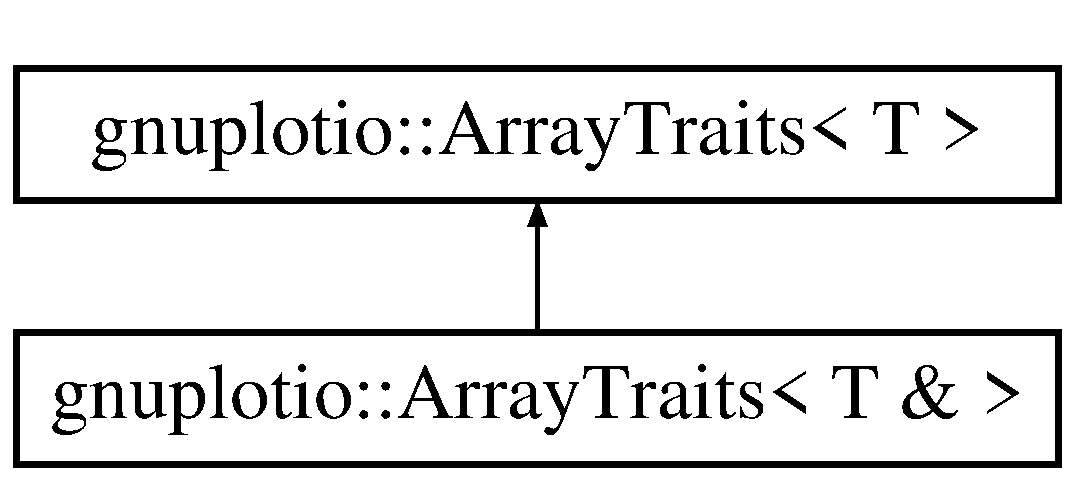
\includegraphics[height=2.000000cm]{classgnuplotio_1_1_array_traits_3_01_t_01_6_01_4}
\end{center}
\end{figure}
\subsection*{Additional Inherited Members}


\subsection{Detailed Description}
\subsubsection*{template$<$typename T$>$\\*
class gnuplotio\+::\+Array\+Traits$<$ T \& $>$}



Definition at line 846 of file gnuplot-\/iostream.\+h.



The documentation for this class was generated from the following file\+:\begin{DoxyCompactItemize}
\item 
include/\hyperlink{gnuplot-iostream_8h}{gnuplot-\/iostream.\+h}\end{DoxyCompactItemize}

\hypertarget{classgnuplotio_1_1_array_traits_3_01_t_00_01typename_01boost_1_1enable__if_3_01boost_1_1mpl_1_1a8de3a8fe198d85f7f5d28b9a2f5bf229}{}\section{gnuplotio\+:\+:Array\+Traits$<$ T, typename boost\+:\+:enable\+\_\+if$<$ boost\+:\+:mpl\+:\+:and\+\_\+$<$ is\+\_\+boost\+\_\+tuple$<$ T $>$, boost\+:\+:mpl\+:\+:not\+\_\+$<$ is\+\_\+boost\+\_\+tuple\+\_\+nulltype$<$ typename T\+:\+:tail\+\_\+type $>$ $>$ $>$ $>$\+:\+:type $>$ Class Template Reference}
\label{classgnuplotio_1_1_array_traits_3_01_t_00_01typename_01boost_1_1enable__if_3_01boost_1_1mpl_1_1a8de3a8fe198d85f7f5d28b9a2f5bf229}\index{gnuplotio\+::\+Array\+Traits$<$ T, typename boost\+::enable\+\_\+if$<$ boost\+::mpl\+::and\+\_\+$<$ is\+\_\+boost\+\_\+tuple$<$ T $>$, boost\+::mpl\+::not\+\_\+$<$ is\+\_\+boost\+\_\+tuple\+\_\+nulltype$<$ typename T\+::tail\+\_\+type $>$ $>$ $>$ $>$\+::type $>$@{gnuplotio\+::\+Array\+Traits$<$ T, typename boost\+::enable\+\_\+if$<$ boost\+::mpl\+::and\+\_\+$<$ is\+\_\+boost\+\_\+tuple$<$ T $>$, boost\+::mpl\+::not\+\_\+$<$ is\+\_\+boost\+\_\+tuple\+\_\+nulltype$<$ typename T\+::tail\+\_\+type $>$ $>$ $>$ $>$\+::type $>$}}


{\ttfamily \#include $<$gnuplot-\/iostream.\+h$>$}

Inheritance diagram for gnuplotio\+:\+:Array\+Traits$<$ T, typename boost\+:\+:enable\+\_\+if$<$ boost\+:\+:mpl\+:\+:and\+\_\+$<$ is\+\_\+boost\+\_\+tuple$<$ T $>$, boost\+:\+:mpl\+:\+:not\+\_\+$<$ is\+\_\+boost\+\_\+tuple\+\_\+nulltype$<$ typename T\+:\+:tail\+\_\+type $>$ $>$ $>$ $>$\+:\+:type $>$\+:\begin{figure}[H]
\begin{center}
\leavevmode
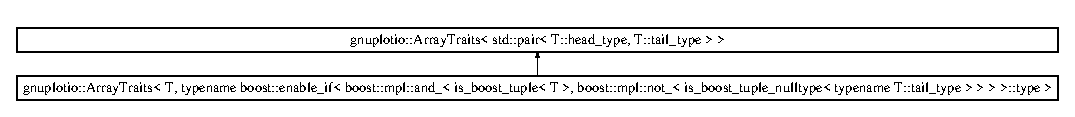
\includegraphics[height=1.122244cm]{classgnuplotio_1_1_array_traits_3_01_t_00_01typename_01boost_1_1enable__if_3_01boost_1_1mpl_1_1a8de3a8fe198d85f7f5d28b9a2f5bf229}
\end{center}
\end{figure}
\subsection*{Public Types}
\begin{DoxyCompactItemize}
\item 
typedef T\+::head\+\_\+type \hyperlink{classgnuplotio_1_1_array_traits_3_01_t_00_01typename_01boost_1_1enable__if_3_01boost_1_1mpl_1_1a8de3a8fe198d85f7f5d28b9a2f5bf229_ab56761f05b74be318cc7becbc59348df}{HT}
\item 
typedef T\+::tail\+\_\+type \hyperlink{classgnuplotio_1_1_array_traits_3_01_t_00_01typename_01boost_1_1enable__if_3_01boost_1_1mpl_1_1a8de3a8fe198d85f7f5d28b9a2f5bf229_a16316f598ab57b0b7ceea99dcd34632e}{TT}
\item 
typedef \hyperlink{classgnuplotio_1_1_array_traits}{Array\+Traits}$<$ typename std\+::pair$<$ \hyperlink{classgnuplotio_1_1_array_traits_3_01_t_00_01typename_01boost_1_1enable__if_3_01boost_1_1mpl_1_1a8de3a8fe198d85f7f5d28b9a2f5bf229_ab56761f05b74be318cc7becbc59348df}{HT}, \hyperlink{classgnuplotio_1_1_array_traits_3_01_t_00_01typename_01boost_1_1enable__if_3_01boost_1_1mpl_1_1a8de3a8fe198d85f7f5d28b9a2f5bf229_a16316f598ab57b0b7ceea99dcd34632e}{TT} $>$ $>$ \hyperlink{classgnuplotio_1_1_array_traits_3_01_t_00_01typename_01boost_1_1enable__if_3_01boost_1_1mpl_1_1a8de3a8fe198d85f7f5d28b9a2f5bf229_aad44f59a1d618b863442a9fdaa83d142}{parent}
\end{DoxyCompactItemize}
\subsection*{Static Public Member Functions}
\begin{DoxyCompactItemize}
\item 
static \hyperlink{classgnuplotio_1_1_array_traits_ae53464a5175c03deec403392b8dcb3c5}{parent\+::range\+\_\+type} \hyperlink{classgnuplotio_1_1_array_traits_3_01_t_00_01typename_01boost_1_1enable__if_3_01boost_1_1mpl_1_1a8de3a8fe198d85f7f5d28b9a2f5bf229_aec07e01edbb46f5f283d5b6af068c0f2}{get\+\_\+range} (const T \&arg)
\end{DoxyCompactItemize}
\subsection*{Additional Inherited Members}


\subsection{Detailed Description}
\subsubsection*{template$<$typename T$>$\\*
class gnuplotio\+::\+Array\+Traits$<$ T, typename boost\+::enable\+\_\+if$<$ boost\+::mpl\+::and\+\_\+$<$ is\+\_\+boost\+\_\+tuple$<$ T $>$, boost\+::mpl\+::not\+\_\+$<$ is\+\_\+boost\+\_\+tuple\+\_\+nulltype$<$ typename T\+::tail\+\_\+type $>$ $>$ $>$ $>$\+::type $>$}



Definition at line 994 of file gnuplot-\/iostream.\+h.



\subsection{Member Typedef Documentation}
\index{gnuplotio\+::\+Array\+Traits$<$ T, typename boost\+::enable\+\_\+if$<$ boost\+::mpl\+::and\+\_\+$<$ is\+\_\+boost\+\_\+tuple$<$ T $>$, boost\+::mpl\+::not\+\_\+$<$ is\+\_\+boost\+\_\+tuple\+\_\+nulltype$<$ typename T\+::tail\+\_\+type $>$ $>$ $>$ $>$\+::type $>$@{gnuplotio\+::\+Array\+Traits$<$ T, typename boost\+::enable\+\_\+if$<$ boost\+::mpl\+::and\+\_\+$<$ is\+\_\+boost\+\_\+tuple$<$ T $>$, boost\+::mpl\+::not\+\_\+$<$ is\+\_\+boost\+\_\+tuple\+\_\+nulltype$<$ typename T\+::tail\+\_\+type $>$ $>$ $>$ $>$\+::type $>$}!HT@{HT}}
\index{HT@{HT}!gnuplotio\+::\+Array\+Traits$<$ T, typename boost\+::enable\+\_\+if$<$ boost\+::mpl\+::and\+\_\+$<$ is\+\_\+boost\+\_\+tuple$<$ T $>$, boost\+::mpl\+::not\+\_\+$<$ is\+\_\+boost\+\_\+tuple\+\_\+nulltype$<$ typename T\+::tail\+\_\+type $>$ $>$ $>$ $>$\+::type $>$@{gnuplotio\+::\+Array\+Traits$<$ T, typename boost\+::enable\+\_\+if$<$ boost\+::mpl\+::and\+\_\+$<$ is\+\_\+boost\+\_\+tuple$<$ T $>$, boost\+::mpl\+::not\+\_\+$<$ is\+\_\+boost\+\_\+tuple\+\_\+nulltype$<$ typename T\+::tail\+\_\+type $>$ $>$ $>$ $>$\+::type $>$}}
\subsubsection[{\texorpdfstring{HT}{HT}}]{\setlength{\rightskip}{0pt plus 5cm}template$<$typename T $>$ typedef T\+::head\+\_\+type {\bf gnuplotio\+::\+Array\+Traits}$<$ T, typename boost\+::enable\+\_\+if$<$ boost\+::mpl\+::and\+\_\+$<$ {\bf is\+\_\+boost\+\_\+tuple}$<$ T $>$, boost\+::mpl\+::not\+\_\+$<$ {\bf is\+\_\+boost\+\_\+tuple\+\_\+nulltype}$<$ typename T\+::tail\+\_\+type $>$ $>$ $>$ $>$\+::type $>$\+::{\bf HT}}\hypertarget{classgnuplotio_1_1_array_traits_3_01_t_00_01typename_01boost_1_1enable__if_3_01boost_1_1mpl_1_1a8de3a8fe198d85f7f5d28b9a2f5bf229_ab56761f05b74be318cc7becbc59348df}{}\label{classgnuplotio_1_1_array_traits_3_01_t_00_01typename_01boost_1_1enable__if_3_01boost_1_1mpl_1_1a8de3a8fe198d85f7f5d28b9a2f5bf229_ab56761f05b74be318cc7becbc59348df}


Definition at line 1008 of file gnuplot-\/iostream.\+h.

\index{gnuplotio\+::\+Array\+Traits$<$ T, typename boost\+::enable\+\_\+if$<$ boost\+::mpl\+::and\+\_\+$<$ is\+\_\+boost\+\_\+tuple$<$ T $>$, boost\+::mpl\+::not\+\_\+$<$ is\+\_\+boost\+\_\+tuple\+\_\+nulltype$<$ typename T\+::tail\+\_\+type $>$ $>$ $>$ $>$\+::type $>$@{gnuplotio\+::\+Array\+Traits$<$ T, typename boost\+::enable\+\_\+if$<$ boost\+::mpl\+::and\+\_\+$<$ is\+\_\+boost\+\_\+tuple$<$ T $>$, boost\+::mpl\+::not\+\_\+$<$ is\+\_\+boost\+\_\+tuple\+\_\+nulltype$<$ typename T\+::tail\+\_\+type $>$ $>$ $>$ $>$\+::type $>$}!parent@{parent}}
\index{parent@{parent}!gnuplotio\+::\+Array\+Traits$<$ T, typename boost\+::enable\+\_\+if$<$ boost\+::mpl\+::and\+\_\+$<$ is\+\_\+boost\+\_\+tuple$<$ T $>$, boost\+::mpl\+::not\+\_\+$<$ is\+\_\+boost\+\_\+tuple\+\_\+nulltype$<$ typename T\+::tail\+\_\+type $>$ $>$ $>$ $>$\+::type $>$@{gnuplotio\+::\+Array\+Traits$<$ T, typename boost\+::enable\+\_\+if$<$ boost\+::mpl\+::and\+\_\+$<$ is\+\_\+boost\+\_\+tuple$<$ T $>$, boost\+::mpl\+::not\+\_\+$<$ is\+\_\+boost\+\_\+tuple\+\_\+nulltype$<$ typename T\+::tail\+\_\+type $>$ $>$ $>$ $>$\+::type $>$}}
\subsubsection[{\texorpdfstring{parent}{parent}}]{\setlength{\rightskip}{0pt plus 5cm}template$<$typename T $>$ typedef {\bf Array\+Traits}$<$typename std\+::pair$<${\bf HT}, {\bf TT}$>$ $>$ {\bf gnuplotio\+::\+Array\+Traits}$<$ T, typename boost\+::enable\+\_\+if$<$ boost\+::mpl\+::and\+\_\+$<$ {\bf is\+\_\+boost\+\_\+tuple}$<$ T $>$, boost\+::mpl\+::not\+\_\+$<$ {\bf is\+\_\+boost\+\_\+tuple\+\_\+nulltype}$<$ typename T\+::tail\+\_\+type $>$ $>$ $>$ $>$\+::type $>$\+::{\bf parent}}\hypertarget{classgnuplotio_1_1_array_traits_3_01_t_00_01typename_01boost_1_1enable__if_3_01boost_1_1mpl_1_1a8de3a8fe198d85f7f5d28b9a2f5bf229_aad44f59a1d618b863442a9fdaa83d142}{}\label{classgnuplotio_1_1_array_traits_3_01_t_00_01typename_01boost_1_1enable__if_3_01boost_1_1mpl_1_1a8de3a8fe198d85f7f5d28b9a2f5bf229_aad44f59a1d618b863442a9fdaa83d142}


Definition at line 1011 of file gnuplot-\/iostream.\+h.

\index{gnuplotio\+::\+Array\+Traits$<$ T, typename boost\+::enable\+\_\+if$<$ boost\+::mpl\+::and\+\_\+$<$ is\+\_\+boost\+\_\+tuple$<$ T $>$, boost\+::mpl\+::not\+\_\+$<$ is\+\_\+boost\+\_\+tuple\+\_\+nulltype$<$ typename T\+::tail\+\_\+type $>$ $>$ $>$ $>$\+::type $>$@{gnuplotio\+::\+Array\+Traits$<$ T, typename boost\+::enable\+\_\+if$<$ boost\+::mpl\+::and\+\_\+$<$ is\+\_\+boost\+\_\+tuple$<$ T $>$, boost\+::mpl\+::not\+\_\+$<$ is\+\_\+boost\+\_\+tuple\+\_\+nulltype$<$ typename T\+::tail\+\_\+type $>$ $>$ $>$ $>$\+::type $>$}!TT@{TT}}
\index{TT@{TT}!gnuplotio\+::\+Array\+Traits$<$ T, typename boost\+::enable\+\_\+if$<$ boost\+::mpl\+::and\+\_\+$<$ is\+\_\+boost\+\_\+tuple$<$ T $>$, boost\+::mpl\+::not\+\_\+$<$ is\+\_\+boost\+\_\+tuple\+\_\+nulltype$<$ typename T\+::tail\+\_\+type $>$ $>$ $>$ $>$\+::type $>$@{gnuplotio\+::\+Array\+Traits$<$ T, typename boost\+::enable\+\_\+if$<$ boost\+::mpl\+::and\+\_\+$<$ is\+\_\+boost\+\_\+tuple$<$ T $>$, boost\+::mpl\+::not\+\_\+$<$ is\+\_\+boost\+\_\+tuple\+\_\+nulltype$<$ typename T\+::tail\+\_\+type $>$ $>$ $>$ $>$\+::type $>$}}
\subsubsection[{\texorpdfstring{TT}{TT}}]{\setlength{\rightskip}{0pt plus 5cm}template$<$typename T $>$ typedef T\+::tail\+\_\+type {\bf gnuplotio\+::\+Array\+Traits}$<$ T, typename boost\+::enable\+\_\+if$<$ boost\+::mpl\+::and\+\_\+$<$ {\bf is\+\_\+boost\+\_\+tuple}$<$ T $>$, boost\+::mpl\+::not\+\_\+$<$ {\bf is\+\_\+boost\+\_\+tuple\+\_\+nulltype}$<$ typename T\+::tail\+\_\+type $>$ $>$ $>$ $>$\+::type $>$\+::{\bf TT}}\hypertarget{classgnuplotio_1_1_array_traits_3_01_t_00_01typename_01boost_1_1enable__if_3_01boost_1_1mpl_1_1a8de3a8fe198d85f7f5d28b9a2f5bf229_a16316f598ab57b0b7ceea99dcd34632e}{}\label{classgnuplotio_1_1_array_traits_3_01_t_00_01typename_01boost_1_1enable__if_3_01boost_1_1mpl_1_1a8de3a8fe198d85f7f5d28b9a2f5bf229_a16316f598ab57b0b7ceea99dcd34632e}


Definition at line 1009 of file gnuplot-\/iostream.\+h.



\subsection{Member Function Documentation}
\index{gnuplotio\+::\+Array\+Traits$<$ T, typename boost\+::enable\+\_\+if$<$ boost\+::mpl\+::and\+\_\+$<$ is\+\_\+boost\+\_\+tuple$<$ T $>$, boost\+::mpl\+::not\+\_\+$<$ is\+\_\+boost\+\_\+tuple\+\_\+nulltype$<$ typename T\+::tail\+\_\+type $>$ $>$ $>$ $>$\+::type $>$@{gnuplotio\+::\+Array\+Traits$<$ T, typename boost\+::enable\+\_\+if$<$ boost\+::mpl\+::and\+\_\+$<$ is\+\_\+boost\+\_\+tuple$<$ T $>$, boost\+::mpl\+::not\+\_\+$<$ is\+\_\+boost\+\_\+tuple\+\_\+nulltype$<$ typename T\+::tail\+\_\+type $>$ $>$ $>$ $>$\+::type $>$}!get\+\_\+range@{get\+\_\+range}}
\index{get\+\_\+range@{get\+\_\+range}!gnuplotio\+::\+Array\+Traits$<$ T, typename boost\+::enable\+\_\+if$<$ boost\+::mpl\+::and\+\_\+$<$ is\+\_\+boost\+\_\+tuple$<$ T $>$, boost\+::mpl\+::not\+\_\+$<$ is\+\_\+boost\+\_\+tuple\+\_\+nulltype$<$ typename T\+::tail\+\_\+type $>$ $>$ $>$ $>$\+::type $>$@{gnuplotio\+::\+Array\+Traits$<$ T, typename boost\+::enable\+\_\+if$<$ boost\+::mpl\+::and\+\_\+$<$ is\+\_\+boost\+\_\+tuple$<$ T $>$, boost\+::mpl\+::not\+\_\+$<$ is\+\_\+boost\+\_\+tuple\+\_\+nulltype$<$ typename T\+::tail\+\_\+type $>$ $>$ $>$ $>$\+::type $>$}}
\subsubsection[{\texorpdfstring{get\+\_\+range(const T \&arg)}{get_range(const T &arg)}}]{\setlength{\rightskip}{0pt plus 5cm}template$<$typename T $>$ static {\bf parent\+::range\+\_\+type} {\bf gnuplotio\+::\+Array\+Traits}$<$ T, typename boost\+::enable\+\_\+if$<$ boost\+::mpl\+::and\+\_\+$<$ {\bf is\+\_\+boost\+\_\+tuple}$<$ T $>$, boost\+::mpl\+::not\+\_\+$<$ {\bf is\+\_\+boost\+\_\+tuple\+\_\+nulltype}$<$ typename T\+::tail\+\_\+type $>$ $>$ $>$ $>$\+::type $>$\+::get\+\_\+range (
\begin{DoxyParamCaption}
\item[{const T \&}]{arg}
\end{DoxyParamCaption}
)\hspace{0.3cm}{\ttfamily [inline]}, {\ttfamily [static]}}\hypertarget{classgnuplotio_1_1_array_traits_3_01_t_00_01typename_01boost_1_1enable__if_3_01boost_1_1mpl_1_1a8de3a8fe198d85f7f5d28b9a2f5bf229_aec07e01edbb46f5f283d5b6af068c0f2}{}\label{classgnuplotio_1_1_array_traits_3_01_t_00_01typename_01boost_1_1enable__if_3_01boost_1_1mpl_1_1a8de3a8fe198d85f7f5d28b9a2f5bf229_aec07e01edbb46f5f283d5b6af068c0f2}


Definition at line 1013 of file gnuplot-\/iostream.\+h.



The documentation for this class was generated from the following file\+:\begin{DoxyCompactItemize}
\item 
include/\hyperlink{gnuplot-iostream_8h}{gnuplot-\/iostream.\+h}\end{DoxyCompactItemize}

\hypertarget{classgnuplotio_1_1_array_traits_3_01_t_00_01typename_01boost_1_1enable__if_3_01boost_1_1mpl_1_1ad3fa8e75dccbaae12a06d17831678a88}{}\section{gnuplotio\+:\+:Array\+Traits$<$ T, typename boost\+:\+:enable\+\_\+if$<$ boost\+:\+:mpl\+:\+:and\+\_\+$<$ is\+\_\+boost\+\_\+tuple$<$ T $>$, is\+\_\+boost\+\_\+tuple\+\_\+nulltype$<$ typename T\+:\+:tail\+\_\+type $>$ $>$ $>$\+:\+:type $>$ Class Template Reference}
\label{classgnuplotio_1_1_array_traits_3_01_t_00_01typename_01boost_1_1enable__if_3_01boost_1_1mpl_1_1ad3fa8e75dccbaae12a06d17831678a88}\index{gnuplotio\+::\+Array\+Traits$<$ T, typename boost\+::enable\+\_\+if$<$ boost\+::mpl\+::and\+\_\+$<$ is\+\_\+boost\+\_\+tuple$<$ T $>$, is\+\_\+boost\+\_\+tuple\+\_\+nulltype$<$ typename T\+::tail\+\_\+type $>$ $>$ $>$\+::type $>$@{gnuplotio\+::\+Array\+Traits$<$ T, typename boost\+::enable\+\_\+if$<$ boost\+::mpl\+::and\+\_\+$<$ is\+\_\+boost\+\_\+tuple$<$ T $>$, is\+\_\+boost\+\_\+tuple\+\_\+nulltype$<$ typename T\+::tail\+\_\+type $>$ $>$ $>$\+::type $>$}}


{\ttfamily \#include $<$gnuplot-\/iostream.\+h$>$}

Inheritance diagram for gnuplotio\+:\+:Array\+Traits$<$ T, typename boost\+:\+:enable\+\_\+if$<$ boost\+:\+:mpl\+:\+:and\+\_\+$<$ is\+\_\+boost\+\_\+tuple$<$ T $>$, is\+\_\+boost\+\_\+tuple\+\_\+nulltype$<$ typename T\+:\+:tail\+\_\+type $>$ $>$ $>$\+:\+:type $>$\+:\begin{figure}[H]
\begin{center}
\leavevmode
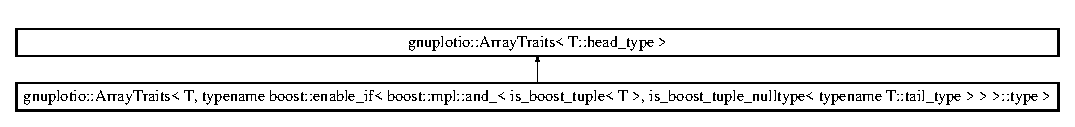
\includegraphics[height=1.259843cm]{classgnuplotio_1_1_array_traits_3_01_t_00_01typename_01boost_1_1enable__if_3_01boost_1_1mpl_1_1ad3fa8e75dccbaae12a06d17831678a88}
\end{center}
\end{figure}
\subsection*{Static Public Member Functions}
\begin{DoxyCompactItemize}
\item 
static \hyperlink{classgnuplotio_1_1_array_traits_ae53464a5175c03deec403392b8dcb3c5}{parent\+::range\+\_\+type} \hyperlink{classgnuplotio_1_1_array_traits_3_01_t_00_01typename_01boost_1_1enable__if_3_01boost_1_1mpl_1_1ad3fa8e75dccbaae12a06d17831678a88_ad0485dd16a9d54a4eb75bf3e75b1facd}{get\+\_\+range} (const T \&arg)
\end{DoxyCompactItemize}
\subsection*{Additional Inherited Members}


\subsection{Detailed Description}
\subsubsection*{template$<$typename T$>$\\*
class gnuplotio\+::\+Array\+Traits$<$ T, typename boost\+::enable\+\_\+if$<$ boost\+::mpl\+::and\+\_\+$<$ is\+\_\+boost\+\_\+tuple$<$ T $>$, is\+\_\+boost\+\_\+tuple\+\_\+nulltype$<$ typename T\+::tail\+\_\+type $>$ $>$ $>$\+::type $>$}



Definition at line 1022 of file gnuplot-\/iostream.\+h.



\subsection{Member Function Documentation}
\index{gnuplotio\+::\+Array\+Traits$<$ T, typename boost\+::enable\+\_\+if$<$ boost\+::mpl\+::and\+\_\+$<$ is\+\_\+boost\+\_\+tuple$<$ T $>$, is\+\_\+boost\+\_\+tuple\+\_\+nulltype$<$ typename T\+::tail\+\_\+type $>$ $>$ $>$\+::type $>$@{gnuplotio\+::\+Array\+Traits$<$ T, typename boost\+::enable\+\_\+if$<$ boost\+::mpl\+::and\+\_\+$<$ is\+\_\+boost\+\_\+tuple$<$ T $>$, is\+\_\+boost\+\_\+tuple\+\_\+nulltype$<$ typename T\+::tail\+\_\+type $>$ $>$ $>$\+::type $>$}!get\+\_\+range@{get\+\_\+range}}
\index{get\+\_\+range@{get\+\_\+range}!gnuplotio\+::\+Array\+Traits$<$ T, typename boost\+::enable\+\_\+if$<$ boost\+::mpl\+::and\+\_\+$<$ is\+\_\+boost\+\_\+tuple$<$ T $>$, is\+\_\+boost\+\_\+tuple\+\_\+nulltype$<$ typename T\+::tail\+\_\+type $>$ $>$ $>$\+::type $>$@{gnuplotio\+::\+Array\+Traits$<$ T, typename boost\+::enable\+\_\+if$<$ boost\+::mpl\+::and\+\_\+$<$ is\+\_\+boost\+\_\+tuple$<$ T $>$, is\+\_\+boost\+\_\+tuple\+\_\+nulltype$<$ typename T\+::tail\+\_\+type $>$ $>$ $>$\+::type $>$}}
\subsubsection[{\texorpdfstring{get\+\_\+range(const T \&arg)}{get_range(const T &arg)}}]{\setlength{\rightskip}{0pt plus 5cm}template$<$typename T $>$ static {\bf parent\+::range\+\_\+type} {\bf gnuplotio\+::\+Array\+Traits}$<$ T, typename boost\+::enable\+\_\+if$<$ boost\+::mpl\+::and\+\_\+$<$ {\bf is\+\_\+boost\+\_\+tuple}$<$ T $>$, {\bf is\+\_\+boost\+\_\+tuple\+\_\+nulltype}$<$ typename T\+::tail\+\_\+type $>$ $>$ $>$\+::type $>$\+::get\+\_\+range (
\begin{DoxyParamCaption}
\item[{const T \&}]{arg}
\end{DoxyParamCaption}
)\hspace{0.3cm}{\ttfamily [inline]}, {\ttfamily [static]}}\hypertarget{classgnuplotio_1_1_array_traits_3_01_t_00_01typename_01boost_1_1enable__if_3_01boost_1_1mpl_1_1ad3fa8e75dccbaae12a06d17831678a88_ad0485dd16a9d54a4eb75bf3e75b1facd}{}\label{classgnuplotio_1_1_array_traits_3_01_t_00_01typename_01boost_1_1enable__if_3_01boost_1_1mpl_1_1ad3fa8e75dccbaae12a06d17831678a88_ad0485dd16a9d54a4eb75bf3e75b1facd}


Definition at line 1037 of file gnuplot-\/iostream.\+h.



The documentation for this class was generated from the following file\+:\begin{DoxyCompactItemize}
\item 
include/\hyperlink{gnuplot-iostream_8h}{gnuplot-\/iostream.\+h}\end{DoxyCompactItemize}

\hypertarget{classgnuplotio_1_1_array_traits_3_01_t_00_01typename_01boost_1_1enable__if_3_01is__like__stl__co9e1736bbd08cd58c6993ab613a998887}{}\section{gnuplotio\+:\+:Array\+Traits$<$ T, typename boost\+:\+:enable\+\_\+if$<$ is\+\_\+like\+\_\+stl\+\_\+container$<$ T $>$ $>$\+:\+:type $>$ Class Template Reference}
\label{classgnuplotio_1_1_array_traits_3_01_t_00_01typename_01boost_1_1enable__if_3_01is__like__stl__co9e1736bbd08cd58c6993ab613a998887}\index{gnuplotio\+::\+Array\+Traits$<$ T, typename boost\+::enable\+\_\+if$<$ is\+\_\+like\+\_\+stl\+\_\+container$<$ T $>$ $>$\+::type $>$@{gnuplotio\+::\+Array\+Traits$<$ T, typename boost\+::enable\+\_\+if$<$ is\+\_\+like\+\_\+stl\+\_\+container$<$ T $>$ $>$\+::type $>$}}


{\ttfamily \#include $<$gnuplot-\/iostream.\+h$>$}

Inheritance diagram for gnuplotio\+:\+:Array\+Traits$<$ T, typename boost\+:\+:enable\+\_\+if$<$ is\+\_\+like\+\_\+stl\+\_\+container$<$ T $>$ $>$\+:\+:type $>$\+:\begin{figure}[H]
\begin{center}
\leavevmode
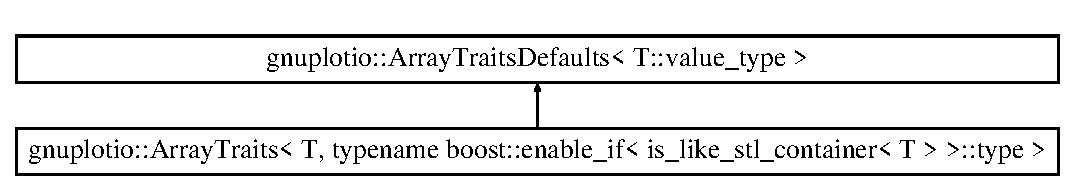
\includegraphics[height=2.000000cm]{classgnuplotio_1_1_array_traits_3_01_t_00_01typename_01boost_1_1enable__if_3_01is__like__stl__co9e1736bbd08cd58c6993ab613a998887}
\end{center}
\end{figure}
\subsection*{Public Types}
\begin{DoxyCompactItemize}
\item 
typedef \hyperlink{classgnuplotio_1_1_iterator_range}{Iterator\+Range}$<$ typename T\+::const\+\_\+iterator, typename \hyperlink{classgnuplotio_1_1_array_traits_a3bcae12a7bf42af90f4946acc66f27e0}{T\+::value\+\_\+type} $>$ \hyperlink{classgnuplotio_1_1_array_traits_3_01_t_00_01typename_01boost_1_1enable__if_3_01is__like__stl__co9e1736bbd08cd58c6993ab613a998887_ab702072abbe018bbc90b9967ca8c4b42}{range\+\_\+type}
\end{DoxyCompactItemize}
\subsection*{Static Public Member Functions}
\begin{DoxyCompactItemize}
\item 
static \hyperlink{classgnuplotio_1_1_array_traits_3_01_t_00_01typename_01boost_1_1enable__if_3_01is__like__stl__co9e1736bbd08cd58c6993ab613a998887_ab702072abbe018bbc90b9967ca8c4b42}{range\+\_\+type} \hyperlink{classgnuplotio_1_1_array_traits_3_01_t_00_01typename_01boost_1_1enable__if_3_01is__like__stl__co9e1736bbd08cd58c6993ab613a998887_a89d4150ab3c479cde972071a10acd27b}{get\+\_\+range} (const T \&arg)
\end{DoxyCompactItemize}
\subsection*{Additional Inherited Members}


\subsection{Detailed Description}
\subsubsection*{template$<$typename T$>$\\*
class gnuplotio\+::\+Array\+Traits$<$ T, typename boost\+::enable\+\_\+if$<$ is\+\_\+like\+\_\+stl\+\_\+container$<$ T $>$ $>$\+::type $>$}



Definition at line 897 of file gnuplot-\/iostream.\+h.



\subsection{Member Typedef Documentation}
\index{gnuplotio\+::\+Array\+Traits$<$ T, typename boost\+::enable\+\_\+if$<$ is\+\_\+like\+\_\+stl\+\_\+container$<$ T $>$ $>$\+::type $>$@{gnuplotio\+::\+Array\+Traits$<$ T, typename boost\+::enable\+\_\+if$<$ is\+\_\+like\+\_\+stl\+\_\+container$<$ T $>$ $>$\+::type $>$}!range\+\_\+type@{range\+\_\+type}}
\index{range\+\_\+type@{range\+\_\+type}!gnuplotio\+::\+Array\+Traits$<$ T, typename boost\+::enable\+\_\+if$<$ is\+\_\+like\+\_\+stl\+\_\+container$<$ T $>$ $>$\+::type $>$@{gnuplotio\+::\+Array\+Traits$<$ T, typename boost\+::enable\+\_\+if$<$ is\+\_\+like\+\_\+stl\+\_\+container$<$ T $>$ $>$\+::type $>$}}
\subsubsection[{\texorpdfstring{range\+\_\+type}{range_type}}]{\setlength{\rightskip}{0pt plus 5cm}template$<$typename T $>$ typedef {\bf Iterator\+Range}$<$typename T\+::const\+\_\+iterator, typename {\bf T\+::value\+\_\+type}$>$ {\bf gnuplotio\+::\+Array\+Traits}$<$ T, typename boost\+::enable\+\_\+if$<$ {\bf is\+\_\+like\+\_\+stl\+\_\+container}$<$ T $>$ $>$\+::type $>$\+::{\bf range\+\_\+type}}\hypertarget{classgnuplotio_1_1_array_traits_3_01_t_00_01typename_01boost_1_1enable__if_3_01is__like__stl__co9e1736bbd08cd58c6993ab613a998887_ab702072abbe018bbc90b9967ca8c4b42}{}\label{classgnuplotio_1_1_array_traits_3_01_t_00_01typename_01boost_1_1enable__if_3_01is__like__stl__co9e1736bbd08cd58c6993ab613a998887_ab702072abbe018bbc90b9967ca8c4b42}


Definition at line 901 of file gnuplot-\/iostream.\+h.



\subsection{Member Function Documentation}
\index{gnuplotio\+::\+Array\+Traits$<$ T, typename boost\+::enable\+\_\+if$<$ is\+\_\+like\+\_\+stl\+\_\+container$<$ T $>$ $>$\+::type $>$@{gnuplotio\+::\+Array\+Traits$<$ T, typename boost\+::enable\+\_\+if$<$ is\+\_\+like\+\_\+stl\+\_\+container$<$ T $>$ $>$\+::type $>$}!get\+\_\+range@{get\+\_\+range}}
\index{get\+\_\+range@{get\+\_\+range}!gnuplotio\+::\+Array\+Traits$<$ T, typename boost\+::enable\+\_\+if$<$ is\+\_\+like\+\_\+stl\+\_\+container$<$ T $>$ $>$\+::type $>$@{gnuplotio\+::\+Array\+Traits$<$ T, typename boost\+::enable\+\_\+if$<$ is\+\_\+like\+\_\+stl\+\_\+container$<$ T $>$ $>$\+::type $>$}}
\subsubsection[{\texorpdfstring{get\+\_\+range(const T \&arg)}{get_range(const T &arg)}}]{\setlength{\rightskip}{0pt plus 5cm}template$<$typename T $>$ static {\bf range\+\_\+type} {\bf gnuplotio\+::\+Array\+Traits}$<$ T, typename boost\+::enable\+\_\+if$<$ {\bf is\+\_\+like\+\_\+stl\+\_\+container}$<$ T $>$ $>$\+::type $>$\+::get\+\_\+range (
\begin{DoxyParamCaption}
\item[{const T \&}]{arg}
\end{DoxyParamCaption}
)\hspace{0.3cm}{\ttfamily [inline]}, {\ttfamily [static]}}\hypertarget{classgnuplotio_1_1_array_traits_3_01_t_00_01typename_01boost_1_1enable__if_3_01is__like__stl__co9e1736bbd08cd58c6993ab613a998887_a89d4150ab3c479cde972071a10acd27b}{}\label{classgnuplotio_1_1_array_traits_3_01_t_00_01typename_01boost_1_1enable__if_3_01is__like__stl__co9e1736bbd08cd58c6993ab613a998887_a89d4150ab3c479cde972071a10acd27b}


Definition at line 903 of file gnuplot-\/iostream.\+h.



The documentation for this class was generated from the following file\+:\begin{DoxyCompactItemize}
\item 
include/\hyperlink{gnuplot-iostream_8h}{gnuplot-\/iostream.\+h}\end{DoxyCompactItemize}

\hypertarget{classgnuplotio_1_1_array_traits_3_01_t[_n]_4}{}\section{gnuplotio\+:\+:Array\+Traits$<$ T\mbox{[}N\mbox{]}$>$ Class Template Reference}
\label{classgnuplotio_1_1_array_traits_3_01_t[_n]_4}\index{gnuplotio\+::\+Array\+Traits$<$ T\mbox{[}\+N\mbox{]}$>$@{gnuplotio\+::\+Array\+Traits$<$ T[N]$>$}}


{\ttfamily \#include $<$gnuplot-\/iostream.\+h$>$}

Inheritance diagram for gnuplotio\+:\+:Array\+Traits$<$ T\mbox{[}N\mbox{]}$>$\+:\begin{figure}[H]
\begin{center}
\leavevmode
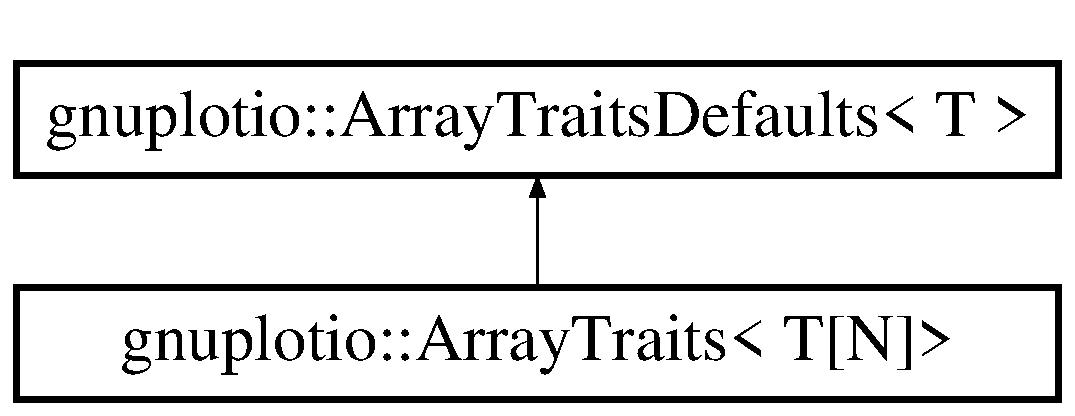
\includegraphics[height=2.000000cm]{classgnuplotio_1_1_array_traits_3_01_t[_n]_4}
\end{center}
\end{figure}
\subsection*{Public Types}
\begin{DoxyCompactItemize}
\item 
typedef \hyperlink{classgnuplotio_1_1_iterator_range}{Iterator\+Range}$<$ const T $\ast$, T $>$ \hyperlink{classgnuplotio_1_1_array_traits_3_01_t[_n]_4_a926f3c3d14fbe82aab7b70ccc16d20fb}{range\+\_\+type}
\end{DoxyCompactItemize}
\subsection*{Static Public Member Functions}
\begin{DoxyCompactItemize}
\item 
static \hyperlink{classgnuplotio_1_1_array_traits_3_01_t[_n]_4_a926f3c3d14fbe82aab7b70ccc16d20fb}{range\+\_\+type} \hyperlink{classgnuplotio_1_1_array_traits_3_01_t[_n]_4_adc9c1ce6da4923418f367e08c150a928}{get\+\_\+range} (const T(\&arg)\mbox{[}N\mbox{]})
\end{DoxyCompactItemize}
\subsection*{Additional Inherited Members}


\subsection{Detailed Description}
\subsubsection*{template$<$typename T, size\+\_\+t N$>$\\*
class gnuplotio\+::\+Array\+Traits$<$ T\mbox{[}\+N\mbox{]}$>$}



Definition at line 913 of file gnuplot-\/iostream.\+h.



\subsection{Member Typedef Documentation}
\index{gnuplotio\+::\+Array\+Traits$<$ T\mbox{[}\+N\mbox{]}$>$@{gnuplotio\+::\+Array\+Traits$<$ T[N]$>$}!range\+\_\+type@{range\+\_\+type}}
\index{range\+\_\+type@{range\+\_\+type}!gnuplotio\+::\+Array\+Traits$<$ T\mbox{[}\+N\mbox{]}$>$@{gnuplotio\+::\+Array\+Traits$<$ T[N]$>$}}
\subsubsection[{\texorpdfstring{range\+\_\+type}{range_type}}]{\setlength{\rightskip}{0pt plus 5cm}template$<$typename T , size\+\_\+t N$>$ typedef {\bf Iterator\+Range}$<$const T$\ast$, T$>$ {\bf gnuplotio\+::\+Array\+Traits}$<$ T\mbox{[}N\mbox{]}$>$\+::{\bf range\+\_\+type}}\hypertarget{classgnuplotio_1_1_array_traits_3_01_t[_n]_4_a926f3c3d14fbe82aab7b70ccc16d20fb}{}\label{classgnuplotio_1_1_array_traits_3_01_t[_n]_4_a926f3c3d14fbe82aab7b70ccc16d20fb}


Definition at line 915 of file gnuplot-\/iostream.\+h.



\subsection{Member Function Documentation}
\index{gnuplotio\+::\+Array\+Traits$<$ T\mbox{[}\+N\mbox{]}$>$@{gnuplotio\+::\+Array\+Traits$<$ T[N]$>$}!get\+\_\+range@{get\+\_\+range}}
\index{get\+\_\+range@{get\+\_\+range}!gnuplotio\+::\+Array\+Traits$<$ T\mbox{[}\+N\mbox{]}$>$@{gnuplotio\+::\+Array\+Traits$<$ T[N]$>$}}
\subsubsection[{\texorpdfstring{get\+\_\+range(const T(\&arg)[N])}{get_range(const T(&arg)[N])}}]{\setlength{\rightskip}{0pt plus 5cm}template$<$typename T , size\+\_\+t N$>$ static {\bf range\+\_\+type} {\bf gnuplotio\+::\+Array\+Traits}$<$ T\mbox{[}N\mbox{]}$>$\+::get\+\_\+range (
\begin{DoxyParamCaption}
\item[{const T(\&)}]{arg\mbox{[}\+N\mbox{]}}
\end{DoxyParamCaption}
)\hspace{0.3cm}{\ttfamily [inline]}, {\ttfamily [static]}}\hypertarget{classgnuplotio_1_1_array_traits_3_01_t[_n]_4_adc9c1ce6da4923418f367e08c150a928}{}\label{classgnuplotio_1_1_array_traits_3_01_t[_n]_4_adc9c1ce6da4923418f367e08c150a928}


Definition at line 917 of file gnuplot-\/iostream.\+h.



The documentation for this class was generated from the following file\+:\begin{DoxyCompactItemize}
\item 
include/\hyperlink{gnuplot-iostream_8h}{gnuplot-\/iostream.\+h}\end{DoxyCompactItemize}

\hypertarget{classgnuplotio_1_1_array_traits_defaults}{}\section{gnuplotio\+:\+:Array\+Traits\+Defaults$<$ V $>$ Class Template Reference}
\label{classgnuplotio_1_1_array_traits_defaults}\index{gnuplotio\+::\+Array\+Traits\+Defaults$<$ V $>$@{gnuplotio\+::\+Array\+Traits\+Defaults$<$ V $>$}}


{\ttfamily \#include $<$gnuplot-\/iostream.\+h$>$}

\subsection*{Public Types}
\begin{DoxyCompactItemize}
\item 
typedef V \hyperlink{classgnuplotio_1_1_array_traits_defaults_ad7a9e8d19419fabe2ab9cc1b76c9965b}{value\+\_\+type}
\end{DoxyCompactItemize}
\subsection*{Static Public Attributes}
\begin{DoxyCompactItemize}
\item 
static const bool \hyperlink{classgnuplotio_1_1_array_traits_defaults_a57bab5bf3617f0ee66fdd4dcb751aa21}{is\+\_\+container} = true
\item 
static const bool \hyperlink{classgnuplotio_1_1_array_traits_defaults_ac8d430cba6ceefc6f52706455f12a0e8}{allow\+\_\+auto\+\_\+unwrap} = true
\item 
static const size\+\_\+t \hyperlink{classgnuplotio_1_1_array_traits_defaults_ac51367f5da9096249b162af1496e36ab}{depth} = \hyperlink{classgnuplotio_1_1_array_traits}{Array\+Traits}$<$V$>$\+::depth + 1
\end{DoxyCompactItemize}


\subsection{Detailed Description}
\subsubsection*{template$<$typename V$>$\\*
class gnuplotio\+::\+Array\+Traits\+Defaults$<$ V $>$}



Definition at line 833 of file gnuplot-\/iostream.\+h.



\subsection{Member Typedef Documentation}
\index{gnuplotio\+::\+Array\+Traits\+Defaults@{gnuplotio\+::\+Array\+Traits\+Defaults}!value\+\_\+type@{value\+\_\+type}}
\index{value\+\_\+type@{value\+\_\+type}!gnuplotio\+::\+Array\+Traits\+Defaults@{gnuplotio\+::\+Array\+Traits\+Defaults}}
\subsubsection[{\texorpdfstring{value\+\_\+type}{value_type}}]{\setlength{\rightskip}{0pt plus 5cm}template$<$typename V$>$ typedef V {\bf gnuplotio\+::\+Array\+Traits\+Defaults}$<$ V $>$\+::{\bf value\+\_\+type}}\hypertarget{classgnuplotio_1_1_array_traits_defaults_ad7a9e8d19419fabe2ab9cc1b76c9965b}{}\label{classgnuplotio_1_1_array_traits_defaults_ad7a9e8d19419fabe2ab9cc1b76c9965b}


Definition at line 835 of file gnuplot-\/iostream.\+h.



\subsection{Member Data Documentation}
\index{gnuplotio\+::\+Array\+Traits\+Defaults@{gnuplotio\+::\+Array\+Traits\+Defaults}!allow\+\_\+auto\+\_\+unwrap@{allow\+\_\+auto\+\_\+unwrap}}
\index{allow\+\_\+auto\+\_\+unwrap@{allow\+\_\+auto\+\_\+unwrap}!gnuplotio\+::\+Array\+Traits\+Defaults@{gnuplotio\+::\+Array\+Traits\+Defaults}}
\subsubsection[{\texorpdfstring{allow\+\_\+auto\+\_\+unwrap}{allow_auto_unwrap}}]{\setlength{\rightskip}{0pt plus 5cm}template$<$typename V$>$ const bool {\bf gnuplotio\+::\+Array\+Traits\+Defaults}$<$ V $>$\+::allow\+\_\+auto\+\_\+unwrap = true\hspace{0.3cm}{\ttfamily [static]}}\hypertarget{classgnuplotio_1_1_array_traits_defaults_ac8d430cba6ceefc6f52706455f12a0e8}{}\label{classgnuplotio_1_1_array_traits_defaults_ac8d430cba6ceefc6f52706455f12a0e8}


Definition at line 838 of file gnuplot-\/iostream.\+h.

\index{gnuplotio\+::\+Array\+Traits\+Defaults@{gnuplotio\+::\+Array\+Traits\+Defaults}!depth@{depth}}
\index{depth@{depth}!gnuplotio\+::\+Array\+Traits\+Defaults@{gnuplotio\+::\+Array\+Traits\+Defaults}}
\subsubsection[{\texorpdfstring{depth}{depth}}]{\setlength{\rightskip}{0pt plus 5cm}template$<$typename V$>$ const size\+\_\+t {\bf gnuplotio\+::\+Array\+Traits\+Defaults}$<$ V $>$\+::depth = {\bf Array\+Traits}$<$V$>$\+::depth + 1\hspace{0.3cm}{\ttfamily [static]}}\hypertarget{classgnuplotio_1_1_array_traits_defaults_ac51367f5da9096249b162af1496e36ab}{}\label{classgnuplotio_1_1_array_traits_defaults_ac51367f5da9096249b162af1496e36ab}


Definition at line 839 of file gnuplot-\/iostream.\+h.

\index{gnuplotio\+::\+Array\+Traits\+Defaults@{gnuplotio\+::\+Array\+Traits\+Defaults}!is\+\_\+container@{is\+\_\+container}}
\index{is\+\_\+container@{is\+\_\+container}!gnuplotio\+::\+Array\+Traits\+Defaults@{gnuplotio\+::\+Array\+Traits\+Defaults}}
\subsubsection[{\texorpdfstring{is\+\_\+container}{is_container}}]{\setlength{\rightskip}{0pt plus 5cm}template$<$typename V$>$ const bool {\bf gnuplotio\+::\+Array\+Traits\+Defaults}$<$ V $>$\+::is\+\_\+container = true\hspace{0.3cm}{\ttfamily [static]}}\hypertarget{classgnuplotio_1_1_array_traits_defaults_a57bab5bf3617f0ee66fdd4dcb751aa21}{}\label{classgnuplotio_1_1_array_traits_defaults_a57bab5bf3617f0ee66fdd4dcb751aa21}


Definition at line 837 of file gnuplot-\/iostream.\+h.



The documentation for this class was generated from the following file\+:\begin{DoxyCompactItemize}
\item 
include/\hyperlink{gnuplot-iostream_8h}{gnuplot-\/iostream.\+h}\end{DoxyCompactItemize}

\hypertarget{structgnuplotio_1_1_binary_sender}{}\section{gnuplotio\+:\+:Binary\+Sender$<$ T, Enable $>$ Struct Template Reference}
\label{structgnuplotio_1_1_binary_sender}\index{gnuplotio\+::\+Binary\+Sender$<$ T, Enable $>$@{gnuplotio\+::\+Binary\+Sender$<$ T, Enable $>$}}


{\ttfamily \#include $<$gnuplot-\/iostream.\+h$>$}

\subsection*{Public Member Functions}
\begin{DoxyCompactItemize}
\item 
\hyperlink{structgnuplotio_1_1_binary_sender_a165c59a28adc4a90930925c6e0bfb0a9}{G\+N\+U\+P\+L\+O\+T\+\_\+\+S\+T\+A\+T\+I\+C\+\_\+\+A\+S\+S\+E\+R\+T\+\_\+\+M\+SG} ((sizeof(T)==0),\char`\"{}Binary\+Sender class not specialized for this type\char`\"{})
\end{DoxyCompactItemize}
\subsection*{Static Public Member Functions}
\begin{DoxyCompactItemize}
\item 
static void \hyperlink{structgnuplotio_1_1_binary_sender_a4b5dd22b7679c4f0ce4d8e75b36c8a21}{send} (std\+::ostream \&stream, const T \&v)
\end{DoxyCompactItemize}


\subsection{Detailed Description}
\subsubsection*{template$<$typename T, typename Enable = void$>$\\*
struct gnuplotio\+::\+Binary\+Sender$<$ T, Enable $>$}



Definition at line 441 of file gnuplot-\/iostream.\+h.



\subsection{Member Function Documentation}
\index{gnuplotio\+::\+Binary\+Sender@{gnuplotio\+::\+Binary\+Sender}!G\+N\+U\+P\+L\+O\+T\+\_\+\+S\+T\+A\+T\+I\+C\+\_\+\+A\+S\+S\+E\+R\+T\+\_\+\+M\+SG@{G\+N\+U\+P\+L\+O\+T\+\_\+\+S\+T\+A\+T\+I\+C\+\_\+\+A\+S\+S\+E\+R\+T\+\_\+\+M\+SG}}
\index{G\+N\+U\+P\+L\+O\+T\+\_\+\+S\+T\+A\+T\+I\+C\+\_\+\+A\+S\+S\+E\+R\+T\+\_\+\+M\+SG@{G\+N\+U\+P\+L\+O\+T\+\_\+\+S\+T\+A\+T\+I\+C\+\_\+\+A\+S\+S\+E\+R\+T\+\_\+\+M\+SG}!gnuplotio\+::\+Binary\+Sender@{gnuplotio\+::\+Binary\+Sender}}
\subsubsection[{\texorpdfstring{G\+N\+U\+P\+L\+O\+T\+\_\+\+S\+T\+A\+T\+I\+C\+\_\+\+A\+S\+S\+E\+R\+T\+\_\+\+M\+S\+G((sizeof(\+T)==0),""Binary\+Sender class not specialized for this type"")}{GNUPLOT_STATIC_ASSERT_MSG((sizeof(T)==0),"BinarySender class not specialized for this type")}}]{\setlength{\rightskip}{0pt plus 5cm}template$<$typename T, typename Enable = void$>$ {\bf gnuplotio\+::\+Binary\+Sender}$<$ T, Enable $>$\+::G\+N\+U\+P\+L\+O\+T\+\_\+\+S\+T\+A\+T\+I\+C\+\_\+\+A\+S\+S\+E\+R\+T\+\_\+\+M\+SG (
\begin{DoxyParamCaption}
\item[{(sizeof(T)==0)}]{, }
\item[{\char`\"{}Binary\+Sender$<$ T, Enable $>$ class not specialized for this type\char`\"{}}]{}
\end{DoxyParamCaption}
)}\hypertarget{structgnuplotio_1_1_binary_sender_a165c59a28adc4a90930925c6e0bfb0a9}{}\label{structgnuplotio_1_1_binary_sender_a165c59a28adc4a90930925c6e0bfb0a9}
\index{gnuplotio\+::\+Binary\+Sender@{gnuplotio\+::\+Binary\+Sender}!send@{send}}
\index{send@{send}!gnuplotio\+::\+Binary\+Sender@{gnuplotio\+::\+Binary\+Sender}}
\subsubsection[{\texorpdfstring{send(std\+::ostream \&stream, const T \&v)}{send(std::ostream &stream, const T &v)}}]{\setlength{\rightskip}{0pt plus 5cm}template$<$typename T, typename Enable = void$>$ static void {\bf gnuplotio\+::\+Binary\+Sender}$<$ T, Enable $>$\+::send (
\begin{DoxyParamCaption}
\item[{std\+::ostream \&}]{stream, }
\item[{const T \&}]{v}
\end{DoxyParamCaption}
)\hspace{0.3cm}{\ttfamily [static]}}\hypertarget{structgnuplotio_1_1_binary_sender_a4b5dd22b7679c4f0ce4d8e75b36c8a21}{}\label{structgnuplotio_1_1_binary_sender_a4b5dd22b7679c4f0ce4d8e75b36c8a21}


The documentation for this struct was generated from the following file\+:\begin{DoxyCompactItemize}
\item 
include/\hyperlink{gnuplot-iostream_8h}{gnuplot-\/iostream.\+h}\end{DoxyCompactItemize}

\hypertarget{structgnuplotio_1_1_binary_sender_3_01boost_1_1int16__t_01_4}{}\section{gnuplotio\+:\+:Binary\+Sender$<$ boost\+:\+:int16\+\_\+t $>$ Struct Template Reference}
\label{structgnuplotio_1_1_binary_sender_3_01boost_1_1int16__t_01_4}\index{gnuplotio\+::\+Binary\+Sender$<$ boost\+::int16\+\_\+t $>$@{gnuplotio\+::\+Binary\+Sender$<$ boost\+::int16\+\_\+t $>$}}


{\ttfamily \#include $<$gnuplot-\/iostream.\+h$>$}

Inheritance diagram for gnuplotio\+:\+:Binary\+Sender$<$ boost\+:\+:int16\+\_\+t $>$\+:\begin{figure}[H]
\begin{center}
\leavevmode
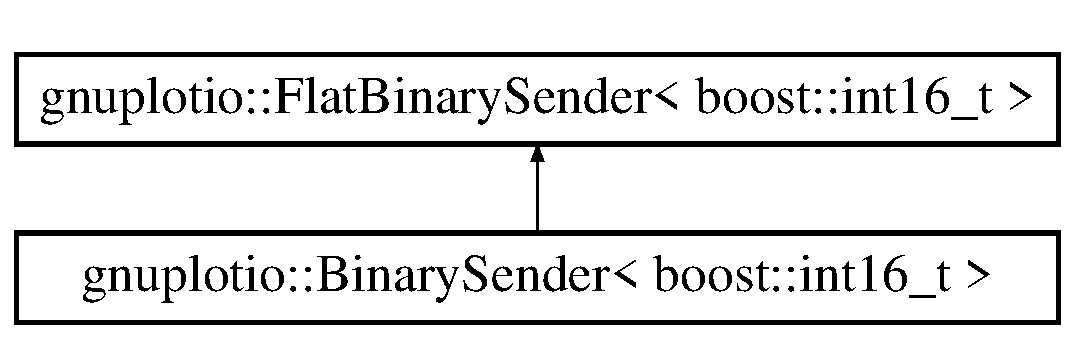
\includegraphics[height=2.000000cm]{structgnuplotio_1_1_binary_sender_3_01boost_1_1int16__t_01_4}
\end{center}
\end{figure}
\subsection*{Additional Inherited Members}


\subsection{Detailed Description}
\subsubsection*{template$<$$>$\\*
struct gnuplotio\+::\+Binary\+Sender$<$ boost\+::int16\+\_\+t $>$}



Definition at line 485 of file gnuplot-\/iostream.\+h.



The documentation for this struct was generated from the following file\+:\begin{DoxyCompactItemize}
\item 
include/\hyperlink{gnuplot-iostream_8h}{gnuplot-\/iostream.\+h}\end{DoxyCompactItemize}

\hypertarget{structgnuplotio_1_1_binary_sender_3_01boost_1_1int32__t_01_4}{}\section{gnuplotio\+:\+:Binary\+Sender$<$ boost\+:\+:int32\+\_\+t $>$ Struct Template Reference}
\label{structgnuplotio_1_1_binary_sender_3_01boost_1_1int32__t_01_4}\index{gnuplotio\+::\+Binary\+Sender$<$ boost\+::int32\+\_\+t $>$@{gnuplotio\+::\+Binary\+Sender$<$ boost\+::int32\+\_\+t $>$}}


{\ttfamily \#include $<$gnuplot-\/iostream.\+h$>$}

Inheritance diagram for gnuplotio\+:\+:Binary\+Sender$<$ boost\+:\+:int32\+\_\+t $>$\+:\begin{figure}[H]
\begin{center}
\leavevmode
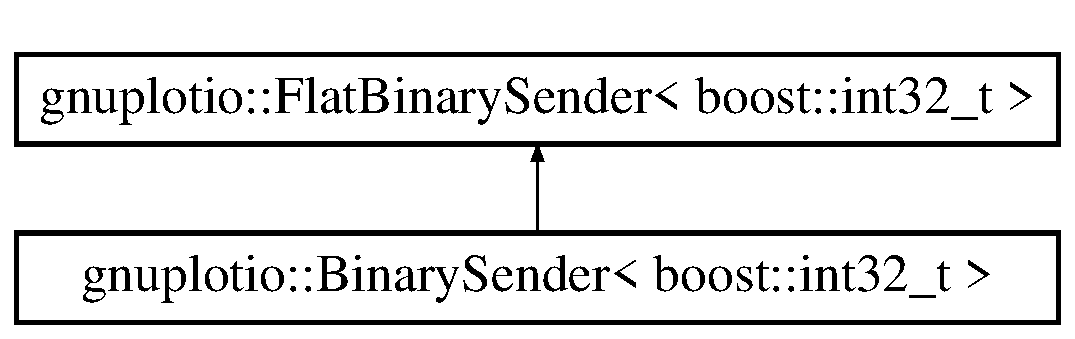
\includegraphics[height=2.000000cm]{structgnuplotio_1_1_binary_sender_3_01boost_1_1int32__t_01_4}
\end{center}
\end{figure}
\subsection*{Additional Inherited Members}


\subsection{Detailed Description}
\subsubsection*{template$<$$>$\\*
struct gnuplotio\+::\+Binary\+Sender$<$ boost\+::int32\+\_\+t $>$}



Definition at line 487 of file gnuplot-\/iostream.\+h.



The documentation for this struct was generated from the following file\+:\begin{DoxyCompactItemize}
\item 
include/\hyperlink{gnuplot-iostream_8h}{gnuplot-\/iostream.\+h}\end{DoxyCompactItemize}

\hypertarget{structgnuplotio_1_1_binary_sender_3_01boost_1_1int64__t_01_4}{}\section{gnuplotio\+:\+:Binary\+Sender$<$ boost\+:\+:int64\+\_\+t $>$ Struct Template Reference}
\label{structgnuplotio_1_1_binary_sender_3_01boost_1_1int64__t_01_4}\index{gnuplotio\+::\+Binary\+Sender$<$ boost\+::int64\+\_\+t $>$@{gnuplotio\+::\+Binary\+Sender$<$ boost\+::int64\+\_\+t $>$}}


{\ttfamily \#include $<$gnuplot-\/iostream.\+h$>$}

Inheritance diagram for gnuplotio\+:\+:Binary\+Sender$<$ boost\+:\+:int64\+\_\+t $>$\+:\begin{figure}[H]
\begin{center}
\leavevmode
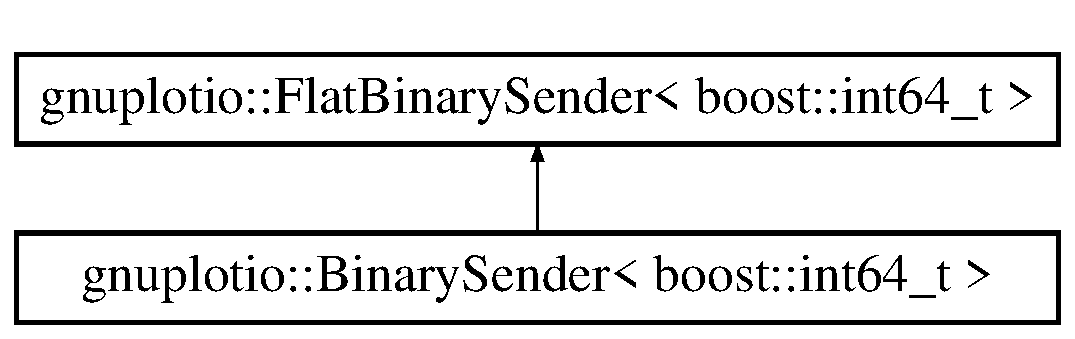
\includegraphics[height=2.000000cm]{structgnuplotio_1_1_binary_sender_3_01boost_1_1int64__t_01_4}
\end{center}
\end{figure}
\subsection*{Additional Inherited Members}


\subsection{Detailed Description}
\subsubsection*{template$<$$>$\\*
struct gnuplotio\+::\+Binary\+Sender$<$ boost\+::int64\+\_\+t $>$}



Definition at line 489 of file gnuplot-\/iostream.\+h.



The documentation for this struct was generated from the following file\+:\begin{DoxyCompactItemize}
\item 
include/\hyperlink{gnuplot-iostream_8h}{gnuplot-\/iostream.\+h}\end{DoxyCompactItemize}

\hypertarget{structgnuplotio_1_1_binary_sender_3_01boost_1_1int8__t_01_4}{}\section{gnuplotio\+:\+:Binary\+Sender$<$ boost\+:\+:int8\+\_\+t $>$ Struct Template Reference}
\label{structgnuplotio_1_1_binary_sender_3_01boost_1_1int8__t_01_4}\index{gnuplotio\+::\+Binary\+Sender$<$ boost\+::int8\+\_\+t $>$@{gnuplotio\+::\+Binary\+Sender$<$ boost\+::int8\+\_\+t $>$}}


{\ttfamily \#include $<$gnuplot-\/iostream.\+h$>$}

Inheritance diagram for gnuplotio\+:\+:Binary\+Sender$<$ boost\+:\+:int8\+\_\+t $>$\+:\begin{figure}[H]
\begin{center}
\leavevmode
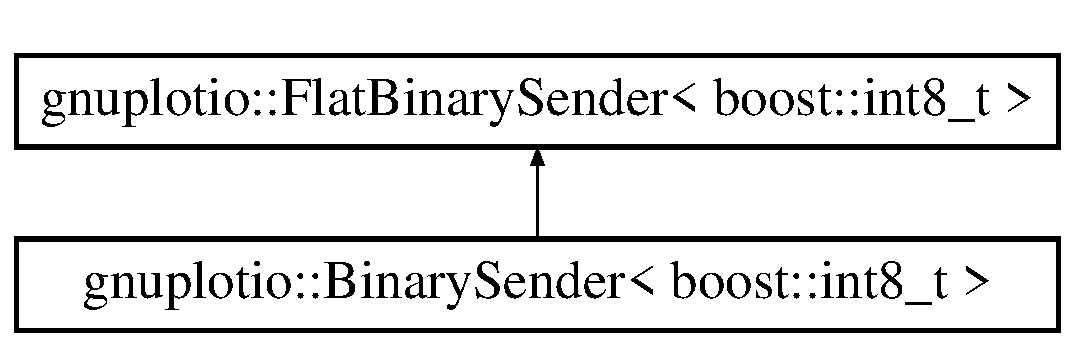
\includegraphics[height=2.000000cm]{structgnuplotio_1_1_binary_sender_3_01boost_1_1int8__t_01_4}
\end{center}
\end{figure}
\subsection*{Additional Inherited Members}


\subsection{Detailed Description}
\subsubsection*{template$<$$>$\\*
struct gnuplotio\+::\+Binary\+Sender$<$ boost\+::int8\+\_\+t $>$}



Definition at line 483 of file gnuplot-\/iostream.\+h.



The documentation for this struct was generated from the following file\+:\begin{DoxyCompactItemize}
\item 
include/\hyperlink{gnuplot-iostream_8h}{gnuplot-\/iostream.\+h}\end{DoxyCompactItemize}

\hypertarget{structgnuplotio_1_1_binary_sender_3_01boost_1_1uint16__t_01_4}{}\section{gnuplotio\+:\+:Binary\+Sender$<$ boost\+:\+:uint16\+\_\+t $>$ Struct Template Reference}
\label{structgnuplotio_1_1_binary_sender_3_01boost_1_1uint16__t_01_4}\index{gnuplotio\+::\+Binary\+Sender$<$ boost\+::uint16\+\_\+t $>$@{gnuplotio\+::\+Binary\+Sender$<$ boost\+::uint16\+\_\+t $>$}}


{\ttfamily \#include $<$gnuplot-\/iostream.\+h$>$}

Inheritance diagram for gnuplotio\+:\+:Binary\+Sender$<$ boost\+:\+:uint16\+\_\+t $>$\+:\begin{figure}[H]
\begin{center}
\leavevmode
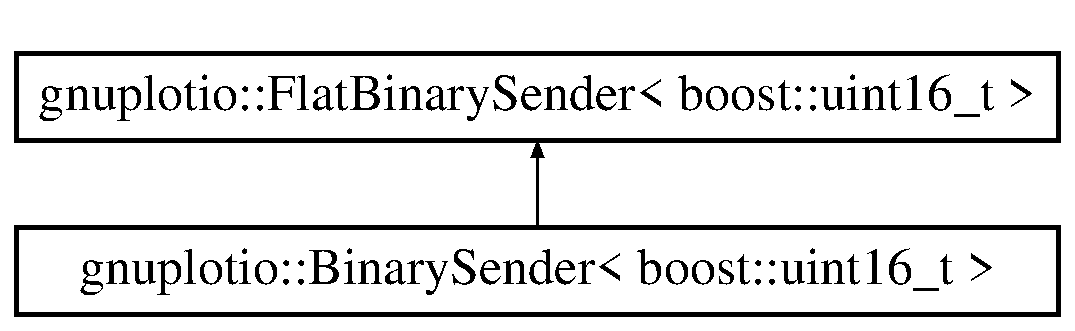
\includegraphics[height=2.000000cm]{structgnuplotio_1_1_binary_sender_3_01boost_1_1uint16__t_01_4}
\end{center}
\end{figure}
\subsection*{Additional Inherited Members}


\subsection{Detailed Description}
\subsubsection*{template$<$$>$\\*
struct gnuplotio\+::\+Binary\+Sender$<$ boost\+::uint16\+\_\+t $>$}



Definition at line 486 of file gnuplot-\/iostream.\+h.



The documentation for this struct was generated from the following file\+:\begin{DoxyCompactItemize}
\item 
include/\hyperlink{gnuplot-iostream_8h}{gnuplot-\/iostream.\+h}\end{DoxyCompactItemize}

\hypertarget{structgnuplotio_1_1_binary_sender_3_01boost_1_1uint32__t_01_4}{}\section{gnuplotio\+:\+:Binary\+Sender$<$ boost\+:\+:uint32\+\_\+t $>$ Struct Template Reference}
\label{structgnuplotio_1_1_binary_sender_3_01boost_1_1uint32__t_01_4}\index{gnuplotio\+::\+Binary\+Sender$<$ boost\+::uint32\+\_\+t $>$@{gnuplotio\+::\+Binary\+Sender$<$ boost\+::uint32\+\_\+t $>$}}


{\ttfamily \#include $<$gnuplot-\/iostream.\+h$>$}

Inheritance diagram for gnuplotio\+:\+:Binary\+Sender$<$ boost\+:\+:uint32\+\_\+t $>$\+:\begin{figure}[H]
\begin{center}
\leavevmode
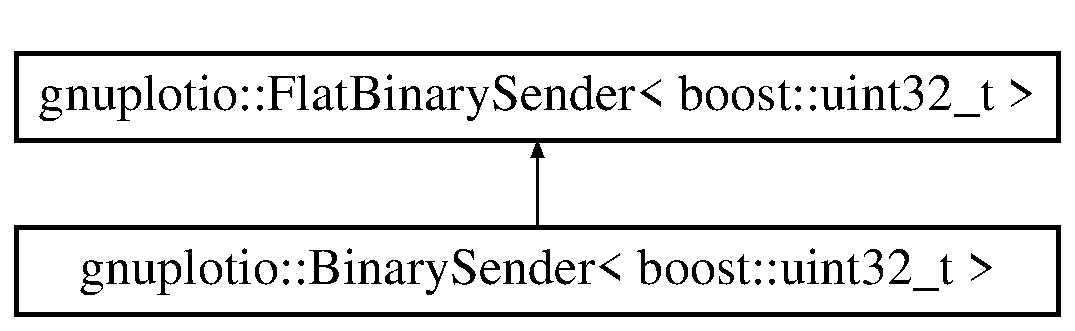
\includegraphics[height=2.000000cm]{structgnuplotio_1_1_binary_sender_3_01boost_1_1uint32__t_01_4}
\end{center}
\end{figure}
\subsection*{Additional Inherited Members}


\subsection{Detailed Description}
\subsubsection*{template$<$$>$\\*
struct gnuplotio\+::\+Binary\+Sender$<$ boost\+::uint32\+\_\+t $>$}



Definition at line 488 of file gnuplot-\/iostream.\+h.



The documentation for this struct was generated from the following file\+:\begin{DoxyCompactItemize}
\item 
include/\hyperlink{gnuplot-iostream_8h}{gnuplot-\/iostream.\+h}\end{DoxyCompactItemize}

\hypertarget{structgnuplotio_1_1_binary_sender_3_01boost_1_1uint64__t_01_4}{}\section{gnuplotio\+:\+:Binary\+Sender$<$ boost\+:\+:uint64\+\_\+t $>$ Struct Template Reference}
\label{structgnuplotio_1_1_binary_sender_3_01boost_1_1uint64__t_01_4}\index{gnuplotio\+::\+Binary\+Sender$<$ boost\+::uint64\+\_\+t $>$@{gnuplotio\+::\+Binary\+Sender$<$ boost\+::uint64\+\_\+t $>$}}


{\ttfamily \#include $<$gnuplot-\/iostream.\+h$>$}

Inheritance diagram for gnuplotio\+:\+:Binary\+Sender$<$ boost\+:\+:uint64\+\_\+t $>$\+:\begin{figure}[H]
\begin{center}
\leavevmode
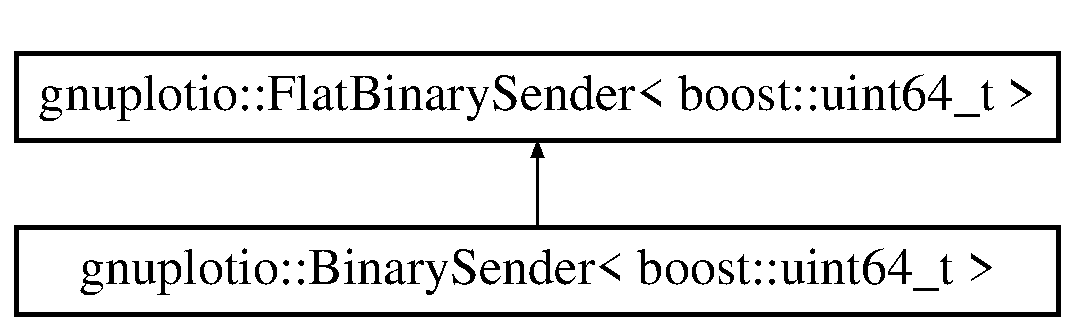
\includegraphics[height=2.000000cm]{structgnuplotio_1_1_binary_sender_3_01boost_1_1uint64__t_01_4}
\end{center}
\end{figure}
\subsection*{Additional Inherited Members}


\subsection{Detailed Description}
\subsubsection*{template$<$$>$\\*
struct gnuplotio\+::\+Binary\+Sender$<$ boost\+::uint64\+\_\+t $>$}



Definition at line 490 of file gnuplot-\/iostream.\+h.



The documentation for this struct was generated from the following file\+:\begin{DoxyCompactItemize}
\item 
include/\hyperlink{gnuplot-iostream_8h}{gnuplot-\/iostream.\+h}\end{DoxyCompactItemize}

\hypertarget{structgnuplotio_1_1_binary_sender_3_01boost_1_1uint8__t_01_4}{}\section{gnuplotio\+:\+:Binary\+Sender$<$ boost\+:\+:uint8\+\_\+t $>$ Struct Template Reference}
\label{structgnuplotio_1_1_binary_sender_3_01boost_1_1uint8__t_01_4}\index{gnuplotio\+::\+Binary\+Sender$<$ boost\+::uint8\+\_\+t $>$@{gnuplotio\+::\+Binary\+Sender$<$ boost\+::uint8\+\_\+t $>$}}


{\ttfamily \#include $<$gnuplot-\/iostream.\+h$>$}

Inheritance diagram for gnuplotio\+:\+:Binary\+Sender$<$ boost\+:\+:uint8\+\_\+t $>$\+:\begin{figure}[H]
\begin{center}
\leavevmode
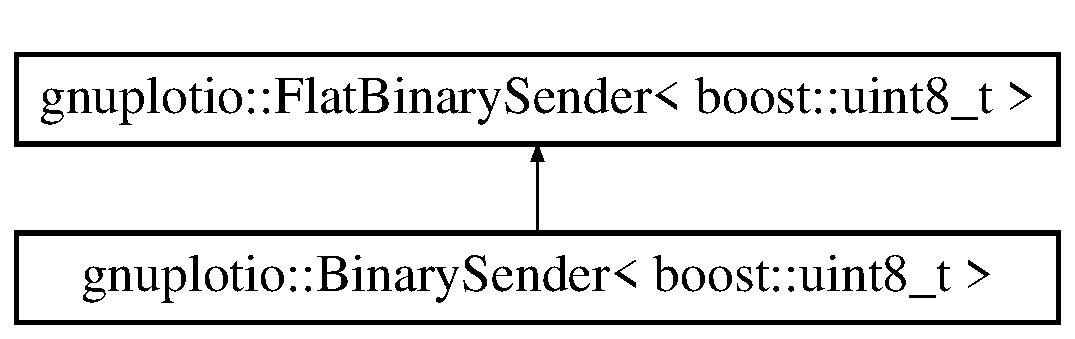
\includegraphics[height=2.000000cm]{structgnuplotio_1_1_binary_sender_3_01boost_1_1uint8__t_01_4}
\end{center}
\end{figure}
\subsection*{Additional Inherited Members}


\subsection{Detailed Description}
\subsubsection*{template$<$$>$\\*
struct gnuplotio\+::\+Binary\+Sender$<$ boost\+::uint8\+\_\+t $>$}



Definition at line 484 of file gnuplot-\/iostream.\+h.



The documentation for this struct was generated from the following file\+:\begin{DoxyCompactItemize}
\item 
include/\hyperlink{gnuplot-iostream_8h}{gnuplot-\/iostream.\+h}\end{DoxyCompactItemize}

\hypertarget{structgnuplotio_1_1_binary_sender_3_01double_01_4}{}\section{gnuplotio\+:\+:Binary\+Sender$<$ double $>$ Struct Template Reference}
\label{structgnuplotio_1_1_binary_sender_3_01double_01_4}\index{gnuplotio\+::\+Binary\+Sender$<$ double $>$@{gnuplotio\+::\+Binary\+Sender$<$ double $>$}}


{\ttfamily \#include $<$gnuplot-\/iostream.\+h$>$}

Inheritance diagram for gnuplotio\+:\+:Binary\+Sender$<$ double $>$\+:\begin{figure}[H]
\begin{center}
\leavevmode
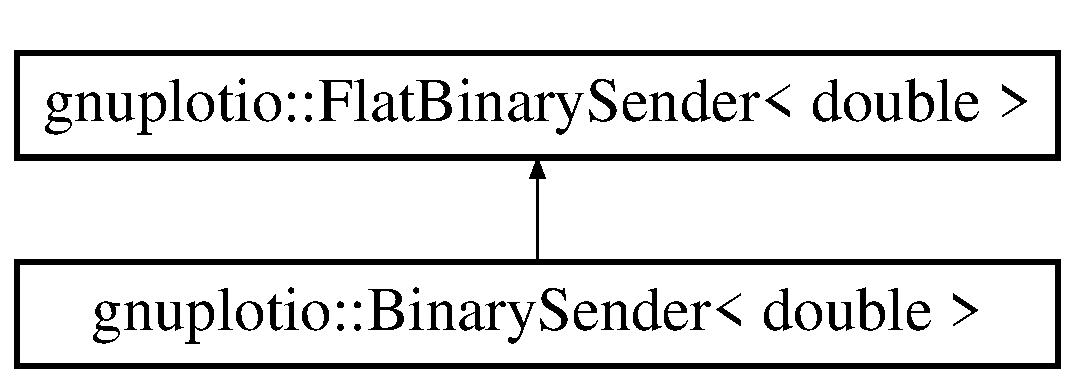
\includegraphics[height=2.000000cm]{structgnuplotio_1_1_binary_sender_3_01double_01_4}
\end{center}
\end{figure}
\subsection*{Additional Inherited Members}


\subsection{Detailed Description}
\subsubsection*{template$<$$>$\\*
struct gnuplotio\+::\+Binary\+Sender$<$ double $>$}



Definition at line 482 of file gnuplot-\/iostream.\+h.



The documentation for this struct was generated from the following file\+:\begin{DoxyCompactItemize}
\item 
include/\hyperlink{gnuplot-iostream_8h}{gnuplot-\/iostream.\+h}\end{DoxyCompactItemize}

\hypertarget{structgnuplotio_1_1_binary_sender_3_01float_01_4}{}\section{gnuplotio\+:\+:Binary\+Sender$<$ float $>$ Struct Template Reference}
\label{structgnuplotio_1_1_binary_sender_3_01float_01_4}\index{gnuplotio\+::\+Binary\+Sender$<$ float $>$@{gnuplotio\+::\+Binary\+Sender$<$ float $>$}}


{\ttfamily \#include $<$gnuplot-\/iostream.\+h$>$}

Inheritance diagram for gnuplotio\+:\+:Binary\+Sender$<$ float $>$\+:\begin{figure}[H]
\begin{center}
\leavevmode
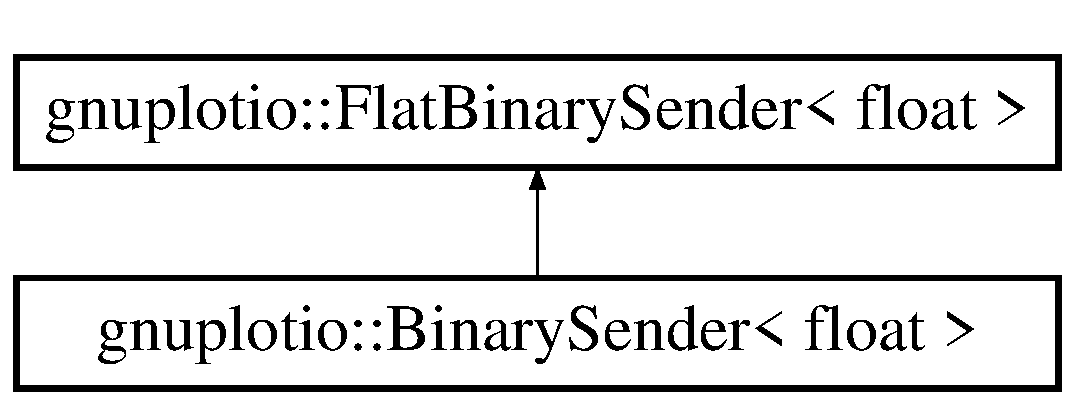
\includegraphics[height=2.000000cm]{structgnuplotio_1_1_binary_sender_3_01float_01_4}
\end{center}
\end{figure}
\subsection*{Additional Inherited Members}


\subsection{Detailed Description}
\subsubsection*{template$<$$>$\\*
struct gnuplotio\+::\+Binary\+Sender$<$ float $>$}



Definition at line 481 of file gnuplot-\/iostream.\+h.



The documentation for this struct was generated from the following file\+:\begin{DoxyCompactItemize}
\item 
include/\hyperlink{gnuplot-iostream_8h}{gnuplot-\/iostream.\+h}\end{DoxyCompactItemize}

\hypertarget{structgnuplotio_1_1_binary_sender_3_01std_1_1complex_3_01_t_01_4_01_4}{}\section{gnuplotio\+:\+:Binary\+Sender$<$ std\+:\+:complex$<$ T $>$ $>$ Struct Template Reference}
\label{structgnuplotio_1_1_binary_sender_3_01std_1_1complex_3_01_t_01_4_01_4}\index{gnuplotio\+::\+Binary\+Sender$<$ std\+::complex$<$ T $>$ $>$@{gnuplotio\+::\+Binary\+Sender$<$ std\+::complex$<$ T $>$ $>$}}


{\ttfamily \#include $<$gnuplot-\/iostream.\+h$>$}

\subsection*{Static Public Member Functions}
\begin{DoxyCompactItemize}
\item 
static void \hyperlink{structgnuplotio_1_1_binary_sender_3_01std_1_1complex_3_01_t_01_4_01_4_a759de700a1cd68000830a4b15a6fec49}{send} (std\+::ostream \&stream, const std\+::complex$<$ T $>$ \&v)
\end{DoxyCompactItemize}


\subsection{Detailed Description}
\subsubsection*{template$<$typename T$>$\\*
struct gnuplotio\+::\+Binary\+Sender$<$ std\+::complex$<$ T $>$ $>$}



Definition at line 565 of file gnuplot-\/iostream.\+h.



\subsection{Member Function Documentation}
\index{gnuplotio\+::\+Binary\+Sender$<$ std\+::complex$<$ T $>$ $>$@{gnuplotio\+::\+Binary\+Sender$<$ std\+::complex$<$ T $>$ $>$}!send@{send}}
\index{send@{send}!gnuplotio\+::\+Binary\+Sender$<$ std\+::complex$<$ T $>$ $>$@{gnuplotio\+::\+Binary\+Sender$<$ std\+::complex$<$ T $>$ $>$}}
\subsubsection[{\texorpdfstring{send(std\+::ostream \&stream, const std\+::complex$<$ T $>$ \&v)}{send(std::ostream &stream, const std::complex< T > &v)}}]{\setlength{\rightskip}{0pt plus 5cm}template$<$typename T $>$ static void {\bf gnuplotio\+::\+Binary\+Sender}$<$ std\+::complex$<$ T $>$ $>$\+::send (
\begin{DoxyParamCaption}
\item[{std\+::ostream \&}]{stream, }
\item[{const std\+::complex$<$ T $>$ \&}]{v}
\end{DoxyParamCaption}
)\hspace{0.3cm}{\ttfamily [inline]}, {\ttfamily [static]}}\hypertarget{structgnuplotio_1_1_binary_sender_3_01std_1_1complex_3_01_t_01_4_01_4_a759de700a1cd68000830a4b15a6fec49}{}\label{structgnuplotio_1_1_binary_sender_3_01std_1_1complex_3_01_t_01_4_01_4_a759de700a1cd68000830a4b15a6fec49}


Definition at line 566 of file gnuplot-\/iostream.\+h.



The documentation for this struct was generated from the following file\+:\begin{DoxyCompactItemize}
\item 
include/\hyperlink{gnuplot-iostream_8h}{gnuplot-\/iostream.\+h}\end{DoxyCompactItemize}

\hypertarget{structgnuplotio_1_1_binary_sender_3_01std_1_1pair_3_01_t_00_01_u_01_4_01_4}{}\section{gnuplotio\+:\+:Binary\+Sender$<$ std\+:\+:pair$<$ T, U $>$ $>$ Struct Template Reference}
\label{structgnuplotio_1_1_binary_sender_3_01std_1_1pair_3_01_t_00_01_u_01_4_01_4}\index{gnuplotio\+::\+Binary\+Sender$<$ std\+::pair$<$ T, U $>$ $>$@{gnuplotio\+::\+Binary\+Sender$<$ std\+::pair$<$ T, U $>$ $>$}}


{\ttfamily \#include $<$gnuplot-\/iostream.\+h$>$}

\subsection*{Static Public Member Functions}
\begin{DoxyCompactItemize}
\item 
static void \hyperlink{structgnuplotio_1_1_binary_sender_3_01std_1_1pair_3_01_t_00_01_u_01_4_01_4_a9d949c8e7b1dea493288b0a2dd95cbff}{send} (std\+::ostream \&stream, const std\+::pair$<$ T, U $>$ \&v)
\end{DoxyCompactItemize}


\subsection{Detailed Description}
\subsubsection*{template$<$typename T, typename U$>$\\*
struct gnuplotio\+::\+Binary\+Sender$<$ std\+::pair$<$ T, U $>$ $>$}



Definition at line 536 of file gnuplot-\/iostream.\+h.



\subsection{Member Function Documentation}
\index{gnuplotio\+::\+Binary\+Sender$<$ std\+::pair$<$ T, U $>$ $>$@{gnuplotio\+::\+Binary\+Sender$<$ std\+::pair$<$ T, U $>$ $>$}!send@{send}}
\index{send@{send}!gnuplotio\+::\+Binary\+Sender$<$ std\+::pair$<$ T, U $>$ $>$@{gnuplotio\+::\+Binary\+Sender$<$ std\+::pair$<$ T, U $>$ $>$}}
\subsubsection[{\texorpdfstring{send(std\+::ostream \&stream, const std\+::pair$<$ T, U $>$ \&v)}{send(std::ostream &stream, const std::pair< T, U > &v)}}]{\setlength{\rightskip}{0pt plus 5cm}template$<$typename T , typename U $>$ static void {\bf gnuplotio\+::\+Binary\+Sender}$<$ std\+::pair$<$ T, U $>$ $>$\+::send (
\begin{DoxyParamCaption}
\item[{std\+::ostream \&}]{stream, }
\item[{const std\+::pair$<$ T, U $>$ \&}]{v}
\end{DoxyParamCaption}
)\hspace{0.3cm}{\ttfamily [inline]}, {\ttfamily [static]}}\hypertarget{structgnuplotio_1_1_binary_sender_3_01std_1_1pair_3_01_t_00_01_u_01_4_01_4_a9d949c8e7b1dea493288b0a2dd95cbff}{}\label{structgnuplotio_1_1_binary_sender_3_01std_1_1pair_3_01_t_00_01_u_01_4_01_4_a9d949c8e7b1dea493288b0a2dd95cbff}


Definition at line 537 of file gnuplot-\/iostream.\+h.



The documentation for this struct was generated from the following file\+:\begin{DoxyCompactItemize}
\item 
include/\hyperlink{gnuplot-iostream_8h}{gnuplot-\/iostream.\+h}\end{DoxyCompactItemize}

\hypertarget{structgnuplotio_1_1_binary_sender_3_01_t_00_01typename_01boost_1_1enable__if_3_01boost_1_1mpl_1_916ff7a758aa0b8917fd3b30ff275f06}{}\section{gnuplotio\+:\+:Binary\+Sender$<$ T, typename boost\+:\+:enable\+\_\+if$<$ boost\+:\+:mpl\+:\+:and\+\_\+$<$ is\+\_\+boost\+\_\+tuple$<$ T $>$, boost\+:\+:mpl\+:\+:not\+\_\+$<$ is\+\_\+boost\+\_\+tuple\+\_\+nulltype$<$ typename T\+:\+:tail\+\_\+type $>$ $>$ $>$ $>$\+:\+:type $>$ Struct Template Reference}
\label{structgnuplotio_1_1_binary_sender_3_01_t_00_01typename_01boost_1_1enable__if_3_01boost_1_1mpl_1_916ff7a758aa0b8917fd3b30ff275f06}\index{gnuplotio\+::\+Binary\+Sender$<$ T, typename boost\+::enable\+\_\+if$<$ boost\+::mpl\+::and\+\_\+$<$ is\+\_\+boost\+\_\+tuple$<$ T $>$, boost\+::mpl\+::not\+\_\+$<$ is\+\_\+boost\+\_\+tuple\+\_\+nulltype$<$ typename T\+::tail\+\_\+type $>$ $>$ $>$ $>$\+::type $>$@{gnuplotio\+::\+Binary\+Sender$<$ T, typename boost\+::enable\+\_\+if$<$ boost\+::mpl\+::and\+\_\+$<$ is\+\_\+boost\+\_\+tuple$<$ T $>$, boost\+::mpl\+::not\+\_\+$<$ is\+\_\+boost\+\_\+tuple\+\_\+nulltype$<$ typename T\+::tail\+\_\+type $>$ $>$ $>$ $>$\+::type $>$}}


{\ttfamily \#include $<$gnuplot-\/iostream.\+h$>$}

\subsection*{Static Public Member Functions}
\begin{DoxyCompactItemize}
\item 
static void \hyperlink{structgnuplotio_1_1_binary_sender_3_01_t_00_01typename_01boost_1_1enable__if_3_01boost_1_1mpl_1_916ff7a758aa0b8917fd3b30ff275f06_a90bdbe9d299646a871882da19fdb30a9}{send} (std\+::ostream \&stream, const T \&v)
\end{DoxyCompactItemize}


\subsection{Detailed Description}
\subsubsection*{template$<$typename T$>$\\*
struct gnuplotio\+::\+Binary\+Sender$<$ T, typename boost\+::enable\+\_\+if$<$ boost\+::mpl\+::and\+\_\+$<$ is\+\_\+boost\+\_\+tuple$<$ T $>$, boost\+::mpl\+::not\+\_\+$<$ is\+\_\+boost\+\_\+tuple\+\_\+nulltype$<$ typename T\+::tail\+\_\+type $>$ $>$ $>$ $>$\+::type $>$}



Definition at line 637 of file gnuplot-\/iostream.\+h.



\subsection{Member Function Documentation}
\index{gnuplotio\+::\+Binary\+Sender$<$ T, typename boost\+::enable\+\_\+if$<$ boost\+::mpl\+::and\+\_\+$<$ is\+\_\+boost\+\_\+tuple$<$ T $>$, boost\+::mpl\+::not\+\_\+$<$ is\+\_\+boost\+\_\+tuple\+\_\+nulltype$<$ typename T\+::tail\+\_\+type $>$ $>$ $>$ $>$\+::type $>$@{gnuplotio\+::\+Binary\+Sender$<$ T, typename boost\+::enable\+\_\+if$<$ boost\+::mpl\+::and\+\_\+$<$ is\+\_\+boost\+\_\+tuple$<$ T $>$, boost\+::mpl\+::not\+\_\+$<$ is\+\_\+boost\+\_\+tuple\+\_\+nulltype$<$ typename T\+::tail\+\_\+type $>$ $>$ $>$ $>$\+::type $>$}!send@{send}}
\index{send@{send}!gnuplotio\+::\+Binary\+Sender$<$ T, typename boost\+::enable\+\_\+if$<$ boost\+::mpl\+::and\+\_\+$<$ is\+\_\+boost\+\_\+tuple$<$ T $>$, boost\+::mpl\+::not\+\_\+$<$ is\+\_\+boost\+\_\+tuple\+\_\+nulltype$<$ typename T\+::tail\+\_\+type $>$ $>$ $>$ $>$\+::type $>$@{gnuplotio\+::\+Binary\+Sender$<$ T, typename boost\+::enable\+\_\+if$<$ boost\+::mpl\+::and\+\_\+$<$ is\+\_\+boost\+\_\+tuple$<$ T $>$, boost\+::mpl\+::not\+\_\+$<$ is\+\_\+boost\+\_\+tuple\+\_\+nulltype$<$ typename T\+::tail\+\_\+type $>$ $>$ $>$ $>$\+::type $>$}}
\subsubsection[{\texorpdfstring{send(std\+::ostream \&stream, const T \&v)}{send(std::ostream &stream, const T &v)}}]{\setlength{\rightskip}{0pt plus 5cm}template$<$typename T $>$ static void {\bf gnuplotio\+::\+Binary\+Sender}$<$ T, typename boost\+::enable\+\_\+if$<$ boost\+::mpl\+::and\+\_\+$<$ {\bf is\+\_\+boost\+\_\+tuple}$<$ T $>$, boost\+::mpl\+::not\+\_\+$<$ {\bf is\+\_\+boost\+\_\+tuple\+\_\+nulltype}$<$ typename T\+::tail\+\_\+type $>$ $>$ $>$ $>$\+::type $>$\+::send (
\begin{DoxyParamCaption}
\item[{std\+::ostream \&}]{stream, }
\item[{const T \&}]{v}
\end{DoxyParamCaption}
)\hspace{0.3cm}{\ttfamily [inline]}, {\ttfamily [static]}}\hypertarget{structgnuplotio_1_1_binary_sender_3_01_t_00_01typename_01boost_1_1enable__if_3_01boost_1_1mpl_1_916ff7a758aa0b8917fd3b30ff275f06_a90bdbe9d299646a871882da19fdb30a9}{}\label{structgnuplotio_1_1_binary_sender_3_01_t_00_01typename_01boost_1_1enable__if_3_01boost_1_1mpl_1_916ff7a758aa0b8917fd3b30ff275f06_a90bdbe9d299646a871882da19fdb30a9}


Definition at line 645 of file gnuplot-\/iostream.\+h.



The documentation for this struct was generated from the following file\+:\begin{DoxyCompactItemize}
\item 
include/\hyperlink{gnuplot-iostream_8h}{gnuplot-\/iostream.\+h}\end{DoxyCompactItemize}

\hypertarget{structgnuplotio_1_1_binary_sender_3_01_t_00_01typename_01boost_1_1enable__if_3_01boost_1_1mpl_1_29e1098ca8b7afc20f2ca0bc2e79506a}{}\section{gnuplotio\+:\+:Binary\+Sender$<$ T, typename boost\+:\+:enable\+\_\+if$<$ boost\+:\+:mpl\+:\+:and\+\_\+$<$ is\+\_\+boost\+\_\+tuple$<$ T $>$, is\+\_\+boost\+\_\+tuple\+\_\+nulltype$<$ typename T\+:\+:tail\+\_\+type $>$ $>$ $>$\+:\+:type $>$ Struct Template Reference}
\label{structgnuplotio_1_1_binary_sender_3_01_t_00_01typename_01boost_1_1enable__if_3_01boost_1_1mpl_1_29e1098ca8b7afc20f2ca0bc2e79506a}\index{gnuplotio\+::\+Binary\+Sender$<$ T, typename boost\+::enable\+\_\+if$<$ boost\+::mpl\+::and\+\_\+$<$ is\+\_\+boost\+\_\+tuple$<$ T $>$, is\+\_\+boost\+\_\+tuple\+\_\+nulltype$<$ typename T\+::tail\+\_\+type $>$ $>$ $>$\+::type $>$@{gnuplotio\+::\+Binary\+Sender$<$ T, typename boost\+::enable\+\_\+if$<$ boost\+::mpl\+::and\+\_\+$<$ is\+\_\+boost\+\_\+tuple$<$ T $>$, is\+\_\+boost\+\_\+tuple\+\_\+nulltype$<$ typename T\+::tail\+\_\+type $>$ $>$ $>$\+::type $>$}}


{\ttfamily \#include $<$gnuplot-\/iostream.\+h$>$}

\subsection*{Static Public Member Functions}
\begin{DoxyCompactItemize}
\item 
static void \hyperlink{structgnuplotio_1_1_binary_sender_3_01_t_00_01typename_01boost_1_1enable__if_3_01boost_1_1mpl_1_29e1098ca8b7afc20f2ca0bc2e79506a_a50e54b7f2aba37f1f9e63fa81941b6d6}{send} (std\+::ostream \&stream, const T \&v)
\end{DoxyCompactItemize}


\subsection{Detailed Description}
\subsubsection*{template$<$typename T$>$\\*
struct gnuplotio\+::\+Binary\+Sender$<$ T, typename boost\+::enable\+\_\+if$<$ boost\+::mpl\+::and\+\_\+$<$ is\+\_\+boost\+\_\+tuple$<$ T $>$, is\+\_\+boost\+\_\+tuple\+\_\+nulltype$<$ typename T\+::tail\+\_\+type $>$ $>$ $>$\+::type $>$}



Definition at line 652 of file gnuplot-\/iostream.\+h.



\subsection{Member Function Documentation}
\index{gnuplotio\+::\+Binary\+Sender$<$ T, typename boost\+::enable\+\_\+if$<$ boost\+::mpl\+::and\+\_\+$<$ is\+\_\+boost\+\_\+tuple$<$ T $>$, is\+\_\+boost\+\_\+tuple\+\_\+nulltype$<$ typename T\+::tail\+\_\+type $>$ $>$ $>$\+::type $>$@{gnuplotio\+::\+Binary\+Sender$<$ T, typename boost\+::enable\+\_\+if$<$ boost\+::mpl\+::and\+\_\+$<$ is\+\_\+boost\+\_\+tuple$<$ T $>$, is\+\_\+boost\+\_\+tuple\+\_\+nulltype$<$ typename T\+::tail\+\_\+type $>$ $>$ $>$\+::type $>$}!send@{send}}
\index{send@{send}!gnuplotio\+::\+Binary\+Sender$<$ T, typename boost\+::enable\+\_\+if$<$ boost\+::mpl\+::and\+\_\+$<$ is\+\_\+boost\+\_\+tuple$<$ T $>$, is\+\_\+boost\+\_\+tuple\+\_\+nulltype$<$ typename T\+::tail\+\_\+type $>$ $>$ $>$\+::type $>$@{gnuplotio\+::\+Binary\+Sender$<$ T, typename boost\+::enable\+\_\+if$<$ boost\+::mpl\+::and\+\_\+$<$ is\+\_\+boost\+\_\+tuple$<$ T $>$, is\+\_\+boost\+\_\+tuple\+\_\+nulltype$<$ typename T\+::tail\+\_\+type $>$ $>$ $>$\+::type $>$}}
\subsubsection[{\texorpdfstring{send(std\+::ostream \&stream, const T \&v)}{send(std::ostream &stream, const T &v)}}]{\setlength{\rightskip}{0pt plus 5cm}template$<$typename T $>$ static void {\bf gnuplotio\+::\+Binary\+Sender}$<$ T, typename boost\+::enable\+\_\+if$<$ boost\+::mpl\+::and\+\_\+$<$ {\bf is\+\_\+boost\+\_\+tuple}$<$ T $>$, {\bf is\+\_\+boost\+\_\+tuple\+\_\+nulltype}$<$ typename T\+::tail\+\_\+type $>$ $>$ $>$\+::type $>$\+::send (
\begin{DoxyParamCaption}
\item[{std\+::ostream \&}]{stream, }
\item[{const T \&}]{v}
\end{DoxyParamCaption}
)\hspace{0.3cm}{\ttfamily [inline]}, {\ttfamily [static]}}\hypertarget{structgnuplotio_1_1_binary_sender_3_01_t_00_01typename_01boost_1_1enable__if_3_01boost_1_1mpl_1_29e1098ca8b7afc20f2ca0bc2e79506a_a50e54b7f2aba37f1f9e63fa81941b6d6}{}\label{structgnuplotio_1_1_binary_sender_3_01_t_00_01typename_01boost_1_1enable__if_3_01boost_1_1mpl_1_29e1098ca8b7afc20f2ca0bc2e79506a_a50e54b7f2aba37f1f9e63fa81941b6d6}


Definition at line 660 of file gnuplot-\/iostream.\+h.



The documentation for this struct was generated from the following file\+:\begin{DoxyCompactItemize}
\item 
include/\hyperlink{gnuplot-iostream_8h}{gnuplot-\/iostream.\+h}\end{DoxyCompactItemize}

\hypertarget{structgnuplotio_1_1_binfmt_sender}{}\section{gnuplotio\+:\+:Binfmt\+Sender$<$ T, Enable $>$ Struct Template Reference}
\label{structgnuplotio_1_1_binfmt_sender}\index{gnuplotio\+::\+Binfmt\+Sender$<$ T, Enable $>$@{gnuplotio\+::\+Binfmt\+Sender$<$ T, Enable $>$}}


{\ttfamily \#include $<$gnuplot-\/iostream.\+h$>$}

\subsection*{Public Member Functions}
\begin{DoxyCompactItemize}
\item 
\hyperlink{structgnuplotio_1_1_binfmt_sender_ab0b554a2e81309917b2fa6f480e2a8e2}{G\+N\+U\+P\+L\+O\+T\+\_\+\+S\+T\+A\+T\+I\+C\+\_\+\+A\+S\+S\+E\+R\+T\+\_\+\+M\+SG} ((sizeof(T)==0),\char`\"{}Binfmt\+Sender class not specialized for this type\char`\"{})
\end{DoxyCompactItemize}
\subsection*{Static Public Member Functions}
\begin{DoxyCompactItemize}
\item 
static void \hyperlink{structgnuplotio_1_1_binfmt_sender_a762010e3172c02e981252f93185b29c8}{send} (std\+::ostream \&)
\end{DoxyCompactItemize}


\subsection{Detailed Description}
\subsubsection*{template$<$typename T, typename Enable = void$>$\\*
struct gnuplotio\+::\+Binfmt\+Sender$<$ T, Enable $>$}



Definition at line 459 of file gnuplot-\/iostream.\+h.



\subsection{Member Function Documentation}
\index{gnuplotio\+::\+Binfmt\+Sender@{gnuplotio\+::\+Binfmt\+Sender}!G\+N\+U\+P\+L\+O\+T\+\_\+\+S\+T\+A\+T\+I\+C\+\_\+\+A\+S\+S\+E\+R\+T\+\_\+\+M\+SG@{G\+N\+U\+P\+L\+O\+T\+\_\+\+S\+T\+A\+T\+I\+C\+\_\+\+A\+S\+S\+E\+R\+T\+\_\+\+M\+SG}}
\index{G\+N\+U\+P\+L\+O\+T\+\_\+\+S\+T\+A\+T\+I\+C\+\_\+\+A\+S\+S\+E\+R\+T\+\_\+\+M\+SG@{G\+N\+U\+P\+L\+O\+T\+\_\+\+S\+T\+A\+T\+I\+C\+\_\+\+A\+S\+S\+E\+R\+T\+\_\+\+M\+SG}!gnuplotio\+::\+Binfmt\+Sender@{gnuplotio\+::\+Binfmt\+Sender}}
\subsubsection[{\texorpdfstring{G\+N\+U\+P\+L\+O\+T\+\_\+\+S\+T\+A\+T\+I\+C\+\_\+\+A\+S\+S\+E\+R\+T\+\_\+\+M\+S\+G((sizeof(\+T)==0),""Binfmt\+Sender class not specialized for this type"")}{GNUPLOT_STATIC_ASSERT_MSG((sizeof(T)==0),"BinfmtSender class not specialized for this type")}}]{\setlength{\rightskip}{0pt plus 5cm}template$<$typename T, typename Enable = void$>$ {\bf gnuplotio\+::\+Binfmt\+Sender}$<$ T, Enable $>$\+::G\+N\+U\+P\+L\+O\+T\+\_\+\+S\+T\+A\+T\+I\+C\+\_\+\+A\+S\+S\+E\+R\+T\+\_\+\+M\+SG (
\begin{DoxyParamCaption}
\item[{(sizeof(T)==0)}]{, }
\item[{\char`\"{}Binfmt\+Sender$<$ T, Enable $>$ class not specialized for this type\char`\"{}}]{}
\end{DoxyParamCaption}
)}\hypertarget{structgnuplotio_1_1_binfmt_sender_ab0b554a2e81309917b2fa6f480e2a8e2}{}\label{structgnuplotio_1_1_binfmt_sender_ab0b554a2e81309917b2fa6f480e2a8e2}
\index{gnuplotio\+::\+Binfmt\+Sender@{gnuplotio\+::\+Binfmt\+Sender}!send@{send}}
\index{send@{send}!gnuplotio\+::\+Binfmt\+Sender@{gnuplotio\+::\+Binfmt\+Sender}}
\subsubsection[{\texorpdfstring{send(std\+::ostream \&)}{send(std::ostream &)}}]{\setlength{\rightskip}{0pt plus 5cm}template$<$typename T, typename Enable = void$>$ static void {\bf gnuplotio\+::\+Binfmt\+Sender}$<$ T, Enable $>$\+::send (
\begin{DoxyParamCaption}
\item[{std\+::ostream \&}]{}
\end{DoxyParamCaption}
)\hspace{0.3cm}{\ttfamily [static]}}\hypertarget{structgnuplotio_1_1_binfmt_sender_a762010e3172c02e981252f93185b29c8}{}\label{structgnuplotio_1_1_binfmt_sender_a762010e3172c02e981252f93185b29c8}


The documentation for this struct was generated from the following file\+:\begin{DoxyCompactItemize}
\item 
include/\hyperlink{gnuplot-iostream_8h}{gnuplot-\/iostream.\+h}\end{DoxyCompactItemize}

\hypertarget{structgnuplotio_1_1_binfmt_sender_3_01boost_1_1int16__t_01_4}{}\section{gnuplotio\+:\+:Binfmt\+Sender$<$ boost\+:\+:int16\+\_\+t $>$ Struct Template Reference}
\label{structgnuplotio_1_1_binfmt_sender_3_01boost_1_1int16__t_01_4}\index{gnuplotio\+::\+Binfmt\+Sender$<$ boost\+::int16\+\_\+t $>$@{gnuplotio\+::\+Binfmt\+Sender$<$ boost\+::int16\+\_\+t $>$}}


{\ttfamily \#include $<$gnuplot-\/iostream.\+h$>$}

\subsection*{Static Public Member Functions}
\begin{DoxyCompactItemize}
\item 
static void \hyperlink{structgnuplotio_1_1_binfmt_sender_3_01boost_1_1int16__t_01_4_a6d3c1b829c9196fa9d1f53bd78a90e34}{send} (std\+::ostream \&stream)
\end{DoxyCompactItemize}


\subsection{Detailed Description}
\subsubsection*{template$<$$>$\\*
struct gnuplotio\+::\+Binfmt\+Sender$<$ boost\+::int16\+\_\+t $>$}



Definition at line 472 of file gnuplot-\/iostream.\+h.



\subsection{Member Function Documentation}
\index{gnuplotio\+::\+Binfmt\+Sender$<$ boost\+::int16\+\_\+t $>$@{gnuplotio\+::\+Binfmt\+Sender$<$ boost\+::int16\+\_\+t $>$}!send@{send}}
\index{send@{send}!gnuplotio\+::\+Binfmt\+Sender$<$ boost\+::int16\+\_\+t $>$@{gnuplotio\+::\+Binfmt\+Sender$<$ boost\+::int16\+\_\+t $>$}}
\subsubsection[{\texorpdfstring{send(std\+::ostream \&stream)}{send(std::ostream &stream)}}]{\setlength{\rightskip}{0pt plus 5cm}static void {\bf gnuplotio\+::\+Binfmt\+Sender}$<$ boost\+::int16\+\_\+t $>$\+::send (
\begin{DoxyParamCaption}
\item[{std\+::ostream \&}]{stream}
\end{DoxyParamCaption}
)\hspace{0.3cm}{\ttfamily [inline]}, {\ttfamily [static]}}\hypertarget{structgnuplotio_1_1_binfmt_sender_3_01boost_1_1int16__t_01_4_a6d3c1b829c9196fa9d1f53bd78a90e34}{}\label{structgnuplotio_1_1_binfmt_sender_3_01boost_1_1int16__t_01_4_a6d3c1b829c9196fa9d1f53bd78a90e34}


Definition at line 472 of file gnuplot-\/iostream.\+h.



The documentation for this struct was generated from the following file\+:\begin{DoxyCompactItemize}
\item 
include/\hyperlink{gnuplot-iostream_8h}{gnuplot-\/iostream.\+h}\end{DoxyCompactItemize}

\hypertarget{structgnuplotio_1_1_binfmt_sender_3_01boost_1_1int32__t_01_4}{}\section{gnuplotio\+:\+:Binfmt\+Sender$<$ boost\+:\+:int32\+\_\+t $>$ Struct Template Reference}
\label{structgnuplotio_1_1_binfmt_sender_3_01boost_1_1int32__t_01_4}\index{gnuplotio\+::\+Binfmt\+Sender$<$ boost\+::int32\+\_\+t $>$@{gnuplotio\+::\+Binfmt\+Sender$<$ boost\+::int32\+\_\+t $>$}}


{\ttfamily \#include $<$gnuplot-\/iostream.\+h$>$}

\subsection*{Static Public Member Functions}
\begin{DoxyCompactItemize}
\item 
static void \hyperlink{structgnuplotio_1_1_binfmt_sender_3_01boost_1_1int32__t_01_4_a44f75b80ef3f5def62eaa2093810fd35}{send} (std\+::ostream \&stream)
\end{DoxyCompactItemize}


\subsection{Detailed Description}
\subsubsection*{template$<$$>$\\*
struct gnuplotio\+::\+Binfmt\+Sender$<$ boost\+::int32\+\_\+t $>$}



Definition at line 474 of file gnuplot-\/iostream.\+h.



\subsection{Member Function Documentation}
\index{gnuplotio\+::\+Binfmt\+Sender$<$ boost\+::int32\+\_\+t $>$@{gnuplotio\+::\+Binfmt\+Sender$<$ boost\+::int32\+\_\+t $>$}!send@{send}}
\index{send@{send}!gnuplotio\+::\+Binfmt\+Sender$<$ boost\+::int32\+\_\+t $>$@{gnuplotio\+::\+Binfmt\+Sender$<$ boost\+::int32\+\_\+t $>$}}
\subsubsection[{\texorpdfstring{send(std\+::ostream \&stream)}{send(std::ostream &stream)}}]{\setlength{\rightskip}{0pt plus 5cm}static void {\bf gnuplotio\+::\+Binfmt\+Sender}$<$ boost\+::int32\+\_\+t $>$\+::send (
\begin{DoxyParamCaption}
\item[{std\+::ostream \&}]{stream}
\end{DoxyParamCaption}
)\hspace{0.3cm}{\ttfamily [inline]}, {\ttfamily [static]}}\hypertarget{structgnuplotio_1_1_binfmt_sender_3_01boost_1_1int32__t_01_4_a44f75b80ef3f5def62eaa2093810fd35}{}\label{structgnuplotio_1_1_binfmt_sender_3_01boost_1_1int32__t_01_4_a44f75b80ef3f5def62eaa2093810fd35}


Definition at line 474 of file gnuplot-\/iostream.\+h.



The documentation for this struct was generated from the following file\+:\begin{DoxyCompactItemize}
\item 
include/\hyperlink{gnuplot-iostream_8h}{gnuplot-\/iostream.\+h}\end{DoxyCompactItemize}

\hypertarget{structgnuplotio_1_1_binfmt_sender_3_01boost_1_1int64__t_01_4}{}\section{gnuplotio\+:\+:Binfmt\+Sender$<$ boost\+:\+:int64\+\_\+t $>$ Struct Template Reference}
\label{structgnuplotio_1_1_binfmt_sender_3_01boost_1_1int64__t_01_4}\index{gnuplotio\+::\+Binfmt\+Sender$<$ boost\+::int64\+\_\+t $>$@{gnuplotio\+::\+Binfmt\+Sender$<$ boost\+::int64\+\_\+t $>$}}


{\ttfamily \#include $<$gnuplot-\/iostream.\+h$>$}

\subsection*{Static Public Member Functions}
\begin{DoxyCompactItemize}
\item 
static void \hyperlink{structgnuplotio_1_1_binfmt_sender_3_01boost_1_1int64__t_01_4_a57423f02a4526e15d7d821606b1c8c81}{send} (std\+::ostream \&stream)
\end{DoxyCompactItemize}


\subsection{Detailed Description}
\subsubsection*{template$<$$>$\\*
struct gnuplotio\+::\+Binfmt\+Sender$<$ boost\+::int64\+\_\+t $>$}



Definition at line 476 of file gnuplot-\/iostream.\+h.



\subsection{Member Function Documentation}
\index{gnuplotio\+::\+Binfmt\+Sender$<$ boost\+::int64\+\_\+t $>$@{gnuplotio\+::\+Binfmt\+Sender$<$ boost\+::int64\+\_\+t $>$}!send@{send}}
\index{send@{send}!gnuplotio\+::\+Binfmt\+Sender$<$ boost\+::int64\+\_\+t $>$@{gnuplotio\+::\+Binfmt\+Sender$<$ boost\+::int64\+\_\+t $>$}}
\subsubsection[{\texorpdfstring{send(std\+::ostream \&stream)}{send(std::ostream &stream)}}]{\setlength{\rightskip}{0pt plus 5cm}static void {\bf gnuplotio\+::\+Binfmt\+Sender}$<$ boost\+::int64\+\_\+t $>$\+::send (
\begin{DoxyParamCaption}
\item[{std\+::ostream \&}]{stream}
\end{DoxyParamCaption}
)\hspace{0.3cm}{\ttfamily [inline]}, {\ttfamily [static]}}\hypertarget{structgnuplotio_1_1_binfmt_sender_3_01boost_1_1int64__t_01_4_a57423f02a4526e15d7d821606b1c8c81}{}\label{structgnuplotio_1_1_binfmt_sender_3_01boost_1_1int64__t_01_4_a57423f02a4526e15d7d821606b1c8c81}


Definition at line 476 of file gnuplot-\/iostream.\+h.



The documentation for this struct was generated from the following file\+:\begin{DoxyCompactItemize}
\item 
include/\hyperlink{gnuplot-iostream_8h}{gnuplot-\/iostream.\+h}\end{DoxyCompactItemize}

\hypertarget{structgnuplotio_1_1_binfmt_sender_3_01boost_1_1int8__t_01_4}{}\section{gnuplotio\+:\+:Binfmt\+Sender$<$ boost\+:\+:int8\+\_\+t $>$ Struct Template Reference}
\label{structgnuplotio_1_1_binfmt_sender_3_01boost_1_1int8__t_01_4}\index{gnuplotio\+::\+Binfmt\+Sender$<$ boost\+::int8\+\_\+t $>$@{gnuplotio\+::\+Binfmt\+Sender$<$ boost\+::int8\+\_\+t $>$}}


{\ttfamily \#include $<$gnuplot-\/iostream.\+h$>$}

\subsection*{Static Public Member Functions}
\begin{DoxyCompactItemize}
\item 
static void \hyperlink{structgnuplotio_1_1_binfmt_sender_3_01boost_1_1int8__t_01_4_a6f61d43b0da25f044bfad0d45fe888b4}{send} (std\+::ostream \&stream)
\end{DoxyCompactItemize}


\subsection{Detailed Description}
\subsubsection*{template$<$$>$\\*
struct gnuplotio\+::\+Binfmt\+Sender$<$ boost\+::int8\+\_\+t $>$}



Definition at line 470 of file gnuplot-\/iostream.\+h.



\subsection{Member Function Documentation}
\index{gnuplotio\+::\+Binfmt\+Sender$<$ boost\+::int8\+\_\+t $>$@{gnuplotio\+::\+Binfmt\+Sender$<$ boost\+::int8\+\_\+t $>$}!send@{send}}
\index{send@{send}!gnuplotio\+::\+Binfmt\+Sender$<$ boost\+::int8\+\_\+t $>$@{gnuplotio\+::\+Binfmt\+Sender$<$ boost\+::int8\+\_\+t $>$}}
\subsubsection[{\texorpdfstring{send(std\+::ostream \&stream)}{send(std::ostream &stream)}}]{\setlength{\rightskip}{0pt plus 5cm}static void {\bf gnuplotio\+::\+Binfmt\+Sender}$<$ boost\+::int8\+\_\+t $>$\+::send (
\begin{DoxyParamCaption}
\item[{std\+::ostream \&}]{stream}
\end{DoxyParamCaption}
)\hspace{0.3cm}{\ttfamily [inline]}, {\ttfamily [static]}}\hypertarget{structgnuplotio_1_1_binfmt_sender_3_01boost_1_1int8__t_01_4_a6f61d43b0da25f044bfad0d45fe888b4}{}\label{structgnuplotio_1_1_binfmt_sender_3_01boost_1_1int8__t_01_4_a6f61d43b0da25f044bfad0d45fe888b4}


Definition at line 470 of file gnuplot-\/iostream.\+h.



The documentation for this struct was generated from the following file\+:\begin{DoxyCompactItemize}
\item 
include/\hyperlink{gnuplot-iostream_8h}{gnuplot-\/iostream.\+h}\end{DoxyCompactItemize}

\hypertarget{structgnuplotio_1_1_binfmt_sender_3_01boost_1_1uint16__t_01_4}{}\section{gnuplotio\+:\+:Binfmt\+Sender$<$ boost\+:\+:uint16\+\_\+t $>$ Struct Template Reference}
\label{structgnuplotio_1_1_binfmt_sender_3_01boost_1_1uint16__t_01_4}\index{gnuplotio\+::\+Binfmt\+Sender$<$ boost\+::uint16\+\_\+t $>$@{gnuplotio\+::\+Binfmt\+Sender$<$ boost\+::uint16\+\_\+t $>$}}


{\ttfamily \#include $<$gnuplot-\/iostream.\+h$>$}

\subsection*{Static Public Member Functions}
\begin{DoxyCompactItemize}
\item 
static void \hyperlink{structgnuplotio_1_1_binfmt_sender_3_01boost_1_1uint16__t_01_4_a7bb7f0a62a21496b9e85ce35f0170717}{send} (std\+::ostream \&stream)
\end{DoxyCompactItemize}


\subsection{Detailed Description}
\subsubsection*{template$<$$>$\\*
struct gnuplotio\+::\+Binfmt\+Sender$<$ boost\+::uint16\+\_\+t $>$}



Definition at line 473 of file gnuplot-\/iostream.\+h.



\subsection{Member Function Documentation}
\index{gnuplotio\+::\+Binfmt\+Sender$<$ boost\+::uint16\+\_\+t $>$@{gnuplotio\+::\+Binfmt\+Sender$<$ boost\+::uint16\+\_\+t $>$}!send@{send}}
\index{send@{send}!gnuplotio\+::\+Binfmt\+Sender$<$ boost\+::uint16\+\_\+t $>$@{gnuplotio\+::\+Binfmt\+Sender$<$ boost\+::uint16\+\_\+t $>$}}
\subsubsection[{\texorpdfstring{send(std\+::ostream \&stream)}{send(std::ostream &stream)}}]{\setlength{\rightskip}{0pt plus 5cm}static void {\bf gnuplotio\+::\+Binfmt\+Sender}$<$ boost\+::uint16\+\_\+t $>$\+::send (
\begin{DoxyParamCaption}
\item[{std\+::ostream \&}]{stream}
\end{DoxyParamCaption}
)\hspace{0.3cm}{\ttfamily [inline]}, {\ttfamily [static]}}\hypertarget{structgnuplotio_1_1_binfmt_sender_3_01boost_1_1uint16__t_01_4_a7bb7f0a62a21496b9e85ce35f0170717}{}\label{structgnuplotio_1_1_binfmt_sender_3_01boost_1_1uint16__t_01_4_a7bb7f0a62a21496b9e85ce35f0170717}


Definition at line 473 of file gnuplot-\/iostream.\+h.



The documentation for this struct was generated from the following file\+:\begin{DoxyCompactItemize}
\item 
include/\hyperlink{gnuplot-iostream_8h}{gnuplot-\/iostream.\+h}\end{DoxyCompactItemize}

\hypertarget{structgnuplotio_1_1_binfmt_sender_3_01boost_1_1uint32__t_01_4}{}\section{gnuplotio\+:\+:Binfmt\+Sender$<$ boost\+:\+:uint32\+\_\+t $>$ Struct Template Reference}
\label{structgnuplotio_1_1_binfmt_sender_3_01boost_1_1uint32__t_01_4}\index{gnuplotio\+::\+Binfmt\+Sender$<$ boost\+::uint32\+\_\+t $>$@{gnuplotio\+::\+Binfmt\+Sender$<$ boost\+::uint32\+\_\+t $>$}}


{\ttfamily \#include $<$gnuplot-\/iostream.\+h$>$}

\subsection*{Static Public Member Functions}
\begin{DoxyCompactItemize}
\item 
static void \hyperlink{structgnuplotio_1_1_binfmt_sender_3_01boost_1_1uint32__t_01_4_a134bce57dc5bb3e06c1b369a9826403b}{send} (std\+::ostream \&stream)
\end{DoxyCompactItemize}


\subsection{Detailed Description}
\subsubsection*{template$<$$>$\\*
struct gnuplotio\+::\+Binfmt\+Sender$<$ boost\+::uint32\+\_\+t $>$}



Definition at line 475 of file gnuplot-\/iostream.\+h.



\subsection{Member Function Documentation}
\index{gnuplotio\+::\+Binfmt\+Sender$<$ boost\+::uint32\+\_\+t $>$@{gnuplotio\+::\+Binfmt\+Sender$<$ boost\+::uint32\+\_\+t $>$}!send@{send}}
\index{send@{send}!gnuplotio\+::\+Binfmt\+Sender$<$ boost\+::uint32\+\_\+t $>$@{gnuplotio\+::\+Binfmt\+Sender$<$ boost\+::uint32\+\_\+t $>$}}
\subsubsection[{\texorpdfstring{send(std\+::ostream \&stream)}{send(std::ostream &stream)}}]{\setlength{\rightskip}{0pt plus 5cm}static void {\bf gnuplotio\+::\+Binfmt\+Sender}$<$ boost\+::uint32\+\_\+t $>$\+::send (
\begin{DoxyParamCaption}
\item[{std\+::ostream \&}]{stream}
\end{DoxyParamCaption}
)\hspace{0.3cm}{\ttfamily [inline]}, {\ttfamily [static]}}\hypertarget{structgnuplotio_1_1_binfmt_sender_3_01boost_1_1uint32__t_01_4_a134bce57dc5bb3e06c1b369a9826403b}{}\label{structgnuplotio_1_1_binfmt_sender_3_01boost_1_1uint32__t_01_4_a134bce57dc5bb3e06c1b369a9826403b}


Definition at line 475 of file gnuplot-\/iostream.\+h.



The documentation for this struct was generated from the following file\+:\begin{DoxyCompactItemize}
\item 
include/\hyperlink{gnuplot-iostream_8h}{gnuplot-\/iostream.\+h}\end{DoxyCompactItemize}

\hypertarget{structgnuplotio_1_1_binfmt_sender_3_01boost_1_1uint64__t_01_4}{}\section{gnuplotio\+:\+:Binfmt\+Sender$<$ boost\+:\+:uint64\+\_\+t $>$ Struct Template Reference}
\label{structgnuplotio_1_1_binfmt_sender_3_01boost_1_1uint64__t_01_4}\index{gnuplotio\+::\+Binfmt\+Sender$<$ boost\+::uint64\+\_\+t $>$@{gnuplotio\+::\+Binfmt\+Sender$<$ boost\+::uint64\+\_\+t $>$}}


{\ttfamily \#include $<$gnuplot-\/iostream.\+h$>$}

\subsection*{Static Public Member Functions}
\begin{DoxyCompactItemize}
\item 
static void \hyperlink{structgnuplotio_1_1_binfmt_sender_3_01boost_1_1uint64__t_01_4_a9f57162a6baf940675236235556f62ba}{send} (std\+::ostream \&stream)
\end{DoxyCompactItemize}


\subsection{Detailed Description}
\subsubsection*{template$<$$>$\\*
struct gnuplotio\+::\+Binfmt\+Sender$<$ boost\+::uint64\+\_\+t $>$}



Definition at line 477 of file gnuplot-\/iostream.\+h.



\subsection{Member Function Documentation}
\index{gnuplotio\+::\+Binfmt\+Sender$<$ boost\+::uint64\+\_\+t $>$@{gnuplotio\+::\+Binfmt\+Sender$<$ boost\+::uint64\+\_\+t $>$}!send@{send}}
\index{send@{send}!gnuplotio\+::\+Binfmt\+Sender$<$ boost\+::uint64\+\_\+t $>$@{gnuplotio\+::\+Binfmt\+Sender$<$ boost\+::uint64\+\_\+t $>$}}
\subsubsection[{\texorpdfstring{send(std\+::ostream \&stream)}{send(std::ostream &stream)}}]{\setlength{\rightskip}{0pt plus 5cm}static void {\bf gnuplotio\+::\+Binfmt\+Sender}$<$ boost\+::uint64\+\_\+t $>$\+::send (
\begin{DoxyParamCaption}
\item[{std\+::ostream \&}]{stream}
\end{DoxyParamCaption}
)\hspace{0.3cm}{\ttfamily [inline]}, {\ttfamily [static]}}\hypertarget{structgnuplotio_1_1_binfmt_sender_3_01boost_1_1uint64__t_01_4_a9f57162a6baf940675236235556f62ba}{}\label{structgnuplotio_1_1_binfmt_sender_3_01boost_1_1uint64__t_01_4_a9f57162a6baf940675236235556f62ba}


Definition at line 477 of file gnuplot-\/iostream.\+h.



The documentation for this struct was generated from the following file\+:\begin{DoxyCompactItemize}
\item 
include/\hyperlink{gnuplot-iostream_8h}{gnuplot-\/iostream.\+h}\end{DoxyCompactItemize}

\hypertarget{structgnuplotio_1_1_binfmt_sender_3_01boost_1_1uint8__t_01_4}{}\section{gnuplotio\+:\+:Binfmt\+Sender$<$ boost\+:\+:uint8\+\_\+t $>$ Struct Template Reference}
\label{structgnuplotio_1_1_binfmt_sender_3_01boost_1_1uint8__t_01_4}\index{gnuplotio\+::\+Binfmt\+Sender$<$ boost\+::uint8\+\_\+t $>$@{gnuplotio\+::\+Binfmt\+Sender$<$ boost\+::uint8\+\_\+t $>$}}


{\ttfamily \#include $<$gnuplot-\/iostream.\+h$>$}

\subsection*{Static Public Member Functions}
\begin{DoxyCompactItemize}
\item 
static void \hyperlink{structgnuplotio_1_1_binfmt_sender_3_01boost_1_1uint8__t_01_4_a57d45c45f1ee19614c972bc82c4b214c}{send} (std\+::ostream \&stream)
\end{DoxyCompactItemize}


\subsection{Detailed Description}
\subsubsection*{template$<$$>$\\*
struct gnuplotio\+::\+Binfmt\+Sender$<$ boost\+::uint8\+\_\+t $>$}



Definition at line 471 of file gnuplot-\/iostream.\+h.



\subsection{Member Function Documentation}
\index{gnuplotio\+::\+Binfmt\+Sender$<$ boost\+::uint8\+\_\+t $>$@{gnuplotio\+::\+Binfmt\+Sender$<$ boost\+::uint8\+\_\+t $>$}!send@{send}}
\index{send@{send}!gnuplotio\+::\+Binfmt\+Sender$<$ boost\+::uint8\+\_\+t $>$@{gnuplotio\+::\+Binfmt\+Sender$<$ boost\+::uint8\+\_\+t $>$}}
\subsubsection[{\texorpdfstring{send(std\+::ostream \&stream)}{send(std::ostream &stream)}}]{\setlength{\rightskip}{0pt plus 5cm}static void {\bf gnuplotio\+::\+Binfmt\+Sender}$<$ boost\+::uint8\+\_\+t $>$\+::send (
\begin{DoxyParamCaption}
\item[{std\+::ostream \&}]{stream}
\end{DoxyParamCaption}
)\hspace{0.3cm}{\ttfamily [inline]}, {\ttfamily [static]}}\hypertarget{structgnuplotio_1_1_binfmt_sender_3_01boost_1_1uint8__t_01_4_a57d45c45f1ee19614c972bc82c4b214c}{}\label{structgnuplotio_1_1_binfmt_sender_3_01boost_1_1uint8__t_01_4_a57d45c45f1ee19614c972bc82c4b214c}


Definition at line 471 of file gnuplot-\/iostream.\+h.



The documentation for this struct was generated from the following file\+:\begin{DoxyCompactItemize}
\item 
include/\hyperlink{gnuplot-iostream_8h}{gnuplot-\/iostream.\+h}\end{DoxyCompactItemize}

\hypertarget{structgnuplotio_1_1_binfmt_sender_3_01double_01_4}{}\section{gnuplotio\+:\+:Binfmt\+Sender$<$ double $>$ Struct Template Reference}
\label{structgnuplotio_1_1_binfmt_sender_3_01double_01_4}\index{gnuplotio\+::\+Binfmt\+Sender$<$ double $>$@{gnuplotio\+::\+Binfmt\+Sender$<$ double $>$}}


{\ttfamily \#include $<$gnuplot-\/iostream.\+h$>$}

\subsection*{Static Public Member Functions}
\begin{DoxyCompactItemize}
\item 
static void \hyperlink{structgnuplotio_1_1_binfmt_sender_3_01double_01_4_a455b75492a6a86398374d14a2bfc7238}{send} (std\+::ostream \&stream)
\end{DoxyCompactItemize}


\subsection{Detailed Description}
\subsubsection*{template$<$$>$\\*
struct gnuplotio\+::\+Binfmt\+Sender$<$ double $>$}



Definition at line 469 of file gnuplot-\/iostream.\+h.



\subsection{Member Function Documentation}
\index{gnuplotio\+::\+Binfmt\+Sender$<$ double $>$@{gnuplotio\+::\+Binfmt\+Sender$<$ double $>$}!send@{send}}
\index{send@{send}!gnuplotio\+::\+Binfmt\+Sender$<$ double $>$@{gnuplotio\+::\+Binfmt\+Sender$<$ double $>$}}
\subsubsection[{\texorpdfstring{send(std\+::ostream \&stream)}{send(std::ostream &stream)}}]{\setlength{\rightskip}{0pt plus 5cm}static void {\bf gnuplotio\+::\+Binfmt\+Sender}$<$ double $>$\+::send (
\begin{DoxyParamCaption}
\item[{std\+::ostream \&}]{stream}
\end{DoxyParamCaption}
)\hspace{0.3cm}{\ttfamily [inline]}, {\ttfamily [static]}}\hypertarget{structgnuplotio_1_1_binfmt_sender_3_01double_01_4_a455b75492a6a86398374d14a2bfc7238}{}\label{structgnuplotio_1_1_binfmt_sender_3_01double_01_4_a455b75492a6a86398374d14a2bfc7238}


Definition at line 469 of file gnuplot-\/iostream.\+h.



The documentation for this struct was generated from the following file\+:\begin{DoxyCompactItemize}
\item 
include/\hyperlink{gnuplot-iostream_8h}{gnuplot-\/iostream.\+h}\end{DoxyCompactItemize}

\hypertarget{structgnuplotio_1_1_binfmt_sender_3_01float_01_4}{}\section{gnuplotio\+:\+:Binfmt\+Sender$<$ float $>$ Struct Template Reference}
\label{structgnuplotio_1_1_binfmt_sender_3_01float_01_4}\index{gnuplotio\+::\+Binfmt\+Sender$<$ float $>$@{gnuplotio\+::\+Binfmt\+Sender$<$ float $>$}}


{\ttfamily \#include $<$gnuplot-\/iostream.\+h$>$}

\subsection*{Static Public Member Functions}
\begin{DoxyCompactItemize}
\item 
static void \hyperlink{structgnuplotio_1_1_binfmt_sender_3_01float_01_4_ae9c6a1915ee24e54ea5ed1a22c54fee1}{send} (std\+::ostream \&stream)
\end{DoxyCompactItemize}


\subsection{Detailed Description}
\subsubsection*{template$<$$>$\\*
struct gnuplotio\+::\+Binfmt\+Sender$<$ float $>$}



Definition at line 468 of file gnuplot-\/iostream.\+h.



\subsection{Member Function Documentation}
\index{gnuplotio\+::\+Binfmt\+Sender$<$ float $>$@{gnuplotio\+::\+Binfmt\+Sender$<$ float $>$}!send@{send}}
\index{send@{send}!gnuplotio\+::\+Binfmt\+Sender$<$ float $>$@{gnuplotio\+::\+Binfmt\+Sender$<$ float $>$}}
\subsubsection[{\texorpdfstring{send(std\+::ostream \&stream)}{send(std::ostream &stream)}}]{\setlength{\rightskip}{0pt plus 5cm}static void {\bf gnuplotio\+::\+Binfmt\+Sender}$<$ float $>$\+::send (
\begin{DoxyParamCaption}
\item[{std\+::ostream \&}]{stream}
\end{DoxyParamCaption}
)\hspace{0.3cm}{\ttfamily [inline]}, {\ttfamily [static]}}\hypertarget{structgnuplotio_1_1_binfmt_sender_3_01float_01_4_ae9c6a1915ee24e54ea5ed1a22c54fee1}{}\label{structgnuplotio_1_1_binfmt_sender_3_01float_01_4_ae9c6a1915ee24e54ea5ed1a22c54fee1}


Definition at line 468 of file gnuplot-\/iostream.\+h.



The documentation for this struct was generated from the following file\+:\begin{DoxyCompactItemize}
\item 
include/\hyperlink{gnuplot-iostream_8h}{gnuplot-\/iostream.\+h}\end{DoxyCompactItemize}

\hypertarget{structgnuplotio_1_1_binfmt_sender_3_01std_1_1complex_3_01_t_01_4_01_4}{}\section{gnuplotio\+:\+:Binfmt\+Sender$<$ std\+:\+:complex$<$ T $>$ $>$ Struct Template Reference}
\label{structgnuplotio_1_1_binfmt_sender_3_01std_1_1complex_3_01_t_01_4_01_4}\index{gnuplotio\+::\+Binfmt\+Sender$<$ std\+::complex$<$ T $>$ $>$@{gnuplotio\+::\+Binfmt\+Sender$<$ std\+::complex$<$ T $>$ $>$}}


{\ttfamily \#include $<$gnuplot-\/iostream.\+h$>$}

\subsection*{Static Public Member Functions}
\begin{DoxyCompactItemize}
\item 
static void \hyperlink{structgnuplotio_1_1_binfmt_sender_3_01std_1_1complex_3_01_t_01_4_01_4_a64633d068c93ef2822ee3aa6ef39d623}{send} (std\+::ostream \&stream)
\end{DoxyCompactItemize}


\subsection{Detailed Description}
\subsubsection*{template$<$typename T$>$\\*
struct gnuplotio\+::\+Binfmt\+Sender$<$ std\+::complex$<$ T $>$ $>$}



Definition at line 557 of file gnuplot-\/iostream.\+h.



\subsection{Member Function Documentation}
\index{gnuplotio\+::\+Binfmt\+Sender$<$ std\+::complex$<$ T $>$ $>$@{gnuplotio\+::\+Binfmt\+Sender$<$ std\+::complex$<$ T $>$ $>$}!send@{send}}
\index{send@{send}!gnuplotio\+::\+Binfmt\+Sender$<$ std\+::complex$<$ T $>$ $>$@{gnuplotio\+::\+Binfmt\+Sender$<$ std\+::complex$<$ T $>$ $>$}}
\subsubsection[{\texorpdfstring{send(std\+::ostream \&stream)}{send(std::ostream &stream)}}]{\setlength{\rightskip}{0pt plus 5cm}template$<$typename T $>$ static void {\bf gnuplotio\+::\+Binfmt\+Sender}$<$ std\+::complex$<$ T $>$ $>$\+::send (
\begin{DoxyParamCaption}
\item[{std\+::ostream \&}]{stream}
\end{DoxyParamCaption}
)\hspace{0.3cm}{\ttfamily [inline]}, {\ttfamily [static]}}\hypertarget{structgnuplotio_1_1_binfmt_sender_3_01std_1_1complex_3_01_t_01_4_01_4_a64633d068c93ef2822ee3aa6ef39d623}{}\label{structgnuplotio_1_1_binfmt_sender_3_01std_1_1complex_3_01_t_01_4_01_4_a64633d068c93ef2822ee3aa6ef39d623}


Definition at line 558 of file gnuplot-\/iostream.\+h.



The documentation for this struct was generated from the following file\+:\begin{DoxyCompactItemize}
\item 
include/\hyperlink{gnuplot-iostream_8h}{gnuplot-\/iostream.\+h}\end{DoxyCompactItemize}

\hypertarget{structgnuplotio_1_1_binfmt_sender_3_01std_1_1pair_3_01_t_00_01_u_01_4_01_4}{}\section{gnuplotio\+:\+:Binfmt\+Sender$<$ std\+:\+:pair$<$ T, U $>$ $>$ Struct Template Reference}
\label{structgnuplotio_1_1_binfmt_sender_3_01std_1_1pair_3_01_t_00_01_u_01_4_01_4}\index{gnuplotio\+::\+Binfmt\+Sender$<$ std\+::pair$<$ T, U $>$ $>$@{gnuplotio\+::\+Binfmt\+Sender$<$ std\+::pair$<$ T, U $>$ $>$}}


{\ttfamily \#include $<$gnuplot-\/iostream.\+h$>$}

\subsection*{Static Public Member Functions}
\begin{DoxyCompactItemize}
\item 
static void \hyperlink{structgnuplotio_1_1_binfmt_sender_3_01std_1_1pair_3_01_t_00_01_u_01_4_01_4_a08b2bedbc54824cd202c664116e37243}{send} (std\+::ostream \&stream)
\end{DoxyCompactItemize}


\subsection{Detailed Description}
\subsubsection*{template$<$typename T, typename U$>$\\*
struct gnuplotio\+::\+Binfmt\+Sender$<$ std\+::pair$<$ T, U $>$ $>$}



Definition at line 528 of file gnuplot-\/iostream.\+h.



\subsection{Member Function Documentation}
\index{gnuplotio\+::\+Binfmt\+Sender$<$ std\+::pair$<$ T, U $>$ $>$@{gnuplotio\+::\+Binfmt\+Sender$<$ std\+::pair$<$ T, U $>$ $>$}!send@{send}}
\index{send@{send}!gnuplotio\+::\+Binfmt\+Sender$<$ std\+::pair$<$ T, U $>$ $>$@{gnuplotio\+::\+Binfmt\+Sender$<$ std\+::pair$<$ T, U $>$ $>$}}
\subsubsection[{\texorpdfstring{send(std\+::ostream \&stream)}{send(std::ostream &stream)}}]{\setlength{\rightskip}{0pt plus 5cm}template$<$typename T , typename U $>$ static void {\bf gnuplotio\+::\+Binfmt\+Sender}$<$ std\+::pair$<$ T, U $>$ $>$\+::send (
\begin{DoxyParamCaption}
\item[{std\+::ostream \&}]{stream}
\end{DoxyParamCaption}
)\hspace{0.3cm}{\ttfamily [inline]}, {\ttfamily [static]}}\hypertarget{structgnuplotio_1_1_binfmt_sender_3_01std_1_1pair_3_01_t_00_01_u_01_4_01_4_a08b2bedbc54824cd202c664116e37243}{}\label{structgnuplotio_1_1_binfmt_sender_3_01std_1_1pair_3_01_t_00_01_u_01_4_01_4_a08b2bedbc54824cd202c664116e37243}


Definition at line 529 of file gnuplot-\/iostream.\+h.



The documentation for this struct was generated from the following file\+:\begin{DoxyCompactItemize}
\item 
include/\hyperlink{gnuplot-iostream_8h}{gnuplot-\/iostream.\+h}\end{DoxyCompactItemize}

\hypertarget{structgnuplotio_1_1_binfmt_sender_3_01_t_00_01typename_01boost_1_1enable__if_3_01boost_1_1mpl_1_e9270e5cb86823566a0af3940aa51061}{}\section{gnuplotio\+:\+:Binfmt\+Sender$<$ T, typename boost\+:\+:enable\+\_\+if$<$ boost\+:\+:mpl\+:\+:and\+\_\+$<$ is\+\_\+boost\+\_\+tuple$<$ T $>$, boost\+:\+:mpl\+:\+:not\+\_\+$<$ is\+\_\+boost\+\_\+tuple\+\_\+nulltype$<$ typename T\+:\+:tail\+\_\+type $>$ $>$ $>$ $>$\+:\+:type $>$ Struct Template Reference}
\label{structgnuplotio_1_1_binfmt_sender_3_01_t_00_01typename_01boost_1_1enable__if_3_01boost_1_1mpl_1_e9270e5cb86823566a0af3940aa51061}\index{gnuplotio\+::\+Binfmt\+Sender$<$ T, typename boost\+::enable\+\_\+if$<$ boost\+::mpl\+::and\+\_\+$<$ is\+\_\+boost\+\_\+tuple$<$ T $>$, boost\+::mpl\+::not\+\_\+$<$ is\+\_\+boost\+\_\+tuple\+\_\+nulltype$<$ typename T\+::tail\+\_\+type $>$ $>$ $>$ $>$\+::type $>$@{gnuplotio\+::\+Binfmt\+Sender$<$ T, typename boost\+::enable\+\_\+if$<$ boost\+::mpl\+::and\+\_\+$<$ is\+\_\+boost\+\_\+tuple$<$ T $>$, boost\+::mpl\+::not\+\_\+$<$ is\+\_\+boost\+\_\+tuple\+\_\+nulltype$<$ typename T\+::tail\+\_\+type $>$ $>$ $>$ $>$\+::type $>$}}


{\ttfamily \#include $<$gnuplot-\/iostream.\+h$>$}

\subsection*{Static Public Member Functions}
\begin{DoxyCompactItemize}
\item 
static void \hyperlink{structgnuplotio_1_1_binfmt_sender_3_01_t_00_01typename_01boost_1_1enable__if_3_01boost_1_1mpl_1_e9270e5cb86823566a0af3940aa51061_a12e1b40a6ae29940661b7609df3c40ba}{send} (std\+::ostream \&stream)
\end{DoxyCompactItemize}


\subsection{Detailed Description}
\subsubsection*{template$<$typename T$>$\\*
struct gnuplotio\+::\+Binfmt\+Sender$<$ T, typename boost\+::enable\+\_\+if$<$ boost\+::mpl\+::and\+\_\+$<$ is\+\_\+boost\+\_\+tuple$<$ T $>$, boost\+::mpl\+::not\+\_\+$<$ is\+\_\+boost\+\_\+tuple\+\_\+nulltype$<$ typename T\+::tail\+\_\+type $>$ $>$ $>$ $>$\+::type $>$}



Definition at line 607 of file gnuplot-\/iostream.\+h.



\subsection{Member Function Documentation}
\index{gnuplotio\+::\+Binfmt\+Sender$<$ T, typename boost\+::enable\+\_\+if$<$ boost\+::mpl\+::and\+\_\+$<$ is\+\_\+boost\+\_\+tuple$<$ T $>$, boost\+::mpl\+::not\+\_\+$<$ is\+\_\+boost\+\_\+tuple\+\_\+nulltype$<$ typename T\+::tail\+\_\+type $>$ $>$ $>$ $>$\+::type $>$@{gnuplotio\+::\+Binfmt\+Sender$<$ T, typename boost\+::enable\+\_\+if$<$ boost\+::mpl\+::and\+\_\+$<$ is\+\_\+boost\+\_\+tuple$<$ T $>$, boost\+::mpl\+::not\+\_\+$<$ is\+\_\+boost\+\_\+tuple\+\_\+nulltype$<$ typename T\+::tail\+\_\+type $>$ $>$ $>$ $>$\+::type $>$}!send@{send}}
\index{send@{send}!gnuplotio\+::\+Binfmt\+Sender$<$ T, typename boost\+::enable\+\_\+if$<$ boost\+::mpl\+::and\+\_\+$<$ is\+\_\+boost\+\_\+tuple$<$ T $>$, boost\+::mpl\+::not\+\_\+$<$ is\+\_\+boost\+\_\+tuple\+\_\+nulltype$<$ typename T\+::tail\+\_\+type $>$ $>$ $>$ $>$\+::type $>$@{gnuplotio\+::\+Binfmt\+Sender$<$ T, typename boost\+::enable\+\_\+if$<$ boost\+::mpl\+::and\+\_\+$<$ is\+\_\+boost\+\_\+tuple$<$ T $>$, boost\+::mpl\+::not\+\_\+$<$ is\+\_\+boost\+\_\+tuple\+\_\+nulltype$<$ typename T\+::tail\+\_\+type $>$ $>$ $>$ $>$\+::type $>$}}
\subsubsection[{\texorpdfstring{send(std\+::ostream \&stream)}{send(std::ostream &stream)}}]{\setlength{\rightskip}{0pt plus 5cm}template$<$typename T $>$ static void {\bf gnuplotio\+::\+Binfmt\+Sender}$<$ T, typename boost\+::enable\+\_\+if$<$ boost\+::mpl\+::and\+\_\+$<$ {\bf is\+\_\+boost\+\_\+tuple}$<$ T $>$, boost\+::mpl\+::not\+\_\+$<$ {\bf is\+\_\+boost\+\_\+tuple\+\_\+nulltype}$<$ typename T\+::tail\+\_\+type $>$ $>$ $>$ $>$\+::type $>$\+::send (
\begin{DoxyParamCaption}
\item[{std\+::ostream \&}]{stream}
\end{DoxyParamCaption}
)\hspace{0.3cm}{\ttfamily [inline]}, {\ttfamily [static]}}\hypertarget{structgnuplotio_1_1_binfmt_sender_3_01_t_00_01typename_01boost_1_1enable__if_3_01boost_1_1mpl_1_e9270e5cb86823566a0af3940aa51061_a12e1b40a6ae29940661b7609df3c40ba}{}\label{structgnuplotio_1_1_binfmt_sender_3_01_t_00_01typename_01boost_1_1enable__if_3_01boost_1_1mpl_1_e9270e5cb86823566a0af3940aa51061_a12e1b40a6ae29940661b7609df3c40ba}


Definition at line 615 of file gnuplot-\/iostream.\+h.



The documentation for this struct was generated from the following file\+:\begin{DoxyCompactItemize}
\item 
include/\hyperlink{gnuplot-iostream_8h}{gnuplot-\/iostream.\+h}\end{DoxyCompactItemize}

\hypertarget{structgnuplotio_1_1_binfmt_sender_3_01_t_00_01typename_01boost_1_1enable__if_3_01boost_1_1mpl_1_8c86f170c2e2969f5519817e5c367132}{}\section{gnuplotio\+:\+:Binfmt\+Sender$<$ T, typename boost\+:\+:enable\+\_\+if$<$ boost\+:\+:mpl\+:\+:and\+\_\+$<$ is\+\_\+boost\+\_\+tuple$<$ T $>$, is\+\_\+boost\+\_\+tuple\+\_\+nulltype$<$ typename T\+:\+:tail\+\_\+type $>$ $>$ $>$\+:\+:type $>$ Struct Template Reference}
\label{structgnuplotio_1_1_binfmt_sender_3_01_t_00_01typename_01boost_1_1enable__if_3_01boost_1_1mpl_1_8c86f170c2e2969f5519817e5c367132}\index{gnuplotio\+::\+Binfmt\+Sender$<$ T, typename boost\+::enable\+\_\+if$<$ boost\+::mpl\+::and\+\_\+$<$ is\+\_\+boost\+\_\+tuple$<$ T $>$, is\+\_\+boost\+\_\+tuple\+\_\+nulltype$<$ typename T\+::tail\+\_\+type $>$ $>$ $>$\+::type $>$@{gnuplotio\+::\+Binfmt\+Sender$<$ T, typename boost\+::enable\+\_\+if$<$ boost\+::mpl\+::and\+\_\+$<$ is\+\_\+boost\+\_\+tuple$<$ T $>$, is\+\_\+boost\+\_\+tuple\+\_\+nulltype$<$ typename T\+::tail\+\_\+type $>$ $>$ $>$\+::type $>$}}


{\ttfamily \#include $<$gnuplot-\/iostream.\+h$>$}

\subsection*{Static Public Member Functions}
\begin{DoxyCompactItemize}
\item 
static void \hyperlink{structgnuplotio_1_1_binfmt_sender_3_01_t_00_01typename_01boost_1_1enable__if_3_01boost_1_1mpl_1_8c86f170c2e2969f5519817e5c367132_aa1850ae529cdb36fedc67c5ebfa3f871}{send} (std\+::ostream \&stream)
\end{DoxyCompactItemize}


\subsection{Detailed Description}
\subsubsection*{template$<$typename T$>$\\*
struct gnuplotio\+::\+Binfmt\+Sender$<$ T, typename boost\+::enable\+\_\+if$<$ boost\+::mpl\+::and\+\_\+$<$ is\+\_\+boost\+\_\+tuple$<$ T $>$, is\+\_\+boost\+\_\+tuple\+\_\+nulltype$<$ typename T\+::tail\+\_\+type $>$ $>$ $>$\+::type $>$}



Definition at line 623 of file gnuplot-\/iostream.\+h.



\subsection{Member Function Documentation}
\index{gnuplotio\+::\+Binfmt\+Sender$<$ T, typename boost\+::enable\+\_\+if$<$ boost\+::mpl\+::and\+\_\+$<$ is\+\_\+boost\+\_\+tuple$<$ T $>$, is\+\_\+boost\+\_\+tuple\+\_\+nulltype$<$ typename T\+::tail\+\_\+type $>$ $>$ $>$\+::type $>$@{gnuplotio\+::\+Binfmt\+Sender$<$ T, typename boost\+::enable\+\_\+if$<$ boost\+::mpl\+::and\+\_\+$<$ is\+\_\+boost\+\_\+tuple$<$ T $>$, is\+\_\+boost\+\_\+tuple\+\_\+nulltype$<$ typename T\+::tail\+\_\+type $>$ $>$ $>$\+::type $>$}!send@{send}}
\index{send@{send}!gnuplotio\+::\+Binfmt\+Sender$<$ T, typename boost\+::enable\+\_\+if$<$ boost\+::mpl\+::and\+\_\+$<$ is\+\_\+boost\+\_\+tuple$<$ T $>$, is\+\_\+boost\+\_\+tuple\+\_\+nulltype$<$ typename T\+::tail\+\_\+type $>$ $>$ $>$\+::type $>$@{gnuplotio\+::\+Binfmt\+Sender$<$ T, typename boost\+::enable\+\_\+if$<$ boost\+::mpl\+::and\+\_\+$<$ is\+\_\+boost\+\_\+tuple$<$ T $>$, is\+\_\+boost\+\_\+tuple\+\_\+nulltype$<$ typename T\+::tail\+\_\+type $>$ $>$ $>$\+::type $>$}}
\subsubsection[{\texorpdfstring{send(std\+::ostream \&stream)}{send(std::ostream &stream)}}]{\setlength{\rightskip}{0pt plus 5cm}template$<$typename T $>$ static void {\bf gnuplotio\+::\+Binfmt\+Sender}$<$ T, typename boost\+::enable\+\_\+if$<$ boost\+::mpl\+::and\+\_\+$<$ {\bf is\+\_\+boost\+\_\+tuple}$<$ T $>$, {\bf is\+\_\+boost\+\_\+tuple\+\_\+nulltype}$<$ typename T\+::tail\+\_\+type $>$ $>$ $>$\+::type $>$\+::send (
\begin{DoxyParamCaption}
\item[{std\+::ostream \&}]{stream}
\end{DoxyParamCaption}
)\hspace{0.3cm}{\ttfamily [inline]}, {\ttfamily [static]}}\hypertarget{structgnuplotio_1_1_binfmt_sender_3_01_t_00_01typename_01boost_1_1enable__if_3_01boost_1_1mpl_1_8c86f170c2e2969f5519817e5c367132_aa1850ae529cdb36fedc67c5ebfa3f871}{}\label{structgnuplotio_1_1_binfmt_sender_3_01_t_00_01typename_01boost_1_1enable__if_3_01boost_1_1mpl_1_8c86f170c2e2969f5519817e5c367132_aa1850ae529cdb36fedc67c5ebfa3f871}


Definition at line 631 of file gnuplot-\/iostream.\+h.



The documentation for this struct was generated from the following file\+:\begin{DoxyCompactItemize}
\item 
include/\hyperlink{gnuplot-iostream_8h}{gnuplot-\/iostream.\+h}\end{DoxyCompactItemize}

\hypertarget{structgnuplotio_1_1_cast_int_text_sender}{}\section{gnuplotio\+:\+:Cast\+Int\+Text\+Sender$<$ T $>$ Struct Template Reference}
\label{structgnuplotio_1_1_cast_int_text_sender}\index{gnuplotio\+::\+Cast\+Int\+Text\+Sender$<$ T $>$@{gnuplotio\+::\+Cast\+Int\+Text\+Sender$<$ T $>$}}


{\ttfamily \#include $<$gnuplot-\/iostream.\+h$>$}

\subsection*{Static Public Member Functions}
\begin{DoxyCompactItemize}
\item 
static void \hyperlink{structgnuplotio_1_1_cast_int_text_sender_a42733f83f843a375437e7e5f716ea65e}{send} (std\+::ostream \&stream, const T \&v)
\end{DoxyCompactItemize}


\subsection{Detailed Description}
\subsubsection*{template$<$typename T$>$\\*
struct gnuplotio\+::\+Cast\+Int\+Text\+Sender$<$ T $>$}



Definition at line 494 of file gnuplot-\/iostream.\+h.



\subsection{Member Function Documentation}
\index{gnuplotio\+::\+Cast\+Int\+Text\+Sender@{gnuplotio\+::\+Cast\+Int\+Text\+Sender}!send@{send}}
\index{send@{send}!gnuplotio\+::\+Cast\+Int\+Text\+Sender@{gnuplotio\+::\+Cast\+Int\+Text\+Sender}}
\subsubsection[{\texorpdfstring{send(std\+::ostream \&stream, const T \&v)}{send(std::ostream &stream, const T &v)}}]{\setlength{\rightskip}{0pt plus 5cm}template$<$typename T$>$ static void {\bf gnuplotio\+::\+Cast\+Int\+Text\+Sender}$<$ T $>$\+::send (
\begin{DoxyParamCaption}
\item[{std\+::ostream \&}]{stream, }
\item[{const T \&}]{v}
\end{DoxyParamCaption}
)\hspace{0.3cm}{\ttfamily [inline]}, {\ttfamily [static]}}\hypertarget{structgnuplotio_1_1_cast_int_text_sender_a42733f83f843a375437e7e5f716ea65e}{}\label{structgnuplotio_1_1_cast_int_text_sender_a42733f83f843a375437e7e5f716ea65e}


Definition at line 495 of file gnuplot-\/iostream.\+h.



The documentation for this struct was generated from the following file\+:\begin{DoxyCompactItemize}
\item 
include/\hyperlink{gnuplot-iostream_8h}{gnuplot-\/iostream.\+h}\end{DoxyCompactItemize}

\hypertarget{structgnuplotio_1_1_col_unwrap_no}{}\section{gnuplotio\+:\+:Col\+Unwrap\+No Struct Reference}
\label{structgnuplotio_1_1_col_unwrap_no}\index{gnuplotio\+::\+Col\+Unwrap\+No@{gnuplotio\+::\+Col\+Unwrap\+No}}


{\ttfamily \#include $<$gnuplot-\/iostream.\+h$>$}



\subsection{Detailed Description}


Definition at line 1201 of file gnuplot-\/iostream.\+h.



The documentation for this struct was generated from the following file\+:\begin{DoxyCompactItemize}
\item 
include/\hyperlink{gnuplot-iostream_8h}{gnuplot-\/iostream.\+h}\end{DoxyCompactItemize}

\hypertarget{structgnuplotio_1_1_col_unwrap_yes}{}\section{gnuplotio\+:\+:Col\+Unwrap\+Yes Struct Reference}
\label{structgnuplotio_1_1_col_unwrap_yes}\index{gnuplotio\+::\+Col\+Unwrap\+Yes@{gnuplotio\+::\+Col\+Unwrap\+Yes}}


{\ttfamily \#include $<$gnuplot-\/iostream.\+h$>$}



\subsection{Detailed Description}


Definition at line 1202 of file gnuplot-\/iostream.\+h.



The documentation for this struct was generated from the following file\+:\begin{DoxyCompactItemize}
\item 
include/\hyperlink{gnuplot-iostream_8h}{gnuplot-\/iostream.\+h}\end{DoxyCompactItemize}

\hypertarget{structgnuplotio_1_1dont__treat__as__stl__container}{}\section{gnuplotio\+:\+:dont\+\_\+treat\+\_\+as\+\_\+stl\+\_\+container$<$ T $>$ Struct Template Reference}
\label{structgnuplotio_1_1dont__treat__as__stl__container}\index{gnuplotio\+::dont\+\_\+treat\+\_\+as\+\_\+stl\+\_\+container$<$ T $>$@{gnuplotio\+::dont\+\_\+treat\+\_\+as\+\_\+stl\+\_\+container$<$ T $>$}}


{\ttfamily \#include $<$gnuplot-\/iostream.\+h$>$}

\subsection*{Public Types}
\begin{DoxyCompactItemize}
\item 
typedef boost\+::mpl\+::bool\+\_\+$<$ false $>$ \hyperlink{structgnuplotio_1_1dont__treat__as__stl__container_aa4404164a7547142376a9140ef07fd2a}{type}
\end{DoxyCompactItemize}


\subsection{Detailed Description}
\subsubsection*{template$<$typename T$>$\\*
struct gnuplotio\+::dont\+\_\+treat\+\_\+as\+\_\+stl\+\_\+container$<$ T $>$}



Definition at line 180 of file gnuplot-\/iostream.\+h.



\subsection{Member Typedef Documentation}
\index{gnuplotio\+::dont\+\_\+treat\+\_\+as\+\_\+stl\+\_\+container@{gnuplotio\+::dont\+\_\+treat\+\_\+as\+\_\+stl\+\_\+container}!type@{type}}
\index{type@{type}!gnuplotio\+::dont\+\_\+treat\+\_\+as\+\_\+stl\+\_\+container@{gnuplotio\+::dont\+\_\+treat\+\_\+as\+\_\+stl\+\_\+container}}
\subsubsection[{\texorpdfstring{type}{type}}]{\setlength{\rightskip}{0pt plus 5cm}template$<$typename T $>$ typedef boost\+::mpl\+::bool\+\_\+$<$false$>$ {\bf gnuplotio\+::dont\+\_\+treat\+\_\+as\+\_\+stl\+\_\+container}$<$ T $>$\+::{\bf type}}\hypertarget{structgnuplotio_1_1dont__treat__as__stl__container_aa4404164a7547142376a9140ef07fd2a}{}\label{structgnuplotio_1_1dont__treat__as__stl__container_aa4404164a7547142376a9140ef07fd2a}


Definition at line 181 of file gnuplot-\/iostream.\+h.



The documentation for this struct was generated from the following file\+:\begin{DoxyCompactItemize}
\item 
include/\hyperlink{gnuplot-iostream_8h}{gnuplot-\/iostream.\+h}\end{DoxyCompactItemize}

\hypertarget{structgnuplotio_1_1_error___inappropriate_deref}{}\section{gnuplotio\+:\+:Error\+\_\+\+Inappropriate\+Deref Struct Reference}
\label{structgnuplotio_1_1_error___inappropriate_deref}\index{gnuplotio\+::\+Error\+\_\+\+Inappropriate\+Deref@{gnuplotio\+::\+Error\+\_\+\+Inappropriate\+Deref}}


{\ttfamily \#include $<$gnuplot-\/iostream.\+h$>$}



\subsection{Detailed Description}


Definition at line 803 of file gnuplot-\/iostream.\+h.



The documentation for this struct was generated from the following file\+:\begin{DoxyCompactItemize}
\item 
include/\hyperlink{gnuplot-iostream_8h}{gnuplot-\/iostream.\+h}\end{DoxyCompactItemize}

\hypertarget{structgnuplotio_1_1_error___was_not_container}{}\section{gnuplotio\+:\+:Error\+\_\+\+Was\+Not\+Container Struct Reference}
\label{structgnuplotio_1_1_error___was_not_container}\index{gnuplotio\+::\+Error\+\_\+\+Was\+Not\+Container@{gnuplotio\+::\+Error\+\_\+\+Was\+Not\+Container}}


{\ttfamily \#include $<$gnuplot-\/iostream.\+h$>$}

\subsection*{Public Types}
\begin{DoxyCompactItemize}
\item 
typedef void \hyperlink{structgnuplotio_1_1_error___was_not_container_aeac5de90c903be765130fc14f85dfb00}{subiter\+\_\+type}
\end{DoxyCompactItemize}


\subsection{Detailed Description}


Definition at line 795 of file gnuplot-\/iostream.\+h.



\subsection{Member Typedef Documentation}
\index{gnuplotio\+::\+Error\+\_\+\+Was\+Not\+Container@{gnuplotio\+::\+Error\+\_\+\+Was\+Not\+Container}!subiter\+\_\+type@{subiter\+\_\+type}}
\index{subiter\+\_\+type@{subiter\+\_\+type}!gnuplotio\+::\+Error\+\_\+\+Was\+Not\+Container@{gnuplotio\+::\+Error\+\_\+\+Was\+Not\+Container}}
\subsubsection[{\texorpdfstring{subiter\+\_\+type}{subiter_type}}]{\setlength{\rightskip}{0pt plus 5cm}typedef void {\bf gnuplotio\+::\+Error\+\_\+\+Was\+Not\+Container\+::subiter\+\_\+type}}\hypertarget{structgnuplotio_1_1_error___was_not_container_aeac5de90c903be765130fc14f85dfb00}{}\label{structgnuplotio_1_1_error___was_not_container_aeac5de90c903be765130fc14f85dfb00}


Definition at line 798 of file gnuplot-\/iostream.\+h.



The documentation for this struct was generated from the following file\+:\begin{DoxyCompactItemize}
\item 
include/\hyperlink{gnuplot-iostream_8h}{gnuplot-\/iostream.\+h}\end{DoxyCompactItemize}

\hypertarget{structgnuplotio_1_1_file_handle_wrapper}{}\section{gnuplotio\+:\+:File\+Handle\+Wrapper Struct Reference}
\label{structgnuplotio_1_1_file_handle_wrapper}\index{gnuplotio\+::\+File\+Handle\+Wrapper@{gnuplotio\+::\+File\+Handle\+Wrapper}}


{\ttfamily \#include $<$gnuplot-\/iostream.\+h$>$}

Inheritance diagram for gnuplotio\+:\+:File\+Handle\+Wrapper\+:\begin{figure}[H]
\begin{center}
\leavevmode
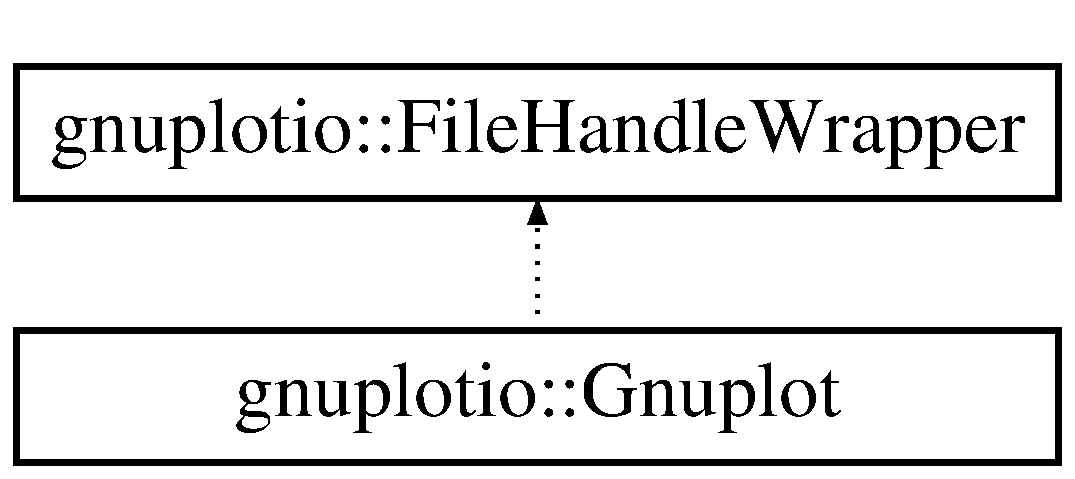
\includegraphics[height=2.000000cm]{structgnuplotio_1_1_file_handle_wrapper}
\end{center}
\end{figure}
\subsection*{Public Member Functions}
\begin{DoxyCompactItemize}
\item 
\hyperlink{structgnuplotio_1_1_file_handle_wrapper_a26b2378e193a9c41be5aed97e11f9411}{File\+Handle\+Wrapper} (std\+::\+F\+I\+LE $\ast$\+\_\+fh, bool \+\_\+should\+\_\+use\+\_\+pclose)
\item 
void \hyperlink{structgnuplotio_1_1_file_handle_wrapper_acafac45efd9c78ce621af4f3228c6f67}{fh\+\_\+close} ()
\item 
int \hyperlink{structgnuplotio_1_1_file_handle_wrapper_a3202ccd15d624f26dd2cf699d3456de6}{fh\+\_\+fileno} ()
\end{DoxyCompactItemize}
\subsection*{Public Attributes}
\begin{DoxyCompactItemize}
\item 
std\+::\+F\+I\+LE $\ast$ \hyperlink{structgnuplotio_1_1_file_handle_wrapper_adcb58bfcd9dbdba000a7e7395bee2ef9}{wrapped\+\_\+fh}
\item 
bool \hyperlink{structgnuplotio_1_1_file_handle_wrapper_a11b63ed64cf53167e26c5273778d90ea}{should\+\_\+use\+\_\+pclose}
\end{DoxyCompactItemize}


\subsection{Detailed Description}


Definition at line 1523 of file gnuplot-\/iostream.\+h.



\subsection{Constructor \& Destructor Documentation}
\index{gnuplotio\+::\+File\+Handle\+Wrapper@{gnuplotio\+::\+File\+Handle\+Wrapper}!File\+Handle\+Wrapper@{File\+Handle\+Wrapper}}
\index{File\+Handle\+Wrapper@{File\+Handle\+Wrapper}!gnuplotio\+::\+File\+Handle\+Wrapper@{gnuplotio\+::\+File\+Handle\+Wrapper}}
\subsubsection[{\texorpdfstring{File\+Handle\+Wrapper(std\+::\+F\+I\+L\+E $\ast$\+\_\+fh, bool \+\_\+should\+\_\+use\+\_\+pclose)}{FileHandleWrapper(std::FILE *_fh, bool _should_use_pclose)}}]{\setlength{\rightskip}{0pt plus 5cm}gnuplotio\+::\+File\+Handle\+Wrapper\+::\+File\+Handle\+Wrapper (
\begin{DoxyParamCaption}
\item[{std\+::\+F\+I\+LE $\ast$}]{\+\_\+fh, }
\item[{bool}]{\+\_\+should\+\_\+use\+\_\+pclose}
\end{DoxyParamCaption}
)\hspace{0.3cm}{\ttfamily [inline]}}\hypertarget{structgnuplotio_1_1_file_handle_wrapper_a26b2378e193a9c41be5aed97e11f9411}{}\label{structgnuplotio_1_1_file_handle_wrapper_a26b2378e193a9c41be5aed97e11f9411}


Definition at line 1524 of file gnuplot-\/iostream.\+h.



\subsection{Member Function Documentation}
\index{gnuplotio\+::\+File\+Handle\+Wrapper@{gnuplotio\+::\+File\+Handle\+Wrapper}!fh\+\_\+close@{fh\+\_\+close}}
\index{fh\+\_\+close@{fh\+\_\+close}!gnuplotio\+::\+File\+Handle\+Wrapper@{gnuplotio\+::\+File\+Handle\+Wrapper}}
\subsubsection[{\texorpdfstring{fh\+\_\+close()}{fh_close()}}]{\setlength{\rightskip}{0pt plus 5cm}void gnuplotio\+::\+File\+Handle\+Wrapper\+::fh\+\_\+close (
\begin{DoxyParamCaption}
{}
\end{DoxyParamCaption}
)\hspace{0.3cm}{\ttfamily [inline]}}\hypertarget{structgnuplotio_1_1_file_handle_wrapper_acafac45efd9c78ce621af4f3228c6f67}{}\label{structgnuplotio_1_1_file_handle_wrapper_acafac45efd9c78ce621af4f3228c6f67}


Definition at line 1527 of file gnuplot-\/iostream.\+h.

\index{gnuplotio\+::\+File\+Handle\+Wrapper@{gnuplotio\+::\+File\+Handle\+Wrapper}!fh\+\_\+fileno@{fh\+\_\+fileno}}
\index{fh\+\_\+fileno@{fh\+\_\+fileno}!gnuplotio\+::\+File\+Handle\+Wrapper@{gnuplotio\+::\+File\+Handle\+Wrapper}}
\subsubsection[{\texorpdfstring{fh\+\_\+fileno()}{fh_fileno()}}]{\setlength{\rightskip}{0pt plus 5cm}int gnuplotio\+::\+File\+Handle\+Wrapper\+::fh\+\_\+fileno (
\begin{DoxyParamCaption}
{}
\end{DoxyParamCaption}
)\hspace{0.3cm}{\ttfamily [inline]}}\hypertarget{structgnuplotio_1_1_file_handle_wrapper_a3202ccd15d624f26dd2cf699d3456de6}{}\label{structgnuplotio_1_1_file_handle_wrapper_a3202ccd15d624f26dd2cf699d3456de6}


Definition at line 1539 of file gnuplot-\/iostream.\+h.



\subsection{Member Data Documentation}
\index{gnuplotio\+::\+File\+Handle\+Wrapper@{gnuplotio\+::\+File\+Handle\+Wrapper}!should\+\_\+use\+\_\+pclose@{should\+\_\+use\+\_\+pclose}}
\index{should\+\_\+use\+\_\+pclose@{should\+\_\+use\+\_\+pclose}!gnuplotio\+::\+File\+Handle\+Wrapper@{gnuplotio\+::\+File\+Handle\+Wrapper}}
\subsubsection[{\texorpdfstring{should\+\_\+use\+\_\+pclose}{should_use_pclose}}]{\setlength{\rightskip}{0pt plus 5cm}bool gnuplotio\+::\+File\+Handle\+Wrapper\+::should\+\_\+use\+\_\+pclose}\hypertarget{structgnuplotio_1_1_file_handle_wrapper_a11b63ed64cf53167e26c5273778d90ea}{}\label{structgnuplotio_1_1_file_handle_wrapper_a11b63ed64cf53167e26c5273778d90ea}


Definition at line 1544 of file gnuplot-\/iostream.\+h.

\index{gnuplotio\+::\+File\+Handle\+Wrapper@{gnuplotio\+::\+File\+Handle\+Wrapper}!wrapped\+\_\+fh@{wrapped\+\_\+fh}}
\index{wrapped\+\_\+fh@{wrapped\+\_\+fh}!gnuplotio\+::\+File\+Handle\+Wrapper@{gnuplotio\+::\+File\+Handle\+Wrapper}}
\subsubsection[{\texorpdfstring{wrapped\+\_\+fh}{wrapped_fh}}]{\setlength{\rightskip}{0pt plus 5cm}std\+::\+F\+I\+LE$\ast$ gnuplotio\+::\+File\+Handle\+Wrapper\+::wrapped\+\_\+fh}\hypertarget{structgnuplotio_1_1_file_handle_wrapper_adcb58bfcd9dbdba000a7e7395bee2ef9}{}\label{structgnuplotio_1_1_file_handle_wrapper_adcb58bfcd9dbdba000a7e7395bee2ef9}


Definition at line 1543 of file gnuplot-\/iostream.\+h.



The documentation for this struct was generated from the following file\+:\begin{DoxyCompactItemize}
\item 
include/\hyperlink{gnuplot-iostream_8h}{gnuplot-\/iostream.\+h}\end{DoxyCompactItemize}

\hypertarget{structgnuplotio_1_1_flat_binary_sender}{}\section{gnuplotio\+:\+:Flat\+Binary\+Sender$<$ T $>$ Struct Template Reference}
\label{structgnuplotio_1_1_flat_binary_sender}\index{gnuplotio\+::\+Flat\+Binary\+Sender$<$ T $>$@{gnuplotio\+::\+Flat\+Binary\+Sender$<$ T $>$}}


{\ttfamily \#include $<$gnuplot-\/iostream.\+h$>$}

\subsection*{Static Public Member Functions}
\begin{DoxyCompactItemize}
\item 
static void \hyperlink{structgnuplotio_1_1_flat_binary_sender_a24d085492f2539c14033cd5c6ba75ba5}{send} (std\+::ostream \&stream, const T \&v)
\end{DoxyCompactItemize}


\subsection{Detailed Description}
\subsubsection*{template$<$typename T$>$\\*
struct gnuplotio\+::\+Flat\+Binary\+Sender$<$ T $>$}



Definition at line 451 of file gnuplot-\/iostream.\+h.



\subsection{Member Function Documentation}
\index{gnuplotio\+::\+Flat\+Binary\+Sender@{gnuplotio\+::\+Flat\+Binary\+Sender}!send@{send}}
\index{send@{send}!gnuplotio\+::\+Flat\+Binary\+Sender@{gnuplotio\+::\+Flat\+Binary\+Sender}}
\subsubsection[{\texorpdfstring{send(std\+::ostream \&stream, const T \&v)}{send(std::ostream &stream, const T &v)}}]{\setlength{\rightskip}{0pt plus 5cm}template$<$typename T$>$ static void {\bf gnuplotio\+::\+Flat\+Binary\+Sender}$<$ T $>$\+::send (
\begin{DoxyParamCaption}
\item[{std\+::ostream \&}]{stream, }
\item[{const T \&}]{v}
\end{DoxyParamCaption}
)\hspace{0.3cm}{\ttfamily [inline]}, {\ttfamily [static]}}\hypertarget{structgnuplotio_1_1_flat_binary_sender_a24d085492f2539c14033cd5c6ba75ba5}{}\label{structgnuplotio_1_1_flat_binary_sender_a24d085492f2539c14033cd5c6ba75ba5}


Definition at line 452 of file gnuplot-\/iostream.\+h.



The documentation for this struct was generated from the following file\+:\begin{DoxyCompactItemize}
\item 
include/\hyperlink{gnuplot-iostream_8h}{gnuplot-\/iostream.\+h}\end{DoxyCompactItemize}

\hypertarget{structgnuplotio_1_1_float_text_sender}{}\section{gnuplotio\+:\+:Float\+Text\+Sender$<$ T $>$ Struct Template Reference}
\label{structgnuplotio_1_1_float_text_sender}\index{gnuplotio\+::\+Float\+Text\+Sender$<$ T $>$@{gnuplotio\+::\+Float\+Text\+Sender$<$ T $>$}}


{\ttfamily \#include $<$gnuplot-\/iostream.\+h$>$}

\subsection*{Static Public Member Functions}
\begin{DoxyCompactItemize}
\item 
static void \hyperlink{structgnuplotio_1_1_float_text_sender_aed6b6c3a95b1396688800d6d1f2fc299}{send} (std\+::ostream \&stream, const T \&v)
\end{DoxyCompactItemize}


\subsection{Detailed Description}
\subsubsection*{template$<$typename T$>$\\*
struct gnuplotio\+::\+Float\+Text\+Sender$<$ T $>$}



Definition at line 505 of file gnuplot-\/iostream.\+h.



\subsection{Member Function Documentation}
\index{gnuplotio\+::\+Float\+Text\+Sender@{gnuplotio\+::\+Float\+Text\+Sender}!send@{send}}
\index{send@{send}!gnuplotio\+::\+Float\+Text\+Sender@{gnuplotio\+::\+Float\+Text\+Sender}}
\subsubsection[{\texorpdfstring{send(std\+::ostream \&stream, const T \&v)}{send(std::ostream &stream, const T &v)}}]{\setlength{\rightskip}{0pt plus 5cm}template$<$typename T$>$ static void {\bf gnuplotio\+::\+Float\+Text\+Sender}$<$ T $>$\+::send (
\begin{DoxyParamCaption}
\item[{std\+::ostream \&}]{stream, }
\item[{const T \&}]{v}
\end{DoxyParamCaption}
)\hspace{0.3cm}{\ttfamily [inline]}, {\ttfamily [static]}}\hypertarget{structgnuplotio_1_1_float_text_sender_aed6b6c3a95b1396688800d6d1f2fc299}{}\label{structgnuplotio_1_1_float_text_sender_aed6b6c3a95b1396688800d6d1f2fc299}


Definition at line 506 of file gnuplot-\/iostream.\+h.



The documentation for this struct was generated from the following file\+:\begin{DoxyCompactItemize}
\item 
include/\hyperlink{gnuplot-iostream_8h}{gnuplot-\/iostream.\+h}\end{DoxyCompactItemize}

\hypertarget{classgnuplotio_1_1_gnuplot}{}\section{gnuplotio\+:\+:Gnuplot Class Reference}
\label{classgnuplotio_1_1_gnuplot}\index{gnuplotio\+::\+Gnuplot@{gnuplotio\+::\+Gnuplot}}


{\ttfamily \#include $<$gnuplot-\/iostream.\+h$>$}

Inheritance diagram for gnuplotio\+:\+:Gnuplot\+:\begin{figure}[H]
\begin{center}
\leavevmode
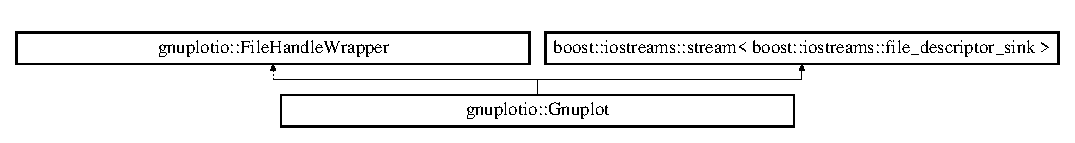
\includegraphics[height=1.469816cm]{classgnuplotio_1_1_gnuplot}
\end{center}
\end{figure}
\subsection*{Public Member Functions}
\begin{DoxyCompactItemize}
\item 
\hyperlink{classgnuplotio_1_1_gnuplot_ab2fb14389ab63ad5d9b2e57169bbbf1d}{Gnuplot} (const std\+::string \&\+\_\+cmd=\char`\"{}\char`\"{})
\item 
\hyperlink{classgnuplotio_1_1_gnuplot_a4a4f48a548e6ce6d485ca0a868410078}{Gnuplot} (F\+I\+LE $\ast$\+\_\+fh)
\item 
\hyperlink{classgnuplotio_1_1_gnuplot_ad10824df011e645542b5f97a903f4c31}{$\sim$\+Gnuplot} ()
\item 
void \hyperlink{classgnuplotio_1_1_gnuplot_a0d62f80988c3db4413a668e366406393}{clear\+Tmpfiles} ()
\item 
{\footnotesize template$<$typename T , typename Organization\+Mode $>$ }\\\hyperlink{classgnuplotio_1_1_gnuplot}{Gnuplot} \& \hyperlink{classgnuplotio_1_1_gnuplot_ae3f4c07960aa5601cc72158be67f945c}{send} (const T \&arg, Organization\+Mode)
\item 
{\footnotesize template$<$typename T , typename Organization\+Mode $>$ }\\\hyperlink{classgnuplotio_1_1_gnuplot}{Gnuplot} \& \hyperlink{classgnuplotio_1_1_gnuplot_a46c9e01d2030768cd811d2e8dbd10dfa}{send\+Binary} (const T \&arg, Organization\+Mode)
\item 
{\footnotesize template$<$typename T , typename Organization\+Mode $>$ }\\std\+::string \hyperlink{classgnuplotio_1_1_gnuplot_a43fe103649ec168b453c43aecdacce81}{binfmt} (const T \&arg, const std\+::string \&\hyperlink{classgnuplotio_1_1_gnuplot_a2d194dbd4d2f3475ff6f9b8384e62a9f}{arr\+\_\+or\+\_\+rec}, Organization\+Mode)
\item 
{\footnotesize template$<$typename T , typename Organization\+Mode $>$ }\\std\+::string \hyperlink{classgnuplotio_1_1_gnuplot_a9b9980e3b3d7cbb233a989e27468fa55}{file} (const T \&arg, std\+::string filename, Organization\+Mode)
\item 
{\footnotesize template$<$typename T , typename Organization\+Mode $>$ }\\std\+::string \hyperlink{classgnuplotio_1_1_gnuplot_ad90501e6dbab5379abcd76fd0e2e4ef1}{binary\+File} (const T \&arg, std\+::string filename, const std\+::string \&\hyperlink{classgnuplotio_1_1_gnuplot_a2d194dbd4d2f3475ff6f9b8384e62a9f}{arr\+\_\+or\+\_\+rec}, Organization\+Mode)
\item 
{\footnotesize template$<$typename T $>$ }\\\hyperlink{classgnuplotio_1_1_gnuplot}{Gnuplot} \hyperlink{classgnuplotio_1_1_gnuplot_ab2edc3c8f57483c6d9db86d685f3eee7}{G\+N\+U\+P\+L\+O\+T\+\_\+\+D\+E\+P\+R\+E\+C\+A\+TE} (\char`\"{}use send1d or send2d\char`\"{})\&send(const T \&arg)
\item 
{\footnotesize template$<$typename T $>$ }\\std\+::string \hyperlink{classgnuplotio_1_1_gnuplot_aeb3ba94ed04ecd46b55f89591ba23e7c}{G\+N\+U\+P\+L\+O\+T\+\_\+\+D\+E\+P\+R\+E\+C\+A\+TE} (\char`\"{}use binfmt1d or binfmt2d\char`\"{}) binfmt(const T \&arg
\end{DoxyCompactItemize}
\subsection*{Public Attributes}
\begin{DoxyCompactItemize}
\item 
std\+::string const std\+::string \& \hyperlink{classgnuplotio_1_1_gnuplot_a2d194dbd4d2f3475ff6f9b8384e62a9f}{arr\+\_\+or\+\_\+rec}
\item 
std\+::vector$<$ int $>$ \hyperlink{classgnuplotio_1_1_gnuplot_a92a4f6322e486de17db4507a5fc77348}{tmp\+\_\+files}
\item 
bool \hyperlink{classgnuplotio_1_1_gnuplot_a63e08bfd0cd02937d895ecfb6180107c}{debug\+\_\+messages}
\end{DoxyCompactItemize}


\subsection{Detailed Description}


Definition at line 1551 of file gnuplot-\/iostream.\+h.



\subsection{Constructor \& Destructor Documentation}
\index{gnuplotio\+::\+Gnuplot@{gnuplotio\+::\+Gnuplot}!Gnuplot@{Gnuplot}}
\index{Gnuplot@{Gnuplot}!gnuplotio\+::\+Gnuplot@{gnuplotio\+::\+Gnuplot}}
\subsubsection[{\texorpdfstring{Gnuplot(const std\+::string \&\+\_\+cmd="""")}{Gnuplot(const std::string &_cmd="")}}]{\setlength{\rightskip}{0pt plus 5cm}gnuplotio\+::\+Gnuplot\+::\+Gnuplot (
\begin{DoxyParamCaption}
\item[{const std\+::string \&}]{\+\_\+cmd = {\ttfamily \char`\"{}\char`\"{}}}
\end{DoxyParamCaption}
)\hspace{0.3cm}{\ttfamily [inline]}, {\ttfamily [explicit]}}\hypertarget{classgnuplotio_1_1_gnuplot_ab2fb14389ab63ad5d9b2e57169bbbf1d}{}\label{classgnuplotio_1_1_gnuplot_ab2fb14389ab63ad5d9b2e57169bbbf1d}


Definition at line 1588 of file gnuplot-\/iostream.\+h.

\index{gnuplotio\+::\+Gnuplot@{gnuplotio\+::\+Gnuplot}!Gnuplot@{Gnuplot}}
\index{Gnuplot@{Gnuplot}!gnuplotio\+::\+Gnuplot@{gnuplotio\+::\+Gnuplot}}
\subsubsection[{\texorpdfstring{Gnuplot(\+F\+I\+L\+E $\ast$\+\_\+fh)}{Gnuplot(FILE *_fh)}}]{\setlength{\rightskip}{0pt plus 5cm}gnuplotio\+::\+Gnuplot\+::\+Gnuplot (
\begin{DoxyParamCaption}
\item[{F\+I\+LE $\ast$}]{\+\_\+fh}
\end{DoxyParamCaption}
)\hspace{0.3cm}{\ttfamily [inline]}, {\ttfamily [explicit]}}\hypertarget{classgnuplotio_1_1_gnuplot_a4a4f48a548e6ce6d485ca0a868410078}{}\label{classgnuplotio_1_1_gnuplot_a4a4f48a548e6ce6d485ca0a868410078}


Definition at line 1605 of file gnuplot-\/iostream.\+h.

\index{gnuplotio\+::\+Gnuplot@{gnuplotio\+::\+Gnuplot}!````~Gnuplot@{$\sim$\+Gnuplot}}
\index{````~Gnuplot@{$\sim$\+Gnuplot}!gnuplotio\+::\+Gnuplot@{gnuplotio\+::\+Gnuplot}}
\subsubsection[{\texorpdfstring{$\sim$\+Gnuplot()}{~Gnuplot()}}]{\setlength{\rightskip}{0pt plus 5cm}gnuplotio\+::\+Gnuplot\+::$\sim$\+Gnuplot (
\begin{DoxyParamCaption}
{}
\end{DoxyParamCaption}
)\hspace{0.3cm}{\ttfamily [inline]}}\hypertarget{classgnuplotio_1_1_gnuplot_ad10824df011e645542b5f97a903f4c31}{}\label{classgnuplotio_1_1_gnuplot_ad10824df011e645542b5f97a903f4c31}


Definition at line 1628 of file gnuplot-\/iostream.\+h.



\subsection{Member Function Documentation}
\index{gnuplotio\+::\+Gnuplot@{gnuplotio\+::\+Gnuplot}!binary\+File@{binary\+File}}
\index{binary\+File@{binary\+File}!gnuplotio\+::\+Gnuplot@{gnuplotio\+::\+Gnuplot}}
\subsubsection[{\texorpdfstring{binary\+File(const T \&arg, std\+::string filename, const std\+::string \&arr\+\_\+or\+\_\+rec, Organization\+Mode)}{binaryFile(const T &arg, std::string filename, const std::string &arr_or_rec, OrganizationMode)}}]{\setlength{\rightskip}{0pt plus 5cm}template$<$typename T , typename Organization\+Mode $>$ std\+::string gnuplotio\+::\+Gnuplot\+::binary\+File (
\begin{DoxyParamCaption}
\item[{const T \&}]{arg, }
\item[{std\+::string}]{filename, }
\item[{const std\+::string \&}]{arr\+\_\+or\+\_\+rec, }
\item[{Organization\+Mode}]{}
\end{DoxyParamCaption}
)\hspace{0.3cm}{\ttfamily [inline]}}\hypertarget{classgnuplotio_1_1_gnuplot_ad90501e6dbab5379abcd76fd0e2e4ef1}{}\label{classgnuplotio_1_1_gnuplot_ad90501e6dbab5379abcd76fd0e2e4ef1}


Definition at line 1726 of file gnuplot-\/iostream.\+h.

\index{gnuplotio\+::\+Gnuplot@{gnuplotio\+::\+Gnuplot}!binfmt@{binfmt}}
\index{binfmt@{binfmt}!gnuplotio\+::\+Gnuplot@{gnuplotio\+::\+Gnuplot}}
\subsubsection[{\texorpdfstring{binfmt(const T \&arg, const std\+::string \&arr\+\_\+or\+\_\+rec, Organization\+Mode)}{binfmt(const T &arg, const std::string &arr_or_rec, OrganizationMode)}}]{\setlength{\rightskip}{0pt plus 5cm}template$<$typename T , typename Organization\+Mode $>$ std\+::string gnuplotio\+::\+Gnuplot\+::binfmt (
\begin{DoxyParamCaption}
\item[{const T \&}]{arg, }
\item[{const std\+::string \&}]{arr\+\_\+or\+\_\+rec, }
\item[{Organization\+Mode}]{}
\end{DoxyParamCaption}
)\hspace{0.3cm}{\ttfamily [inline]}}\hypertarget{classgnuplotio_1_1_gnuplot_a43fe103649ec168b453c43aecdacce81}{}\label{classgnuplotio_1_1_gnuplot_a43fe103649ec168b453c43aecdacce81}


Definition at line 1691 of file gnuplot-\/iostream.\+h.

\index{gnuplotio\+::\+Gnuplot@{gnuplotio\+::\+Gnuplot}!clear\+Tmpfiles@{clear\+Tmpfiles}}
\index{clear\+Tmpfiles@{clear\+Tmpfiles}!gnuplotio\+::\+Gnuplot@{gnuplotio\+::\+Gnuplot}}
\subsubsection[{\texorpdfstring{clear\+Tmpfiles()}{clearTmpfiles()}}]{\setlength{\rightskip}{0pt plus 5cm}void gnuplotio\+::\+Gnuplot\+::clear\+Tmpfiles (
\begin{DoxyParamCaption}
{}
\end{DoxyParamCaption}
)\hspace{0.3cm}{\ttfamily [inline]}}\hypertarget{classgnuplotio_1_1_gnuplot_a0d62f80988c3db4413a668e366406393}{}\label{classgnuplotio_1_1_gnuplot_a0d62f80988c3db4413a668e366406393}


Definition at line 1645 of file gnuplot-\/iostream.\+h.

\index{gnuplotio\+::\+Gnuplot@{gnuplotio\+::\+Gnuplot}!file@{file}}
\index{file@{file}!gnuplotio\+::\+Gnuplot@{gnuplotio\+::\+Gnuplot}}
\subsubsection[{\texorpdfstring{file(const T \&arg, std\+::string filename, Organization\+Mode)}{file(const T &arg, std::string filename, OrganizationMode)}}]{\setlength{\rightskip}{0pt plus 5cm}template$<$typename T , typename Organization\+Mode $>$ std\+::string gnuplotio\+::\+Gnuplot\+::file (
\begin{DoxyParamCaption}
\item[{const T \&}]{arg, }
\item[{std\+::string}]{filename, }
\item[{Organization\+Mode}]{}
\end{DoxyParamCaption}
)\hspace{0.3cm}{\ttfamily [inline]}}\hypertarget{classgnuplotio_1_1_gnuplot_a9b9980e3b3d7cbb233a989e27468fa55}{}\label{classgnuplotio_1_1_gnuplot_a9b9980e3b3d7cbb233a989e27468fa55}


Definition at line 1711 of file gnuplot-\/iostream.\+h.

\index{gnuplotio\+::\+Gnuplot@{gnuplotio\+::\+Gnuplot}!G\+N\+U\+P\+L\+O\+T\+\_\+\+D\+E\+P\+R\+E\+C\+A\+TE@{G\+N\+U\+P\+L\+O\+T\+\_\+\+D\+E\+P\+R\+E\+C\+A\+TE}}
\index{G\+N\+U\+P\+L\+O\+T\+\_\+\+D\+E\+P\+R\+E\+C\+A\+TE@{G\+N\+U\+P\+L\+O\+T\+\_\+\+D\+E\+P\+R\+E\+C\+A\+TE}!gnuplotio\+::\+Gnuplot@{gnuplotio\+::\+Gnuplot}}
\subsubsection[{\texorpdfstring{G\+N\+U\+P\+L\+O\+T\+\_\+\+D\+E\+P\+R\+E\+C\+A\+T\+E(""use send1d or send2d"")\&send(const T \&arg)}{GNUPLOT_DEPRECATE("use send1d or send2d")&send(const T &arg)}}]{\setlength{\rightskip}{0pt plus 5cm}template$<$typename T $>$ {\bf Gnuplot} gnuplotio\+::\+Gnuplot\+::\+G\+N\+U\+P\+L\+O\+T\+\_\+\+D\+E\+P\+R\+E\+C\+A\+TE (
\begin{DoxyParamCaption}
\item[{\char`\"{}use send1d or send2d\char`\"{}}]{}
\end{DoxyParamCaption}
) const\hspace{0.3cm}{\ttfamily [inline]}}\hypertarget{classgnuplotio_1_1_gnuplot_ab2edc3c8f57483c6d9db86d685f3eee7}{}\label{classgnuplotio_1_1_gnuplot_ab2edc3c8f57483c6d9db86d685f3eee7}


Definition at line 1744 of file gnuplot-\/iostream.\+h.

\index{gnuplotio\+::\+Gnuplot@{gnuplotio\+::\+Gnuplot}!G\+N\+U\+P\+L\+O\+T\+\_\+\+D\+E\+P\+R\+E\+C\+A\+TE@{G\+N\+U\+P\+L\+O\+T\+\_\+\+D\+E\+P\+R\+E\+C\+A\+TE}}
\index{G\+N\+U\+P\+L\+O\+T\+\_\+\+D\+E\+P\+R\+E\+C\+A\+TE@{G\+N\+U\+P\+L\+O\+T\+\_\+\+D\+E\+P\+R\+E\+C\+A\+TE}!gnuplotio\+::\+Gnuplot@{gnuplotio\+::\+Gnuplot}}
\subsubsection[{\texorpdfstring{G\+N\+U\+P\+L\+O\+T\+\_\+\+D\+E\+P\+R\+E\+C\+A\+T\+E(""use binfmt1d or binfmt2d"") binfmt(const T \&arg}{GNUPLOT_DEPRECATE("use binfmt1d or binfmt2d") binfmt(const T &arg}}]{\setlength{\rightskip}{0pt plus 5cm}template$<$typename T $>$ std\+::string gnuplotio\+::\+Gnuplot\+::\+G\+N\+U\+P\+L\+O\+T\+\_\+\+D\+E\+P\+R\+E\+C\+A\+TE (
\begin{DoxyParamCaption}
\item[{\char`\"{}use binfmt1d or binfmt2d\char`\"{}}]{}
\end{DoxyParamCaption}
) const}\hypertarget{classgnuplotio_1_1_gnuplot_aeb3ba94ed04ecd46b55f89591ba23e7c}{}\label{classgnuplotio_1_1_gnuplot_aeb3ba94ed04ecd46b55f89591ba23e7c}
\index{gnuplotio\+::\+Gnuplot@{gnuplotio\+::\+Gnuplot}!send@{send}}
\index{send@{send}!gnuplotio\+::\+Gnuplot@{gnuplotio\+::\+Gnuplot}}
\subsubsection[{\texorpdfstring{send(const T \&arg, Organization\+Mode)}{send(const T &arg, OrganizationMode)}}]{\setlength{\rightskip}{0pt plus 5cm}template$<$typename T , typename Organization\+Mode $>$ {\bf Gnuplot}\& gnuplotio\+::\+Gnuplot\+::send (
\begin{DoxyParamCaption}
\item[{const T \&}]{arg, }
\item[{Organization\+Mode}]{}
\end{DoxyParamCaption}
)\hspace{0.3cm}{\ttfamily [inline]}}\hypertarget{classgnuplotio_1_1_gnuplot_ae3f4c07960aa5601cc72158be67f945c}{}\label{classgnuplotio_1_1_gnuplot_ae3f4c07960aa5601cc72158be67f945c}


Definition at line 1676 of file gnuplot-\/iostream.\+h.

\index{gnuplotio\+::\+Gnuplot@{gnuplotio\+::\+Gnuplot}!send\+Binary@{send\+Binary}}
\index{send\+Binary@{send\+Binary}!gnuplotio\+::\+Gnuplot@{gnuplotio\+::\+Gnuplot}}
\subsubsection[{\texorpdfstring{send\+Binary(const T \&arg, Organization\+Mode)}{sendBinary(const T &arg, OrganizationMode)}}]{\setlength{\rightskip}{0pt plus 5cm}template$<$typename T , typename Organization\+Mode $>$ {\bf Gnuplot}\& gnuplotio\+::\+Gnuplot\+::send\+Binary (
\begin{DoxyParamCaption}
\item[{const T \&}]{arg, }
\item[{Organization\+Mode}]{}
\end{DoxyParamCaption}
)\hspace{0.3cm}{\ttfamily [inline]}}\hypertarget{classgnuplotio_1_1_gnuplot_a46c9e01d2030768cd811d2e8dbd10dfa}{}\label{classgnuplotio_1_1_gnuplot_a46c9e01d2030768cd811d2e8dbd10dfa}


Definition at line 1684 of file gnuplot-\/iostream.\+h.



\subsection{Member Data Documentation}
\index{gnuplotio\+::\+Gnuplot@{gnuplotio\+::\+Gnuplot}!arr\+\_\+or\+\_\+rec@{arr\+\_\+or\+\_\+rec}}
\index{arr\+\_\+or\+\_\+rec@{arr\+\_\+or\+\_\+rec}!gnuplotio\+::\+Gnuplot@{gnuplotio\+::\+Gnuplot}}
\subsubsection[{\texorpdfstring{arr\+\_\+or\+\_\+rec}{arr_or_rec}}]{\setlength{\rightskip}{0pt plus 5cm}std\+::string const std\+::string\& gnuplotio\+::\+Gnuplot\+::arr\+\_\+or\+\_\+rec}\hypertarget{classgnuplotio_1_1_gnuplot_a2d194dbd4d2f3475ff6f9b8384e62a9f}{}\label{classgnuplotio_1_1_gnuplot_a2d194dbd4d2f3475ff6f9b8384e62a9f}


Definition at line 1748 of file gnuplot-\/iostream.\+h.

\index{gnuplotio\+::\+Gnuplot@{gnuplotio\+::\+Gnuplot}!debug\+\_\+messages@{debug\+\_\+messages}}
\index{debug\+\_\+messages@{debug\+\_\+messages}!gnuplotio\+::\+Gnuplot@{gnuplotio\+::\+Gnuplot}}
\subsubsection[{\texorpdfstring{debug\+\_\+messages}{debug_messages}}]{\setlength{\rightskip}{0pt plus 5cm}bool gnuplotio\+::\+Gnuplot\+::debug\+\_\+messages}\hypertarget{classgnuplotio_1_1_gnuplot_a63e08bfd0cd02937d895ecfb6180107c}{}\label{classgnuplotio_1_1_gnuplot_a63e08bfd0cd02937d895ecfb6180107c}


Definition at line 1849 of file gnuplot-\/iostream.\+h.

\index{gnuplotio\+::\+Gnuplot@{gnuplotio\+::\+Gnuplot}!tmp\+\_\+files@{tmp\+\_\+files}}
\index{tmp\+\_\+files@{tmp\+\_\+files}!gnuplotio\+::\+Gnuplot@{gnuplotio\+::\+Gnuplot}}
\subsubsection[{\texorpdfstring{tmp\+\_\+files}{tmp_files}}]{\setlength{\rightskip}{0pt plus 5cm}std\+::vector$<$int$>$ gnuplotio\+::\+Gnuplot\+::tmp\+\_\+files}\hypertarget{classgnuplotio_1_1_gnuplot_a92a4f6322e486de17db4507a5fc77348}{}\label{classgnuplotio_1_1_gnuplot_a92a4f6322e486de17db4507a5fc77348}


Definition at line 1845 of file gnuplot-\/iostream.\+h.



The documentation for this class was generated from the following file\+:\begin{DoxyCompactItemize}
\item 
include/\hyperlink{gnuplot-iostream_8h}{gnuplot-\/iostream.\+h}\end{DoxyCompactItemize}

\hypertarget{classgnuplotio_1_1_gnuplot_feedback}{}\section{gnuplotio\+:\+:Gnuplot\+Feedback Class Reference}
\label{classgnuplotio_1_1_gnuplot_feedback}\index{gnuplotio\+::\+Gnuplot\+Feedback@{gnuplotio\+::\+Gnuplot\+Feedback}}


{\ttfamily \#include $<$gnuplot-\/iostream.\+h$>$}

\subsection*{Public Member Functions}
\begin{DoxyCompactItemize}
\item 
\hyperlink{classgnuplotio_1_1_gnuplot_feedback_ad03d9a9fde314af659f260adc60b8583}{Gnuplot\+Feedback} ()
\item 
virtual \hyperlink{classgnuplotio_1_1_gnuplot_feedback_aad7d8173d2cef257c42dea7e5b5d2aaf}{$\sim$\+Gnuplot\+Feedback} ()
\item 
virtual std\+::string \hyperlink{classgnuplotio_1_1_gnuplot_feedback_a081d4d59ffd81e2322c07c0a802e1307}{filename} () const =0
\item 
virtual F\+I\+LE $\ast$ \hyperlink{classgnuplotio_1_1_gnuplot_feedback_a13ae87ba489bfbe87f64b8b54e8a4563}{handle} () const =0
\end{DoxyCompactItemize}


\subsection{Detailed Description}


Definition at line 290 of file gnuplot-\/iostream.\+h.



\subsection{Constructor \& Destructor Documentation}
\index{gnuplotio\+::\+Gnuplot\+Feedback@{gnuplotio\+::\+Gnuplot\+Feedback}!Gnuplot\+Feedback@{Gnuplot\+Feedback}}
\index{Gnuplot\+Feedback@{Gnuplot\+Feedback}!gnuplotio\+::\+Gnuplot\+Feedback@{gnuplotio\+::\+Gnuplot\+Feedback}}
\subsubsection[{\texorpdfstring{Gnuplot\+Feedback()}{GnuplotFeedback()}}]{\setlength{\rightskip}{0pt plus 5cm}gnuplotio\+::\+Gnuplot\+Feedback\+::\+Gnuplot\+Feedback (
\begin{DoxyParamCaption}
{}
\end{DoxyParamCaption}
)\hspace{0.3cm}{\ttfamily [inline]}}\hypertarget{classgnuplotio_1_1_gnuplot_feedback_ad03d9a9fde314af659f260adc60b8583}{}\label{classgnuplotio_1_1_gnuplot_feedback_ad03d9a9fde314af659f260adc60b8583}


Definition at line 292 of file gnuplot-\/iostream.\+h.

\index{gnuplotio\+::\+Gnuplot\+Feedback@{gnuplotio\+::\+Gnuplot\+Feedback}!````~Gnuplot\+Feedback@{$\sim$\+Gnuplot\+Feedback}}
\index{````~Gnuplot\+Feedback@{$\sim$\+Gnuplot\+Feedback}!gnuplotio\+::\+Gnuplot\+Feedback@{gnuplotio\+::\+Gnuplot\+Feedback}}
\subsubsection[{\texorpdfstring{$\sim$\+Gnuplot\+Feedback()}{~GnuplotFeedback()}}]{\setlength{\rightskip}{0pt plus 5cm}virtual gnuplotio\+::\+Gnuplot\+Feedback\+::$\sim$\+Gnuplot\+Feedback (
\begin{DoxyParamCaption}
{}
\end{DoxyParamCaption}
)\hspace{0.3cm}{\ttfamily [inline]}, {\ttfamily [virtual]}}\hypertarget{classgnuplotio_1_1_gnuplot_feedback_aad7d8173d2cef257c42dea7e5b5d2aaf}{}\label{classgnuplotio_1_1_gnuplot_feedback_aad7d8173d2cef257c42dea7e5b5d2aaf}


Definition at line 293 of file gnuplot-\/iostream.\+h.



\subsection{Member Function Documentation}
\index{gnuplotio\+::\+Gnuplot\+Feedback@{gnuplotio\+::\+Gnuplot\+Feedback}!filename@{filename}}
\index{filename@{filename}!gnuplotio\+::\+Gnuplot\+Feedback@{gnuplotio\+::\+Gnuplot\+Feedback}}
\subsubsection[{\texorpdfstring{filename() const =0}{filename() const =0}}]{\setlength{\rightskip}{0pt plus 5cm}virtual std\+::string gnuplotio\+::\+Gnuplot\+Feedback\+::filename (
\begin{DoxyParamCaption}
{}
\end{DoxyParamCaption}
) const\hspace{0.3cm}{\ttfamily [pure virtual]}}\hypertarget{classgnuplotio_1_1_gnuplot_feedback_a081d4d59ffd81e2322c07c0a802e1307}{}\label{classgnuplotio_1_1_gnuplot_feedback_a081d4d59ffd81e2322c07c0a802e1307}
\index{gnuplotio\+::\+Gnuplot\+Feedback@{gnuplotio\+::\+Gnuplot\+Feedback}!handle@{handle}}
\index{handle@{handle}!gnuplotio\+::\+Gnuplot\+Feedback@{gnuplotio\+::\+Gnuplot\+Feedback}}
\subsubsection[{\texorpdfstring{handle() const =0}{handle() const =0}}]{\setlength{\rightskip}{0pt plus 5cm}virtual F\+I\+LE$\ast$ gnuplotio\+::\+Gnuplot\+Feedback\+::handle (
\begin{DoxyParamCaption}
{}
\end{DoxyParamCaption}
) const\hspace{0.3cm}{\ttfamily [pure virtual]}}\hypertarget{classgnuplotio_1_1_gnuplot_feedback_a13ae87ba489bfbe87f64b8b54e8a4563}{}\label{classgnuplotio_1_1_gnuplot_feedback_a13ae87ba489bfbe87f64b8b54e8a4563}


The documentation for this class was generated from the following file\+:\begin{DoxyCompactItemize}
\item 
include/\hyperlink{gnuplot-iostream_8h}{gnuplot-\/iostream.\+h}\end{DoxyCompactItemize}

\hypertarget{structgnuplotio_1_1is__boost__tuple}{}\section{gnuplotio\+:\+:is\+\_\+boost\+\_\+tuple$<$ T $>$ Struct Template Reference}
\label{structgnuplotio_1_1is__boost__tuple}\index{gnuplotio\+::is\+\_\+boost\+\_\+tuple$<$ T $>$@{gnuplotio\+::is\+\_\+boost\+\_\+tuple$<$ T $>$}}


{\ttfamily \#include $<$gnuplot-\/iostream.\+h$>$}

\subsection*{Public Types}
\begin{DoxyCompactItemize}
\item 
typedef boost\+::mpl\+::and\+\_\+$<$ typename has\+\_\+head\+\_\+type$<$ T $>$\+::\hyperlink{structgnuplotio_1_1is__boost__tuple_ad771f62833b23ecae5dc689e6248396a}{type}, typename has\+\_\+tail\+\_\+type$<$ T $>$\+::\hyperlink{structgnuplotio_1_1is__boost__tuple_ad771f62833b23ecae5dc689e6248396a}{type} $>$ \hyperlink{structgnuplotio_1_1is__boost__tuple_ad771f62833b23ecae5dc689e6248396a}{type}
\end{DoxyCompactItemize}
\subsection*{Static Public Attributes}
\begin{DoxyCompactItemize}
\item 
static const bool \hyperlink{structgnuplotio_1_1is__boost__tuple_ae6664b02421d28585204104af65a4744}{value} = type\+::value
\end{DoxyCompactItemize}


\subsection{Detailed Description}
\subsubsection*{template$<$typename T$>$\\*
struct gnuplotio\+::is\+\_\+boost\+\_\+tuple$<$ T $>$}



Definition at line 213 of file gnuplot-\/iostream.\+h.



\subsection{Member Typedef Documentation}
\index{gnuplotio\+::is\+\_\+boost\+\_\+tuple@{gnuplotio\+::is\+\_\+boost\+\_\+tuple}!type@{type}}
\index{type@{type}!gnuplotio\+::is\+\_\+boost\+\_\+tuple@{gnuplotio\+::is\+\_\+boost\+\_\+tuple}}
\subsubsection[{\texorpdfstring{type}{type}}]{\setlength{\rightskip}{0pt plus 5cm}template$<$typename T $>$ typedef boost\+::mpl\+::and\+\_\+$<$ typename has\+\_\+head\+\_\+type$<$T$>$\+::{\bf type}, typename has\+\_\+tail\+\_\+type$<$T$>$\+::{\bf type} $>$ {\bf gnuplotio\+::is\+\_\+boost\+\_\+tuple}$<$ T $>$\+::{\bf type}}\hypertarget{structgnuplotio_1_1is__boost__tuple_ad771f62833b23ecae5dc689e6248396a}{}\label{structgnuplotio_1_1is__boost__tuple_ad771f62833b23ecae5dc689e6248396a}


Definition at line 217 of file gnuplot-\/iostream.\+h.



\subsection{Member Data Documentation}
\index{gnuplotio\+::is\+\_\+boost\+\_\+tuple@{gnuplotio\+::is\+\_\+boost\+\_\+tuple}!value@{value}}
\index{value@{value}!gnuplotio\+::is\+\_\+boost\+\_\+tuple@{gnuplotio\+::is\+\_\+boost\+\_\+tuple}}
\subsubsection[{\texorpdfstring{value}{value}}]{\setlength{\rightskip}{0pt plus 5cm}template$<$typename T $>$ const bool {\bf gnuplotio\+::is\+\_\+boost\+\_\+tuple}$<$ T $>$\+::value = type\+::value\hspace{0.3cm}{\ttfamily [static]}}\hypertarget{structgnuplotio_1_1is__boost__tuple_ae6664b02421d28585204104af65a4744}{}\label{structgnuplotio_1_1is__boost__tuple_ae6664b02421d28585204104af65a4744}


Definition at line 218 of file gnuplot-\/iostream.\+h.



The documentation for this struct was generated from the following file\+:\begin{DoxyCompactItemize}
\item 
include/\hyperlink{gnuplot-iostream_8h}{gnuplot-\/iostream.\+h}\end{DoxyCompactItemize}

\hypertarget{structgnuplotio_1_1is__boost__tuple__nulltype}{}\section{gnuplotio\+:\+:is\+\_\+boost\+\_\+tuple\+\_\+nulltype$<$ T $>$ Struct Template Reference}
\label{structgnuplotio_1_1is__boost__tuple__nulltype}\index{gnuplotio\+::is\+\_\+boost\+\_\+tuple\+\_\+nulltype$<$ T $>$@{gnuplotio\+::is\+\_\+boost\+\_\+tuple\+\_\+nulltype$<$ T $>$}}


{\ttfamily \#include $<$gnuplot-\/iostream.\+h$>$}

\subsection*{Public Types}
\begin{DoxyCompactItemize}
\item 
typedef boost\+::mpl\+::bool\+\_\+$<$ \hyperlink{structgnuplotio_1_1is__boost__tuple__nulltype_aed42a98e58eb94c7ba55ea7d2a8f7fd2}{value} $>$ \hyperlink{structgnuplotio_1_1is__boost__tuple__nulltype_a6b9e2eaadcaa5c788131d4e9e4186349}{type}
\end{DoxyCompactItemize}
\subsection*{Static Public Attributes}
\begin{DoxyCompactItemize}
\item 
static const bool \hyperlink{structgnuplotio_1_1is__boost__tuple__nulltype_aed42a98e58eb94c7ba55ea7d2a8f7fd2}{value} = false
\end{DoxyCompactItemize}


\subsection{Detailed Description}
\subsubsection*{template$<$typename T$>$\\*
struct gnuplotio\+::is\+\_\+boost\+\_\+tuple\+\_\+nulltype$<$ T $>$}



Definition at line 198 of file gnuplot-\/iostream.\+h.



\subsection{Member Typedef Documentation}
\index{gnuplotio\+::is\+\_\+boost\+\_\+tuple\+\_\+nulltype@{gnuplotio\+::is\+\_\+boost\+\_\+tuple\+\_\+nulltype}!type@{type}}
\index{type@{type}!gnuplotio\+::is\+\_\+boost\+\_\+tuple\+\_\+nulltype@{gnuplotio\+::is\+\_\+boost\+\_\+tuple\+\_\+nulltype}}
\subsubsection[{\texorpdfstring{type}{type}}]{\setlength{\rightskip}{0pt plus 5cm}template$<$typename T $>$ typedef boost\+::mpl\+::bool\+\_\+$<${\bf value}$>$ {\bf gnuplotio\+::is\+\_\+boost\+\_\+tuple\+\_\+nulltype}$<$ T $>$\+::{\bf type}}\hypertarget{structgnuplotio_1_1is__boost__tuple__nulltype_a6b9e2eaadcaa5c788131d4e9e4186349}{}\label{structgnuplotio_1_1is__boost__tuple__nulltype_a6b9e2eaadcaa5c788131d4e9e4186349}


Definition at line 200 of file gnuplot-\/iostream.\+h.



\subsection{Member Data Documentation}
\index{gnuplotio\+::is\+\_\+boost\+\_\+tuple\+\_\+nulltype@{gnuplotio\+::is\+\_\+boost\+\_\+tuple\+\_\+nulltype}!value@{value}}
\index{value@{value}!gnuplotio\+::is\+\_\+boost\+\_\+tuple\+\_\+nulltype@{gnuplotio\+::is\+\_\+boost\+\_\+tuple\+\_\+nulltype}}
\subsubsection[{\texorpdfstring{value}{value}}]{\setlength{\rightskip}{0pt plus 5cm}template$<$typename T $>$ const bool {\bf gnuplotio\+::is\+\_\+boost\+\_\+tuple\+\_\+nulltype}$<$ T $>$\+::value = false\hspace{0.3cm}{\ttfamily [static]}}\hypertarget{structgnuplotio_1_1is__boost__tuple__nulltype_aed42a98e58eb94c7ba55ea7d2a8f7fd2}{}\label{structgnuplotio_1_1is__boost__tuple__nulltype_aed42a98e58eb94c7ba55ea7d2a8f7fd2}


Definition at line 199 of file gnuplot-\/iostream.\+h.



The documentation for this struct was generated from the following file\+:\begin{DoxyCompactItemize}
\item 
include/\hyperlink{gnuplot-iostream_8h}{gnuplot-\/iostream.\+h}\end{DoxyCompactItemize}

\hypertarget{structgnuplotio_1_1is__boost__tuple__nulltype_3_01boost_1_1tuples_1_1null__type_01_4}{}\section{gnuplotio\+:\+:is\+\_\+boost\+\_\+tuple\+\_\+nulltype$<$ boost\+:\+:tuples\+:\+:null\+\_\+type $>$ Struct Template Reference}
\label{structgnuplotio_1_1is__boost__tuple__nulltype_3_01boost_1_1tuples_1_1null__type_01_4}\index{gnuplotio\+::is\+\_\+boost\+\_\+tuple\+\_\+nulltype$<$ boost\+::tuples\+::null\+\_\+type $>$@{gnuplotio\+::is\+\_\+boost\+\_\+tuple\+\_\+nulltype$<$ boost\+::tuples\+::null\+\_\+type $>$}}


{\ttfamily \#include $<$gnuplot-\/iostream.\+h$>$}

\subsection*{Public Types}
\begin{DoxyCompactItemize}
\item 
typedef boost\+::mpl\+::bool\+\_\+$<$ \hyperlink{structgnuplotio_1_1is__boost__tuple__nulltype_3_01boost_1_1tuples_1_1null__type_01_4_ae7fc5c63a7b01851c7ce12dbf634cfea}{value} $>$ \hyperlink{structgnuplotio_1_1is__boost__tuple__nulltype_3_01boost_1_1tuples_1_1null__type_01_4_aab5c47dbae2148f1e9ed4d89f25f21fd}{type}
\end{DoxyCompactItemize}
\subsection*{Static Public Attributes}
\begin{DoxyCompactItemize}
\item 
static const bool \hyperlink{structgnuplotio_1_1is__boost__tuple__nulltype_3_01boost_1_1tuples_1_1null__type_01_4_ae7fc5c63a7b01851c7ce12dbf634cfea}{value} = true
\end{DoxyCompactItemize}


\subsection{Detailed Description}
\subsubsection*{template$<$$>$\\*
struct gnuplotio\+::is\+\_\+boost\+\_\+tuple\+\_\+nulltype$<$ boost\+::tuples\+::null\+\_\+type $>$}



Definition at line 204 of file gnuplot-\/iostream.\+h.



\subsection{Member Typedef Documentation}
\index{gnuplotio\+::is\+\_\+boost\+\_\+tuple\+\_\+nulltype$<$ boost\+::tuples\+::null\+\_\+type $>$@{gnuplotio\+::is\+\_\+boost\+\_\+tuple\+\_\+nulltype$<$ boost\+::tuples\+::null\+\_\+type $>$}!type@{type}}
\index{type@{type}!gnuplotio\+::is\+\_\+boost\+\_\+tuple\+\_\+nulltype$<$ boost\+::tuples\+::null\+\_\+type $>$@{gnuplotio\+::is\+\_\+boost\+\_\+tuple\+\_\+nulltype$<$ boost\+::tuples\+::null\+\_\+type $>$}}
\subsubsection[{\texorpdfstring{type}{type}}]{\setlength{\rightskip}{0pt plus 5cm}typedef boost\+::mpl\+::bool\+\_\+$<${\bf value}$>$ {\bf gnuplotio\+::is\+\_\+boost\+\_\+tuple\+\_\+nulltype}$<$ boost\+::tuples\+::null\+\_\+type $>$\+::{\bf type}}\hypertarget{structgnuplotio_1_1is__boost__tuple__nulltype_3_01boost_1_1tuples_1_1null__type_01_4_aab5c47dbae2148f1e9ed4d89f25f21fd}{}\label{structgnuplotio_1_1is__boost__tuple__nulltype_3_01boost_1_1tuples_1_1null__type_01_4_aab5c47dbae2148f1e9ed4d89f25f21fd}


Definition at line 206 of file gnuplot-\/iostream.\+h.



\subsection{Member Data Documentation}
\index{gnuplotio\+::is\+\_\+boost\+\_\+tuple\+\_\+nulltype$<$ boost\+::tuples\+::null\+\_\+type $>$@{gnuplotio\+::is\+\_\+boost\+\_\+tuple\+\_\+nulltype$<$ boost\+::tuples\+::null\+\_\+type $>$}!value@{value}}
\index{value@{value}!gnuplotio\+::is\+\_\+boost\+\_\+tuple\+\_\+nulltype$<$ boost\+::tuples\+::null\+\_\+type $>$@{gnuplotio\+::is\+\_\+boost\+\_\+tuple\+\_\+nulltype$<$ boost\+::tuples\+::null\+\_\+type $>$}}
\subsubsection[{\texorpdfstring{value}{value}}]{\setlength{\rightskip}{0pt plus 5cm}const bool {\bf gnuplotio\+::is\+\_\+boost\+\_\+tuple\+\_\+nulltype}$<$ boost\+::tuples\+::null\+\_\+type $>$\+::value = true\hspace{0.3cm}{\ttfamily [static]}}\hypertarget{structgnuplotio_1_1is__boost__tuple__nulltype_3_01boost_1_1tuples_1_1null__type_01_4_ae7fc5c63a7b01851c7ce12dbf634cfea}{}\label{structgnuplotio_1_1is__boost__tuple__nulltype_3_01boost_1_1tuples_1_1null__type_01_4_ae7fc5c63a7b01851c7ce12dbf634cfea}


Definition at line 205 of file gnuplot-\/iostream.\+h.



The documentation for this struct was generated from the following file\+:\begin{DoxyCompactItemize}
\item 
include/\hyperlink{gnuplot-iostream_8h}{gnuplot-\/iostream.\+h}\end{DoxyCompactItemize}

\hypertarget{structgnuplotio_1_1is__like__stl__container}{}\section{gnuplotio\+:\+:is\+\_\+like\+\_\+stl\+\_\+container$<$ T $>$ Struct Template Reference}
\label{structgnuplotio_1_1is__like__stl__container}\index{gnuplotio\+::is\+\_\+like\+\_\+stl\+\_\+container$<$ T $>$@{gnuplotio\+::is\+\_\+like\+\_\+stl\+\_\+container$<$ T $>$}}


{\ttfamily \#include $<$gnuplot-\/iostream.\+h$>$}

\subsection*{Public Types}
\begin{DoxyCompactItemize}
\item 
typedef boost\+::mpl\+::and\+\_\+$<$ typename has\+\_\+value\+\_\+type$<$ T $>$\+::\hyperlink{structgnuplotio_1_1is__like__stl__container_a050ecfa55e896a27f86d901334f47c6a}{type}, typename has\+\_\+const\+\_\+iterator$<$ T $>$\+::\hyperlink{structgnuplotio_1_1is__like__stl__container_a050ecfa55e896a27f86d901334f47c6a}{type}, boost\+::mpl\+::not\+\_\+$<$ \hyperlink{structgnuplotio_1_1dont__treat__as__stl__container}{dont\+\_\+treat\+\_\+as\+\_\+stl\+\_\+container}$<$ T $>$ $>$ $>$ \hyperlink{structgnuplotio_1_1is__like__stl__container_a050ecfa55e896a27f86d901334f47c6a}{type}
\end{DoxyCompactItemize}
\subsection*{Static Public Attributes}
\begin{DoxyCompactItemize}
\item 
static const bool \hyperlink{structgnuplotio_1_1is__like__stl__container_ae4761e6e807deed732e41118c785c8a4}{value} = type\+::value
\end{DoxyCompactItemize}


\subsection{Detailed Description}
\subsubsection*{template$<$typename T$>$\\*
struct gnuplotio\+::is\+\_\+like\+\_\+stl\+\_\+container$<$ T $>$}



Definition at line 188 of file gnuplot-\/iostream.\+h.



\subsection{Member Typedef Documentation}
\index{gnuplotio\+::is\+\_\+like\+\_\+stl\+\_\+container@{gnuplotio\+::is\+\_\+like\+\_\+stl\+\_\+container}!type@{type}}
\index{type@{type}!gnuplotio\+::is\+\_\+like\+\_\+stl\+\_\+container@{gnuplotio\+::is\+\_\+like\+\_\+stl\+\_\+container}}
\subsubsection[{\texorpdfstring{type}{type}}]{\setlength{\rightskip}{0pt plus 5cm}template$<$typename T $>$ typedef boost\+::mpl\+::and\+\_\+$<$ typename has\+\_\+value\+\_\+type$<$T$>$\+::{\bf type}, typename has\+\_\+const\+\_\+iterator$<$T$>$\+::{\bf type}, boost\+::mpl\+::not\+\_\+$<${\bf dont\+\_\+treat\+\_\+as\+\_\+stl\+\_\+container}$<$T$>$ $>$ $>$ {\bf gnuplotio\+::is\+\_\+like\+\_\+stl\+\_\+container}$<$ T $>$\+::{\bf type}}\hypertarget{structgnuplotio_1_1is__like__stl__container_a050ecfa55e896a27f86d901334f47c6a}{}\label{structgnuplotio_1_1is__like__stl__container_a050ecfa55e896a27f86d901334f47c6a}


Definition at line 193 of file gnuplot-\/iostream.\+h.



\subsection{Member Data Documentation}
\index{gnuplotio\+::is\+\_\+like\+\_\+stl\+\_\+container@{gnuplotio\+::is\+\_\+like\+\_\+stl\+\_\+container}!value@{value}}
\index{value@{value}!gnuplotio\+::is\+\_\+like\+\_\+stl\+\_\+container@{gnuplotio\+::is\+\_\+like\+\_\+stl\+\_\+container}}
\subsubsection[{\texorpdfstring{value}{value}}]{\setlength{\rightskip}{0pt plus 5cm}template$<$typename T $>$ const bool {\bf gnuplotio\+::is\+\_\+like\+\_\+stl\+\_\+container}$<$ T $>$\+::value = type\+::value\hspace{0.3cm}{\ttfamily [static]}}\hypertarget{structgnuplotio_1_1is__like__stl__container_ae4761e6e807deed732e41118c785c8a4}{}\label{structgnuplotio_1_1is__like__stl__container_ae4761e6e807deed732e41118c785c8a4}


Definition at line 194 of file gnuplot-\/iostream.\+h.



The documentation for this struct was generated from the following file\+:\begin{DoxyCompactItemize}
\item 
include/\hyperlink{gnuplot-iostream_8h}{gnuplot-\/iostream.\+h}\end{DoxyCompactItemize}

\hypertarget{classgnuplotio_1_1_iterator_range}{}\section{gnuplotio\+:\+:Iterator\+Range$<$ TI, TV $>$ Class Template Reference}
\label{classgnuplotio_1_1_iterator_range}\index{gnuplotio\+::\+Iterator\+Range$<$ T\+I, T\+V $>$@{gnuplotio\+::\+Iterator\+Range$<$ T\+I, T\+V $>$}}


{\ttfamily \#include $<$gnuplot-\/iostream.\+h$>$}

\subsection*{Public Types}
\begin{DoxyCompactItemize}
\item 
typedef boost\+::mpl\+::if\+\_\+c$<$ \hyperlink{classgnuplotio_1_1_iterator_range_a3f79d84bdf18761b6e49ae54d050f8ff}{is\+\_\+container}, \hyperlink{structgnuplotio_1_1_error___inappropriate_deref}{Error\+\_\+\+Inappropriate\+Deref}, TV $>$\+::type \hyperlink{classgnuplotio_1_1_iterator_range_a3d997739282df372a894c586c64a0687}{value\+\_\+type}
\item 
typedef \hyperlink{classgnuplotio_1_1_array_traits}{Array\+Traits}$<$ TV $>$\+::range\+\_\+type \hyperlink{classgnuplotio_1_1_iterator_range_a566ca30462a029f6df4ef16116f99acd}{subiter\+\_\+type}
\end{DoxyCompactItemize}
\subsection*{Public Member Functions}
\begin{DoxyCompactItemize}
\item 
\hyperlink{classgnuplotio_1_1_iterator_range_aa5789bb82a999548d3e5fc359a4c0c43}{Iterator\+Range} ()
\item 
\hyperlink{classgnuplotio_1_1_iterator_range_adb89135fc292dfc5152120bc7fe6135e}{Iterator\+Range} (const TI \&\+\_\+it, const TI \&\+\_\+end)
\item 
bool \hyperlink{classgnuplotio_1_1_iterator_range_a9146c3be94e09b6318cb0590b5816d1e}{is\+\_\+end} () const 
\item 
void \hyperlink{classgnuplotio_1_1_iterator_range_a369f392a561011f8f1c93d13fd976878}{inc} ()
\item 
\hyperlink{classgnuplotio_1_1_iterator_range_a3d997739282df372a894c586c64a0687}{value\+\_\+type} \hyperlink{classgnuplotio_1_1_iterator_range_a58c90f44319ecc5efe43b80892d3b7f2}{deref} () const 
\item 
\hyperlink{classgnuplotio_1_1_iterator_range_a566ca30462a029f6df4ef16116f99acd}{subiter\+\_\+type} \hyperlink{classgnuplotio_1_1_iterator_range_a03ee1f4e4e321d6c9676b632dcfc5969}{deref\+\_\+subiter} () const 
\end{DoxyCompactItemize}
\subsection*{Static Public Attributes}
\begin{DoxyCompactItemize}
\item 
static const bool \hyperlink{classgnuplotio_1_1_iterator_range_a3f79d84bdf18761b6e49ae54d050f8ff}{is\+\_\+container} = \hyperlink{classgnuplotio_1_1_array_traits}{Array\+Traits}$<$TV$>$\+::is\+\_\+container
\end{DoxyCompactItemize}


\subsection{Detailed Description}
\subsubsection*{template$<$typename TI, typename TV$>$\\*
class gnuplotio\+::\+Iterator\+Range$<$ T\+I, T\+V $>$}



Definition at line 860 of file gnuplot-\/iostream.\+h.



\subsection{Member Typedef Documentation}
\index{gnuplotio\+::\+Iterator\+Range@{gnuplotio\+::\+Iterator\+Range}!subiter\+\_\+type@{subiter\+\_\+type}}
\index{subiter\+\_\+type@{subiter\+\_\+type}!gnuplotio\+::\+Iterator\+Range@{gnuplotio\+::\+Iterator\+Range}}
\subsubsection[{\texorpdfstring{subiter\+\_\+type}{subiter_type}}]{\setlength{\rightskip}{0pt plus 5cm}template$<$typename TI , typename TV $>$ typedef {\bf Array\+Traits}$<$TV$>$\+::range\+\_\+type {\bf gnuplotio\+::\+Iterator\+Range}$<$ TI, TV $>$\+::{\bf subiter\+\_\+type}}\hypertarget{classgnuplotio_1_1_iterator_range_a566ca30462a029f6df4ef16116f99acd}{}\label{classgnuplotio_1_1_iterator_range_a566ca30462a029f6df4ef16116f99acd}


Definition at line 868 of file gnuplot-\/iostream.\+h.

\index{gnuplotio\+::\+Iterator\+Range@{gnuplotio\+::\+Iterator\+Range}!value\+\_\+type@{value\+\_\+type}}
\index{value\+\_\+type@{value\+\_\+type}!gnuplotio\+::\+Iterator\+Range@{gnuplotio\+::\+Iterator\+Range}}
\subsubsection[{\texorpdfstring{value\+\_\+type}{value_type}}]{\setlength{\rightskip}{0pt plus 5cm}template$<$typename TI , typename TV $>$ typedef boost\+::mpl\+::if\+\_\+c$<${\bf is\+\_\+container}, {\bf Error\+\_\+\+Inappropriate\+Deref}, TV$>$\+::type {\bf gnuplotio\+::\+Iterator\+Range}$<$ TI, TV $>$\+::{\bf value\+\_\+type}}\hypertarget{classgnuplotio_1_1_iterator_range_a3d997739282df372a894c586c64a0687}{}\label{classgnuplotio_1_1_iterator_range_a3d997739282df372a894c586c64a0687}


Definition at line 867 of file gnuplot-\/iostream.\+h.



\subsection{Constructor \& Destructor Documentation}
\index{gnuplotio\+::\+Iterator\+Range@{gnuplotio\+::\+Iterator\+Range}!Iterator\+Range@{Iterator\+Range}}
\index{Iterator\+Range@{Iterator\+Range}!gnuplotio\+::\+Iterator\+Range@{gnuplotio\+::\+Iterator\+Range}}
\subsubsection[{\texorpdfstring{Iterator\+Range()}{IteratorRange()}}]{\setlength{\rightskip}{0pt plus 5cm}template$<$typename TI , typename TV $>$ {\bf gnuplotio\+::\+Iterator\+Range}$<$ TI, TV $>$\+::{\bf Iterator\+Range} (
\begin{DoxyParamCaption}
{}
\end{DoxyParamCaption}
)\hspace{0.3cm}{\ttfamily [inline]}}\hypertarget{classgnuplotio_1_1_iterator_range_aa5789bb82a999548d3e5fc359a4c0c43}{}\label{classgnuplotio_1_1_iterator_range_aa5789bb82a999548d3e5fc359a4c0c43}


Definition at line 862 of file gnuplot-\/iostream.\+h.

\index{gnuplotio\+::\+Iterator\+Range@{gnuplotio\+::\+Iterator\+Range}!Iterator\+Range@{Iterator\+Range}}
\index{Iterator\+Range@{Iterator\+Range}!gnuplotio\+::\+Iterator\+Range@{gnuplotio\+::\+Iterator\+Range}}
\subsubsection[{\texorpdfstring{Iterator\+Range(const T\+I \&\+\_\+it, const T\+I \&\+\_\+end)}{IteratorRange(const TI &_it, const TI &_end)}}]{\setlength{\rightskip}{0pt plus 5cm}template$<$typename TI , typename TV $>$ {\bf gnuplotio\+::\+Iterator\+Range}$<$ TI, TV $>$\+::{\bf Iterator\+Range} (
\begin{DoxyParamCaption}
\item[{const TI \&}]{\+\_\+it, }
\item[{const TI \&}]{\+\_\+end}
\end{DoxyParamCaption}
)\hspace{0.3cm}{\ttfamily [inline]}}\hypertarget{classgnuplotio_1_1_iterator_range_adb89135fc292dfc5152120bc7fe6135e}{}\label{classgnuplotio_1_1_iterator_range_adb89135fc292dfc5152120bc7fe6135e}


Definition at line 863 of file gnuplot-\/iostream.\+h.



\subsection{Member Function Documentation}
\index{gnuplotio\+::\+Iterator\+Range@{gnuplotio\+::\+Iterator\+Range}!deref@{deref}}
\index{deref@{deref}!gnuplotio\+::\+Iterator\+Range@{gnuplotio\+::\+Iterator\+Range}}
\subsubsection[{\texorpdfstring{deref() const }{deref() const }}]{\setlength{\rightskip}{0pt plus 5cm}template$<$typename TI , typename TV $>$ {\bf value\+\_\+type} {\bf gnuplotio\+::\+Iterator\+Range}$<$ TI, TV $>$\+::deref (
\begin{DoxyParamCaption}
{}
\end{DoxyParamCaption}
) const\hspace{0.3cm}{\ttfamily [inline]}}\hypertarget{classgnuplotio_1_1_iterator_range_a58c90f44319ecc5efe43b80892d3b7f2}{}\label{classgnuplotio_1_1_iterator_range_a58c90f44319ecc5efe43b80892d3b7f2}


Definition at line 874 of file gnuplot-\/iostream.\+h.

\index{gnuplotio\+::\+Iterator\+Range@{gnuplotio\+::\+Iterator\+Range}!deref\+\_\+subiter@{deref\+\_\+subiter}}
\index{deref\+\_\+subiter@{deref\+\_\+subiter}!gnuplotio\+::\+Iterator\+Range@{gnuplotio\+::\+Iterator\+Range}}
\subsubsection[{\texorpdfstring{deref\+\_\+subiter() const }{deref_subiter() const }}]{\setlength{\rightskip}{0pt plus 5cm}template$<$typename TI , typename TV $>$ {\bf subiter\+\_\+type} {\bf gnuplotio\+::\+Iterator\+Range}$<$ TI, TV $>$\+::deref\+\_\+subiter (
\begin{DoxyParamCaption}
{}
\end{DoxyParamCaption}
) const\hspace{0.3cm}{\ttfamily [inline]}}\hypertarget{classgnuplotio_1_1_iterator_range_a03ee1f4e4e321d6c9676b632dcfc5969}{}\label{classgnuplotio_1_1_iterator_range_a03ee1f4e4e321d6c9676b632dcfc5969}


Definition at line 883 of file gnuplot-\/iostream.\+h.

\index{gnuplotio\+::\+Iterator\+Range@{gnuplotio\+::\+Iterator\+Range}!inc@{inc}}
\index{inc@{inc}!gnuplotio\+::\+Iterator\+Range@{gnuplotio\+::\+Iterator\+Range}}
\subsubsection[{\texorpdfstring{inc()}{inc()}}]{\setlength{\rightskip}{0pt plus 5cm}template$<$typename TI , typename TV $>$ void {\bf gnuplotio\+::\+Iterator\+Range}$<$ TI, TV $>$\+::inc (
\begin{DoxyParamCaption}
{}
\end{DoxyParamCaption}
)\hspace{0.3cm}{\ttfamily [inline]}}\hypertarget{classgnuplotio_1_1_iterator_range_a369f392a561011f8f1c93d13fd976878}{}\label{classgnuplotio_1_1_iterator_range_a369f392a561011f8f1c93d13fd976878}


Definition at line 872 of file gnuplot-\/iostream.\+h.

\index{gnuplotio\+::\+Iterator\+Range@{gnuplotio\+::\+Iterator\+Range}!is\+\_\+end@{is\+\_\+end}}
\index{is\+\_\+end@{is\+\_\+end}!gnuplotio\+::\+Iterator\+Range@{gnuplotio\+::\+Iterator\+Range}}
\subsubsection[{\texorpdfstring{is\+\_\+end() const }{is_end() const }}]{\setlength{\rightskip}{0pt plus 5cm}template$<$typename TI , typename TV $>$ bool {\bf gnuplotio\+::\+Iterator\+Range}$<$ TI, TV $>$\+::is\+\_\+end (
\begin{DoxyParamCaption}
{}
\end{DoxyParamCaption}
) const\hspace{0.3cm}{\ttfamily [inline]}}\hypertarget{classgnuplotio_1_1_iterator_range_a9146c3be94e09b6318cb0590b5816d1e}{}\label{classgnuplotio_1_1_iterator_range_a9146c3be94e09b6318cb0590b5816d1e}


Definition at line 870 of file gnuplot-\/iostream.\+h.



\subsection{Member Data Documentation}
\index{gnuplotio\+::\+Iterator\+Range@{gnuplotio\+::\+Iterator\+Range}!is\+\_\+container@{is\+\_\+container}}
\index{is\+\_\+container@{is\+\_\+container}!gnuplotio\+::\+Iterator\+Range@{gnuplotio\+::\+Iterator\+Range}}
\subsubsection[{\texorpdfstring{is\+\_\+container}{is_container}}]{\setlength{\rightskip}{0pt plus 5cm}template$<$typename TI , typename TV $>$ const bool {\bf gnuplotio\+::\+Iterator\+Range}$<$ TI, TV $>$\+::is\+\_\+container = {\bf Array\+Traits}$<$TV$>$\+::is\+\_\+container\hspace{0.3cm}{\ttfamily [static]}}\hypertarget{classgnuplotio_1_1_iterator_range_a3f79d84bdf18761b6e49ae54d050f8ff}{}\label{classgnuplotio_1_1_iterator_range_a3f79d84bdf18761b6e49ae54d050f8ff}


Definition at line 865 of file gnuplot-\/iostream.\+h.



The documentation for this class was generated from the following file\+:\begin{DoxyCompactItemize}
\item 
include/\hyperlink{gnuplot-iostream_8h}{gnuplot-\/iostream.\+h}\end{DoxyCompactItemize}

\hypertarget{class_mock_navigation}{}\section{Mock\+Navigation Class Reference}
\label{class_mock_navigation}\index{Mock\+Navigation@{Mock\+Navigation}}


Mock Class \hyperlink{class_navigation}{Navigation} To implement google mock.  


Inheritance diagram for Mock\+Navigation\+:\begin{figure}[H]
\begin{center}
\leavevmode
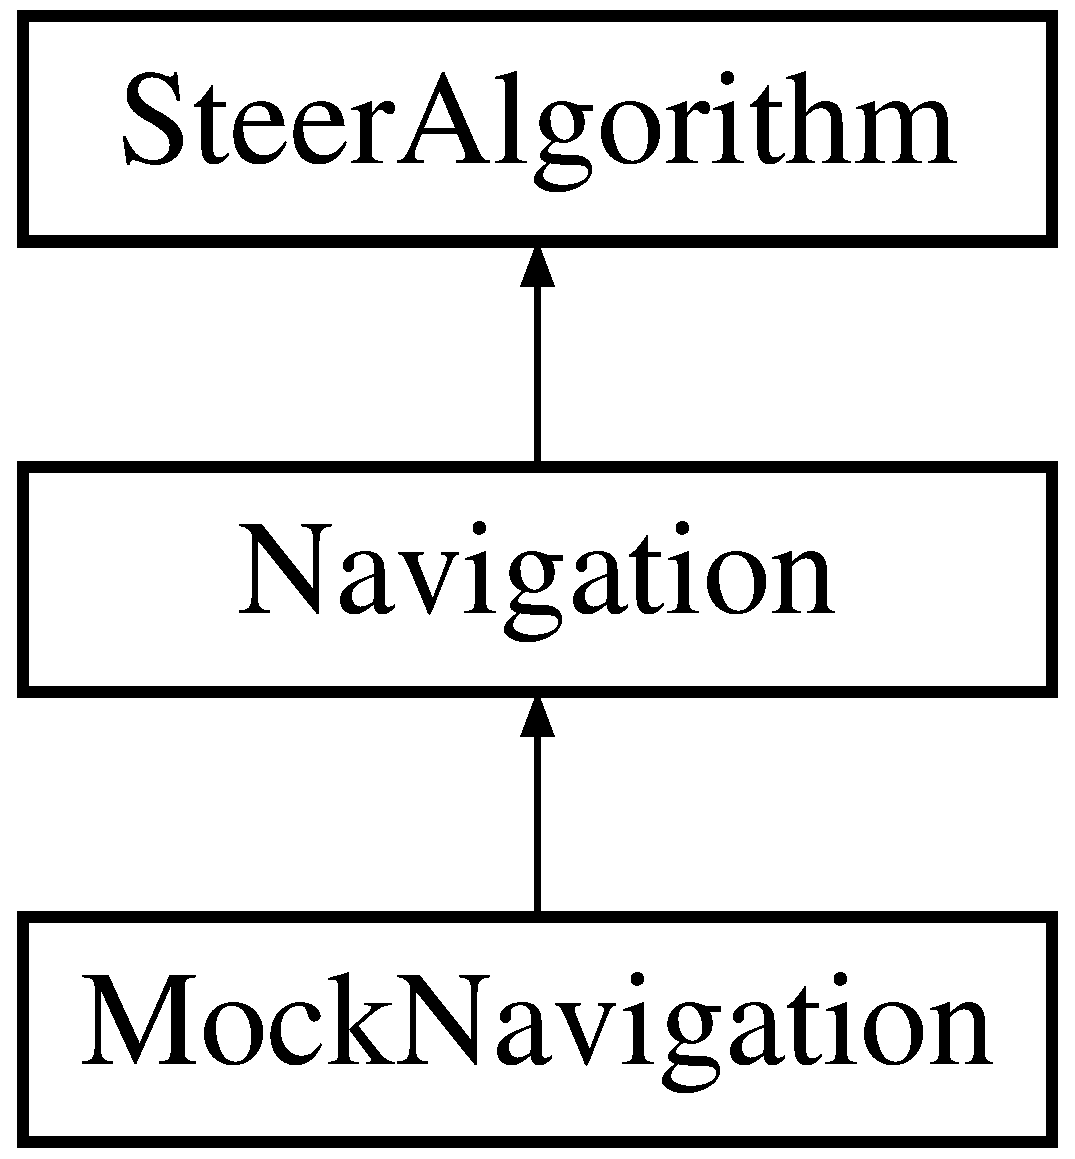
\includegraphics[height=3.000000cm]{class_mock_navigation}
\end{center}
\end{figure}
\subsection*{Public Member Functions}
\begin{DoxyCompactItemize}
\item 
\hyperlink{class_mock_navigation_a54759f67f52b03841f44efe7926fff22}{Mock\+Navigation} ()
\begin{DoxyCompactList}\small\item\em Initialise the constructor. \end{DoxyCompactList}\item 
\hyperlink{class_mock_navigation_acd53221a46f65f159ad53d22d3db1c51}{M\+O\+C\+K\+\_\+\+M\+E\+T\+H\+O\+D0} (\hyperlink{class_navigation_ab1469d74f4838a9d32a8647d22701f9f}{get\+Kp\+\_\+}, double())
\begin{DoxyCompactList}\small\item\em Mock method to get Kp\+\_\+. \end{DoxyCompactList}\item 
\hyperlink{class_mock_navigation_af40d1b1fb60d8bfe8a53ab5d91109b63}{M\+O\+C\+K\+\_\+\+M\+E\+T\+H\+O\+D1} (\hyperlink{class_navigation_a6dd95f46ff4ecc69895452a1879c30af}{set\+Kp\+\_\+}, bool(double))
\begin{DoxyCompactList}\small\item\em Mock method to set Kp\+\_\+. \end{DoxyCompactList}\item 
\hyperlink{class_mock_navigation_aa8fa53a73e8d9774d41fea23d7ecdb63}{M\+O\+C\+K\+\_\+\+M\+E\+T\+H\+O\+D0} (\hyperlink{class_navigation_a1a84392d6cce3f60df452ab482b5647c}{get\+Ki\+\_\+}, double())
\begin{DoxyCompactList}\small\item\em Mock method to get Ki\+\_\+. \end{DoxyCompactList}\item 
\hyperlink{class_mock_navigation_aa7670f64f701f2f174b991362ea11081}{M\+O\+C\+K\+\_\+\+M\+E\+T\+H\+O\+D1} (\hyperlink{class_navigation_a539d10206ceb162171e39c36e8aa8f0f}{set\+Ki\+\_\+}, bool(double))
\begin{DoxyCompactList}\small\item\em Mock method to set Ki\+\_\+. \end{DoxyCompactList}\item 
\hyperlink{class_mock_navigation_adc8e4d41452d78b00729b9327c635ea1}{M\+O\+C\+K\+\_\+\+M\+E\+T\+H\+O\+D0} (\hyperlink{class_navigation_ac6441bb601483166ef7a8081b76f634d}{get\+Kd\+\_\+}, double())
\begin{DoxyCompactList}\small\item\em Mock method to get Kd\+\_\+. \end{DoxyCompactList}\item 
\hyperlink{class_mock_navigation_acb06c66920ae8ff1f96ba4c9b079deaf}{M\+O\+C\+K\+\_\+\+M\+E\+T\+H\+O\+D1} (\hyperlink{class_navigation_a4986e4357d9707ddf92cf8f559ef3dce}{set\+Kd\+\_\+}, bool(double))
\begin{DoxyCompactList}\small\item\em Mock method to set Kd\+\_\+. \end{DoxyCompactList}\item 
\hyperlink{class_mock_navigation_a6289387acc5f11297d7a765241a499b4}{M\+O\+C\+K\+\_\+\+M\+E\+T\+H\+O\+D2} (\hyperlink{class_navigation_ae8fc8426c7277de0b34aec951fc28e2c}{calculate\+P\+ID}, std\+::vector$<$ double $>$(double, double))
\begin{DoxyCompactList}\small\item\em Mock method to calculate P\+ID. \end{DoxyCompactList}\item 
\hyperlink{class_mock_navigation_a5189068e3bbe0eeb377a119eaa8f0b62}{M\+O\+C\+K\+\_\+\+M\+E\+T\+H\+O\+D4} (\hyperlink{class_navigation_a0f83b511cec12a68f2c3466c40c5d3cb}{calculate}, double(double \hyperlink{class_steer_algorithm_a071efeb53e86ee949940b0ab10986044}{target\+Heading}, double current\+Velocity, double set\+Point, int flag))
\begin{DoxyCompactList}\small\item\em Mock method to compute the convergence. \end{DoxyCompactList}\end{DoxyCompactItemize}
\subsection*{Additional Inherited Members}


\subsection{Detailed Description}
Mock Class \hyperlink{class_navigation}{Navigation} To implement google mock. 

Definition at line 43 of file mock\+Navigation.\+cpp.



\subsection{Constructor \& Destructor Documentation}
\index{Mock\+Navigation@{Mock\+Navigation}!Mock\+Navigation@{Mock\+Navigation}}
\index{Mock\+Navigation@{Mock\+Navigation}!Mock\+Navigation@{Mock\+Navigation}}
\subsubsection[{\texorpdfstring{Mock\+Navigation()}{MockNavigation()}}]{\setlength{\rightskip}{0pt plus 5cm}Mock\+Navigation\+::\+Mock\+Navigation (
\begin{DoxyParamCaption}
{}
\end{DoxyParamCaption}
)\hspace{0.3cm}{\ttfamily [inline]}}\hypertarget{class_mock_navigation_a54759f67f52b03841f44efe7926fff22}{}\label{class_mock_navigation_a54759f67f52b03841f44efe7926fff22}


Initialise the constructor. 



Definition at line 48 of file mock\+Navigation.\+cpp.



\subsection{Member Function Documentation}
\index{Mock\+Navigation@{Mock\+Navigation}!M\+O\+C\+K\+\_\+\+M\+E\+T\+H\+O\+D0@{M\+O\+C\+K\+\_\+\+M\+E\+T\+H\+O\+D0}}
\index{M\+O\+C\+K\+\_\+\+M\+E\+T\+H\+O\+D0@{M\+O\+C\+K\+\_\+\+M\+E\+T\+H\+O\+D0}!Mock\+Navigation@{Mock\+Navigation}}
\subsubsection[{\texorpdfstring{M\+O\+C\+K\+\_\+\+M\+E\+T\+H\+O\+D0(get\+Kp\+\_\+, double())}{MOCK_METHOD0(getKp_, double())}}]{\setlength{\rightskip}{0pt plus 5cm}Mock\+Navigation\+::\+M\+O\+C\+K\+\_\+\+M\+E\+T\+H\+O\+D0 (
\begin{DoxyParamCaption}
\item[{{\bf get\+Kp\+\_\+}}]{, }
\item[{double()}]{}
\end{DoxyParamCaption}
)}\hypertarget{class_mock_navigation_acd53221a46f65f159ad53d22d3db1c51}{}\label{class_mock_navigation_acd53221a46f65f159ad53d22d3db1c51}


Mock method to get Kp\+\_\+. 

\index{Mock\+Navigation@{Mock\+Navigation}!M\+O\+C\+K\+\_\+\+M\+E\+T\+H\+O\+D0@{M\+O\+C\+K\+\_\+\+M\+E\+T\+H\+O\+D0}}
\index{M\+O\+C\+K\+\_\+\+M\+E\+T\+H\+O\+D0@{M\+O\+C\+K\+\_\+\+M\+E\+T\+H\+O\+D0}!Mock\+Navigation@{Mock\+Navigation}}
\subsubsection[{\texorpdfstring{M\+O\+C\+K\+\_\+\+M\+E\+T\+H\+O\+D0(get\+Ki\+\_\+, double())}{MOCK_METHOD0(getKi_, double())}}]{\setlength{\rightskip}{0pt plus 5cm}Mock\+Navigation\+::\+M\+O\+C\+K\+\_\+\+M\+E\+T\+H\+O\+D0 (
\begin{DoxyParamCaption}
\item[{{\bf get\+Ki\+\_\+}}]{, }
\item[{double()}]{}
\end{DoxyParamCaption}
)}\hypertarget{class_mock_navigation_aa8fa53a73e8d9774d41fea23d7ecdb63}{}\label{class_mock_navigation_aa8fa53a73e8d9774d41fea23d7ecdb63}


Mock method to get Ki\+\_\+. 

\index{Mock\+Navigation@{Mock\+Navigation}!M\+O\+C\+K\+\_\+\+M\+E\+T\+H\+O\+D0@{M\+O\+C\+K\+\_\+\+M\+E\+T\+H\+O\+D0}}
\index{M\+O\+C\+K\+\_\+\+M\+E\+T\+H\+O\+D0@{M\+O\+C\+K\+\_\+\+M\+E\+T\+H\+O\+D0}!Mock\+Navigation@{Mock\+Navigation}}
\subsubsection[{\texorpdfstring{M\+O\+C\+K\+\_\+\+M\+E\+T\+H\+O\+D0(get\+Kd\+\_\+, double())}{MOCK_METHOD0(getKd_, double())}}]{\setlength{\rightskip}{0pt plus 5cm}Mock\+Navigation\+::\+M\+O\+C\+K\+\_\+\+M\+E\+T\+H\+O\+D0 (
\begin{DoxyParamCaption}
\item[{{\bf get\+Kd\+\_\+}}]{, }
\item[{double()}]{}
\end{DoxyParamCaption}
)}\hypertarget{class_mock_navigation_adc8e4d41452d78b00729b9327c635ea1}{}\label{class_mock_navigation_adc8e4d41452d78b00729b9327c635ea1}


Mock method to get Kd\+\_\+. 

\index{Mock\+Navigation@{Mock\+Navigation}!M\+O\+C\+K\+\_\+\+M\+E\+T\+H\+O\+D1@{M\+O\+C\+K\+\_\+\+M\+E\+T\+H\+O\+D1}}
\index{M\+O\+C\+K\+\_\+\+M\+E\+T\+H\+O\+D1@{M\+O\+C\+K\+\_\+\+M\+E\+T\+H\+O\+D1}!Mock\+Navigation@{Mock\+Navigation}}
\subsubsection[{\texorpdfstring{M\+O\+C\+K\+\_\+\+M\+E\+T\+H\+O\+D1(set\+Kp\+\_\+, bool(double))}{MOCK_METHOD1(setKp_, bool(double))}}]{\setlength{\rightskip}{0pt plus 5cm}Mock\+Navigation\+::\+M\+O\+C\+K\+\_\+\+M\+E\+T\+H\+O\+D1 (
\begin{DoxyParamCaption}
\item[{{\bf set\+Kp\+\_\+}}]{, }
\item[{bool(double)}]{}
\end{DoxyParamCaption}
)}\hypertarget{class_mock_navigation_af40d1b1fb60d8bfe8a53ab5d91109b63}{}\label{class_mock_navigation_af40d1b1fb60d8bfe8a53ab5d91109b63}


Mock method to set Kp\+\_\+. 

\index{Mock\+Navigation@{Mock\+Navigation}!M\+O\+C\+K\+\_\+\+M\+E\+T\+H\+O\+D1@{M\+O\+C\+K\+\_\+\+M\+E\+T\+H\+O\+D1}}
\index{M\+O\+C\+K\+\_\+\+M\+E\+T\+H\+O\+D1@{M\+O\+C\+K\+\_\+\+M\+E\+T\+H\+O\+D1}!Mock\+Navigation@{Mock\+Navigation}}
\subsubsection[{\texorpdfstring{M\+O\+C\+K\+\_\+\+M\+E\+T\+H\+O\+D1(set\+Ki\+\_\+, bool(double))}{MOCK_METHOD1(setKi_, bool(double))}}]{\setlength{\rightskip}{0pt plus 5cm}Mock\+Navigation\+::\+M\+O\+C\+K\+\_\+\+M\+E\+T\+H\+O\+D1 (
\begin{DoxyParamCaption}
\item[{{\bf set\+Ki\+\_\+}}]{, }
\item[{bool(double)}]{}
\end{DoxyParamCaption}
)}\hypertarget{class_mock_navigation_aa7670f64f701f2f174b991362ea11081}{}\label{class_mock_navigation_aa7670f64f701f2f174b991362ea11081}


Mock method to set Ki\+\_\+. 

\index{Mock\+Navigation@{Mock\+Navigation}!M\+O\+C\+K\+\_\+\+M\+E\+T\+H\+O\+D1@{M\+O\+C\+K\+\_\+\+M\+E\+T\+H\+O\+D1}}
\index{M\+O\+C\+K\+\_\+\+M\+E\+T\+H\+O\+D1@{M\+O\+C\+K\+\_\+\+M\+E\+T\+H\+O\+D1}!Mock\+Navigation@{Mock\+Navigation}}
\subsubsection[{\texorpdfstring{M\+O\+C\+K\+\_\+\+M\+E\+T\+H\+O\+D1(set\+Kd\+\_\+, bool(double))}{MOCK_METHOD1(setKd_, bool(double))}}]{\setlength{\rightskip}{0pt plus 5cm}Mock\+Navigation\+::\+M\+O\+C\+K\+\_\+\+M\+E\+T\+H\+O\+D1 (
\begin{DoxyParamCaption}
\item[{{\bf set\+Kd\+\_\+}}]{, }
\item[{bool(double)}]{}
\end{DoxyParamCaption}
)}\hypertarget{class_mock_navigation_acb06c66920ae8ff1f96ba4c9b079deaf}{}\label{class_mock_navigation_acb06c66920ae8ff1f96ba4c9b079deaf}


Mock method to set Kd\+\_\+. 

\index{Mock\+Navigation@{Mock\+Navigation}!M\+O\+C\+K\+\_\+\+M\+E\+T\+H\+O\+D2@{M\+O\+C\+K\+\_\+\+M\+E\+T\+H\+O\+D2}}
\index{M\+O\+C\+K\+\_\+\+M\+E\+T\+H\+O\+D2@{M\+O\+C\+K\+\_\+\+M\+E\+T\+H\+O\+D2}!Mock\+Navigation@{Mock\+Navigation}}
\subsubsection[{\texorpdfstring{M\+O\+C\+K\+\_\+\+M\+E\+T\+H\+O\+D2(calculate\+P\+I\+D, std\+::vector$<$ double $>$(double, double))}{MOCK_METHOD2(calculatePID, std::vector< double >(double, double))}}]{\setlength{\rightskip}{0pt plus 5cm}Mock\+Navigation\+::\+M\+O\+C\+K\+\_\+\+M\+E\+T\+H\+O\+D2 (
\begin{DoxyParamCaption}
\item[{{\bf calculate\+P\+ID}}]{, }
\item[{std\+::vector$<$ double $>$}]{double, double}
\end{DoxyParamCaption}
)}\hypertarget{class_mock_navigation_a6289387acc5f11297d7a765241a499b4}{}\label{class_mock_navigation_a6289387acc5f11297d7a765241a499b4}


Mock method to calculate P\+ID. 

\index{Mock\+Navigation@{Mock\+Navigation}!M\+O\+C\+K\+\_\+\+M\+E\+T\+H\+O\+D4@{M\+O\+C\+K\+\_\+\+M\+E\+T\+H\+O\+D4}}
\index{M\+O\+C\+K\+\_\+\+M\+E\+T\+H\+O\+D4@{M\+O\+C\+K\+\_\+\+M\+E\+T\+H\+O\+D4}!Mock\+Navigation@{Mock\+Navigation}}
\subsubsection[{\texorpdfstring{M\+O\+C\+K\+\_\+\+M\+E\+T\+H\+O\+D4(calculate, double(double target\+Heading, double current\+Velocity, double set\+Point, int flag))}{MOCK_METHOD4(calculate, double(double targetHeading, double currentVelocity, double setPoint, int flag))}}]{\setlength{\rightskip}{0pt plus 5cm}Mock\+Navigation\+::\+M\+O\+C\+K\+\_\+\+M\+E\+T\+H\+O\+D4 (
\begin{DoxyParamCaption}
\item[{{\bf calculate}}]{, }
\item[{double(double {\bf target\+Heading}, double current\+Velocity, double set\+Point, int flag)}]{}
\end{DoxyParamCaption}
)}\hypertarget{class_mock_navigation_a5189068e3bbe0eeb377a119eaa8f0b62}{}\label{class_mock_navigation_a5189068e3bbe0eeb377a119eaa8f0b62}


Mock method to compute the convergence. 



The documentation for this class was generated from the following file\+:\begin{DoxyCompactItemize}
\item 
test/\hyperlink{mock_navigation_8cpp}{mock\+Navigation.\+cpp}\end{DoxyCompactItemize}

\hypertarget{structgnuplotio_1_1_mode1_d}{}\section{gnuplotio\+:\+:Mode1D Struct Reference}
\label{structgnuplotio_1_1_mode1_d}\index{gnuplotio\+::\+Mode1D@{gnuplotio\+::\+Mode1D}}


{\ttfamily \#include $<$gnuplot-\/iostream.\+h$>$}

\subsection*{Static Public Member Functions}
\begin{DoxyCompactItemize}
\item 
static std\+::string \hyperlink{structgnuplotio_1_1_mode1_d_a508d170d84da4dfb7cd07eebad894b8f}{class\+\_\+name} ()
\end{DoxyCompactItemize}


\subsection{Detailed Description}


Definition at line 1207 of file gnuplot-\/iostream.\+h.



\subsection{Member Function Documentation}
\index{gnuplotio\+::\+Mode1D@{gnuplotio\+::\+Mode1D}!class\+\_\+name@{class\+\_\+name}}
\index{class\+\_\+name@{class\+\_\+name}!gnuplotio\+::\+Mode1D@{gnuplotio\+::\+Mode1D}}
\subsubsection[{\texorpdfstring{class\+\_\+name()}{class_name()}}]{\setlength{\rightskip}{0pt plus 5cm}static std\+::string gnuplotio\+::\+Mode1\+D\+::class\+\_\+name (
\begin{DoxyParamCaption}
{}
\end{DoxyParamCaption}
)\hspace{0.3cm}{\ttfamily [inline]}, {\ttfamily [static]}}\hypertarget{structgnuplotio_1_1_mode1_d_a508d170d84da4dfb7cd07eebad894b8f}{}\label{structgnuplotio_1_1_mode1_d_a508d170d84da4dfb7cd07eebad894b8f}


Definition at line 1207 of file gnuplot-\/iostream.\+h.



The documentation for this struct was generated from the following file\+:\begin{DoxyCompactItemize}
\item 
include/\hyperlink{gnuplot-iostream_8h}{gnuplot-\/iostream.\+h}\end{DoxyCompactItemize}

\hypertarget{structgnuplotio_1_1_mode1_d_unwrap}{}\section{gnuplotio\+:\+:Mode1\+D\+Unwrap Struct Reference}
\label{structgnuplotio_1_1_mode1_d_unwrap}\index{gnuplotio\+::\+Mode1\+D\+Unwrap@{gnuplotio\+::\+Mode1\+D\+Unwrap}}


{\ttfamily \#include $<$gnuplot-\/iostream.\+h$>$}

\subsection*{Static Public Member Functions}
\begin{DoxyCompactItemize}
\item 
static std\+::string \hyperlink{structgnuplotio_1_1_mode1_d_unwrap_a2350096ad4d8b668f6df56c32cab69b6}{class\+\_\+name} ()
\end{DoxyCompactItemize}


\subsection{Detailed Description}


Definition at line 1209 of file gnuplot-\/iostream.\+h.



\subsection{Member Function Documentation}
\index{gnuplotio\+::\+Mode1\+D\+Unwrap@{gnuplotio\+::\+Mode1\+D\+Unwrap}!class\+\_\+name@{class\+\_\+name}}
\index{class\+\_\+name@{class\+\_\+name}!gnuplotio\+::\+Mode1\+D\+Unwrap@{gnuplotio\+::\+Mode1\+D\+Unwrap}}
\subsubsection[{\texorpdfstring{class\+\_\+name()}{class_name()}}]{\setlength{\rightskip}{0pt plus 5cm}static std\+::string gnuplotio\+::\+Mode1\+D\+Unwrap\+::class\+\_\+name (
\begin{DoxyParamCaption}
{}
\end{DoxyParamCaption}
)\hspace{0.3cm}{\ttfamily [inline]}, {\ttfamily [static]}}\hypertarget{structgnuplotio_1_1_mode1_d_unwrap_a2350096ad4d8b668f6df56c32cab69b6}{}\label{structgnuplotio_1_1_mode1_d_unwrap_a2350096ad4d8b668f6df56c32cab69b6}


Definition at line 1209 of file gnuplot-\/iostream.\+h.



The documentation for this struct was generated from the following file\+:\begin{DoxyCompactItemize}
\item 
include/\hyperlink{gnuplot-iostream_8h}{gnuplot-\/iostream.\+h}\end{DoxyCompactItemize}

\hypertarget{structgnuplotio_1_1_mode2_d}{}\section{gnuplotio\+:\+:Mode2D Struct Reference}
\label{structgnuplotio_1_1_mode2_d}\index{gnuplotio\+::\+Mode2D@{gnuplotio\+::\+Mode2D}}


{\ttfamily \#include $<$gnuplot-\/iostream.\+h$>$}

\subsection*{Static Public Member Functions}
\begin{DoxyCompactItemize}
\item 
static std\+::string \hyperlink{structgnuplotio_1_1_mode2_d_aaf35c9cd117de8bc5dbc2d5ec1224232}{class\+\_\+name} ()
\end{DoxyCompactItemize}


\subsection{Detailed Description}


Definition at line 1208 of file gnuplot-\/iostream.\+h.



\subsection{Member Function Documentation}
\index{gnuplotio\+::\+Mode2D@{gnuplotio\+::\+Mode2D}!class\+\_\+name@{class\+\_\+name}}
\index{class\+\_\+name@{class\+\_\+name}!gnuplotio\+::\+Mode2D@{gnuplotio\+::\+Mode2D}}
\subsubsection[{\texorpdfstring{class\+\_\+name()}{class_name()}}]{\setlength{\rightskip}{0pt plus 5cm}static std\+::string gnuplotio\+::\+Mode2\+D\+::class\+\_\+name (
\begin{DoxyParamCaption}
{}
\end{DoxyParamCaption}
)\hspace{0.3cm}{\ttfamily [inline]}, {\ttfamily [static]}}\hypertarget{structgnuplotio_1_1_mode2_d_aaf35c9cd117de8bc5dbc2d5ec1224232}{}\label{structgnuplotio_1_1_mode2_d_aaf35c9cd117de8bc5dbc2d5ec1224232}


Definition at line 1208 of file gnuplot-\/iostream.\+h.



The documentation for this struct was generated from the following file\+:\begin{DoxyCompactItemize}
\item 
include/\hyperlink{gnuplot-iostream_8h}{gnuplot-\/iostream.\+h}\end{DoxyCompactItemize}

\hypertarget{structgnuplotio_1_1_mode2_d_unwrap}{}\section{gnuplotio\+:\+:Mode2\+D\+Unwrap Struct Reference}
\label{structgnuplotio_1_1_mode2_d_unwrap}\index{gnuplotio\+::\+Mode2\+D\+Unwrap@{gnuplotio\+::\+Mode2\+D\+Unwrap}}


{\ttfamily \#include $<$gnuplot-\/iostream.\+h$>$}

\subsection*{Static Public Member Functions}
\begin{DoxyCompactItemize}
\item 
static std\+::string \hyperlink{structgnuplotio_1_1_mode2_d_unwrap_ab2f533c9ceb52cfecaa161c64316deb9}{class\+\_\+name} ()
\end{DoxyCompactItemize}


\subsection{Detailed Description}


Definition at line 1210 of file gnuplot-\/iostream.\+h.



\subsection{Member Function Documentation}
\index{gnuplotio\+::\+Mode2\+D\+Unwrap@{gnuplotio\+::\+Mode2\+D\+Unwrap}!class\+\_\+name@{class\+\_\+name}}
\index{class\+\_\+name@{class\+\_\+name}!gnuplotio\+::\+Mode2\+D\+Unwrap@{gnuplotio\+::\+Mode2\+D\+Unwrap}}
\subsubsection[{\texorpdfstring{class\+\_\+name()}{class_name()}}]{\setlength{\rightskip}{0pt plus 5cm}static std\+::string gnuplotio\+::\+Mode2\+D\+Unwrap\+::class\+\_\+name (
\begin{DoxyParamCaption}
{}
\end{DoxyParamCaption}
)\hspace{0.3cm}{\ttfamily [inline]}, {\ttfamily [static]}}\hypertarget{structgnuplotio_1_1_mode2_d_unwrap_ab2f533c9ceb52cfecaa161c64316deb9}{}\label{structgnuplotio_1_1_mode2_d_unwrap_ab2f533c9ceb52cfecaa161c64316deb9}


Definition at line 1210 of file gnuplot-\/iostream.\+h.



The documentation for this struct was generated from the following file\+:\begin{DoxyCompactItemize}
\item 
include/\hyperlink{gnuplot-iostream_8h}{gnuplot-\/iostream.\+h}\end{DoxyCompactItemize}

\hypertarget{structgnuplotio_1_1_mode_auto}{}\section{gnuplotio\+:\+:Mode\+Auto Struct Reference}
\label{structgnuplotio_1_1_mode_auto}\index{gnuplotio\+::\+Mode\+Auto@{gnuplotio\+::\+Mode\+Auto}}


{\ttfamily \#include $<$gnuplot-\/iostream.\+h$>$}

\subsection*{Static Public Member Functions}
\begin{DoxyCompactItemize}
\item 
static std\+::string \hyperlink{structgnuplotio_1_1_mode_auto_ac73f89a782ac32dd8bc7b8f7a7581523}{class\+\_\+name} ()
\end{DoxyCompactItemize}


\subsection{Detailed Description}


Definition at line 1212 of file gnuplot-\/iostream.\+h.



\subsection{Member Function Documentation}
\index{gnuplotio\+::\+Mode\+Auto@{gnuplotio\+::\+Mode\+Auto}!class\+\_\+name@{class\+\_\+name}}
\index{class\+\_\+name@{class\+\_\+name}!gnuplotio\+::\+Mode\+Auto@{gnuplotio\+::\+Mode\+Auto}}
\subsubsection[{\texorpdfstring{class\+\_\+name()}{class_name()}}]{\setlength{\rightskip}{0pt plus 5cm}static std\+::string gnuplotio\+::\+Mode\+Auto\+::class\+\_\+name (
\begin{DoxyParamCaption}
{}
\end{DoxyParamCaption}
)\hspace{0.3cm}{\ttfamily [inline]}, {\ttfamily [static]}}\hypertarget{structgnuplotio_1_1_mode_auto_ac73f89a782ac32dd8bc7b8f7a7581523}{}\label{structgnuplotio_1_1_mode_auto_ac73f89a782ac32dd8bc7b8f7a7581523}


Definition at line 1212 of file gnuplot-\/iostream.\+h.



The documentation for this struct was generated from the following file\+:\begin{DoxyCompactItemize}
\item 
include/\hyperlink{gnuplot-iostream_8h}{gnuplot-\/iostream.\+h}\end{DoxyCompactItemize}

\hypertarget{structgnuplotio_1_1_mode_auto_decoder}{}\section{gnuplotio\+:\+:Mode\+Auto\+Decoder$<$ T, Enable $>$ Struct Template Reference}
\label{structgnuplotio_1_1_mode_auto_decoder}\index{gnuplotio\+::\+Mode\+Auto\+Decoder$<$ T, Enable $>$@{gnuplotio\+::\+Mode\+Auto\+Decoder$<$ T, Enable $>$}}


{\ttfamily \#include $<$gnuplot-\/iostream.\+h$>$}



\subsection{Detailed Description}
\subsubsection*{template$<$typename T, typename Enable = void$>$\\*
struct gnuplotio\+::\+Mode\+Auto\+Decoder$<$ T, Enable $>$}



Definition at line 1224 of file gnuplot-\/iostream.\+h.



The documentation for this struct was generated from the following file\+:\begin{DoxyCompactItemize}
\item 
include/\hyperlink{gnuplot-iostream_8h}{gnuplot-\/iostream.\+h}\end{DoxyCompactItemize}

\hypertarget{structgnuplotio_1_1_mode_binary}{}\section{gnuplotio\+:\+:Mode\+Binary Struct Reference}
\label{structgnuplotio_1_1_mode_binary}\index{gnuplotio\+::\+Mode\+Binary@{gnuplotio\+::\+Mode\+Binary}}


{\ttfamily \#include $<$gnuplot-\/iostream.\+h$>$}

\subsection*{Static Public Attributes}
\begin{DoxyCompactItemize}
\item 
static const bool \hyperlink{structgnuplotio_1_1_mode_binary_ac89064b5df24f7ef4d765fdfde4fd1b6}{is\+\_\+text} = 0
\item 
static const bool \hyperlink{structgnuplotio_1_1_mode_binary_aee724034dc3372b8e12b1187507bf136}{is\+\_\+binfmt} = 0
\item 
static const bool \hyperlink{structgnuplotio_1_1_mode_binary_a6eae25ea662362bbb88bc987d6025290}{is\+\_\+size} = 0
\end{DoxyCompactItemize}


\subsection{Detailed Description}


Definition at line 1196 of file gnuplot-\/iostream.\+h.



\subsection{Member Data Documentation}
\index{gnuplotio\+::\+Mode\+Binary@{gnuplotio\+::\+Mode\+Binary}!is\+\_\+binfmt@{is\+\_\+binfmt}}
\index{is\+\_\+binfmt@{is\+\_\+binfmt}!gnuplotio\+::\+Mode\+Binary@{gnuplotio\+::\+Mode\+Binary}}
\subsubsection[{\texorpdfstring{is\+\_\+binfmt}{is_binfmt}}]{\setlength{\rightskip}{0pt plus 5cm}const bool gnuplotio\+::\+Mode\+Binary\+::is\+\_\+binfmt = 0\hspace{0.3cm}{\ttfamily [static]}}\hypertarget{structgnuplotio_1_1_mode_binary_aee724034dc3372b8e12b1187507bf136}{}\label{structgnuplotio_1_1_mode_binary_aee724034dc3372b8e12b1187507bf136}


Definition at line 1196 of file gnuplot-\/iostream.\+h.

\index{gnuplotio\+::\+Mode\+Binary@{gnuplotio\+::\+Mode\+Binary}!is\+\_\+size@{is\+\_\+size}}
\index{is\+\_\+size@{is\+\_\+size}!gnuplotio\+::\+Mode\+Binary@{gnuplotio\+::\+Mode\+Binary}}
\subsubsection[{\texorpdfstring{is\+\_\+size}{is_size}}]{\setlength{\rightskip}{0pt plus 5cm}const bool gnuplotio\+::\+Mode\+Binary\+::is\+\_\+size = 0\hspace{0.3cm}{\ttfamily [static]}}\hypertarget{structgnuplotio_1_1_mode_binary_a6eae25ea662362bbb88bc987d6025290}{}\label{structgnuplotio_1_1_mode_binary_a6eae25ea662362bbb88bc987d6025290}


Definition at line 1196 of file gnuplot-\/iostream.\+h.

\index{gnuplotio\+::\+Mode\+Binary@{gnuplotio\+::\+Mode\+Binary}!is\+\_\+text@{is\+\_\+text}}
\index{is\+\_\+text@{is\+\_\+text}!gnuplotio\+::\+Mode\+Binary@{gnuplotio\+::\+Mode\+Binary}}
\subsubsection[{\texorpdfstring{is\+\_\+text}{is_text}}]{\setlength{\rightskip}{0pt plus 5cm}const bool gnuplotio\+::\+Mode\+Binary\+::is\+\_\+text = 0\hspace{0.3cm}{\ttfamily [static]}}\hypertarget{structgnuplotio_1_1_mode_binary_ac89064b5df24f7ef4d765fdfde4fd1b6}{}\label{structgnuplotio_1_1_mode_binary_ac89064b5df24f7ef4d765fdfde4fd1b6}


Definition at line 1196 of file gnuplot-\/iostream.\+h.



The documentation for this struct was generated from the following file\+:\begin{DoxyCompactItemize}
\item 
include/\hyperlink{gnuplot-iostream_8h}{gnuplot-\/iostream.\+h}\end{DoxyCompactItemize}

\hypertarget{structgnuplotio_1_1_mode_binfmt}{}\section{gnuplotio\+:\+:Mode\+Binfmt Struct Reference}
\label{structgnuplotio_1_1_mode_binfmt}\index{gnuplotio\+::\+Mode\+Binfmt@{gnuplotio\+::\+Mode\+Binfmt}}


{\ttfamily \#include $<$gnuplot-\/iostream.\+h$>$}

\subsection*{Static Public Attributes}
\begin{DoxyCompactItemize}
\item 
static const bool \hyperlink{structgnuplotio_1_1_mode_binfmt_a7ab187fe922cac23b0d39ade81e5eb56}{is\+\_\+text} = 0
\item 
static const bool \hyperlink{structgnuplotio_1_1_mode_binfmt_ab0d5d3718364cdea0347f93ec121d841}{is\+\_\+binfmt} = 1
\item 
static const bool \hyperlink{structgnuplotio_1_1_mode_binfmt_a40a5a8ee815d6a5e9a3c30c8290a6967}{is\+\_\+size} = 0
\end{DoxyCompactItemize}


\subsection{Detailed Description}


Definition at line 1197 of file gnuplot-\/iostream.\+h.



\subsection{Member Data Documentation}
\index{gnuplotio\+::\+Mode\+Binfmt@{gnuplotio\+::\+Mode\+Binfmt}!is\+\_\+binfmt@{is\+\_\+binfmt}}
\index{is\+\_\+binfmt@{is\+\_\+binfmt}!gnuplotio\+::\+Mode\+Binfmt@{gnuplotio\+::\+Mode\+Binfmt}}
\subsubsection[{\texorpdfstring{is\+\_\+binfmt}{is_binfmt}}]{\setlength{\rightskip}{0pt plus 5cm}const bool gnuplotio\+::\+Mode\+Binfmt\+::is\+\_\+binfmt = 1\hspace{0.3cm}{\ttfamily [static]}}\hypertarget{structgnuplotio_1_1_mode_binfmt_ab0d5d3718364cdea0347f93ec121d841}{}\label{structgnuplotio_1_1_mode_binfmt_ab0d5d3718364cdea0347f93ec121d841}


Definition at line 1197 of file gnuplot-\/iostream.\+h.

\index{gnuplotio\+::\+Mode\+Binfmt@{gnuplotio\+::\+Mode\+Binfmt}!is\+\_\+size@{is\+\_\+size}}
\index{is\+\_\+size@{is\+\_\+size}!gnuplotio\+::\+Mode\+Binfmt@{gnuplotio\+::\+Mode\+Binfmt}}
\subsubsection[{\texorpdfstring{is\+\_\+size}{is_size}}]{\setlength{\rightskip}{0pt plus 5cm}const bool gnuplotio\+::\+Mode\+Binfmt\+::is\+\_\+size = 0\hspace{0.3cm}{\ttfamily [static]}}\hypertarget{structgnuplotio_1_1_mode_binfmt_a40a5a8ee815d6a5e9a3c30c8290a6967}{}\label{structgnuplotio_1_1_mode_binfmt_a40a5a8ee815d6a5e9a3c30c8290a6967}


Definition at line 1197 of file gnuplot-\/iostream.\+h.

\index{gnuplotio\+::\+Mode\+Binfmt@{gnuplotio\+::\+Mode\+Binfmt}!is\+\_\+text@{is\+\_\+text}}
\index{is\+\_\+text@{is\+\_\+text}!gnuplotio\+::\+Mode\+Binfmt@{gnuplotio\+::\+Mode\+Binfmt}}
\subsubsection[{\texorpdfstring{is\+\_\+text}{is_text}}]{\setlength{\rightskip}{0pt plus 5cm}const bool gnuplotio\+::\+Mode\+Binfmt\+::is\+\_\+text = 0\hspace{0.3cm}{\ttfamily [static]}}\hypertarget{structgnuplotio_1_1_mode_binfmt_a7ab187fe922cac23b0d39ade81e5eb56}{}\label{structgnuplotio_1_1_mode_binfmt_a7ab187fe922cac23b0d39ade81e5eb56}


Definition at line 1197 of file gnuplot-\/iostream.\+h.



The documentation for this struct was generated from the following file\+:\begin{DoxyCompactItemize}
\item 
include/\hyperlink{gnuplot-iostream_8h}{gnuplot-\/iostream.\+h}\end{DoxyCompactItemize}

\hypertarget{structgnuplotio_1_1_mode_size}{}\section{gnuplotio\+:\+:Mode\+Size Struct Reference}
\label{structgnuplotio_1_1_mode_size}\index{gnuplotio\+::\+Mode\+Size@{gnuplotio\+::\+Mode\+Size}}


{\ttfamily \#include $<$gnuplot-\/iostream.\+h$>$}

\subsection*{Static Public Attributes}
\begin{DoxyCompactItemize}
\item 
static const bool \hyperlink{structgnuplotio_1_1_mode_size_aa01840f76877ae7c8bad254dae28e32c}{is\+\_\+text} = 0
\item 
static const bool \hyperlink{structgnuplotio_1_1_mode_size_ac5243e8e4910f2f6a2724b9fc0de4ff9}{is\+\_\+binfmt} = 0
\item 
static const bool \hyperlink{structgnuplotio_1_1_mode_size_aa20ae9f1ce222504489db33d13eb46c0}{is\+\_\+size} = 1
\end{DoxyCompactItemize}


\subsection{Detailed Description}


Definition at line 1198 of file gnuplot-\/iostream.\+h.



\subsection{Member Data Documentation}
\index{gnuplotio\+::\+Mode\+Size@{gnuplotio\+::\+Mode\+Size}!is\+\_\+binfmt@{is\+\_\+binfmt}}
\index{is\+\_\+binfmt@{is\+\_\+binfmt}!gnuplotio\+::\+Mode\+Size@{gnuplotio\+::\+Mode\+Size}}
\subsubsection[{\texorpdfstring{is\+\_\+binfmt}{is_binfmt}}]{\setlength{\rightskip}{0pt plus 5cm}const bool gnuplotio\+::\+Mode\+Size\+::is\+\_\+binfmt = 0\hspace{0.3cm}{\ttfamily [static]}}\hypertarget{structgnuplotio_1_1_mode_size_ac5243e8e4910f2f6a2724b9fc0de4ff9}{}\label{structgnuplotio_1_1_mode_size_ac5243e8e4910f2f6a2724b9fc0de4ff9}


Definition at line 1198 of file gnuplot-\/iostream.\+h.

\index{gnuplotio\+::\+Mode\+Size@{gnuplotio\+::\+Mode\+Size}!is\+\_\+size@{is\+\_\+size}}
\index{is\+\_\+size@{is\+\_\+size}!gnuplotio\+::\+Mode\+Size@{gnuplotio\+::\+Mode\+Size}}
\subsubsection[{\texorpdfstring{is\+\_\+size}{is_size}}]{\setlength{\rightskip}{0pt plus 5cm}const bool gnuplotio\+::\+Mode\+Size\+::is\+\_\+size = 1\hspace{0.3cm}{\ttfamily [static]}}\hypertarget{structgnuplotio_1_1_mode_size_aa20ae9f1ce222504489db33d13eb46c0}{}\label{structgnuplotio_1_1_mode_size_aa20ae9f1ce222504489db33d13eb46c0}


Definition at line 1198 of file gnuplot-\/iostream.\+h.

\index{gnuplotio\+::\+Mode\+Size@{gnuplotio\+::\+Mode\+Size}!is\+\_\+text@{is\+\_\+text}}
\index{is\+\_\+text@{is\+\_\+text}!gnuplotio\+::\+Mode\+Size@{gnuplotio\+::\+Mode\+Size}}
\subsubsection[{\texorpdfstring{is\+\_\+text}{is_text}}]{\setlength{\rightskip}{0pt plus 5cm}const bool gnuplotio\+::\+Mode\+Size\+::is\+\_\+text = 0\hspace{0.3cm}{\ttfamily [static]}}\hypertarget{structgnuplotio_1_1_mode_size_aa01840f76877ae7c8bad254dae28e32c}{}\label{structgnuplotio_1_1_mode_size_aa01840f76877ae7c8bad254dae28e32c}


Definition at line 1198 of file gnuplot-\/iostream.\+h.



The documentation for this struct was generated from the following file\+:\begin{DoxyCompactItemize}
\item 
include/\hyperlink{gnuplot-iostream_8h}{gnuplot-\/iostream.\+h}\end{DoxyCompactItemize}

\hypertarget{structgnuplotio_1_1_mode_text}{}\section{gnuplotio\+:\+:Mode\+Text Struct Reference}
\label{structgnuplotio_1_1_mode_text}\index{gnuplotio\+::\+Mode\+Text@{gnuplotio\+::\+Mode\+Text}}


{\ttfamily \#include $<$gnuplot-\/iostream.\+h$>$}

\subsection*{Static Public Attributes}
\begin{DoxyCompactItemize}
\item 
static const bool \hyperlink{structgnuplotio_1_1_mode_text_a7083d8977c354a036a7c542bf99d3d52}{is\+\_\+text} = 1
\item 
static const bool \hyperlink{structgnuplotio_1_1_mode_text_a4c771363d894ae64d6af961ffde35126}{is\+\_\+binfmt} = 0
\item 
static const bool \hyperlink{structgnuplotio_1_1_mode_text_aaffc1e7bb26c6d1404cb5a3f03f13be9}{is\+\_\+size} = 0
\end{DoxyCompactItemize}


\subsection{Detailed Description}


Definition at line 1195 of file gnuplot-\/iostream.\+h.



\subsection{Member Data Documentation}
\index{gnuplotio\+::\+Mode\+Text@{gnuplotio\+::\+Mode\+Text}!is\+\_\+binfmt@{is\+\_\+binfmt}}
\index{is\+\_\+binfmt@{is\+\_\+binfmt}!gnuplotio\+::\+Mode\+Text@{gnuplotio\+::\+Mode\+Text}}
\subsubsection[{\texorpdfstring{is\+\_\+binfmt}{is_binfmt}}]{\setlength{\rightskip}{0pt plus 5cm}const bool gnuplotio\+::\+Mode\+Text\+::is\+\_\+binfmt = 0\hspace{0.3cm}{\ttfamily [static]}}\hypertarget{structgnuplotio_1_1_mode_text_a4c771363d894ae64d6af961ffde35126}{}\label{structgnuplotio_1_1_mode_text_a4c771363d894ae64d6af961ffde35126}


Definition at line 1195 of file gnuplot-\/iostream.\+h.

\index{gnuplotio\+::\+Mode\+Text@{gnuplotio\+::\+Mode\+Text}!is\+\_\+size@{is\+\_\+size}}
\index{is\+\_\+size@{is\+\_\+size}!gnuplotio\+::\+Mode\+Text@{gnuplotio\+::\+Mode\+Text}}
\subsubsection[{\texorpdfstring{is\+\_\+size}{is_size}}]{\setlength{\rightskip}{0pt plus 5cm}const bool gnuplotio\+::\+Mode\+Text\+::is\+\_\+size = 0\hspace{0.3cm}{\ttfamily [static]}}\hypertarget{structgnuplotio_1_1_mode_text_aaffc1e7bb26c6d1404cb5a3f03f13be9}{}\label{structgnuplotio_1_1_mode_text_aaffc1e7bb26c6d1404cb5a3f03f13be9}


Definition at line 1195 of file gnuplot-\/iostream.\+h.

\index{gnuplotio\+::\+Mode\+Text@{gnuplotio\+::\+Mode\+Text}!is\+\_\+text@{is\+\_\+text}}
\index{is\+\_\+text@{is\+\_\+text}!gnuplotio\+::\+Mode\+Text@{gnuplotio\+::\+Mode\+Text}}
\subsubsection[{\texorpdfstring{is\+\_\+text}{is_text}}]{\setlength{\rightskip}{0pt plus 5cm}const bool gnuplotio\+::\+Mode\+Text\+::is\+\_\+text = 1\hspace{0.3cm}{\ttfamily [static]}}\hypertarget{structgnuplotio_1_1_mode_text_a7083d8977c354a036a7c542bf99d3d52}{}\label{structgnuplotio_1_1_mode_text_a7083d8977c354a036a7c542bf99d3d52}


Definition at line 1195 of file gnuplot-\/iostream.\+h.



The documentation for this struct was generated from the following file\+:\begin{DoxyCompactItemize}
\item 
include/\hyperlink{gnuplot-iostream_8h}{gnuplot-\/iostream.\+h}\end{DoxyCompactItemize}

\hypertarget{class_navigation}{}\section{Navigation Class Reference}
\label{class_navigation}\index{Navigation@{Navigation}}


Class \hyperlink{class_navigation}{Navigation} Contains the methods of Pid Algorithm.  




{\ttfamily \#include $<$Navigation.\+hpp$>$}



Inheritance diagram for Navigation\+:
\nopagebreak
\begin{figure}[H]
\begin{center}
\leavevmode
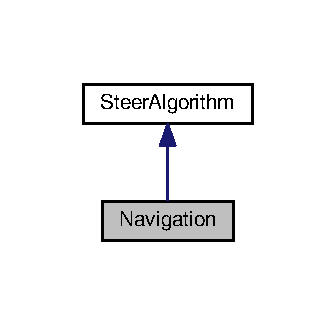
\includegraphics[width=161pt]{class_navigation__inherit__graph}
\end{center}
\end{figure}


Collaboration diagram for Navigation\+:
\nopagebreak
\begin{figure}[H]
\begin{center}
\leavevmode
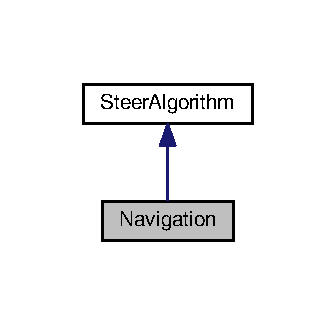
\includegraphics[width=161pt]{class_navigation__coll__graph}
\end{center}
\end{figure}
\subsection*{Public Member Functions}
\begin{DoxyCompactItemize}
\item 
\hyperlink{class_navigation_a81fdffdefe46340da5fa6c570066b42b}{Navigation} ()\hypertarget{class_navigation_a81fdffdefe46340da5fa6c570066b42b}{}\label{class_navigation_a81fdffdefe46340da5fa6c570066b42b}

\begin{DoxyCompactList}\small\item\em Constructor of class \hyperlink{class_navigation}{Navigation}. \end{DoxyCompactList}\item 
\hyperlink{class_navigation_addd4022d716df48f4e55a1db69361ba7}{$\sim$\+Navigation} ()\hypertarget{class_navigation_addd4022d716df48f4e55a1db69361ba7}{}\label{class_navigation_addd4022d716df48f4e55a1db69361ba7}

\begin{DoxyCompactList}\small\item\em Destructor of class \hyperlink{class_navigation}{Navigation}. \end{DoxyCompactList}\item 
double \hyperlink{class_navigation_a0eb1833ccc91d6fd5822938797686708}{calculate} (double current\+Velocity, double set\+Point, int flag)
\begin{DoxyCompactList}\small\item\em Function to calculate new velocity with a P\+ID Algorithm using kp, ki \& kd. \end{DoxyCompactList}\item 
double \hyperlink{class_navigation_ab1469d74f4838a9d32a8647d22701f9f}{get\+Kp\+\_\+} ()
\begin{DoxyCompactList}\small\item\em Function to get kp\+\_\+. \end{DoxyCompactList}\item 
double \hyperlink{class_navigation_a1a84392d6cce3f60df452ab482b5647c}{get\+Ki\+\_\+} ()
\begin{DoxyCompactList}\small\item\em Function to get ki\+\_\+. \end{DoxyCompactList}\item 
double \hyperlink{class_navigation_ac6441bb601483166ef7a8081b76f634d}{get\+Kd\+\_\+} ()
\begin{DoxyCompactList}\small\item\em Function to get kd\+\_\+. \end{DoxyCompactList}\item 
bool \hyperlink{class_navigation_a6dd95f46ff4ecc69895452a1879c30af}{set\+Kp\+\_\+} (double kp)
\begin{DoxyCompactList}\small\item\em Function to set kp\+\_\+. \end{DoxyCompactList}\item 
bool \hyperlink{class_navigation_a539d10206ceb162171e39c36e8aa8f0f}{set\+Ki\+\_\+} (double ki)
\begin{DoxyCompactList}\small\item\em Function to set ki\+\_\+. \end{DoxyCompactList}\item 
bool \hyperlink{class_navigation_a4986e4357d9707ddf92cf8f559ef3dce}{set\+Kd\+\_\+} (double kd)
\begin{DoxyCompactList}\small\item\em Function to set kd\+\_\+. \end{DoxyCompactList}\end{DoxyCompactItemize}
\subsection*{Public Attributes}
\begin{DoxyCompactItemize}
\item 
bool {\bfseries motor\+Direction} = true\hypertarget{class_navigation_ad7d7a5d5d1abe99e6b0f31ddb4794252}{}\label{class_navigation_ad7d7a5d5d1abe99e6b0f31ddb4794252}

\end{DoxyCompactItemize}


\subsection{Detailed Description}
Class \hyperlink{class_navigation}{Navigation} Contains the methods of Pid Algorithm. 

\subsection{Member Function Documentation}
\index{Navigation@{Navigation}!calculate@{calculate}}
\index{calculate@{calculate}!Navigation@{Navigation}}
\subsubsection[{\texorpdfstring{calculate(double current\+Velocity, double set\+Point, int flag)}{calculate(double currentVelocity, double setPoint, int flag)}}]{\setlength{\rightskip}{0pt plus 5cm}double Navigation\+::calculate (
\begin{DoxyParamCaption}
\item[{double}]{current\+Velocity, }
\item[{double}]{set\+Point, }
\item[{int}]{flag}
\end{DoxyParamCaption}
)}\hypertarget{class_navigation_a0eb1833ccc91d6fd5822938797686708}{}\label{class_navigation_a0eb1833ccc91d6fd5822938797686708}


Function to calculate new velocity with a P\+ID Algorithm using kp, ki \& kd. 


\begin{DoxyParams}{Parameters}
{\em double} & current\+Velocity, current velocity of robot \\
\hline
{\em double} & set\+Point, Target Velocity \\
\hline
{\em int} & flag, to enable while \\
\hline
\end{DoxyParams}
\begin{DoxyReturn}{Returns}
double ne\+Velocity 
\end{DoxyReturn}
\index{Navigation@{Navigation}!get\+Kd\+\_\+@{get\+Kd\+\_\+}}
\index{get\+Kd\+\_\+@{get\+Kd\+\_\+}!Navigation@{Navigation}}
\subsubsection[{\texorpdfstring{get\+Kd\+\_\+()}{getKd_()}}]{\setlength{\rightskip}{0pt plus 5cm}double Navigation\+::get\+Kd\+\_\+ (
\begin{DoxyParamCaption}
{}
\end{DoxyParamCaption}
)}\hypertarget{class_navigation_ac6441bb601483166ef7a8081b76f634d}{}\label{class_navigation_ac6441bb601483166ef7a8081b76f634d}


Function to get kd\+\_\+. 


\begin{DoxyParams}{Parameters}
{\em none} & \\
\hline
\end{DoxyParams}
\begin{DoxyReturn}{Returns}
double 
\end{DoxyReturn}
\index{Navigation@{Navigation}!get\+Ki\+\_\+@{get\+Ki\+\_\+}}
\index{get\+Ki\+\_\+@{get\+Ki\+\_\+}!Navigation@{Navigation}}
\subsubsection[{\texorpdfstring{get\+Ki\+\_\+()}{getKi_()}}]{\setlength{\rightskip}{0pt plus 5cm}double Navigation\+::get\+Ki\+\_\+ (
\begin{DoxyParamCaption}
{}
\end{DoxyParamCaption}
)}\hypertarget{class_navigation_a1a84392d6cce3f60df452ab482b5647c}{}\label{class_navigation_a1a84392d6cce3f60df452ab482b5647c}


Function to get ki\+\_\+. 


\begin{DoxyParams}{Parameters}
{\em none} & \\
\hline
\end{DoxyParams}
\begin{DoxyReturn}{Returns}
double 
\end{DoxyReturn}
\index{Navigation@{Navigation}!get\+Kp\+\_\+@{get\+Kp\+\_\+}}
\index{get\+Kp\+\_\+@{get\+Kp\+\_\+}!Navigation@{Navigation}}
\subsubsection[{\texorpdfstring{get\+Kp\+\_\+()}{getKp_()}}]{\setlength{\rightskip}{0pt plus 5cm}double Navigation\+::get\+Kp\+\_\+ (
\begin{DoxyParamCaption}
{}
\end{DoxyParamCaption}
)}\hypertarget{class_navigation_ab1469d74f4838a9d32a8647d22701f9f}{}\label{class_navigation_ab1469d74f4838a9d32a8647d22701f9f}


Function to get kp\+\_\+. 


\begin{DoxyParams}{Parameters}
{\em none} & \\
\hline
\end{DoxyParams}
\begin{DoxyReturn}{Returns}
double 
\end{DoxyReturn}
\index{Navigation@{Navigation}!set\+Kd\+\_\+@{set\+Kd\+\_\+}}
\index{set\+Kd\+\_\+@{set\+Kd\+\_\+}!Navigation@{Navigation}}
\subsubsection[{\texorpdfstring{set\+Kd\+\_\+(double kd)}{setKd_(double kd)}}]{\setlength{\rightskip}{0pt plus 5cm}bool Navigation\+::set\+Kd\+\_\+ (
\begin{DoxyParamCaption}
\item[{double}]{kd}
\end{DoxyParamCaption}
)}\hypertarget{class_navigation_a4986e4357d9707ddf92cf8f559ef3dce}{}\label{class_navigation_a4986e4357d9707ddf92cf8f559ef3dce}


Function to set kd\+\_\+. 


\begin{DoxyParams}{Parameters}
{\em double} & kd \\
\hline
\end{DoxyParams}
\begin{DoxyReturn}{Returns}
boolean true 
\end{DoxyReturn}
\index{Navigation@{Navigation}!set\+Ki\+\_\+@{set\+Ki\+\_\+}}
\index{set\+Ki\+\_\+@{set\+Ki\+\_\+}!Navigation@{Navigation}}
\subsubsection[{\texorpdfstring{set\+Ki\+\_\+(double ki)}{setKi_(double ki)}}]{\setlength{\rightskip}{0pt plus 5cm}bool Navigation\+::set\+Ki\+\_\+ (
\begin{DoxyParamCaption}
\item[{double}]{ki}
\end{DoxyParamCaption}
)}\hypertarget{class_navigation_a539d10206ceb162171e39c36e8aa8f0f}{}\label{class_navigation_a539d10206ceb162171e39c36e8aa8f0f}


Function to set ki\+\_\+. 


\begin{DoxyParams}{Parameters}
{\em double} & ki \\
\hline
\end{DoxyParams}
\begin{DoxyReturn}{Returns}
boolean true 
\end{DoxyReturn}
\index{Navigation@{Navigation}!set\+Kp\+\_\+@{set\+Kp\+\_\+}}
\index{set\+Kp\+\_\+@{set\+Kp\+\_\+}!Navigation@{Navigation}}
\subsubsection[{\texorpdfstring{set\+Kp\+\_\+(double kp)}{setKp_(double kp)}}]{\setlength{\rightskip}{0pt plus 5cm}bool Navigation\+::set\+Kp\+\_\+ (
\begin{DoxyParamCaption}
\item[{double}]{kp}
\end{DoxyParamCaption}
)}\hypertarget{class_navigation_a6dd95f46ff4ecc69895452a1879c30af}{}\label{class_navigation_a6dd95f46ff4ecc69895452a1879c30af}


Function to set kp\+\_\+. 


\begin{DoxyParams}{Parameters}
{\em double} & kp \\
\hline
\end{DoxyParams}
\begin{DoxyReturn}{Returns}
boolean true 
\end{DoxyReturn}


The documentation for this class was generated from the following files\+:\begin{DoxyCompactItemize}
\item 
include/\hyperlink{_navigation_8hpp}{Navigation.\+hpp}\item 
app/\hyperlink{_navigation_8cpp}{Navigation.\+cpp}\end{DoxyCompactItemize}

\hypertarget{classgnuplotio_1_1_pair_of_range}{}\section{gnuplotio\+:\+:Pair\+Of\+Range$<$ RT, RU $>$ Class Template Reference}
\label{classgnuplotio_1_1_pair_of_range}\index{gnuplotio\+::\+Pair\+Of\+Range$<$ R\+T, R\+U $>$@{gnuplotio\+::\+Pair\+Of\+Range$<$ R\+T, R\+U $>$}}


{\ttfamily \#include $<$gnuplot-\/iostream.\+h$>$}

\subsection*{Public Types}
\begin{DoxyCompactItemize}
\item 
typedef std\+::pair$<$ typename R\+T\+::value\+\_\+type, typename R\+U\+::value\+\_\+type $>$ \hyperlink{classgnuplotio_1_1_pair_of_range_a0cc8b0cc4d9c3377c43843ed9a658eeb}{value\+\_\+type}
\item 
typedef \hyperlink{classgnuplotio_1_1_pair_of_range}{Pair\+Of\+Range}$<$ typename R\+T\+::subiter\+\_\+type, typename R\+U\+::subiter\+\_\+type $>$ \hyperlink{classgnuplotio_1_1_pair_of_range_a6a7bf8a5dd4ca0563eb71b1156d6cd9f}{subiter\+\_\+type}
\end{DoxyCompactItemize}
\subsection*{Public Member Functions}
\begin{DoxyCompactItemize}
\item 
\hyperlink{classgnuplotio_1_1_pair_of_range_a94b7cbc319a066dc9744ea1407163fb0}{Pair\+Of\+Range} ()
\item 
\hyperlink{classgnuplotio_1_1_pair_of_range_a15055ed8b1c0af8febf20f5a24d7dc05}{Pair\+Of\+Range} (const RT \&\+\_\+l, const RU \&\+\_\+r)
\item 
bool \hyperlink{classgnuplotio_1_1_pair_of_range_a1995b2f3b4c00fa9d0b4705aac4cb3ac}{is\+\_\+end} () const 
\item 
void \hyperlink{classgnuplotio_1_1_pair_of_range_adbb8ab0fb9f7245262041dd20444b96a}{inc} ()
\item 
\hyperlink{classgnuplotio_1_1_pair_of_range_a0cc8b0cc4d9c3377c43843ed9a658eeb}{value\+\_\+type} \hyperlink{classgnuplotio_1_1_pair_of_range_ab4cde941279940d87a4182706ed5d88d}{deref} () const 
\item 
\hyperlink{classgnuplotio_1_1_pair_of_range_a6a7bf8a5dd4ca0563eb71b1156d6cd9f}{subiter\+\_\+type} \hyperlink{classgnuplotio_1_1_pair_of_range_abba540b498666a006f1e31cf0cbf24c5}{deref\+\_\+subiter} () const 
\end{DoxyCompactItemize}
\subsection*{Static Public Attributes}
\begin{DoxyCompactItemize}
\item 
static const bool \hyperlink{classgnuplotio_1_1_pair_of_range_ab49c6567f0fa6a82fa2a6245fd964659}{is\+\_\+container} = R\+T\+::is\+\_\+container \&\& R\+U\+::is\+\_\+container
\end{DoxyCompactItemize}
\subsection*{Friends}
\begin{DoxyCompactItemize}
\item 
{\footnotesize template$<$typename T , typename U , typename Print\+Mode $>$ }\\void \hyperlink{classgnuplotio_1_1_pair_of_range_aada62f803432f04aff66f3c609329520}{deref\+\_\+and\+\_\+print} (std\+::ostream \&, const \hyperlink{classgnuplotio_1_1_pair_of_range}{Pair\+Of\+Range}$<$ T, U $>$ \&, Print\+Mode)
\end{DoxyCompactItemize}


\subsection{Detailed Description}
\subsubsection*{template$<$typename RT, typename RU$>$\\*
class gnuplotio\+::\+Pair\+Of\+Range$<$ R\+T, R\+U $>$}



Definition at line 927 of file gnuplot-\/iostream.\+h.



\subsection{Member Typedef Documentation}
\index{gnuplotio\+::\+Pair\+Of\+Range@{gnuplotio\+::\+Pair\+Of\+Range}!subiter\+\_\+type@{subiter\+\_\+type}}
\index{subiter\+\_\+type@{subiter\+\_\+type}!gnuplotio\+::\+Pair\+Of\+Range@{gnuplotio\+::\+Pair\+Of\+Range}}
\subsubsection[{\texorpdfstring{subiter\+\_\+type}{subiter_type}}]{\setlength{\rightskip}{0pt plus 5cm}template$<$typename RT, typename RU$>$ typedef {\bf Pair\+Of\+Range}$<$typename R\+T\+::subiter\+\_\+type, typename R\+U\+::subiter\+\_\+type$>$ {\bf gnuplotio\+::\+Pair\+Of\+Range}$<$ RT, RU $>$\+::{\bf subiter\+\_\+type}}\hypertarget{classgnuplotio_1_1_pair_of_range_a6a7bf8a5dd4ca0563eb71b1156d6cd9f}{}\label{classgnuplotio_1_1_pair_of_range_a6a7bf8a5dd4ca0563eb71b1156d6cd9f}


Definition at line 938 of file gnuplot-\/iostream.\+h.

\index{gnuplotio\+::\+Pair\+Of\+Range@{gnuplotio\+::\+Pair\+Of\+Range}!value\+\_\+type@{value\+\_\+type}}
\index{value\+\_\+type@{value\+\_\+type}!gnuplotio\+::\+Pair\+Of\+Range@{gnuplotio\+::\+Pair\+Of\+Range}}
\subsubsection[{\texorpdfstring{value\+\_\+type}{value_type}}]{\setlength{\rightskip}{0pt plus 5cm}template$<$typename RT, typename RU$>$ typedef std\+::pair$<$typename R\+T\+::value\+\_\+type, typename R\+U\+::value\+\_\+type$>$ {\bf gnuplotio\+::\+Pair\+Of\+Range}$<$ RT, RU $>$\+::{\bf value\+\_\+type}}\hypertarget{classgnuplotio_1_1_pair_of_range_a0cc8b0cc4d9c3377c43843ed9a658eeb}{}\label{classgnuplotio_1_1_pair_of_range_a0cc8b0cc4d9c3377c43843ed9a658eeb}


Definition at line 937 of file gnuplot-\/iostream.\+h.



\subsection{Constructor \& Destructor Documentation}
\index{gnuplotio\+::\+Pair\+Of\+Range@{gnuplotio\+::\+Pair\+Of\+Range}!Pair\+Of\+Range@{Pair\+Of\+Range}}
\index{Pair\+Of\+Range@{Pair\+Of\+Range}!gnuplotio\+::\+Pair\+Of\+Range@{gnuplotio\+::\+Pair\+Of\+Range}}
\subsubsection[{\texorpdfstring{Pair\+Of\+Range()}{PairOfRange()}}]{\setlength{\rightskip}{0pt plus 5cm}template$<$typename RT, typename RU$>$ {\bf gnuplotio\+::\+Pair\+Of\+Range}$<$ RT, RU $>$\+::{\bf Pair\+Of\+Range} (
\begin{DoxyParamCaption}
{}
\end{DoxyParamCaption}
)\hspace{0.3cm}{\ttfamily [inline]}}\hypertarget{classgnuplotio_1_1_pair_of_range_a94b7cbc319a066dc9744ea1407163fb0}{}\label{classgnuplotio_1_1_pair_of_range_a94b7cbc319a066dc9744ea1407163fb0}


Definition at line 932 of file gnuplot-\/iostream.\+h.

\index{gnuplotio\+::\+Pair\+Of\+Range@{gnuplotio\+::\+Pair\+Of\+Range}!Pair\+Of\+Range@{Pair\+Of\+Range}}
\index{Pair\+Of\+Range@{Pair\+Of\+Range}!gnuplotio\+::\+Pair\+Of\+Range@{gnuplotio\+::\+Pair\+Of\+Range}}
\subsubsection[{\texorpdfstring{Pair\+Of\+Range(const R\+T \&\+\_\+l, const R\+U \&\+\_\+r)}{PairOfRange(const RT &_l, const RU &_r)}}]{\setlength{\rightskip}{0pt plus 5cm}template$<$typename RT, typename RU$>$ {\bf gnuplotio\+::\+Pair\+Of\+Range}$<$ RT, RU $>$\+::{\bf Pair\+Of\+Range} (
\begin{DoxyParamCaption}
\item[{const RT \&}]{\+\_\+l, }
\item[{const RU \&}]{\+\_\+r}
\end{DoxyParamCaption}
)\hspace{0.3cm}{\ttfamily [inline]}}\hypertarget{classgnuplotio_1_1_pair_of_range_a15055ed8b1c0af8febf20f5a24d7dc05}{}\label{classgnuplotio_1_1_pair_of_range_a15055ed8b1c0af8febf20f5a24d7dc05}


Definition at line 933 of file gnuplot-\/iostream.\+h.



\subsection{Member Function Documentation}
\index{gnuplotio\+::\+Pair\+Of\+Range@{gnuplotio\+::\+Pair\+Of\+Range}!deref@{deref}}
\index{deref@{deref}!gnuplotio\+::\+Pair\+Of\+Range@{gnuplotio\+::\+Pair\+Of\+Range}}
\subsubsection[{\texorpdfstring{deref() const }{deref() const }}]{\setlength{\rightskip}{0pt plus 5cm}template$<$typename RT, typename RU$>$ {\bf value\+\_\+type} {\bf gnuplotio\+::\+Pair\+Of\+Range}$<$ RT, RU $>$\+::deref (
\begin{DoxyParamCaption}
{}
\end{DoxyParamCaption}
) const\hspace{0.3cm}{\ttfamily [inline]}}\hypertarget{classgnuplotio_1_1_pair_of_range_ab4cde941279940d87a4182706ed5d88d}{}\label{classgnuplotio_1_1_pair_of_range_ab4cde941279940d87a4182706ed5d88d}


Definition at line 954 of file gnuplot-\/iostream.\+h.

\index{gnuplotio\+::\+Pair\+Of\+Range@{gnuplotio\+::\+Pair\+Of\+Range}!deref\+\_\+subiter@{deref\+\_\+subiter}}
\index{deref\+\_\+subiter@{deref\+\_\+subiter}!gnuplotio\+::\+Pair\+Of\+Range@{gnuplotio\+::\+Pair\+Of\+Range}}
\subsubsection[{\texorpdfstring{deref\+\_\+subiter() const }{deref_subiter() const }}]{\setlength{\rightskip}{0pt plus 5cm}template$<$typename RT, typename RU$>$ {\bf subiter\+\_\+type} {\bf gnuplotio\+::\+Pair\+Of\+Range}$<$ RT, RU $>$\+::deref\+\_\+subiter (
\begin{DoxyParamCaption}
{}
\end{DoxyParamCaption}
) const\hspace{0.3cm}{\ttfamily [inline]}}\hypertarget{classgnuplotio_1_1_pair_of_range_abba540b498666a006f1e31cf0cbf24c5}{}\label{classgnuplotio_1_1_pair_of_range_abba540b498666a006f1e31cf0cbf24c5}


Definition at line 958 of file gnuplot-\/iostream.\+h.

\index{gnuplotio\+::\+Pair\+Of\+Range@{gnuplotio\+::\+Pair\+Of\+Range}!inc@{inc}}
\index{inc@{inc}!gnuplotio\+::\+Pair\+Of\+Range@{gnuplotio\+::\+Pair\+Of\+Range}}
\subsubsection[{\texorpdfstring{inc()}{inc()}}]{\setlength{\rightskip}{0pt plus 5cm}template$<$typename RT, typename RU$>$ void {\bf gnuplotio\+::\+Pair\+Of\+Range}$<$ RT, RU $>$\+::inc (
\begin{DoxyParamCaption}
{}
\end{DoxyParamCaption}
)\hspace{0.3cm}{\ttfamily [inline]}}\hypertarget{classgnuplotio_1_1_pair_of_range_adbb8ab0fb9f7245262041dd20444b96a}{}\label{classgnuplotio_1_1_pair_of_range_adbb8ab0fb9f7245262041dd20444b96a}


Definition at line 949 of file gnuplot-\/iostream.\+h.

\index{gnuplotio\+::\+Pair\+Of\+Range@{gnuplotio\+::\+Pair\+Of\+Range}!is\+\_\+end@{is\+\_\+end}}
\index{is\+\_\+end@{is\+\_\+end}!gnuplotio\+::\+Pair\+Of\+Range@{gnuplotio\+::\+Pair\+Of\+Range}}
\subsubsection[{\texorpdfstring{is\+\_\+end() const }{is_end() const }}]{\setlength{\rightskip}{0pt plus 5cm}template$<$typename RT, typename RU$>$ bool {\bf gnuplotio\+::\+Pair\+Of\+Range}$<$ RT, RU $>$\+::is\+\_\+end (
\begin{DoxyParamCaption}
{}
\end{DoxyParamCaption}
) const\hspace{0.3cm}{\ttfamily [inline]}}\hypertarget{classgnuplotio_1_1_pair_of_range_a1995b2f3b4c00fa9d0b4705aac4cb3ac}{}\label{classgnuplotio_1_1_pair_of_range_a1995b2f3b4c00fa9d0b4705aac4cb3ac}


Definition at line 940 of file gnuplot-\/iostream.\+h.



\subsection{Friends And Related Function Documentation}
\index{gnuplotio\+::\+Pair\+Of\+Range@{gnuplotio\+::\+Pair\+Of\+Range}!deref\+\_\+and\+\_\+print@{deref\+\_\+and\+\_\+print}}
\index{deref\+\_\+and\+\_\+print@{deref\+\_\+and\+\_\+print}!gnuplotio\+::\+Pair\+Of\+Range@{gnuplotio\+::\+Pair\+Of\+Range}}
\subsubsection[{\texorpdfstring{deref\+\_\+and\+\_\+print}{deref_and_print}}]{\setlength{\rightskip}{0pt plus 5cm}template$<$typename RT, typename RU$>$ template$<$typename T , typename U , typename Print\+Mode $>$ void deref\+\_\+and\+\_\+print (
\begin{DoxyParamCaption}
\item[{std\+::ostream \&}]{stream, }
\item[{const {\bf Pair\+Of\+Range}$<$ T, U $>$ \&}]{arg, }
\item[{Print\+Mode}]{}
\end{DoxyParamCaption}
)\hspace{0.3cm}{\ttfamily [friend]}}\hypertarget{classgnuplotio_1_1_pair_of_range_aada62f803432f04aff66f3c609329520}{}\label{classgnuplotio_1_1_pair_of_range_aada62f803432f04aff66f3c609329520}


Definition at line 1344 of file gnuplot-\/iostream.\+h.



\subsection{Member Data Documentation}
\index{gnuplotio\+::\+Pair\+Of\+Range@{gnuplotio\+::\+Pair\+Of\+Range}!is\+\_\+container@{is\+\_\+container}}
\index{is\+\_\+container@{is\+\_\+container}!gnuplotio\+::\+Pair\+Of\+Range@{gnuplotio\+::\+Pair\+Of\+Range}}
\subsubsection[{\texorpdfstring{is\+\_\+container}{is_container}}]{\setlength{\rightskip}{0pt plus 5cm}template$<$typename RT, typename RU$>$ const bool {\bf gnuplotio\+::\+Pair\+Of\+Range}$<$ RT, RU $>$\+::is\+\_\+container = R\+T\+::is\+\_\+container \&\& R\+U\+::is\+\_\+container\hspace{0.3cm}{\ttfamily [static]}}\hypertarget{classgnuplotio_1_1_pair_of_range_ab49c6567f0fa6a82fa2a6245fd964659}{}\label{classgnuplotio_1_1_pair_of_range_ab49c6567f0fa6a82fa2a6245fd964659}


Definition at line 935 of file gnuplot-\/iostream.\+h.



The documentation for this class was generated from the following file\+:\begin{DoxyCompactItemize}
\item 
include/\hyperlink{gnuplot-iostream_8h}{gnuplot-\/iostream.\+h}\end{DoxyCompactItemize}

\hypertarget{classgnuplotio_1_1plotting__empty__container}{}\section{gnuplotio\+:\+:plotting\+\_\+empty\+\_\+container Class Reference}
\label{classgnuplotio_1_1plotting__empty__container}\index{gnuplotio\+::plotting\+\_\+empty\+\_\+container@{gnuplotio\+::plotting\+\_\+empty\+\_\+container}}


{\ttfamily \#include $<$gnuplot-\/iostream.\+h$>$}

Inheritance diagram for gnuplotio\+:\+:plotting\+\_\+empty\+\_\+container\+:\begin{figure}[H]
\begin{center}
\leavevmode
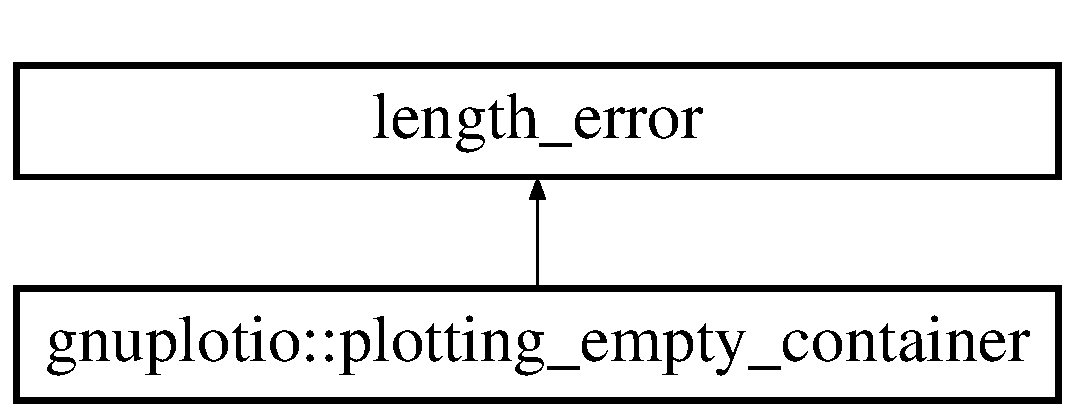
\includegraphics[height=2.000000cm]{classgnuplotio_1_1plotting__empty__container}
\end{center}
\end{figure}
\subsection*{Public Member Functions}
\begin{DoxyCompactItemize}
\item 
\hyperlink{classgnuplotio_1_1plotting__empty__container_ac6498c9ce44e48757444c8335fb544a1}{plotting\+\_\+empty\+\_\+container} ()
\end{DoxyCompactItemize}


\subsection{Detailed Description}


Definition at line 1180 of file gnuplot-\/iostream.\+h.



\subsection{Constructor \& Destructor Documentation}
\index{gnuplotio\+::plotting\+\_\+empty\+\_\+container@{gnuplotio\+::plotting\+\_\+empty\+\_\+container}!plotting\+\_\+empty\+\_\+container@{plotting\+\_\+empty\+\_\+container}}
\index{plotting\+\_\+empty\+\_\+container@{plotting\+\_\+empty\+\_\+container}!gnuplotio\+::plotting\+\_\+empty\+\_\+container@{gnuplotio\+::plotting\+\_\+empty\+\_\+container}}
\subsubsection[{\texorpdfstring{plotting\+\_\+empty\+\_\+container()}{plotting_empty_container()}}]{\setlength{\rightskip}{0pt plus 5cm}gnuplotio\+::plotting\+\_\+empty\+\_\+container\+::plotting\+\_\+empty\+\_\+container (
\begin{DoxyParamCaption}
{}
\end{DoxyParamCaption}
)\hspace{0.3cm}{\ttfamily [inline]}}\hypertarget{classgnuplotio_1_1plotting__empty__container_ac6498c9ce44e48757444c8335fb544a1}{}\label{classgnuplotio_1_1plotting__empty__container_ac6498c9ce44e48757444c8335fb544a1}


Definition at line 1182 of file gnuplot-\/iostream.\+h.



The documentation for this class was generated from the following file\+:\begin{DoxyCompactItemize}
\item 
include/\hyperlink{gnuplot-iostream_8h}{gnuplot-\/iostream.\+h}\end{DoxyCompactItemize}

\hypertarget{class_steer_algorithm}{}\section{Steer\+Algorithm Class Reference}
\label{class_steer_algorithm}\index{Steer\+Algorithm@{Steer\+Algorithm}}


Class \hyperlink{class_steer_algorithm}{Steer\+Algorithm} contains the methods of the Steering Algorithm.  




{\ttfamily \#include $<$Steer\+Algorithm.\+hpp$>$}



Inheritance diagram for Steer\+Algorithm\+:
\nopagebreak
\begin{figure}[H]
\begin{center}
\leavevmode
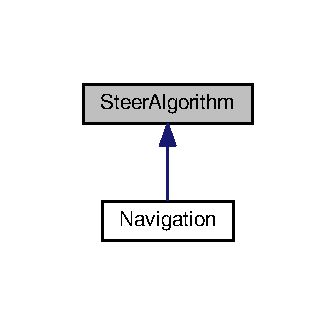
\includegraphics[width=161pt]{class_steer_algorithm__inherit__graph}
\end{center}
\end{figure}
\subsection*{Public Member Functions}
\begin{DoxyCompactItemize}
\item 
\hyperlink{class_steer_algorithm_af64dd94816ab9d00d85227a42b26a3e8}{Steer\+Algorithm} ()\hypertarget{class_steer_algorithm_af64dd94816ab9d00d85227a42b26a3e8}{}\label{class_steer_algorithm_af64dd94816ab9d00d85227a42b26a3e8}

\begin{DoxyCompactList}\small\item\em Constructor of class \hyperlink{class_steer_algorithm}{Steer\+Algorithm}. \end{DoxyCompactList}\item 
\hyperlink{class_steer_algorithm_a37dd2ef0ed856582aaacc103a6cd6700}{$\sim$\+Steer\+Algorithm} ()\hypertarget{class_steer_algorithm_a37dd2ef0ed856582aaacc103a6cd6700}{}\label{class_steer_algorithm_a37dd2ef0ed856582aaacc103a6cd6700}

\begin{DoxyCompactList}\small\item\em Destructor of class \hyperlink{class_steer_algorithm}{Steer\+Algorithm}. \end{DoxyCompactList}\item 
double \hyperlink{class_steer_algorithm_a06a7dd049280fab40d1b54c912daf399}{get\+Corr\+Radius\+\_\+} ()
\begin{DoxyCompactList}\small\item\em Function to get corresponding radius in meters. \end{DoxyCompactList}\item 
bool \hyperlink{class_steer_algorithm_a93cf1fc7d06376ddeaa4e81f2b0a22cc}{set\+Corr\+Radius\+\_\+} (double r)
\begin{DoxyCompactList}\small\item\em Function to set corresponding radius in meters. \end{DoxyCompactList}\item 
double \hyperlink{class_steer_algorithm_a17ff78af17e900f752237d274bcf751d}{arc\+Length} (double diff\+Angle, double corr\+Radius)
\begin{DoxyCompactList}\small\item\em Function to calculate the length of arc in meters to be traced in order to head in target direction. \end{DoxyCompactList}\item 
double \hyperlink{class_steer_algorithm_a6067af69593713f561890ae8ad23f5ff}{change\+Wheel\+Angles} (double corr\+Radius, double shaft\+Length, double shaft\+Distance)
\begin{DoxyCompactList}\small\item\em Function to calculate the angles in degrees for left and right wheels as per ackermann model, and then feed them to corresponding servos. \end{DoxyCompactList}\item 
bool \hyperlink{class_steer_algorithm_ab251b6fd1f88fb7a526b0d55cd12625b}{reset\+Wheel} ()
\begin{DoxyCompactList}\small\item\em Function to set wheel angles to 0. \end{DoxyCompactList}\item 
double \hyperlink{class_steer_algorithm_aefdb433f65c47bf6e0d6af5de98c8f5a}{turn\+Time} (double arclength, double new\+Velocity)
\begin{DoxyCompactList}\small\item\em Function to calculate time in seconds required to turn or keep wheels at the an angle. \end{DoxyCompactList}\end{DoxyCompactItemize}
\subsection*{Public Attributes}
\begin{DoxyCompactItemize}
\item 
const double {\bfseries shaft\+Length} = 4\hypertarget{class_steer_algorithm_a9d5bc20acba39f0e53c3d0f6fc280433}{}\label{class_steer_algorithm_a9d5bc20acba39f0e53c3d0f6fc280433}

\item 
const double {\bfseries shaft\+Distance} = 8\hypertarget{class_steer_algorithm_a38bc87552a30e8eda8f647cf341c9657}{}\label{class_steer_algorithm_a38bc87552a30e8eda8f647cf341c9657}

\item 
const double {\bfseries max\+Turn\+Velocity} = 20\hypertarget{class_steer_algorithm_acfce52839329f0ebb316f633494466e1}{}\label{class_steer_algorithm_acfce52839329f0ebb316f633494466e1}

\item 
double {\bfseries heading}\hypertarget{class_steer_algorithm_ada73b1f087245af5cda5d1d6b9be7d31}{}\label{class_steer_algorithm_ada73b1f087245af5cda5d1d6b9be7d31}

\item 
double {\bfseries target\+Heading}\hypertarget{class_steer_algorithm_a071efeb53e86ee949940b0ab10986044}{}\label{class_steer_algorithm_a071efeb53e86ee949940b0ab10986044}

\item 
int {\bfseries dir}\hypertarget{class_steer_algorithm_af6ad5604b62eec22cc2d385c7683d019}{}\label{class_steer_algorithm_af6ad5604b62eec22cc2d385c7683d019}

\end{DoxyCompactItemize}


\subsection{Detailed Description}
Class \hyperlink{class_steer_algorithm}{Steer\+Algorithm} contains the methods of the Steering Algorithm. 

\subsection{Member Function Documentation}
\index{Steer\+Algorithm@{Steer\+Algorithm}!arc\+Length@{arc\+Length}}
\index{arc\+Length@{arc\+Length}!Steer\+Algorithm@{Steer\+Algorithm}}
\subsubsection[{\texorpdfstring{arc\+Length(double diff\+Angle, double corr\+Radius)}{arcLength(double diffAngle, double corrRadius)}}]{\setlength{\rightskip}{0pt plus 5cm}double Steer\+Algorithm\+::arc\+Length (
\begin{DoxyParamCaption}
\item[{double}]{diff\+Angle, }
\item[{double}]{corr\+Radius}
\end{DoxyParamCaption}
)}\hypertarget{class_steer_algorithm_a17ff78af17e900f752237d274bcf751d}{}\label{class_steer_algorithm_a17ff78af17e900f752237d274bcf751d}


Function to calculate the length of arc in meters to be traced in order to head in target direction. 


\begin{DoxyParams}{Parameters}
{\em double} & diff\+Angle, difference in current and target heading \\
\hline
{\em double} & corr\+Radius, corresponding radius \\
\hline
\end{DoxyParams}
\begin{DoxyReturn}{Returns}
double arclength 
\end{DoxyReturn}
\index{Steer\+Algorithm@{Steer\+Algorithm}!change\+Wheel\+Angles@{change\+Wheel\+Angles}}
\index{change\+Wheel\+Angles@{change\+Wheel\+Angles}!Steer\+Algorithm@{Steer\+Algorithm}}
\subsubsection[{\texorpdfstring{change\+Wheel\+Angles(double corr\+Radius, double shaft\+Length, double shaft\+Distance)}{changeWheelAngles(double corrRadius, double shaftLength, double shaftDistance)}}]{\setlength{\rightskip}{0pt plus 5cm}double Steer\+Algorithm\+::change\+Wheel\+Angles (
\begin{DoxyParamCaption}
\item[{double}]{corr\+Radius, }
\item[{double}]{shaft\+Length, }
\item[{double}]{shaft\+Distance}
\end{DoxyParamCaption}
)}\hypertarget{class_steer_algorithm_a6067af69593713f561890ae8ad23f5ff}{}\label{class_steer_algorithm_a6067af69593713f561890ae8ad23f5ff}


Function to calculate the angles in degrees for left and right wheels as per ackermann model, and then feed them to corresponding servos. 


\begin{DoxyParams}{Parameters}
{\em double} & corr\+Radius, corresponding radius \\
\hline
{\em double} & shaft\+Length, length between wheels \\
\hline
{\em double} & shaf\+Distance, distance between rear and front shaft \\
\hline
\end{DoxyParams}
\begin{DoxyReturn}{Returns}
double max\+Wheel\+Angle 
\end{DoxyReturn}
\index{Steer\+Algorithm@{Steer\+Algorithm}!get\+Corr\+Radius\+\_\+@{get\+Corr\+Radius\+\_\+}}
\index{get\+Corr\+Radius\+\_\+@{get\+Corr\+Radius\+\_\+}!Steer\+Algorithm@{Steer\+Algorithm}}
\subsubsection[{\texorpdfstring{get\+Corr\+Radius\+\_\+()}{getCorrRadius_()}}]{\setlength{\rightskip}{0pt plus 5cm}double Steer\+Algorithm\+::get\+Corr\+Radius\+\_\+ (
\begin{DoxyParamCaption}
{}
\end{DoxyParamCaption}
)}\hypertarget{class_steer_algorithm_a06a7dd049280fab40d1b54c912daf399}{}\label{class_steer_algorithm_a06a7dd049280fab40d1b54c912daf399}


Function to get corresponding radius in meters. 


\begin{DoxyParams}{Parameters}
{\em none} & \\
\hline
\end{DoxyParams}
\begin{DoxyReturn}{Returns}
double corresponding radius 
\end{DoxyReturn}
\index{Steer\+Algorithm@{Steer\+Algorithm}!reset\+Wheel@{reset\+Wheel}}
\index{reset\+Wheel@{reset\+Wheel}!Steer\+Algorithm@{Steer\+Algorithm}}
\subsubsection[{\texorpdfstring{reset\+Wheel()}{resetWheel()}}]{\setlength{\rightskip}{0pt plus 5cm}bool Steer\+Algorithm\+::reset\+Wheel (
\begin{DoxyParamCaption}
{}
\end{DoxyParamCaption}
)}\hypertarget{class_steer_algorithm_ab251b6fd1f88fb7a526b0d55cd12625b}{}\label{class_steer_algorithm_ab251b6fd1f88fb7a526b0d55cd12625b}


Function to set wheel angles to 0. 


\begin{DoxyParams}{Parameters}
{\em none} & \\
\hline
\end{DoxyParams}
\begin{DoxyReturn}{Returns}
bool true 
\end{DoxyReturn}
\index{Steer\+Algorithm@{Steer\+Algorithm}!set\+Corr\+Radius\+\_\+@{set\+Corr\+Radius\+\_\+}}
\index{set\+Corr\+Radius\+\_\+@{set\+Corr\+Radius\+\_\+}!Steer\+Algorithm@{Steer\+Algorithm}}
\subsubsection[{\texorpdfstring{set\+Corr\+Radius\+\_\+(double r)}{setCorrRadius_(double r)}}]{\setlength{\rightskip}{0pt plus 5cm}bool Steer\+Algorithm\+::set\+Corr\+Radius\+\_\+ (
\begin{DoxyParamCaption}
\item[{double}]{r}
\end{DoxyParamCaption}
)}\hypertarget{class_steer_algorithm_a93cf1fc7d06376ddeaa4e81f2b0a22cc}{}\label{class_steer_algorithm_a93cf1fc7d06376ddeaa4e81f2b0a22cc}


Function to set corresponding radius in meters. 


\begin{DoxyParams}{Parameters}
{\em double} & radius \\
\hline
\end{DoxyParams}
\begin{DoxyReturn}{Returns}
bool true 
\end{DoxyReturn}
\index{Steer\+Algorithm@{Steer\+Algorithm}!turn\+Time@{turn\+Time}}
\index{turn\+Time@{turn\+Time}!Steer\+Algorithm@{Steer\+Algorithm}}
\subsubsection[{\texorpdfstring{turn\+Time(double arclength, double new\+Velocity)}{turnTime(double arclength, double newVelocity)}}]{\setlength{\rightskip}{0pt plus 5cm}double Steer\+Algorithm\+::turn\+Time (
\begin{DoxyParamCaption}
\item[{double}]{arclength, }
\item[{double}]{new\+Velocity}
\end{DoxyParamCaption}
)}\hypertarget{class_steer_algorithm_aefdb433f65c47bf6e0d6af5de98c8f5a}{}\label{class_steer_algorithm_aefdb433f65c47bf6e0d6af5de98c8f5a}


Function to calculate time in seconds required to turn or keep wheels at the an angle. 


\begin{DoxyParams}{Parameters}
{\em double} & arc\+Length, length of arc to be traced \\
\hline
{\em double} & new\+Velocity, velocity \\
\hline
\end{DoxyParams}
\begin{DoxyReturn}{Returns}
double time 
\end{DoxyReturn}


The documentation for this class was generated from the following files\+:\begin{DoxyCompactItemize}
\item 
include/\hyperlink{_steer_algorithm_8hpp}{Steer\+Algorithm.\+hpp}\item 
app/\hyperlink{_steer_algorithm_8cpp}{Steer\+Algorithm.\+cpp}\end{DoxyCompactItemize}

\hypertarget{structgnuplotio_1_1_text_sender}{}\section{gnuplotio\+:\+:Text\+Sender$<$ T, Enable $>$ Struct Template Reference}
\label{structgnuplotio_1_1_text_sender}\index{gnuplotio\+::\+Text\+Sender$<$ T, Enable $>$@{gnuplotio\+::\+Text\+Sender$<$ T, Enable $>$}}


{\ttfamily \#include $<$gnuplot-\/iostream.\+h$>$}

\subsection*{Static Public Member Functions}
\begin{DoxyCompactItemize}
\item 
static void \hyperlink{structgnuplotio_1_1_text_sender_a03b58292dc75a4137d30ad7fffd762c6}{send} (std\+::ostream \&stream, const T \&v)
\end{DoxyCompactItemize}


\subsection{Detailed Description}
\subsubsection*{template$<$typename T, typename Enable = void$>$\\*
struct gnuplotio\+::\+Text\+Sender$<$ T, Enable $>$}



Definition at line 433 of file gnuplot-\/iostream.\+h.



\subsection{Member Function Documentation}
\index{gnuplotio\+::\+Text\+Sender@{gnuplotio\+::\+Text\+Sender}!send@{send}}
\index{send@{send}!gnuplotio\+::\+Text\+Sender@{gnuplotio\+::\+Text\+Sender}}
\subsubsection[{\texorpdfstring{send(std\+::ostream \&stream, const T \&v)}{send(std::ostream &stream, const T &v)}}]{\setlength{\rightskip}{0pt plus 5cm}template$<$typename T, typename Enable = void$>$ static void {\bf gnuplotio\+::\+Text\+Sender}$<$ T, Enable $>$\+::send (
\begin{DoxyParamCaption}
\item[{std\+::ostream \&}]{stream, }
\item[{const T \&}]{v}
\end{DoxyParamCaption}
)\hspace{0.3cm}{\ttfamily [inline]}, {\ttfamily [static]}}\hypertarget{structgnuplotio_1_1_text_sender_a03b58292dc75a4137d30ad7fffd762c6}{}\label{structgnuplotio_1_1_text_sender_a03b58292dc75a4137d30ad7fffd762c6}


Definition at line 434 of file gnuplot-\/iostream.\+h.



The documentation for this struct was generated from the following file\+:\begin{DoxyCompactItemize}
\item 
include/\hyperlink{gnuplot-iostream_8h}{gnuplot-\/iostream.\+h}\end{DoxyCompactItemize}

\hypertarget{structgnuplotio_1_1_text_sender_3_01char_01_4}{}\section{gnuplotio\+:\+:Text\+Sender$<$ char $>$ Struct Template Reference}
\label{structgnuplotio_1_1_text_sender_3_01char_01_4}\index{gnuplotio\+::\+Text\+Sender$<$ char $>$@{gnuplotio\+::\+Text\+Sender$<$ char $>$}}


{\ttfamily \#include $<$gnuplot-\/iostream.\+h$>$}

Inheritance diagram for gnuplotio\+:\+:Text\+Sender$<$ char $>$\+:\begin{figure}[H]
\begin{center}
\leavevmode
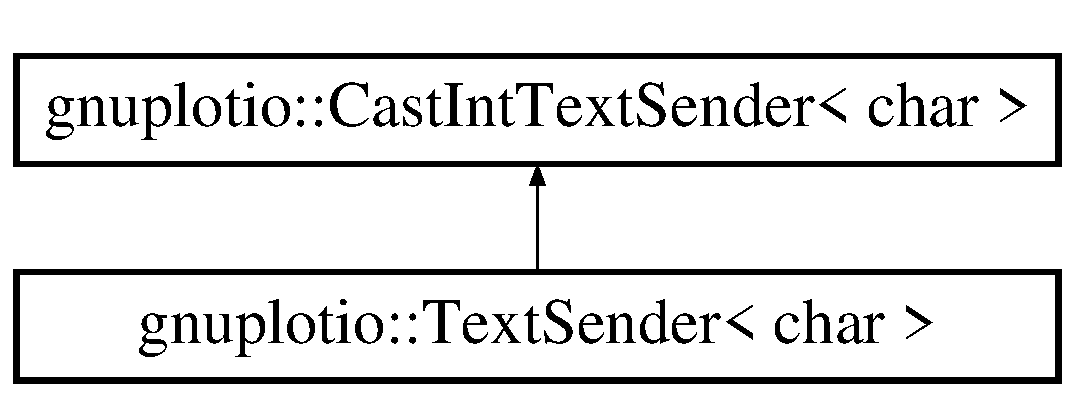
\includegraphics[height=2.000000cm]{structgnuplotio_1_1_text_sender_3_01char_01_4}
\end{center}
\end{figure}
\subsection*{Additional Inherited Members}


\subsection{Detailed Description}
\subsubsection*{template$<$$>$\\*
struct gnuplotio\+::\+Text\+Sender$<$ char $>$}



Definition at line 499 of file gnuplot-\/iostream.\+h.



The documentation for this struct was generated from the following file\+:\begin{DoxyCompactItemize}
\item 
include/\hyperlink{gnuplot-iostream_8h}{gnuplot-\/iostream.\+h}\end{DoxyCompactItemize}

\hypertarget{structgnuplotio_1_1_text_sender_3_01double_01_4}{}\section{gnuplotio\+:\+:Text\+Sender$<$ double $>$ Struct Template Reference}
\label{structgnuplotio_1_1_text_sender_3_01double_01_4}\index{gnuplotio\+::\+Text\+Sender$<$ double $>$@{gnuplotio\+::\+Text\+Sender$<$ double $>$}}


{\ttfamily \#include $<$gnuplot-\/iostream.\+h$>$}

Inheritance diagram for gnuplotio\+:\+:Text\+Sender$<$ double $>$\+:\begin{figure}[H]
\begin{center}
\leavevmode
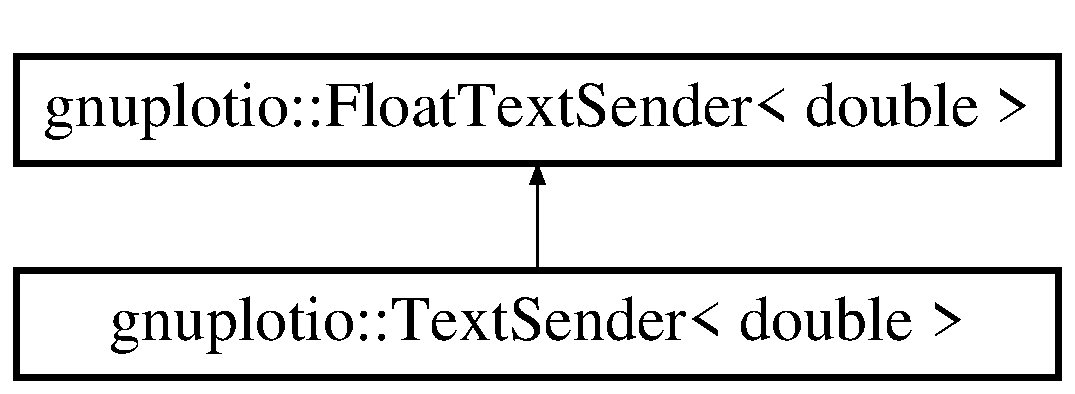
\includegraphics[height=2.000000cm]{structgnuplotio_1_1_text_sender_3_01double_01_4}
\end{center}
\end{figure}
\subsection*{Additional Inherited Members}


\subsection{Detailed Description}
\subsubsection*{template$<$$>$\\*
struct gnuplotio\+::\+Text\+Sender$<$ double $>$}



Definition at line 511 of file gnuplot-\/iostream.\+h.



The documentation for this struct was generated from the following file\+:\begin{DoxyCompactItemize}
\item 
include/\hyperlink{gnuplot-iostream_8h}{gnuplot-\/iostream.\+h}\end{DoxyCompactItemize}

\hypertarget{structgnuplotio_1_1_text_sender_3_01float_01_4}{}\section{gnuplotio\+:\+:Text\+Sender$<$ float $>$ Struct Template Reference}
\label{structgnuplotio_1_1_text_sender_3_01float_01_4}\index{gnuplotio\+::\+Text\+Sender$<$ float $>$@{gnuplotio\+::\+Text\+Sender$<$ float $>$}}


{\ttfamily \#include $<$gnuplot-\/iostream.\+h$>$}

Inheritance diagram for gnuplotio\+:\+:Text\+Sender$<$ float $>$\+:\begin{figure}[H]
\begin{center}
\leavevmode
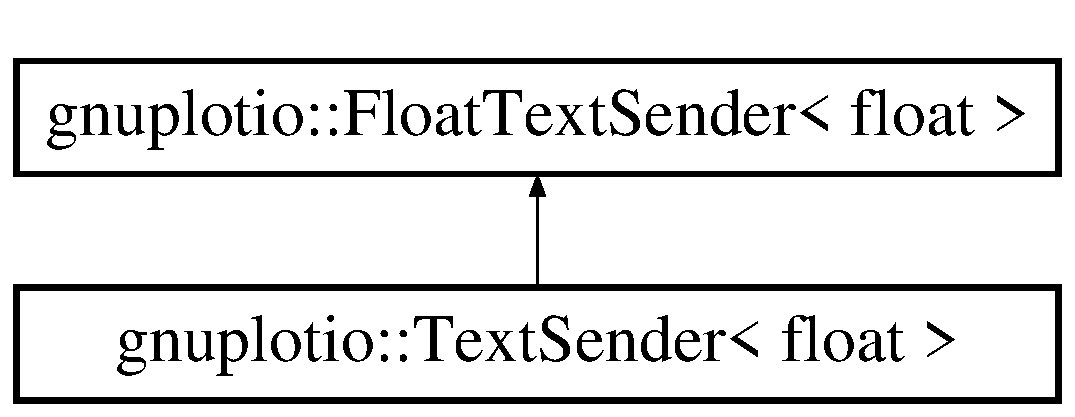
\includegraphics[height=2.000000cm]{structgnuplotio_1_1_text_sender_3_01float_01_4}
\end{center}
\end{figure}
\subsection*{Additional Inherited Members}


\subsection{Detailed Description}
\subsubsection*{template$<$$>$\\*
struct gnuplotio\+::\+Text\+Sender$<$ float $>$}



Definition at line 510 of file gnuplot-\/iostream.\+h.



The documentation for this struct was generated from the following file\+:\begin{DoxyCompactItemize}
\item 
include/\hyperlink{gnuplot-iostream_8h}{gnuplot-\/iostream.\+h}\end{DoxyCompactItemize}

\hypertarget{structgnuplotio_1_1_text_sender_3_01long_01double_01_4}{}\section{gnuplotio\+:\+:Text\+Sender$<$ long double $>$ Struct Template Reference}
\label{structgnuplotio_1_1_text_sender_3_01long_01double_01_4}\index{gnuplotio\+::\+Text\+Sender$<$ long double $>$@{gnuplotio\+::\+Text\+Sender$<$ long double $>$}}


{\ttfamily \#include $<$gnuplot-\/iostream.\+h$>$}

Inheritance diagram for gnuplotio\+:\+:Text\+Sender$<$ long double $>$\+:\begin{figure}[H]
\begin{center}
\leavevmode
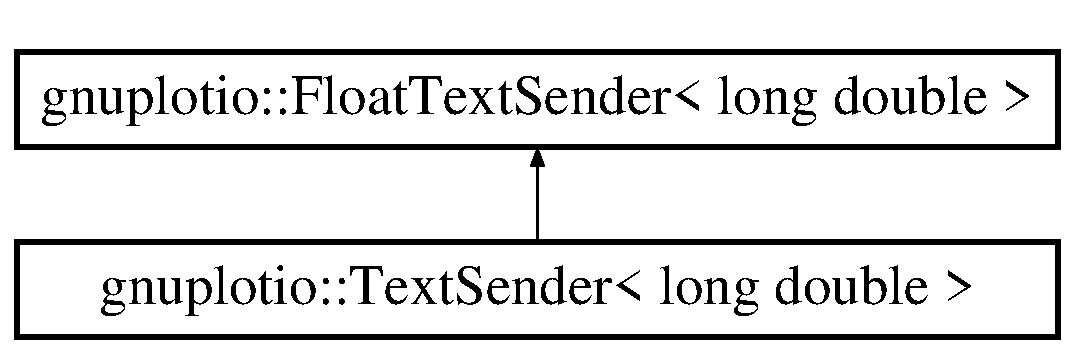
\includegraphics[height=2.000000cm]{structgnuplotio_1_1_text_sender_3_01long_01double_01_4}
\end{center}
\end{figure}
\subsection*{Additional Inherited Members}


\subsection{Detailed Description}
\subsubsection*{template$<$$>$\\*
struct gnuplotio\+::\+Text\+Sender$<$ long double $>$}



Definition at line 512 of file gnuplot-\/iostream.\+h.



The documentation for this struct was generated from the following file\+:\begin{DoxyCompactItemize}
\item 
include/\hyperlink{gnuplot-iostream_8h}{gnuplot-\/iostream.\+h}\end{DoxyCompactItemize}

\hypertarget{structgnuplotio_1_1_text_sender_3_01signed_01char_01_4}{}\section{gnuplotio\+:\+:Text\+Sender$<$ signed char $>$ Struct Template Reference}
\label{structgnuplotio_1_1_text_sender_3_01signed_01char_01_4}\index{gnuplotio\+::\+Text\+Sender$<$ signed char $>$@{gnuplotio\+::\+Text\+Sender$<$ signed char $>$}}


{\ttfamily \#include $<$gnuplot-\/iostream.\+h$>$}

Inheritance diagram for gnuplotio\+:\+:Text\+Sender$<$ signed char $>$\+:\begin{figure}[H]
\begin{center}
\leavevmode
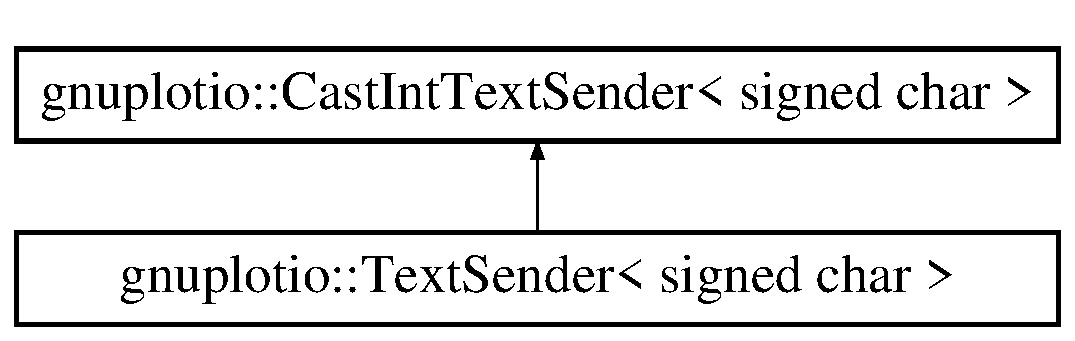
\includegraphics[height=2.000000cm]{structgnuplotio_1_1_text_sender_3_01signed_01char_01_4}
\end{center}
\end{figure}
\subsection*{Additional Inherited Members}


\subsection{Detailed Description}
\subsubsection*{template$<$$>$\\*
struct gnuplotio\+::\+Text\+Sender$<$ signed char $>$}



Definition at line 500 of file gnuplot-\/iostream.\+h.



The documentation for this struct was generated from the following file\+:\begin{DoxyCompactItemize}
\item 
include/\hyperlink{gnuplot-iostream_8h}{gnuplot-\/iostream.\+h}\end{DoxyCompactItemize}

\hypertarget{structgnuplotio_1_1_text_sender_3_01std_1_1complex_3_01_t_01_4_01_4}{}\section{gnuplotio\+:\+:Text\+Sender$<$ std\+:\+:complex$<$ T $>$ $>$ Struct Template Reference}
\label{structgnuplotio_1_1_text_sender_3_01std_1_1complex_3_01_t_01_4_01_4}\index{gnuplotio\+::\+Text\+Sender$<$ std\+::complex$<$ T $>$ $>$@{gnuplotio\+::\+Text\+Sender$<$ std\+::complex$<$ T $>$ $>$}}


{\ttfamily \#include $<$gnuplot-\/iostream.\+h$>$}

\subsection*{Static Public Member Functions}
\begin{DoxyCompactItemize}
\item 
static void \hyperlink{structgnuplotio_1_1_text_sender_3_01std_1_1complex_3_01_t_01_4_01_4_ad524aa3e121d0ebd66346d77f1fd5a1c}{send} (std\+::ostream \&stream, const std\+::complex$<$ T $>$ \&v)
\end{DoxyCompactItemize}


\subsection{Detailed Description}
\subsubsection*{template$<$typename T$>$\\*
struct gnuplotio\+::\+Text\+Sender$<$ std\+::complex$<$ T $>$ $>$}



Definition at line 548 of file gnuplot-\/iostream.\+h.



\subsection{Member Function Documentation}
\index{gnuplotio\+::\+Text\+Sender$<$ std\+::complex$<$ T $>$ $>$@{gnuplotio\+::\+Text\+Sender$<$ std\+::complex$<$ T $>$ $>$}!send@{send}}
\index{send@{send}!gnuplotio\+::\+Text\+Sender$<$ std\+::complex$<$ T $>$ $>$@{gnuplotio\+::\+Text\+Sender$<$ std\+::complex$<$ T $>$ $>$}}
\subsubsection[{\texorpdfstring{send(std\+::ostream \&stream, const std\+::complex$<$ T $>$ \&v)}{send(std::ostream &stream, const std::complex< T > &v)}}]{\setlength{\rightskip}{0pt plus 5cm}template$<$typename T $>$ static void {\bf gnuplotio\+::\+Text\+Sender}$<$ std\+::complex$<$ T $>$ $>$\+::send (
\begin{DoxyParamCaption}
\item[{std\+::ostream \&}]{stream, }
\item[{const std\+::complex$<$ T $>$ \&}]{v}
\end{DoxyParamCaption}
)\hspace{0.3cm}{\ttfamily [inline]}, {\ttfamily [static]}}\hypertarget{structgnuplotio_1_1_text_sender_3_01std_1_1complex_3_01_t_01_4_01_4_ad524aa3e121d0ebd66346d77f1fd5a1c}{}\label{structgnuplotio_1_1_text_sender_3_01std_1_1complex_3_01_t_01_4_01_4_ad524aa3e121d0ebd66346d77f1fd5a1c}


Definition at line 549 of file gnuplot-\/iostream.\+h.



The documentation for this struct was generated from the following file\+:\begin{DoxyCompactItemize}
\item 
include/\hyperlink{gnuplot-iostream_8h}{gnuplot-\/iostream.\+h}\end{DoxyCompactItemize}

\hypertarget{structgnuplotio_1_1_text_sender_3_01std_1_1pair_3_01_t_00_01_u_01_4_01_4}{}\section{gnuplotio\+:\+:Text\+Sender$<$ std\+:\+:pair$<$ T, U $>$ $>$ Struct Template Reference}
\label{structgnuplotio_1_1_text_sender_3_01std_1_1pair_3_01_t_00_01_u_01_4_01_4}\index{gnuplotio\+::\+Text\+Sender$<$ std\+::pair$<$ T, U $>$ $>$@{gnuplotio\+::\+Text\+Sender$<$ std\+::pair$<$ T, U $>$ $>$}}


{\ttfamily \#include $<$gnuplot-\/iostream.\+h$>$}

\subsection*{Static Public Member Functions}
\begin{DoxyCompactItemize}
\item 
static void \hyperlink{structgnuplotio_1_1_text_sender_3_01std_1_1pair_3_01_t_00_01_u_01_4_01_4_ae1f3a6ffd8a60bb73d787578327154d1}{send} (std\+::ostream \&stream, const std\+::pair$<$ T, U $>$ \&v)
\end{DoxyCompactItemize}


\subsection{Detailed Description}
\subsubsection*{template$<$typename T, typename U$>$\\*
struct gnuplotio\+::\+Text\+Sender$<$ std\+::pair$<$ T, U $>$ $>$}



Definition at line 519 of file gnuplot-\/iostream.\+h.



\subsection{Member Function Documentation}
\index{gnuplotio\+::\+Text\+Sender$<$ std\+::pair$<$ T, U $>$ $>$@{gnuplotio\+::\+Text\+Sender$<$ std\+::pair$<$ T, U $>$ $>$}!send@{send}}
\index{send@{send}!gnuplotio\+::\+Text\+Sender$<$ std\+::pair$<$ T, U $>$ $>$@{gnuplotio\+::\+Text\+Sender$<$ std\+::pair$<$ T, U $>$ $>$}}
\subsubsection[{\texorpdfstring{send(std\+::ostream \&stream, const std\+::pair$<$ T, U $>$ \&v)}{send(std::ostream &stream, const std::pair< T, U > &v)}}]{\setlength{\rightskip}{0pt plus 5cm}template$<$typename T , typename U $>$ static void {\bf gnuplotio\+::\+Text\+Sender}$<$ std\+::pair$<$ T, U $>$ $>$\+::send (
\begin{DoxyParamCaption}
\item[{std\+::ostream \&}]{stream, }
\item[{const std\+::pair$<$ T, U $>$ \&}]{v}
\end{DoxyParamCaption}
)\hspace{0.3cm}{\ttfamily [inline]}, {\ttfamily [static]}}\hypertarget{structgnuplotio_1_1_text_sender_3_01std_1_1pair_3_01_t_00_01_u_01_4_01_4_ae1f3a6ffd8a60bb73d787578327154d1}{}\label{structgnuplotio_1_1_text_sender_3_01std_1_1pair_3_01_t_00_01_u_01_4_01_4_ae1f3a6ffd8a60bb73d787578327154d1}


Definition at line 520 of file gnuplot-\/iostream.\+h.



The documentation for this struct was generated from the following file\+:\begin{DoxyCompactItemize}
\item 
include/\hyperlink{gnuplot-iostream_8h}{gnuplot-\/iostream.\+h}\end{DoxyCompactItemize}

\hypertarget{structgnuplotio_1_1_text_sender_3_01_t_00_01typename_01boost_1_1enable__if_3_01boost_1_1mpl_1_1ad1ac3a3da167856c52be6ae54ba2c114}{}\section{gnuplotio\+:\+:Text\+Sender$<$ T, typename boost\+:\+:enable\+\_\+if$<$ boost\+:\+:mpl\+:\+:and\+\_\+$<$ is\+\_\+boost\+\_\+tuple$<$ T $>$, boost\+:\+:mpl\+:\+:not\+\_\+$<$ is\+\_\+boost\+\_\+tuple\+\_\+nulltype$<$ typename T\+:\+:tail\+\_\+type $>$ $>$ $>$ $>$\+:\+:type $>$ Struct Template Reference}
\label{structgnuplotio_1_1_text_sender_3_01_t_00_01typename_01boost_1_1enable__if_3_01boost_1_1mpl_1_1ad1ac3a3da167856c52be6ae54ba2c114}\index{gnuplotio\+::\+Text\+Sender$<$ T, typename boost\+::enable\+\_\+if$<$ boost\+::mpl\+::and\+\_\+$<$ is\+\_\+boost\+\_\+tuple$<$ T $>$, boost\+::mpl\+::not\+\_\+$<$ is\+\_\+boost\+\_\+tuple\+\_\+nulltype$<$ typename T\+::tail\+\_\+type $>$ $>$ $>$ $>$\+::type $>$@{gnuplotio\+::\+Text\+Sender$<$ T, typename boost\+::enable\+\_\+if$<$ boost\+::mpl\+::and\+\_\+$<$ is\+\_\+boost\+\_\+tuple$<$ T $>$, boost\+::mpl\+::not\+\_\+$<$ is\+\_\+boost\+\_\+tuple\+\_\+nulltype$<$ typename T\+::tail\+\_\+type $>$ $>$ $>$ $>$\+::type $>$}}


{\ttfamily \#include $<$gnuplot-\/iostream.\+h$>$}

\subsection*{Static Public Member Functions}
\begin{DoxyCompactItemize}
\item 
static void \hyperlink{structgnuplotio_1_1_text_sender_3_01_t_00_01typename_01boost_1_1enable__if_3_01boost_1_1mpl_1_1ad1ac3a3da167856c52be6ae54ba2c114_a57bf894398f70f08cd4bac18ee5cbf68}{send} (std\+::ostream \&stream, const T \&v)
\end{DoxyCompactItemize}


\subsection{Detailed Description}
\subsubsection*{template$<$typename T$>$\\*
struct gnuplotio\+::\+Text\+Sender$<$ T, typename boost\+::enable\+\_\+if$<$ boost\+::mpl\+::and\+\_\+$<$ is\+\_\+boost\+\_\+tuple$<$ T $>$, boost\+::mpl\+::not\+\_\+$<$ is\+\_\+boost\+\_\+tuple\+\_\+nulltype$<$ typename T\+::tail\+\_\+type $>$ $>$ $>$ $>$\+::type $>$}



Definition at line 577 of file gnuplot-\/iostream.\+h.



\subsection{Member Function Documentation}
\index{gnuplotio\+::\+Text\+Sender$<$ T, typename boost\+::enable\+\_\+if$<$ boost\+::mpl\+::and\+\_\+$<$ is\+\_\+boost\+\_\+tuple$<$ T $>$, boost\+::mpl\+::not\+\_\+$<$ is\+\_\+boost\+\_\+tuple\+\_\+nulltype$<$ typename T\+::tail\+\_\+type $>$ $>$ $>$ $>$\+::type $>$@{gnuplotio\+::\+Text\+Sender$<$ T, typename boost\+::enable\+\_\+if$<$ boost\+::mpl\+::and\+\_\+$<$ is\+\_\+boost\+\_\+tuple$<$ T $>$, boost\+::mpl\+::not\+\_\+$<$ is\+\_\+boost\+\_\+tuple\+\_\+nulltype$<$ typename T\+::tail\+\_\+type $>$ $>$ $>$ $>$\+::type $>$}!send@{send}}
\index{send@{send}!gnuplotio\+::\+Text\+Sender$<$ T, typename boost\+::enable\+\_\+if$<$ boost\+::mpl\+::and\+\_\+$<$ is\+\_\+boost\+\_\+tuple$<$ T $>$, boost\+::mpl\+::not\+\_\+$<$ is\+\_\+boost\+\_\+tuple\+\_\+nulltype$<$ typename T\+::tail\+\_\+type $>$ $>$ $>$ $>$\+::type $>$@{gnuplotio\+::\+Text\+Sender$<$ T, typename boost\+::enable\+\_\+if$<$ boost\+::mpl\+::and\+\_\+$<$ is\+\_\+boost\+\_\+tuple$<$ T $>$, boost\+::mpl\+::not\+\_\+$<$ is\+\_\+boost\+\_\+tuple\+\_\+nulltype$<$ typename T\+::tail\+\_\+type $>$ $>$ $>$ $>$\+::type $>$}}
\subsubsection[{\texorpdfstring{send(std\+::ostream \&stream, const T \&v)}{send(std::ostream &stream, const T &v)}}]{\setlength{\rightskip}{0pt plus 5cm}template$<$typename T $>$ static void {\bf gnuplotio\+::\+Text\+Sender}$<$ T, typename boost\+::enable\+\_\+if$<$ boost\+::mpl\+::and\+\_\+$<$ {\bf is\+\_\+boost\+\_\+tuple}$<$ T $>$, boost\+::mpl\+::not\+\_\+$<$ {\bf is\+\_\+boost\+\_\+tuple\+\_\+nulltype}$<$ typename T\+::tail\+\_\+type $>$ $>$ $>$ $>$\+::type $>$\+::send (
\begin{DoxyParamCaption}
\item[{std\+::ostream \&}]{stream, }
\item[{const T \&}]{v}
\end{DoxyParamCaption}
)\hspace{0.3cm}{\ttfamily [inline]}, {\ttfamily [static]}}\hypertarget{structgnuplotio_1_1_text_sender_3_01_t_00_01typename_01boost_1_1enable__if_3_01boost_1_1mpl_1_1ad1ac3a3da167856c52be6ae54ba2c114_a57bf894398f70f08cd4bac18ee5cbf68}{}\label{structgnuplotio_1_1_text_sender_3_01_t_00_01typename_01boost_1_1enable__if_3_01boost_1_1mpl_1_1ad1ac3a3da167856c52be6ae54ba2c114_a57bf894398f70f08cd4bac18ee5cbf68}


Definition at line 585 of file gnuplot-\/iostream.\+h.



The documentation for this struct was generated from the following file\+:\begin{DoxyCompactItemize}
\item 
include/\hyperlink{gnuplot-iostream_8h}{gnuplot-\/iostream.\+h}\end{DoxyCompactItemize}

\hypertarget{structgnuplotio_1_1_text_sender_3_01_t_00_01typename_01boost_1_1enable__if_3_01boost_1_1mpl_1_1ab6d6864cc1b3ed233c9f15134694f953}{}\section{gnuplotio\+:\+:Text\+Sender$<$ T, typename boost\+:\+:enable\+\_\+if$<$ boost\+:\+:mpl\+:\+:and\+\_\+$<$ is\+\_\+boost\+\_\+tuple$<$ T $>$, is\+\_\+boost\+\_\+tuple\+\_\+nulltype$<$ typename T\+:\+:tail\+\_\+type $>$ $>$ $>$\+:\+:type $>$ Struct Template Reference}
\label{structgnuplotio_1_1_text_sender_3_01_t_00_01typename_01boost_1_1enable__if_3_01boost_1_1mpl_1_1ab6d6864cc1b3ed233c9f15134694f953}\index{gnuplotio\+::\+Text\+Sender$<$ T, typename boost\+::enable\+\_\+if$<$ boost\+::mpl\+::and\+\_\+$<$ is\+\_\+boost\+\_\+tuple$<$ T $>$, is\+\_\+boost\+\_\+tuple\+\_\+nulltype$<$ typename T\+::tail\+\_\+type $>$ $>$ $>$\+::type $>$@{gnuplotio\+::\+Text\+Sender$<$ T, typename boost\+::enable\+\_\+if$<$ boost\+::mpl\+::and\+\_\+$<$ is\+\_\+boost\+\_\+tuple$<$ T $>$, is\+\_\+boost\+\_\+tuple\+\_\+nulltype$<$ typename T\+::tail\+\_\+type $>$ $>$ $>$\+::type $>$}}


{\ttfamily \#include $<$gnuplot-\/iostream.\+h$>$}

\subsection*{Static Public Member Functions}
\begin{DoxyCompactItemize}
\item 
static void \hyperlink{structgnuplotio_1_1_text_sender_3_01_t_00_01typename_01boost_1_1enable__if_3_01boost_1_1mpl_1_1ab6d6864cc1b3ed233c9f15134694f953_a76a476180ea04c950c1cfdb71c556525}{send} (std\+::ostream \&stream, const T \&v)
\end{DoxyCompactItemize}


\subsection{Detailed Description}
\subsubsection*{template$<$typename T$>$\\*
struct gnuplotio\+::\+Text\+Sender$<$ T, typename boost\+::enable\+\_\+if$<$ boost\+::mpl\+::and\+\_\+$<$ is\+\_\+boost\+\_\+tuple$<$ T $>$, is\+\_\+boost\+\_\+tuple\+\_\+nulltype$<$ typename T\+::tail\+\_\+type $>$ $>$ $>$\+::type $>$}



Definition at line 593 of file gnuplot-\/iostream.\+h.



\subsection{Member Function Documentation}
\index{gnuplotio\+::\+Text\+Sender$<$ T, typename boost\+::enable\+\_\+if$<$ boost\+::mpl\+::and\+\_\+$<$ is\+\_\+boost\+\_\+tuple$<$ T $>$, is\+\_\+boost\+\_\+tuple\+\_\+nulltype$<$ typename T\+::tail\+\_\+type $>$ $>$ $>$\+::type $>$@{gnuplotio\+::\+Text\+Sender$<$ T, typename boost\+::enable\+\_\+if$<$ boost\+::mpl\+::and\+\_\+$<$ is\+\_\+boost\+\_\+tuple$<$ T $>$, is\+\_\+boost\+\_\+tuple\+\_\+nulltype$<$ typename T\+::tail\+\_\+type $>$ $>$ $>$\+::type $>$}!send@{send}}
\index{send@{send}!gnuplotio\+::\+Text\+Sender$<$ T, typename boost\+::enable\+\_\+if$<$ boost\+::mpl\+::and\+\_\+$<$ is\+\_\+boost\+\_\+tuple$<$ T $>$, is\+\_\+boost\+\_\+tuple\+\_\+nulltype$<$ typename T\+::tail\+\_\+type $>$ $>$ $>$\+::type $>$@{gnuplotio\+::\+Text\+Sender$<$ T, typename boost\+::enable\+\_\+if$<$ boost\+::mpl\+::and\+\_\+$<$ is\+\_\+boost\+\_\+tuple$<$ T $>$, is\+\_\+boost\+\_\+tuple\+\_\+nulltype$<$ typename T\+::tail\+\_\+type $>$ $>$ $>$\+::type $>$}}
\subsubsection[{\texorpdfstring{send(std\+::ostream \&stream, const T \&v)}{send(std::ostream &stream, const T &v)}}]{\setlength{\rightskip}{0pt plus 5cm}template$<$typename T $>$ static void {\bf gnuplotio\+::\+Text\+Sender}$<$ T, typename boost\+::enable\+\_\+if$<$ boost\+::mpl\+::and\+\_\+$<$ {\bf is\+\_\+boost\+\_\+tuple}$<$ T $>$, {\bf is\+\_\+boost\+\_\+tuple\+\_\+nulltype}$<$ typename T\+::tail\+\_\+type $>$ $>$ $>$\+::type $>$\+::send (
\begin{DoxyParamCaption}
\item[{std\+::ostream \&}]{stream, }
\item[{const T \&}]{v}
\end{DoxyParamCaption}
)\hspace{0.3cm}{\ttfamily [inline]}, {\ttfamily [static]}}\hypertarget{structgnuplotio_1_1_text_sender_3_01_t_00_01typename_01boost_1_1enable__if_3_01boost_1_1mpl_1_1ab6d6864cc1b3ed233c9f15134694f953_a76a476180ea04c950c1cfdb71c556525}{}\label{structgnuplotio_1_1_text_sender_3_01_t_00_01typename_01boost_1_1enable__if_3_01boost_1_1mpl_1_1ab6d6864cc1b3ed233c9f15134694f953_a76a476180ea04c950c1cfdb71c556525}


Definition at line 601 of file gnuplot-\/iostream.\+h.



The documentation for this struct was generated from the following file\+:\begin{DoxyCompactItemize}
\item 
include/\hyperlink{gnuplot-iostream_8h}{gnuplot-\/iostream.\+h}\end{DoxyCompactItemize}

\hypertarget{structgnuplotio_1_1_text_sender_3_01unsigned_01char_01_4}{}\section{gnuplotio\+:\+:Text\+Sender$<$ unsigned char $>$ Struct Template Reference}
\label{structgnuplotio_1_1_text_sender_3_01unsigned_01char_01_4}\index{gnuplotio\+::\+Text\+Sender$<$ unsigned char $>$@{gnuplotio\+::\+Text\+Sender$<$ unsigned char $>$}}


{\ttfamily \#include $<$gnuplot-\/iostream.\+h$>$}

Inheritance diagram for gnuplotio\+:\+:Text\+Sender$<$ unsigned char $>$\+:\begin{figure}[H]
\begin{center}
\leavevmode
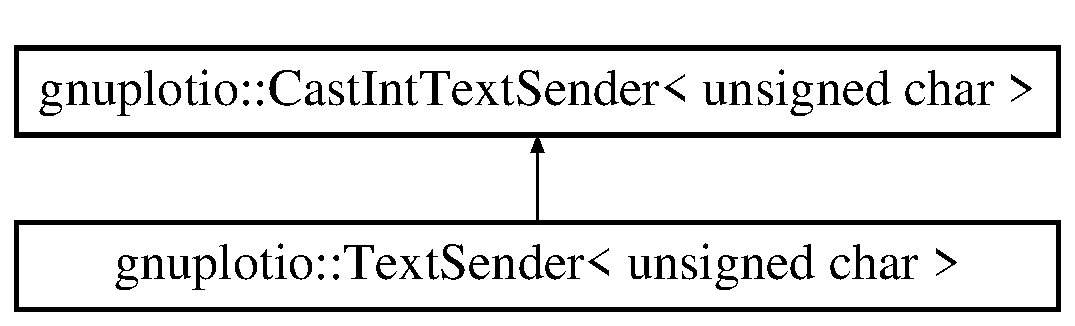
\includegraphics[height=2.000000cm]{structgnuplotio_1_1_text_sender_3_01unsigned_01char_01_4}
\end{center}
\end{figure}
\subsection*{Additional Inherited Members}


\subsection{Detailed Description}
\subsubsection*{template$<$$>$\\*
struct gnuplotio\+::\+Text\+Sender$<$ unsigned char $>$}



Definition at line 501 of file gnuplot-\/iostream.\+h.



The documentation for this struct was generated from the following file\+:\begin{DoxyCompactItemize}
\item 
include/\hyperlink{gnuplot-iostream_8h}{gnuplot-\/iostream.\+h}\end{DoxyCompactItemize}

\hypertarget{structgnuplotio_1_1_mode_auto_decoder_3_01_t_00_01typename_01boost_1_1enable__if__c_3_01_07_arraea646779afc1e35efaeffcebe81e18a0}{}\section{gnuplotio\+:\+:type$<$ T $>$ Struct Template Reference}
\label{structgnuplotio_1_1_mode_auto_decoder_3_01_t_00_01typename_01boost_1_1enable__if__c_3_01_07_arraea646779afc1e35efaeffcebe81e18a0}\index{gnuplotio\+::type$<$ T $>$@{gnuplotio\+::type$<$ T $>$}}


{\ttfamily \#include $<$gnuplot-\/iostream.\+h$>$}

\subsection*{Public Types}
\begin{DoxyCompactItemize}
\item 
typedef \hyperlink{structgnuplotio_1_1_mode1_d}{Mode1D} \hyperlink{structgnuplotio_1_1_mode_auto_decoder_3_01_t_00_01typename_01boost_1_1enable__if__c_3_01_07_arraea646779afc1e35efaeffcebe81e18a0_a17dc2e2ec9d21833a8bd6f1a67e32e48}{mode}
\end{DoxyCompactItemize}


\subsection{Detailed Description}
\subsubsection*{template$<$typename T$>$\\*
struct gnuplotio\+::type$<$ T $>$}



Definition at line 1227 of file gnuplot-\/iostream.\+h.



\subsection{Member Typedef Documentation}
\index{gnuplotio\+::\+Mode\+Auto\+Decoder$<$ T, typename boost\+::enable\+\_\+if\+\_\+c$<$ (\+Array\+Traits$<$ T $>$\+::depth==1) $>$\+::type@{gnuplotio\+::\+Mode\+Auto\+Decoder$<$ T, typename boost\+::enable\+\_\+if\+\_\+c$<$ (\+Array\+Traits$<$ T $>$\+::depth==1) $>$\+::type}!mode@{mode}}
\index{mode@{mode}!gnuplotio\+::\+Mode\+Auto\+Decoder$<$ T, typename boost\+::enable\+\_\+if\+\_\+c$<$ (\+Array\+Traits$<$ T $>$\+::depth==1) $>$\+::type@{gnuplotio\+::\+Mode\+Auto\+Decoder$<$ T, typename boost\+::enable\+\_\+if\+\_\+c$<$ (\+Array\+Traits$<$ T $>$\+::depth==1) $>$\+::type}}
\subsubsection[{\texorpdfstring{mode}{mode}}]{\setlength{\rightskip}{0pt plus 5cm}template$<$typename T $>$ typedef {\bf Mode1D} gnuplotio\+::type$<$ T $>$\+::{\bf mode}}\hypertarget{structgnuplotio_1_1_mode_auto_decoder_3_01_t_00_01typename_01boost_1_1enable__if__c_3_01_07_arraea646779afc1e35efaeffcebe81e18a0_a17dc2e2ec9d21833a8bd6f1a67e32e48}{}\label{structgnuplotio_1_1_mode_auto_decoder_3_01_t_00_01typename_01boost_1_1enable__if__c_3_01_07_arraea646779afc1e35efaeffcebe81e18a0_a17dc2e2ec9d21833a8bd6f1a67e32e48}


Definition at line 1232 of file gnuplot-\/iostream.\+h.



The documentation for this struct was generated from the following file\+:\begin{DoxyCompactItemize}
\item 
include/\hyperlink{gnuplot-iostream_8h}{gnuplot-\/iostream.\+h}\end{DoxyCompactItemize}

\hypertarget{structgnuplotio_1_1_mode_auto_decoder_3_01_t_00_01typename_01boost_1_1enable__if__c_3_01_07_arra8faa7fb46cef74a29a23f22c000e4a99}{}\section{gnuplotio\+:\+:type$<$ T $>$ Struct Template Reference}
\label{structgnuplotio_1_1_mode_auto_decoder_3_01_t_00_01typename_01boost_1_1enable__if__c_3_01_07_arra8faa7fb46cef74a29a23f22c000e4a99}\index{gnuplotio\+::type$<$ T $>$@{gnuplotio\+::type$<$ T $>$}}


{\ttfamily \#include $<$gnuplot-\/iostream.\+h$>$}

\subsection*{Public Types}
\begin{DoxyCompactItemize}
\item 
typedef \hyperlink{structgnuplotio_1_1_mode1_d_unwrap}{Mode1\+D\+Unwrap} \hyperlink{structgnuplotio_1_1_mode_auto_decoder_3_01_t_00_01typename_01boost_1_1enable__if__c_3_01_07_arra8faa7fb46cef74a29a23f22c000e4a99_a9c16f714b67e1c4b38e5c7ff956e8acc}{mode}
\end{DoxyCompactItemize}


\subsection{Detailed Description}
\subsubsection*{template$<$typename T$>$\\*
struct gnuplotio\+::type$<$ T $>$}



Definition at line 1246 of file gnuplot-\/iostream.\+h.



\subsection{Member Typedef Documentation}
\index{gnuplotio\+::\+Mode\+Auto\+Decoder$<$ T, typename boost\+::enable\+\_\+if\+\_\+c$<$ (\+Array\+Traits$<$ T $>$\+::depth==2)\&\&\+Array\+Traits$<$ T $>$\+::allow\+\_\+auto\+\_\+unwrap $>$\+::type@{gnuplotio\+::\+Mode\+Auto\+Decoder$<$ T, typename boost\+::enable\+\_\+if\+\_\+c$<$ (\+Array\+Traits$<$ T $>$\+::depth==2)\&\&\+Array\+Traits$<$ T $>$\+::allow\+\_\+auto\+\_\+unwrap $>$\+::type}!mode@{mode}}
\index{mode@{mode}!gnuplotio\+::\+Mode\+Auto\+Decoder$<$ T, typename boost\+::enable\+\_\+if\+\_\+c$<$ (\+Array\+Traits$<$ T $>$\+::depth==2)\&\&\+Array\+Traits$<$ T $>$\+::allow\+\_\+auto\+\_\+unwrap $>$\+::type@{gnuplotio\+::\+Mode\+Auto\+Decoder$<$ T, typename boost\+::enable\+\_\+if\+\_\+c$<$ (\+Array\+Traits$<$ T $>$\+::depth==2)\&\&\+Array\+Traits$<$ T $>$\+::allow\+\_\+auto\+\_\+unwrap $>$\+::type}}
\subsubsection[{\texorpdfstring{mode}{mode}}]{\setlength{\rightskip}{0pt plus 5cm}template$<$typename T $>$ typedef {\bf Mode1\+D\+Unwrap} gnuplotio\+::type$<$ T $>$\+::{\bf mode}}\hypertarget{structgnuplotio_1_1_mode_auto_decoder_3_01_t_00_01typename_01boost_1_1enable__if__c_3_01_07_arra8faa7fb46cef74a29a23f22c000e4a99_a9c16f714b67e1c4b38e5c7ff956e8acc}{}\label{structgnuplotio_1_1_mode_auto_decoder_3_01_t_00_01typename_01boost_1_1enable__if__c_3_01_07_arra8faa7fb46cef74a29a23f22c000e4a99_a9c16f714b67e1c4b38e5c7ff956e8acc}


Definition at line 1252 of file gnuplot-\/iostream.\+h.



The documentation for this struct was generated from the following file\+:\begin{DoxyCompactItemize}
\item 
include/\hyperlink{gnuplot-iostream_8h}{gnuplot-\/iostream.\+h}\end{DoxyCompactItemize}

\hypertarget{structgnuplotio_1_1_mode_auto_decoder_3_01_t_00_01typename_01boost_1_1enable__if__c_3_01_07_arra33ab7f3325313485a7f29355d9a819fc}{}\section{gnuplotio\+:\+:type$<$ T $>$ Struct Template Reference}
\label{structgnuplotio_1_1_mode_auto_decoder_3_01_t_00_01typename_01boost_1_1enable__if__c_3_01_07_arra33ab7f3325313485a7f29355d9a819fc}\index{gnuplotio\+::type$<$ T $>$@{gnuplotio\+::type$<$ T $>$}}


{\ttfamily \#include $<$gnuplot-\/iostream.\+h$>$}

\subsection*{Public Types}
\begin{DoxyCompactItemize}
\item 
typedef \hyperlink{structgnuplotio_1_1_mode2_d}{Mode2D} \hyperlink{structgnuplotio_1_1_mode_auto_decoder_3_01_t_00_01typename_01boost_1_1enable__if__c_3_01_07_arra33ab7f3325313485a7f29355d9a819fc_a1574a7286cee13eedaeca8f40e7d0527}{mode}
\end{DoxyCompactItemize}


\subsection{Detailed Description}
\subsubsection*{template$<$typename T$>$\\*
struct gnuplotio\+::type$<$ T $>$}



Definition at line 1236 of file gnuplot-\/iostream.\+h.



\subsection{Member Typedef Documentation}
\index{gnuplotio\+::\+Mode\+Auto\+Decoder$<$ T, typename boost\+::enable\+\_\+if\+\_\+c$<$ (\+Array\+Traits$<$ T $>$\+::depth==2)\&\&"!Array\+Traits$<$ T $>$\+::allow\+\_\+auto\+\_\+unwrap $>$\+::type@{gnuplotio\+::\+Mode\+Auto\+Decoder$<$ T, typename boost\+::enable\+\_\+if\+\_\+c$<$ (\+Array\+Traits$<$ T $>$\+::depth==2)\&\&"!Array\+Traits$<$ T $>$\+::allow\+\_\+auto\+\_\+unwrap $>$\+::type}!mode@{mode}}
\index{mode@{mode}!gnuplotio\+::\+Mode\+Auto\+Decoder$<$ T, typename boost\+::enable\+\_\+if\+\_\+c$<$ (\+Array\+Traits$<$ T $>$\+::depth==2)\&\&"!Array\+Traits$<$ T $>$\+::allow\+\_\+auto\+\_\+unwrap $>$\+::type@{gnuplotio\+::\+Mode\+Auto\+Decoder$<$ T, typename boost\+::enable\+\_\+if\+\_\+c$<$ (\+Array\+Traits$<$ T $>$\+::depth==2)\&\&"!Array\+Traits$<$ T $>$\+::allow\+\_\+auto\+\_\+unwrap $>$\+::type}}
\subsubsection[{\texorpdfstring{mode}{mode}}]{\setlength{\rightskip}{0pt plus 5cm}template$<$typename T $>$ typedef {\bf Mode2D} gnuplotio\+::type$<$ T $>$\+::{\bf mode}}\hypertarget{structgnuplotio_1_1_mode_auto_decoder_3_01_t_00_01typename_01boost_1_1enable__if__c_3_01_07_arra33ab7f3325313485a7f29355d9a819fc_a1574a7286cee13eedaeca8f40e7d0527}{}\label{structgnuplotio_1_1_mode_auto_decoder_3_01_t_00_01typename_01boost_1_1enable__if__c_3_01_07_arra33ab7f3325313485a7f29355d9a819fc_a1574a7286cee13eedaeca8f40e7d0527}


Definition at line 1242 of file gnuplot-\/iostream.\+h.



The documentation for this struct was generated from the following file\+:\begin{DoxyCompactItemize}
\item 
include/\hyperlink{gnuplot-iostream_8h}{gnuplot-\/iostream.\+h}\end{DoxyCompactItemize}

\hypertarget{classgnuplotio_1_1_vec_of_range}{}\section{gnuplotio\+:\+:Vec\+Of\+Range$<$ RT $>$ Class Template Reference}
\label{classgnuplotio_1_1_vec_of_range}\index{gnuplotio\+::\+Vec\+Of\+Range$<$ R\+T $>$@{gnuplotio\+::\+Vec\+Of\+Range$<$ R\+T $>$}}


{\ttfamily \#include $<$gnuplot-\/iostream.\+h$>$}

\subsection*{Public Types}
\begin{DoxyCompactItemize}
\item 
typedef std\+::vector$<$ typename R\+T\+::value\+\_\+type $>$ \hyperlink{classgnuplotio_1_1_vec_of_range_aed503f2f8d8ed71b303f2db26872bafd}{value\+\_\+type}
\item 
typedef \hyperlink{classgnuplotio_1_1_vec_of_range}{Vec\+Of\+Range}$<$ typename R\+T\+::subiter\+\_\+type $>$ \hyperlink{classgnuplotio_1_1_vec_of_range_a4cfae20b9797febceffafec3415b52db}{subiter\+\_\+type}
\end{DoxyCompactItemize}
\subsection*{Public Member Functions}
\begin{DoxyCompactItemize}
\item 
\hyperlink{classgnuplotio_1_1_vec_of_range_a077cf69b9ea96d4f0da78a5e72ab2427}{Vec\+Of\+Range} ()
\item 
\hyperlink{classgnuplotio_1_1_vec_of_range_a81e04f9ab4b8641d69df61f695e97e34}{Vec\+Of\+Range} (const std\+::vector$<$ RT $>$ \&\+\_\+rvec)
\item 
bool \hyperlink{classgnuplotio_1_1_vec_of_range_a2beef61aa5b150db9af86b1de2edcb22}{is\+\_\+end} () const 
\item 
void \hyperlink{classgnuplotio_1_1_vec_of_range_a2e5371ab6c88994e3fc6f12324783e1c}{inc} ()
\item 
\hyperlink{classgnuplotio_1_1_vec_of_range_aed503f2f8d8ed71b303f2db26872bafd}{value\+\_\+type} \hyperlink{classgnuplotio_1_1_vec_of_range_aa33d4275110fb0d5d76f56199381740f}{deref} () const 
\item 
\hyperlink{classgnuplotio_1_1_vec_of_range_a4cfae20b9797febceffafec3415b52db}{subiter\+\_\+type} \hyperlink{classgnuplotio_1_1_vec_of_range_a2f2ff571b1ef737f60bb0094e1dc221e}{deref\+\_\+subiter} () const 
\end{DoxyCompactItemize}
\subsection*{Static Public Attributes}
\begin{DoxyCompactItemize}
\item 
static const bool \hyperlink{classgnuplotio_1_1_vec_of_range_a8725d4907d46575dddb7152f1f1d1f66}{is\+\_\+container} = R\+T\+::is\+\_\+container
\item 
static const bool \hyperlink{classgnuplotio_1_1_vec_of_range_a19d87e61a7854f9e22d3dd8a94f79500}{allow\+\_\+auto\+\_\+unwrap} = false
\end{DoxyCompactItemize}
\subsection*{Friends}
\begin{DoxyCompactItemize}
\item 
{\footnotesize template$<$typename T , typename Print\+Mode $>$ }\\void \hyperlink{classgnuplotio_1_1_vec_of_range_adafbfb0122b8e499d1af9c246f4ac288}{deref\+\_\+and\+\_\+print} (std\+::ostream \&, const \hyperlink{classgnuplotio_1_1_vec_of_range}{Vec\+Of\+Range}$<$ T $>$ \&, Print\+Mode)
\end{DoxyCompactItemize}


\subsection{Detailed Description}
\subsubsection*{template$<$typename RT$>$\\*
class gnuplotio\+::\+Vec\+Of\+Range$<$ R\+T $>$}



Definition at line 1096 of file gnuplot-\/iostream.\+h.



\subsection{Member Typedef Documentation}
\index{gnuplotio\+::\+Vec\+Of\+Range@{gnuplotio\+::\+Vec\+Of\+Range}!subiter\+\_\+type@{subiter\+\_\+type}}
\index{subiter\+\_\+type@{subiter\+\_\+type}!gnuplotio\+::\+Vec\+Of\+Range@{gnuplotio\+::\+Vec\+Of\+Range}}
\subsubsection[{\texorpdfstring{subiter\+\_\+type}{subiter_type}}]{\setlength{\rightskip}{0pt plus 5cm}template$<$typename RT$>$ typedef {\bf Vec\+Of\+Range}$<$typename R\+T\+::subiter\+\_\+type$>$ {\bf gnuplotio\+::\+Vec\+Of\+Range}$<$ RT $>$\+::{\bf subiter\+\_\+type}}\hypertarget{classgnuplotio_1_1_vec_of_range_a4cfae20b9797febceffafec3415b52db}{}\label{classgnuplotio_1_1_vec_of_range_a4cfae20b9797febceffafec3415b52db}


Definition at line 1109 of file gnuplot-\/iostream.\+h.

\index{gnuplotio\+::\+Vec\+Of\+Range@{gnuplotio\+::\+Vec\+Of\+Range}!value\+\_\+type@{value\+\_\+type}}
\index{value\+\_\+type@{value\+\_\+type}!gnuplotio\+::\+Vec\+Of\+Range@{gnuplotio\+::\+Vec\+Of\+Range}}
\subsubsection[{\texorpdfstring{value\+\_\+type}{value_type}}]{\setlength{\rightskip}{0pt plus 5cm}template$<$typename RT$>$ typedef std\+::vector$<$typename R\+T\+::value\+\_\+type$>$ {\bf gnuplotio\+::\+Vec\+Of\+Range}$<$ RT $>$\+::{\bf value\+\_\+type}}\hypertarget{classgnuplotio_1_1_vec_of_range_aed503f2f8d8ed71b303f2db26872bafd}{}\label{classgnuplotio_1_1_vec_of_range_aed503f2f8d8ed71b303f2db26872bafd}


Definition at line 1108 of file gnuplot-\/iostream.\+h.



\subsection{Constructor \& Destructor Documentation}
\index{gnuplotio\+::\+Vec\+Of\+Range@{gnuplotio\+::\+Vec\+Of\+Range}!Vec\+Of\+Range@{Vec\+Of\+Range}}
\index{Vec\+Of\+Range@{Vec\+Of\+Range}!gnuplotio\+::\+Vec\+Of\+Range@{gnuplotio\+::\+Vec\+Of\+Range}}
\subsubsection[{\texorpdfstring{Vec\+Of\+Range()}{VecOfRange()}}]{\setlength{\rightskip}{0pt plus 5cm}template$<$typename RT$>$ {\bf gnuplotio\+::\+Vec\+Of\+Range}$<$ RT $>$\+::{\bf Vec\+Of\+Range} (
\begin{DoxyParamCaption}
{}
\end{DoxyParamCaption}
)\hspace{0.3cm}{\ttfamily [inline]}}\hypertarget{classgnuplotio_1_1_vec_of_range_a077cf69b9ea96d4f0da78a5e72ab2427}{}\label{classgnuplotio_1_1_vec_of_range_a077cf69b9ea96d4f0da78a5e72ab2427}


Definition at line 1101 of file gnuplot-\/iostream.\+h.

\index{gnuplotio\+::\+Vec\+Of\+Range@{gnuplotio\+::\+Vec\+Of\+Range}!Vec\+Of\+Range@{Vec\+Of\+Range}}
\index{Vec\+Of\+Range@{Vec\+Of\+Range}!gnuplotio\+::\+Vec\+Of\+Range@{gnuplotio\+::\+Vec\+Of\+Range}}
\subsubsection[{\texorpdfstring{Vec\+Of\+Range(const std\+::vector$<$ R\+T $>$ \&\+\_\+rvec)}{VecOfRange(const std::vector< RT > &_rvec)}}]{\setlength{\rightskip}{0pt plus 5cm}template$<$typename RT$>$ {\bf gnuplotio\+::\+Vec\+Of\+Range}$<$ RT $>$\+::{\bf Vec\+Of\+Range} (
\begin{DoxyParamCaption}
\item[{const std\+::vector$<$ RT $>$ \&}]{\+\_\+rvec}
\end{DoxyParamCaption}
)\hspace{0.3cm}{\ttfamily [inline]}, {\ttfamily [explicit]}}\hypertarget{classgnuplotio_1_1_vec_of_range_a81e04f9ab4b8641d69df61f695e97e34}{}\label{classgnuplotio_1_1_vec_of_range_a81e04f9ab4b8641d69df61f695e97e34}


Definition at line 1102 of file gnuplot-\/iostream.\+h.



\subsection{Member Function Documentation}
\index{gnuplotio\+::\+Vec\+Of\+Range@{gnuplotio\+::\+Vec\+Of\+Range}!deref@{deref}}
\index{deref@{deref}!gnuplotio\+::\+Vec\+Of\+Range@{gnuplotio\+::\+Vec\+Of\+Range}}
\subsubsection[{\texorpdfstring{deref() const }{deref() const }}]{\setlength{\rightskip}{0pt plus 5cm}template$<$typename RT$>$ {\bf value\+\_\+type} {\bf gnuplotio\+::\+Vec\+Of\+Range}$<$ RT $>$\+::deref (
\begin{DoxyParamCaption}
{}
\end{DoxyParamCaption}
) const\hspace{0.3cm}{\ttfamily [inline]}}\hypertarget{classgnuplotio_1_1_vec_of_range_aa33d4275110fb0d5d76f56199381740f}{}\label{classgnuplotio_1_1_vec_of_range_aa33d4275110fb0d5d76f56199381740f}


Definition at line 1128 of file gnuplot-\/iostream.\+h.

\index{gnuplotio\+::\+Vec\+Of\+Range@{gnuplotio\+::\+Vec\+Of\+Range}!deref\+\_\+subiter@{deref\+\_\+subiter}}
\index{deref\+\_\+subiter@{deref\+\_\+subiter}!gnuplotio\+::\+Vec\+Of\+Range@{gnuplotio\+::\+Vec\+Of\+Range}}
\subsubsection[{\texorpdfstring{deref\+\_\+subiter() const }{deref_subiter() const }}]{\setlength{\rightskip}{0pt plus 5cm}template$<$typename RT$>$ {\bf subiter\+\_\+type} {\bf gnuplotio\+::\+Vec\+Of\+Range}$<$ RT $>$\+::deref\+\_\+subiter (
\begin{DoxyParamCaption}
{}
\end{DoxyParamCaption}
) const\hspace{0.3cm}{\ttfamily [inline]}}\hypertarget{classgnuplotio_1_1_vec_of_range_a2f2ff571b1ef737f60bb0094e1dc221e}{}\label{classgnuplotio_1_1_vec_of_range_a2f2ff571b1ef737f60bb0094e1dc221e}


Definition at line 1136 of file gnuplot-\/iostream.\+h.

\index{gnuplotio\+::\+Vec\+Of\+Range@{gnuplotio\+::\+Vec\+Of\+Range}!inc@{inc}}
\index{inc@{inc}!gnuplotio\+::\+Vec\+Of\+Range@{gnuplotio\+::\+Vec\+Of\+Range}}
\subsubsection[{\texorpdfstring{inc()}{inc()}}]{\setlength{\rightskip}{0pt plus 5cm}template$<$typename RT$>$ void {\bf gnuplotio\+::\+Vec\+Of\+Range}$<$ RT $>$\+::inc (
\begin{DoxyParamCaption}
{}
\end{DoxyParamCaption}
)\hspace{0.3cm}{\ttfamily [inline]}}\hypertarget{classgnuplotio_1_1_vec_of_range_a2e5371ab6c88994e3fc6f12324783e1c}{}\label{classgnuplotio_1_1_vec_of_range_a2e5371ab6c88994e3fc6f12324783e1c}


Definition at line 1122 of file gnuplot-\/iostream.\+h.

\index{gnuplotio\+::\+Vec\+Of\+Range@{gnuplotio\+::\+Vec\+Of\+Range}!is\+\_\+end@{is\+\_\+end}}
\index{is\+\_\+end@{is\+\_\+end}!gnuplotio\+::\+Vec\+Of\+Range@{gnuplotio\+::\+Vec\+Of\+Range}}
\subsubsection[{\texorpdfstring{is\+\_\+end() const }{is_end() const }}]{\setlength{\rightskip}{0pt plus 5cm}template$<$typename RT$>$ bool {\bf gnuplotio\+::\+Vec\+Of\+Range}$<$ RT $>$\+::is\+\_\+end (
\begin{DoxyParamCaption}
{}
\end{DoxyParamCaption}
) const\hspace{0.3cm}{\ttfamily [inline]}}\hypertarget{classgnuplotio_1_1_vec_of_range_a2beef61aa5b150db9af86b1de2edcb22}{}\label{classgnuplotio_1_1_vec_of_range_a2beef61aa5b150db9af86b1de2edcb22}


Definition at line 1111 of file gnuplot-\/iostream.\+h.



\subsection{Friends And Related Function Documentation}
\index{gnuplotio\+::\+Vec\+Of\+Range@{gnuplotio\+::\+Vec\+Of\+Range}!deref\+\_\+and\+\_\+print@{deref\+\_\+and\+\_\+print}}
\index{deref\+\_\+and\+\_\+print@{deref\+\_\+and\+\_\+print}!gnuplotio\+::\+Vec\+Of\+Range@{gnuplotio\+::\+Vec\+Of\+Range}}
\subsubsection[{\texorpdfstring{deref\+\_\+and\+\_\+print}{deref_and_print}}]{\setlength{\rightskip}{0pt plus 5cm}template$<$typename RT$>$ template$<$typename T , typename Print\+Mode $>$ void deref\+\_\+and\+\_\+print (
\begin{DoxyParamCaption}
\item[{std\+::ostream \&}]{stream, }
\item[{const {\bf Vec\+Of\+Range}$<$ T $>$ \&}]{arg, }
\item[{Print\+Mode}]{}
\end{DoxyParamCaption}
)\hspace{0.3cm}{\ttfamily [friend]}}\hypertarget{classgnuplotio_1_1_vec_of_range_adafbfb0122b8e499d1af9c246f4ac288}{}\label{classgnuplotio_1_1_vec_of_range_adafbfb0122b8e499d1af9c246f4ac288}


Definition at line 1352 of file gnuplot-\/iostream.\+h.



\subsection{Member Data Documentation}
\index{gnuplotio\+::\+Vec\+Of\+Range@{gnuplotio\+::\+Vec\+Of\+Range}!allow\+\_\+auto\+\_\+unwrap@{allow\+\_\+auto\+\_\+unwrap}}
\index{allow\+\_\+auto\+\_\+unwrap@{allow\+\_\+auto\+\_\+unwrap}!gnuplotio\+::\+Vec\+Of\+Range@{gnuplotio\+::\+Vec\+Of\+Range}}
\subsubsection[{\texorpdfstring{allow\+\_\+auto\+\_\+unwrap}{allow_auto_unwrap}}]{\setlength{\rightskip}{0pt plus 5cm}template$<$typename RT$>$ const bool {\bf gnuplotio\+::\+Vec\+Of\+Range}$<$ RT $>$\+::allow\+\_\+auto\+\_\+unwrap = false\hspace{0.3cm}{\ttfamily [static]}}\hypertarget{classgnuplotio_1_1_vec_of_range_a19d87e61a7854f9e22d3dd8a94f79500}{}\label{classgnuplotio_1_1_vec_of_range_a19d87e61a7854f9e22d3dd8a94f79500}


Definition at line 1106 of file gnuplot-\/iostream.\+h.

\index{gnuplotio\+::\+Vec\+Of\+Range@{gnuplotio\+::\+Vec\+Of\+Range}!is\+\_\+container@{is\+\_\+container}}
\index{is\+\_\+container@{is\+\_\+container}!gnuplotio\+::\+Vec\+Of\+Range@{gnuplotio\+::\+Vec\+Of\+Range}}
\subsubsection[{\texorpdfstring{is\+\_\+container}{is_container}}]{\setlength{\rightskip}{0pt plus 5cm}template$<$typename RT$>$ const bool {\bf gnuplotio\+::\+Vec\+Of\+Range}$<$ RT $>$\+::is\+\_\+container = R\+T\+::is\+\_\+container\hspace{0.3cm}{\ttfamily [static]}}\hypertarget{classgnuplotio_1_1_vec_of_range_a8725d4907d46575dddb7152f1f1d1f66}{}\label{classgnuplotio_1_1_vec_of_range_a8725d4907d46575dddb7152f1f1d1f66}


Definition at line 1104 of file gnuplot-\/iostream.\+h.



The documentation for this class was generated from the following file\+:\begin{DoxyCompactItemize}
\item 
include/\hyperlink{gnuplot-iostream_8h}{gnuplot-\/iostream.\+h}\end{DoxyCompactItemize}

\chapter{File Documentation}
\hypertarget{app_2main_8cpp}{}\section{app/main.cpp File Reference}
\label{app_2main_8cpp}\index{app/main.\+cpp@{app/main.\+cpp}}
{\ttfamily \#include $<$iostream$>$}\\*
{\ttfamily \#include \char`\"{}Navigation.\+hpp\char`\"{}}\\*
{\ttfamily \#include \char`\"{}Steer\+Algorithm.\+hpp\char`\"{}}\\*
\subsection*{Functions}
\begin{DoxyCompactItemize}
\item 
int \hyperlink{app_2main_8cpp_ae66f6b31b5ad750f1fe042a706a4e3d4}{main} ()
\begin{DoxyCompactList}\small\item\em Main Function to call the methods and show demostration. \end{DoxyCompactList}\end{DoxyCompactItemize}


\subsection{Function Documentation}
\index{app/main.\+cpp@{app/main.\+cpp}!main@{main}}
\index{main@{main}!app/main.\+cpp@{app/main.\+cpp}}
\subsubsection[{\texorpdfstring{main()}{main()}}]{\setlength{\rightskip}{0pt plus 5cm}int main (
\begin{DoxyParamCaption}
{}
\end{DoxyParamCaption}
)}\hypertarget{app_2main_8cpp_ae66f6b31b5ad750f1fe042a706a4e3d4}{}\label{app_2main_8cpp_ae66f6b31b5ad750f1fe042a706a4e3d4}


Main Function to call the methods and show demostration. 


\begin{DoxyParams}{Parameters}
{\em None} & \\
\hline
\end{DoxyParams}
\begin{DoxyReturn}{Returns}
0 
\end{DoxyReturn}


Definition at line 48 of file main.\+cpp.


\hypertarget{test_2main_8cpp}{}\section{test/main.cpp File Reference}
\label{test_2main_8cpp}\index{test/main.\+cpp@{test/main.\+cpp}}
{\ttfamily \#include $<$gtest/gtest.\+h$>$}\\*
{\ttfamily \#include $<$gmock/gmock.\+h$>$}\\*
\subsection*{Functions}
\begin{DoxyCompactItemize}
\item 
int \hyperlink{test_2main_8cpp_a3c04138a5bfe5d72780bb7e82a18e627}{main} (int argc, char $\ast$$\ast$argv)
\begin{DoxyCompactList}\small\item\em Main Function for running tests. \end{DoxyCompactList}\end{DoxyCompactItemize}


\subsection{Function Documentation}
\index{test/main.\+cpp@{test/main.\+cpp}!main@{main}}
\index{main@{main}!test/main.\+cpp@{test/main.\+cpp}}
\subsubsection[{\texorpdfstring{main(int argc, char $\ast$$\ast$argv)}{main(int argc, char **argv)}}]{\setlength{\rightskip}{0pt plus 5cm}int main (
\begin{DoxyParamCaption}
\item[{int}]{argc, }
\item[{char $\ast$$\ast$}]{argv}
\end{DoxyParamCaption}
)}\hypertarget{test_2main_8cpp_a3c04138a5bfe5d72780bb7e82a18e627}{}\label{test_2main_8cpp_a3c04138a5bfe5d72780bb7e82a18e627}


Main Function for running tests. 


\begin{DoxyParams}{Parameters}
{\em int} & argc, char argv \\
\hline
\end{DoxyParams}
\begin{DoxyReturn}{Returns}
int 
\end{DoxyReturn}


Definition at line 46 of file main.\+cpp.


\hypertarget{_navigation_8cpp}{}\section{app/\+Navigation.cpp File Reference}
\label{_navigation_8cpp}\index{app/\+Navigation.\+cpp@{app/\+Navigation.\+cpp}}


Mid Term Project.  


{\ttfamily \#include $<$time.\+h$>$}\\*
{\ttfamily \#include $<$gnuplot-\/iostream.\+h$>$}\\*
{\ttfamily \#include $<$iostream$>$}\\*
{\ttfamily \#include $<$fstream$>$}\\*
{\ttfamily \#include $<$vector$>$}\\*
{\ttfamily \#include \char`\"{}Navigation.\+hpp\char`\"{}}\\*
{\ttfamily \#include \char`\"{}Steer\+Algorithm.\+hpp\char`\"{}}\\*
Include dependency graph for Navigation.\+cpp\+:
\nopagebreak
\begin{figure}[H]
\begin{center}
\leavevmode
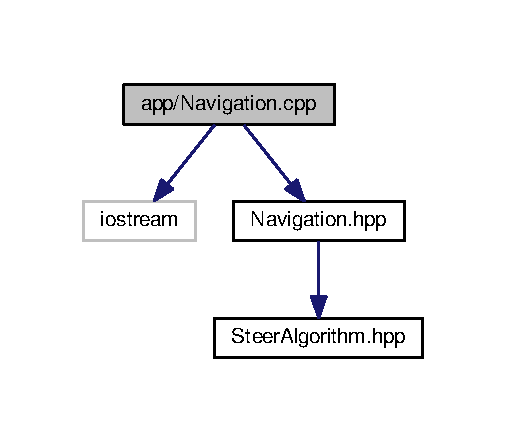
\includegraphics[width=350pt]{_navigation_8cpp__incl}
\end{center}
\end{figure}


\subsection{Detailed Description}
Mid Term Project. 

\begin{DoxyCopyright}{Copyright}
M\+IT License, Copyright © 2019 Raj Shinde
\end{DoxyCopyright}
\begin{DoxyAuthor}{Author}
Sprint-\/1 Raj Shinde-\/ driver and Prasheel Renkuntla-\/ navigator 

Sprint-\/2 Prasheel Renkuntla-\/ driver and Raj Shinde-\/ navigator 
\end{DoxyAuthor}
\begin{DoxyDate}{Date}
10/10/2019 
\end{DoxyDate}
\begin{DoxyVersion}{Version}
6.\+0 
\end{DoxyVersion}
\hypertarget{_steer_algorithm_8cpp_Implements}{}\subsection{Ackermann on P\+I\+D control}\label{_steer_algorithm_8cpp_Implements}

\hypertarget{_steer_algorithm_8cpp}{}\section{app/\+Steer\+Algorithm.cpp File Reference}
\label{_steer_algorithm_8cpp}\index{app/\+Steer\+Algorithm.\+cpp@{app/\+Steer\+Algorithm.\+cpp}}


Mid Term Project.  


{\ttfamily \#include $<$iostream$>$}\\*
{\ttfamily \#include $<$cmath$>$}\\*
{\ttfamily \#include \char`\"{}Steer\+Algorithm.\+hpp\char`\"{}}\\*
Include dependency graph for Steer\+Algorithm.\+cpp\+:
\nopagebreak
\begin{figure}[H]
\begin{center}
\leavevmode
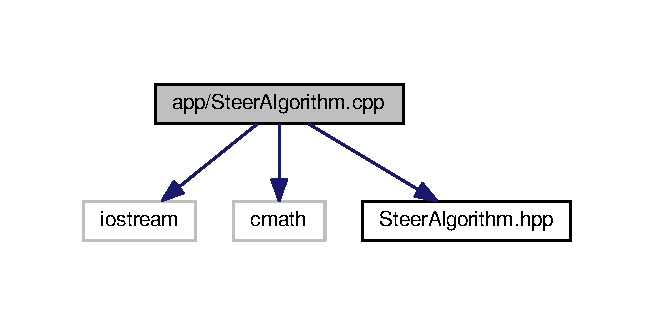
\includegraphics[width=314pt]{_steer_algorithm_8cpp__incl}
\end{center}
\end{figure}


\subsection{Detailed Description}
Mid Term Project. 

\begin{DoxyCopyright}{Copyright}
M\+IT License, Copyright © 2019 Raj Shinde
\end{DoxyCopyright}
\begin{DoxyAuthor}{Author}
Sprint-\/1 Raj Shinde-\/ driver and Prasheel Renkuntla-\/ navigator 

Sprint-\/2 Prasheel Renkuntla-\/ driver and Raj Shinde-\/ navigator 
\end{DoxyAuthor}
\begin{DoxyDate}{Date}
10/10/2019 
\end{DoxyDate}
\begin{DoxyVersion}{Version}
6.\+0 
\end{DoxyVersion}
\hypertarget{_steer_algorithm_8cpp_Implements}{}\subsection{Ackermann on P\+I\+D control}\label{_steer_algorithm_8cpp_Implements}

\hypertarget{gnuplot-iostream_8h}{}\section{include/gnuplot-\/iostream.h File Reference}
\label{gnuplot-iostream_8h}\index{include/gnuplot-\/iostream.\+h@{include/gnuplot-\/iostream.\+h}}
{\ttfamily \#include $<$cstdio$>$}\\*
{\ttfamily \#include $<$fstream$>$}\\*
{\ttfamily \#include $<$iostream$>$}\\*
{\ttfamily \#include $<$sstream$>$}\\*
{\ttfamily \#include $<$stdexcept$>$}\\*
{\ttfamily \#include $<$string$>$}\\*
{\ttfamily \#include $<$utility$>$}\\*
{\ttfamily \#include $<$iomanip$>$}\\*
{\ttfamily \#include $<$vector$>$}\\*
{\ttfamily \#include $<$complex$>$}\\*
{\ttfamily \#include $<$cstdlib$>$}\\*
{\ttfamily \#include $<$cmath$>$}\\*
{\ttfamily \#include $<$boost/iostreams/device/file\+\_\+descriptor.\+hpp$>$}\\*
{\ttfamily \#include $<$boost/iostreams/stream.\+hpp$>$}\\*
{\ttfamily \#include $<$boost/version.\+hpp$>$}\\*
{\ttfamily \#include $<$boost/utility.\+hpp$>$}\\*
{\ttfamily \#include $<$boost/tuple/tuple.\+hpp$>$}\\*
{\ttfamily \#include $<$boost/mpl/bool.\+hpp$>$}\\*
{\ttfamily \#include $<$boost/cstdint.\+hpp$>$}\\*
\subsection*{Classes}
\begin{DoxyCompactItemize}
\item 
struct \hyperlink{structgnuplotio_1_1dont__treat__as__stl__container}{gnuplotio\+::dont\+\_\+treat\+\_\+as\+\_\+stl\+\_\+container$<$ T $>$}
\item 
struct \hyperlink{structgnuplotio_1_1is__like__stl__container}{gnuplotio\+::is\+\_\+like\+\_\+stl\+\_\+container$<$ T $>$}
\item 
struct \hyperlink{structgnuplotio_1_1is__boost__tuple__nulltype}{gnuplotio\+::is\+\_\+boost\+\_\+tuple\+\_\+nulltype$<$ T $>$}
\item 
struct \hyperlink{structgnuplotio_1_1is__boost__tuple__nulltype_3_01boost_1_1tuples_1_1null__type_01_4}{gnuplotio\+::is\+\_\+boost\+\_\+tuple\+\_\+nulltype$<$ boost\+::tuples\+::null\+\_\+type $>$}
\item 
struct \hyperlink{structgnuplotio_1_1is__boost__tuple}{gnuplotio\+::is\+\_\+boost\+\_\+tuple$<$ T $>$}
\item 
class \hyperlink{classgnuplotio_1_1_gnuplot_feedback}{gnuplotio\+::\+Gnuplot\+Feedback}
\item 
struct \hyperlink{structgnuplotio_1_1_text_sender}{gnuplotio\+::\+Text\+Sender$<$ T, Enable $>$}
\item 
struct \hyperlink{structgnuplotio_1_1_binary_sender}{gnuplotio\+::\+Binary\+Sender$<$ T, Enable $>$}
\item 
struct \hyperlink{structgnuplotio_1_1_flat_binary_sender}{gnuplotio\+::\+Flat\+Binary\+Sender$<$ T $>$}
\item 
struct \hyperlink{structgnuplotio_1_1_binfmt_sender}{gnuplotio\+::\+Binfmt\+Sender$<$ T, Enable $>$}
\item 
struct \hyperlink{structgnuplotio_1_1_binfmt_sender_3_01float_01_4}{gnuplotio\+::\+Binfmt\+Sender$<$ float $>$}
\item 
struct \hyperlink{structgnuplotio_1_1_binfmt_sender_3_01double_01_4}{gnuplotio\+::\+Binfmt\+Sender$<$ double $>$}
\item 
struct \hyperlink{structgnuplotio_1_1_binfmt_sender_3_01boost_1_1int8__t_01_4}{gnuplotio\+::\+Binfmt\+Sender$<$ boost\+::int8\+\_\+t $>$}
\item 
struct \hyperlink{structgnuplotio_1_1_binfmt_sender_3_01boost_1_1uint8__t_01_4}{gnuplotio\+::\+Binfmt\+Sender$<$ boost\+::uint8\+\_\+t $>$}
\item 
struct \hyperlink{structgnuplotio_1_1_binfmt_sender_3_01boost_1_1int16__t_01_4}{gnuplotio\+::\+Binfmt\+Sender$<$ boost\+::int16\+\_\+t $>$}
\item 
struct \hyperlink{structgnuplotio_1_1_binfmt_sender_3_01boost_1_1uint16__t_01_4}{gnuplotio\+::\+Binfmt\+Sender$<$ boost\+::uint16\+\_\+t $>$}
\item 
struct \hyperlink{structgnuplotio_1_1_binfmt_sender_3_01boost_1_1int32__t_01_4}{gnuplotio\+::\+Binfmt\+Sender$<$ boost\+::int32\+\_\+t $>$}
\item 
struct \hyperlink{structgnuplotio_1_1_binfmt_sender_3_01boost_1_1uint32__t_01_4}{gnuplotio\+::\+Binfmt\+Sender$<$ boost\+::uint32\+\_\+t $>$}
\item 
struct \hyperlink{structgnuplotio_1_1_binfmt_sender_3_01boost_1_1int64__t_01_4}{gnuplotio\+::\+Binfmt\+Sender$<$ boost\+::int64\+\_\+t $>$}
\item 
struct \hyperlink{structgnuplotio_1_1_binfmt_sender_3_01boost_1_1uint64__t_01_4}{gnuplotio\+::\+Binfmt\+Sender$<$ boost\+::uint64\+\_\+t $>$}
\item 
struct \hyperlink{structgnuplotio_1_1_binary_sender_3_01float_01_4}{gnuplotio\+::\+Binary\+Sender$<$ float $>$}
\item 
struct \hyperlink{structgnuplotio_1_1_binary_sender_3_01double_01_4}{gnuplotio\+::\+Binary\+Sender$<$ double $>$}
\item 
struct \hyperlink{structgnuplotio_1_1_binary_sender_3_01boost_1_1int8__t_01_4}{gnuplotio\+::\+Binary\+Sender$<$ boost\+::int8\+\_\+t $>$}
\item 
struct \hyperlink{structgnuplotio_1_1_binary_sender_3_01boost_1_1uint8__t_01_4}{gnuplotio\+::\+Binary\+Sender$<$ boost\+::uint8\+\_\+t $>$}
\item 
struct \hyperlink{structgnuplotio_1_1_binary_sender_3_01boost_1_1int16__t_01_4}{gnuplotio\+::\+Binary\+Sender$<$ boost\+::int16\+\_\+t $>$}
\item 
struct \hyperlink{structgnuplotio_1_1_binary_sender_3_01boost_1_1uint16__t_01_4}{gnuplotio\+::\+Binary\+Sender$<$ boost\+::uint16\+\_\+t $>$}
\item 
struct \hyperlink{structgnuplotio_1_1_binary_sender_3_01boost_1_1int32__t_01_4}{gnuplotio\+::\+Binary\+Sender$<$ boost\+::int32\+\_\+t $>$}
\item 
struct \hyperlink{structgnuplotio_1_1_binary_sender_3_01boost_1_1uint32__t_01_4}{gnuplotio\+::\+Binary\+Sender$<$ boost\+::uint32\+\_\+t $>$}
\item 
struct \hyperlink{structgnuplotio_1_1_binary_sender_3_01boost_1_1int64__t_01_4}{gnuplotio\+::\+Binary\+Sender$<$ boost\+::int64\+\_\+t $>$}
\item 
struct \hyperlink{structgnuplotio_1_1_binary_sender_3_01boost_1_1uint64__t_01_4}{gnuplotio\+::\+Binary\+Sender$<$ boost\+::uint64\+\_\+t $>$}
\item 
struct \hyperlink{structgnuplotio_1_1_cast_int_text_sender}{gnuplotio\+::\+Cast\+Int\+Text\+Sender$<$ T $>$}
\item 
struct \hyperlink{structgnuplotio_1_1_text_sender_3_01char_01_4}{gnuplotio\+::\+Text\+Sender$<$ char $>$}
\item 
struct \hyperlink{structgnuplotio_1_1_text_sender_3_01signed_01char_01_4}{gnuplotio\+::\+Text\+Sender$<$ signed char $>$}
\item 
struct \hyperlink{structgnuplotio_1_1_text_sender_3_01unsigned_01char_01_4}{gnuplotio\+::\+Text\+Sender$<$ unsigned char $>$}
\item 
struct \hyperlink{structgnuplotio_1_1_float_text_sender}{gnuplotio\+::\+Float\+Text\+Sender$<$ T $>$}
\item 
struct \hyperlink{structgnuplotio_1_1_text_sender_3_01float_01_4}{gnuplotio\+::\+Text\+Sender$<$ float $>$}
\item 
struct \hyperlink{structgnuplotio_1_1_text_sender_3_01double_01_4}{gnuplotio\+::\+Text\+Sender$<$ double $>$}
\item 
struct \hyperlink{structgnuplotio_1_1_text_sender_3_01long_01double_01_4}{gnuplotio\+::\+Text\+Sender$<$ long double $>$}
\item 
struct \hyperlink{structgnuplotio_1_1_text_sender_3_01std_1_1pair_3_01_t_00_01_u_01_4_01_4}{gnuplotio\+::\+Text\+Sender$<$ std\+::pair$<$ T, U $>$ $>$}
\item 
struct \hyperlink{structgnuplotio_1_1_binfmt_sender_3_01std_1_1pair_3_01_t_00_01_u_01_4_01_4}{gnuplotio\+::\+Binfmt\+Sender$<$ std\+::pair$<$ T, U $>$ $>$}
\item 
struct \hyperlink{structgnuplotio_1_1_binary_sender_3_01std_1_1pair_3_01_t_00_01_u_01_4_01_4}{gnuplotio\+::\+Binary\+Sender$<$ std\+::pair$<$ T, U $>$ $>$}
\item 
struct \hyperlink{structgnuplotio_1_1_text_sender_3_01std_1_1complex_3_01_t_01_4_01_4}{gnuplotio\+::\+Text\+Sender$<$ std\+::complex$<$ T $>$ $>$}
\item 
struct \hyperlink{structgnuplotio_1_1_binfmt_sender_3_01std_1_1complex_3_01_t_01_4_01_4}{gnuplotio\+::\+Binfmt\+Sender$<$ std\+::complex$<$ T $>$ $>$}
\item 
struct \hyperlink{structgnuplotio_1_1_binary_sender_3_01std_1_1complex_3_01_t_01_4_01_4}{gnuplotio\+::\+Binary\+Sender$<$ std\+::complex$<$ T $>$ $>$}
\item 
struct \hyperlink{structgnuplotio_1_1_text_sender_3_01_t_00_01typename_01boost_1_1enable__if_3_01boost_1_1mpl_1_1ad1ac3a3da167856c52be6ae54ba2c114}{gnuplotio\+::\+Text\+Sender$<$ T, typename boost\+::enable\+\_\+if$<$ boost\+::mpl\+::and\+\_\+$<$ is\+\_\+boost\+\_\+tuple$<$ T $>$, boost\+::mpl\+::not\+\_\+$<$ is\+\_\+boost\+\_\+tuple\+\_\+nulltype$<$ typename T\+::tail\+\_\+type $>$ $>$ $>$ $>$\+::type $>$}
\item 
struct \hyperlink{structgnuplotio_1_1_text_sender_3_01_t_00_01typename_01boost_1_1enable__if_3_01boost_1_1mpl_1_1ab6d6864cc1b3ed233c9f15134694f953}{gnuplotio\+::\+Text\+Sender$<$ T, typename boost\+::enable\+\_\+if$<$ boost\+::mpl\+::and\+\_\+$<$ is\+\_\+boost\+\_\+tuple$<$ T $>$, is\+\_\+boost\+\_\+tuple\+\_\+nulltype$<$ typename T\+::tail\+\_\+type $>$ $>$ $>$\+::type $>$}
\item 
struct \hyperlink{structgnuplotio_1_1_binfmt_sender_3_01_t_00_01typename_01boost_1_1enable__if_3_01boost_1_1mpl_1_e9270e5cb86823566a0af3940aa51061}{gnuplotio\+::\+Binfmt\+Sender$<$ T, typename boost\+::enable\+\_\+if$<$ boost\+::mpl\+::and\+\_\+$<$ is\+\_\+boost\+\_\+tuple$<$ T $>$, boost\+::mpl\+::not\+\_\+$<$ is\+\_\+boost\+\_\+tuple\+\_\+nulltype$<$ typename T\+::tail\+\_\+type $>$ $>$ $>$ $>$\+::type $>$}
\item 
struct \hyperlink{structgnuplotio_1_1_binfmt_sender_3_01_t_00_01typename_01boost_1_1enable__if_3_01boost_1_1mpl_1_8c86f170c2e2969f5519817e5c367132}{gnuplotio\+::\+Binfmt\+Sender$<$ T, typename boost\+::enable\+\_\+if$<$ boost\+::mpl\+::and\+\_\+$<$ is\+\_\+boost\+\_\+tuple$<$ T $>$, is\+\_\+boost\+\_\+tuple\+\_\+nulltype$<$ typename T\+::tail\+\_\+type $>$ $>$ $>$\+::type $>$}
\item 
struct \hyperlink{structgnuplotio_1_1_binary_sender_3_01_t_00_01typename_01boost_1_1enable__if_3_01boost_1_1mpl_1_916ff7a758aa0b8917fd3b30ff275f06}{gnuplotio\+::\+Binary\+Sender$<$ T, typename boost\+::enable\+\_\+if$<$ boost\+::mpl\+::and\+\_\+$<$ is\+\_\+boost\+\_\+tuple$<$ T $>$, boost\+::mpl\+::not\+\_\+$<$ is\+\_\+boost\+\_\+tuple\+\_\+nulltype$<$ typename T\+::tail\+\_\+type $>$ $>$ $>$ $>$\+::type $>$}
\item 
struct \hyperlink{structgnuplotio_1_1_binary_sender_3_01_t_00_01typename_01boost_1_1enable__if_3_01boost_1_1mpl_1_29e1098ca8b7afc20f2ca0bc2e79506a}{gnuplotio\+::\+Binary\+Sender$<$ T, typename boost\+::enable\+\_\+if$<$ boost\+::mpl\+::and\+\_\+$<$ is\+\_\+boost\+\_\+tuple$<$ T $>$, is\+\_\+boost\+\_\+tuple\+\_\+nulltype$<$ typename T\+::tail\+\_\+type $>$ $>$ $>$\+::type $>$}
\item 
struct \hyperlink{structgnuplotio_1_1_error___was_not_container}{gnuplotio\+::\+Error\+\_\+\+Was\+Not\+Container}
\item 
struct \hyperlink{structgnuplotio_1_1_error___inappropriate_deref}{gnuplotio\+::\+Error\+\_\+\+Inappropriate\+Deref}
\item 
class \hyperlink{classgnuplotio_1_1_array_traits}{gnuplotio\+::\+Array\+Traits$<$ T, Enable $>$}
\item 
class \hyperlink{classgnuplotio_1_1_array_traits_defaults}{gnuplotio\+::\+Array\+Traits\+Defaults$<$ V $>$}
\item 
class \hyperlink{classgnuplotio_1_1_array_traits_3_01_t_01_6_01_4}{gnuplotio\+::\+Array\+Traits$<$ T \& $>$}
\item 
class \hyperlink{classgnuplotio_1_1_iterator_range}{gnuplotio\+::\+Iterator\+Range$<$ T\+I, T\+V $>$}
\item 
class \hyperlink{classgnuplotio_1_1_array_traits_3_01_t_00_01typename_01boost_1_1enable__if_3_01is__like__stl__co9e1736bbd08cd58c6993ab613a998887}{gnuplotio\+::\+Array\+Traits$<$ T, typename boost\+::enable\+\_\+if$<$ is\+\_\+like\+\_\+stl\+\_\+container$<$ T $>$ $>$\+::type $>$}
\item 
class \hyperlink{classgnuplotio_1_1_array_traits_3_01_t[_n]_4}{gnuplotio\+::\+Array\+Traits$<$ T\mbox{[}\+N\mbox{]}$>$}
\item 
class \hyperlink{classgnuplotio_1_1_pair_of_range}{gnuplotio\+::\+Pair\+Of\+Range$<$ R\+T, R\+U $>$}
\item 
class \hyperlink{classgnuplotio_1_1_array_traits_3_01std_1_1pair_3_01_t_00_01_u_01_4_01_4}{gnuplotio\+::\+Array\+Traits$<$ std\+::pair$<$ T, U $>$ $>$}
\item 
class \hyperlink{classgnuplotio_1_1_array_traits_3_01_t_00_01typename_01boost_1_1enable__if_3_01boost_1_1mpl_1_1a8de3a8fe198d85f7f5d28b9a2f5bf229}{gnuplotio\+::\+Array\+Traits$<$ T, typename boost\+::enable\+\_\+if$<$ boost\+::mpl\+::and\+\_\+$<$ is\+\_\+boost\+\_\+tuple$<$ T $>$, boost\+::mpl\+::not\+\_\+$<$ is\+\_\+boost\+\_\+tuple\+\_\+nulltype$<$ typename T\+::tail\+\_\+type $>$ $>$ $>$ $>$\+::type $>$}
\item 
class \hyperlink{classgnuplotio_1_1_array_traits_3_01_t_00_01typename_01boost_1_1enable__if_3_01boost_1_1mpl_1_1ad3fa8e75dccbaae12a06d17831678a88}{gnuplotio\+::\+Array\+Traits$<$ T, typename boost\+::enable\+\_\+if$<$ boost\+::mpl\+::and\+\_\+$<$ is\+\_\+boost\+\_\+tuple$<$ T $>$, is\+\_\+boost\+\_\+tuple\+\_\+nulltype$<$ typename T\+::tail\+\_\+type $>$ $>$ $>$\+::type $>$}
\item 
class \hyperlink{classgnuplotio_1_1_vec_of_range}{gnuplotio\+::\+Vec\+Of\+Range$<$ R\+T $>$}
\item 
class \hyperlink{classgnuplotio_1_1plotting__empty__container}{gnuplotio\+::plotting\+\_\+empty\+\_\+container}
\item 
struct \hyperlink{structgnuplotio_1_1_mode_text}{gnuplotio\+::\+Mode\+Text}
\item 
struct \hyperlink{structgnuplotio_1_1_mode_binary}{gnuplotio\+::\+Mode\+Binary}
\item 
struct \hyperlink{structgnuplotio_1_1_mode_binfmt}{gnuplotio\+::\+Mode\+Binfmt}
\item 
struct \hyperlink{structgnuplotio_1_1_mode_size}{gnuplotio\+::\+Mode\+Size}
\item 
struct \hyperlink{structgnuplotio_1_1_col_unwrap_no}{gnuplotio\+::\+Col\+Unwrap\+No}
\item 
struct \hyperlink{structgnuplotio_1_1_col_unwrap_yes}{gnuplotio\+::\+Col\+Unwrap\+Yes}
\item 
struct \hyperlink{structgnuplotio_1_1_mode1_d}{gnuplotio\+::\+Mode1D}
\item 
struct \hyperlink{structgnuplotio_1_1_mode2_d}{gnuplotio\+::\+Mode2D}
\item 
struct \hyperlink{structgnuplotio_1_1_mode1_d_unwrap}{gnuplotio\+::\+Mode1\+D\+Unwrap}
\item 
struct \hyperlink{structgnuplotio_1_1_mode2_d_unwrap}{gnuplotio\+::\+Mode2\+D\+Unwrap}
\item 
struct \hyperlink{structgnuplotio_1_1_mode_auto}{gnuplotio\+::\+Mode\+Auto}
\item 
struct \hyperlink{structgnuplotio_1_1_mode_auto_decoder}{gnuplotio\+::\+Mode\+Auto\+Decoder$<$ T, Enable $>$}
\item 
struct \hyperlink{structgnuplotio_1_1_mode_auto_decoder_3_01_t_00_01typename_01boost_1_1enable__if__c_3_01_07_arraea646779afc1e35efaeffcebe81e18a0}{gnuplotio\+::type$<$ T $>$}
\item 
struct \hyperlink{structgnuplotio_1_1_mode_auto_decoder_3_01_t_00_01typename_01boost_1_1enable__if__c_3_01_07_arra33ab7f3325313485a7f29355d9a819fc}{gnuplotio\+::type$<$ T $>$}
\item 
struct \hyperlink{structgnuplotio_1_1_mode_auto_decoder_3_01_t_00_01typename_01boost_1_1enable__if__c_3_01_07_arra8faa7fb46cef74a29a23f22c000e4a99}{gnuplotio\+::type$<$ T $>$}
\item 
struct \hyperlink{structgnuplotio_1_1_file_handle_wrapper}{gnuplotio\+::\+File\+Handle\+Wrapper}
\item 
class \hyperlink{classgnuplotio_1_1_gnuplot}{gnuplotio\+::\+Gnuplot}
\end{DoxyCompactItemize}
\subsection*{Namespaces}
\begin{DoxyCompactItemize}
\item 
 \hyperlink{namespacegnuplotio}{gnuplotio}
\end{DoxyCompactItemize}
\subsection*{Macros}
\begin{DoxyCompactItemize}
\item 
\#define \hyperlink{gnuplot-iostream_8h_ab3ce4a7287aefeb9af2345e08cb2d5c6}{G\+N\+U\+P\+L\+O\+T\+\_\+\+I\+O\+S\+T\+R\+E\+A\+M\+\_\+\+V\+E\+R\+S\+I\+ON}~2
\item 
\#define \hyperlink{gnuplot-iostream_8h_aff01a99842ed9eb01a166d4bf19543c9}{G\+N\+U\+P\+L\+O\+T\+\_\+\+E\+N\+A\+B\+L\+E\+\_\+\+C\+X\+X11}~(\+\_\+\+\_\+cplusplus $>$= 201103)
\item 
\#define \hyperlink{gnuplot-iostream_8h_a763d85d6a998475c41e5bea11e6f0a16}{G\+N\+U\+P\+L\+O\+T\+\_\+\+S\+T\+A\+T\+I\+C\+\_\+\+A\+S\+S\+E\+R\+T\+\_\+\+M\+SG}(cond,  msg)~B\+O\+O\+S\+T\+\_\+\+S\+T\+A\+T\+I\+C\+\_\+\+A\+S\+S\+E\+RT((cond))
\item 
\#define \hyperlink{gnuplot-iostream_8h_aceaee9cbe0b7786c1ee8aa2e8b79ed1a}{G\+N\+U\+P\+L\+O\+T\+\_\+\+D\+E\+P\+R\+E\+C\+A\+TE}(msg)
\item 
\#define \hyperlink{gnuplot-iostream_8h_aed027791e656970e6de95b047dc375b1}{G\+N\+U\+P\+L\+O\+T\+\_\+\+P\+C\+L\+O\+SE}~pclose
\item 
\#define \hyperlink{gnuplot-iostream_8h_a92922430eb3df3ace3b18c75b91a0ab8}{G\+N\+U\+P\+L\+O\+T\+\_\+\+P\+O\+P\+EN}~popen
\item 
\#define \hyperlink{gnuplot-iostream_8h_abcc0f8f4d67f147c013bb33b55dc3a16}{G\+N\+U\+P\+L\+O\+T\+\_\+\+F\+I\+L\+E\+NO}~fileno
\item 
\#define \hyperlink{gnuplot-iostream_8h_ac10f83c29b94951000138a0ab2054956}{G\+N\+U\+P\+L\+O\+T\+\_\+\+I\+S\+N\+AN}~std\+::isnan
\item 
\#define \hyperlink{gnuplot-iostream_8h_aef2d72925bdeb9f505df49edbf7579bf}{G\+N\+U\+P\+L\+O\+T\+\_\+\+M\+S\+V\+C\+\_\+\+W\+A\+R\+N\+I\+N\+G\+\_\+4996\+\_\+\+P\+U\+SH}
\item 
\#define \hyperlink{gnuplot-iostream_8h_a4429193ca854af851cec4220c2d9102e}{G\+N\+U\+P\+L\+O\+T\+\_\+\+M\+S\+V\+C\+\_\+\+W\+A\+R\+N\+I\+N\+G\+\_\+4996\+\_\+\+P\+OP}
\item 
\#define \hyperlink{gnuplot-iostream_8h_afe4b1cc99e87d3bb8bbb07280db4b697}{G\+N\+U\+P\+L\+O\+T\+\_\+\+D\+E\+F\+A\+U\+L\+T\+\_\+\+C\+O\+M\+M\+A\+ND}~\char`\"{}gnuplot -\/persist\char`\"{}
\end{DoxyCompactItemize}
\subsection*{Functions}
\begin{DoxyCompactItemize}
\item 
{\footnotesize template$<$typename T $>$ }\\Vec\+Of\+Range$<$ typename Array\+Traits$<$ T $>$\+::range\+\_\+type\+::subiter\+\_\+type $>$ \hyperlink{namespacegnuplotio_a64984827dd8debb9098ad1afdde8e409}{gnuplotio\+::get\+\_\+columns\+\_\+range} (const T \&arg)
\item 
{\footnotesize template$<$typename T $>$ }\\void \hyperlink{namespacegnuplotio_a55ff2f9abaa4b3e1c64a8f730f791b33}{gnuplotio\+::send\+\_\+scalar} (std\+::ostream \&stream, const T \&arg, Mode\+Text)
\item 
{\footnotesize template$<$typename T $>$ }\\void \hyperlink{namespacegnuplotio_a05022d6e136d8ed89a2bef0f61443332}{gnuplotio\+::send\+\_\+scalar} (std\+::ostream \&stream, const T \&arg, Mode\+Binary)
\item 
{\footnotesize template$<$typename T $>$ }\\void \hyperlink{namespacegnuplotio_a926e0935a02d83735da2c34cfbad133f}{gnuplotio\+::send\+\_\+scalar} (std\+::ostream \&stream, const T \&, Mode\+Binfmt)
\item 
{\footnotesize template$<$typename T , typename Print\+Mode $>$ }\\boost\+::disable\+\_\+if\+\_\+c$<$ T\+::is\+\_\+container $>$\+::type \hyperlink{namespacegnuplotio_a66d64f716e539dc233f8183b4ce71c09}{gnuplotio\+::deref\+\_\+and\+\_\+print} (std\+::ostream \&stream, const T \&arg, Print\+Mode)
\item 
{\footnotesize template$<$typename T , typename Print\+Mode $>$ }\\boost\+::enable\+\_\+if\+\_\+c$<$ T\+::is\+\_\+container $>$\+::type \hyperlink{namespacegnuplotio_a8c6b699dd18c419d597a008b74eda41a}{gnuplotio\+::deref\+\_\+and\+\_\+print} (std\+::ostream \&stream, const T \&arg, Print\+Mode)
\item 
{\footnotesize template$<$typename T , typename U , typename Print\+Mode $>$ }\\void \hyperlink{namespacegnuplotio_acd0cb4bd9679f0b75bac15c8afcc10e6}{gnuplotio\+::deref\+\_\+and\+\_\+print} (std\+::ostream \&stream, const Pair\+Of\+Range$<$ T, U $>$ \&arg, Print\+Mode)
\item 
{\footnotesize template$<$typename T , typename Print\+Mode $>$ }\\void \hyperlink{namespacegnuplotio_ae768911c8adb77bfc080d5e4561573e6}{gnuplotio\+::deref\+\_\+and\+\_\+print} (std\+::ostream \&stream, const Vec\+Of\+Range$<$ T $>$ \&arg, Print\+Mode)
\item 
{\footnotesize template$<$size\+\_\+t Depth, typename T , typename Print\+Mode $>$ }\\boost\+::enable\+\_\+if\+\_\+c$<$(Depth==1)\&\&!Print\+Mode\+::is\+\_\+size $>$\+::type \hyperlink{namespacegnuplotio_a631368ab4e255d2a5d563a41895f2edc}{gnuplotio\+::print\+\_\+block} (std\+::ostream \&stream, T \&arg, Print\+Mode)
\item 
{\footnotesize template$<$size\+\_\+t Depth, typename T , typename Print\+Mode $>$ }\\boost\+::enable\+\_\+if\+\_\+c$<$(Depth $>$1)\&\&!Print\+Mode\+::is\+\_\+size $>$\+::type \hyperlink{namespacegnuplotio_a753a3551f418723c022be60c12379025}{gnuplotio\+::print\+\_\+block} (std\+::ostream \&stream, T \&arg, Print\+Mode)
\item 
{\footnotesize template$<$typename T $>$ }\\size\+\_\+t \hyperlink{namespacegnuplotio_abb416b68686102ba84a2cb53c96b64e9}{gnuplotio\+::get\+\_\+range\+\_\+size} (const T \&arg)
\item 
{\footnotesize template$<$size\+\_\+t Depth, typename T , typename Print\+Mode $>$ }\\boost\+::enable\+\_\+if\+\_\+c$<$(Depth==1)\&\&Print\+Mode\+::is\+\_\+size $>$\+::type \hyperlink{namespacegnuplotio_ae470a0908ac5f51527ff76ecbc1616d1}{gnuplotio\+::print\+\_\+block} (std\+::ostream \&stream, T \&arg, Print\+Mode)
\item 
{\footnotesize template$<$size\+\_\+t Depth, typename T , typename Print\+Mode $>$ }\\boost\+::enable\+\_\+if\+\_\+c$<$(Depth $>$1)\&\&Print\+Mode\+::is\+\_\+size $>$\+::type \hyperlink{namespacegnuplotio_a94e97ca55dc1e5142dcc4457a5e1dd2d}{gnuplotio\+::print\+\_\+block} (std\+::ostream \&stream, T \&arg, Print\+Mode)
\item 
{\footnotesize template$<$size\+\_\+t Depth, typename T , typename Print\+Mode $>$ }\\void \hyperlink{namespacegnuplotio_aef147f3d42f3f2c89cc4c895b8494150}{gnuplotio\+::handle\+\_\+colunwrap\+\_\+tag} (std\+::ostream \&stream, const T \&arg, Col\+Unwrap\+No, Print\+Mode)
\item 
{\footnotesize template$<$size\+\_\+t Depth, typename T , typename Print\+Mode $>$ }\\void \hyperlink{namespacegnuplotio_a3b8981d3f39de8a058b5f18484f06c3c}{gnuplotio\+::handle\+\_\+colunwrap\+\_\+tag} (std\+::ostream \&stream, const T \&arg, Col\+Unwrap\+Yes, Print\+Mode)
\item 
{\footnotesize template$<$typename T , typename Print\+Mode $>$ }\\void \hyperlink{namespacegnuplotio_af809657552a53c3b17f0400a5c210a7f}{gnuplotio\+::handle\+\_\+organization\+\_\+tag} (std\+::ostream \&stream, const T \&arg, Mode1D, Print\+Mode)
\item 
{\footnotesize template$<$typename T , typename Print\+Mode $>$ }\\void \hyperlink{namespacegnuplotio_a1310221abf0551a805d4482f0612317b}{gnuplotio\+::handle\+\_\+organization\+\_\+tag} (std\+::ostream \&stream, const T \&arg, Mode2D, Print\+Mode)
\item 
{\footnotesize template$<$typename T , typename Print\+Mode $>$ }\\void \hyperlink{namespacegnuplotio_a99e6125b97bc2ca4241f6275d83f05d4}{gnuplotio\+::handle\+\_\+organization\+\_\+tag} (std\+::ostream \&stream, const T \&arg, Mode1\+D\+Unwrap, Print\+Mode)
\item 
{\footnotesize template$<$typename T , typename Print\+Mode $>$ }\\void \hyperlink{namespacegnuplotio_a9d2cee7a7f2ed9748a0f135b206836d3}{gnuplotio\+::handle\+\_\+organization\+\_\+tag} (std\+::ostream \&stream, const T \&arg, Mode2\+D\+Unwrap, Print\+Mode)
\item 
{\footnotesize template$<$typename T , typename Print\+Mode $>$ }\\void \hyperlink{namespacegnuplotio_affc9cb6a9b6e5630523f0dbf8acdfcc2}{gnuplotio\+::handle\+\_\+organization\+\_\+tag} (std\+::ostream \&stream, const T \&arg, Mode\+Auto, Print\+Mode)
\item 
{\footnotesize template$<$typename T , typename Organization\+Mode , typename Print\+Mode $>$ }\\void \hyperlink{namespacegnuplotio_a1e452d861932700749421ce103ef8d48}{gnuplotio\+::top\+\_\+level\+\_\+array\+\_\+sender} (std\+::ostream \&stream, const T \&arg, Organization\+Mode, Print\+Mode)
\end{DoxyCompactItemize}


\subsection{Macro Definition Documentation}
\index{gnuplot-\/iostream.\+h@{gnuplot-\/iostream.\+h}!G\+N\+U\+P\+L\+O\+T\+\_\+\+D\+E\+F\+A\+U\+L\+T\+\_\+\+C\+O\+M\+M\+A\+ND@{G\+N\+U\+P\+L\+O\+T\+\_\+\+D\+E\+F\+A\+U\+L\+T\+\_\+\+C\+O\+M\+M\+A\+ND}}
\index{G\+N\+U\+P\+L\+O\+T\+\_\+\+D\+E\+F\+A\+U\+L\+T\+\_\+\+C\+O\+M\+M\+A\+ND@{G\+N\+U\+P\+L\+O\+T\+\_\+\+D\+E\+F\+A\+U\+L\+T\+\_\+\+C\+O\+M\+M\+A\+ND}!gnuplot-\/iostream.\+h@{gnuplot-\/iostream.\+h}}
\subsubsection[{\texorpdfstring{G\+N\+U\+P\+L\+O\+T\+\_\+\+D\+E\+F\+A\+U\+L\+T\+\_\+\+C\+O\+M\+M\+A\+ND}{GNUPLOT_DEFAULT_COMMAND}}]{\setlength{\rightskip}{0pt plus 5cm}\#define G\+N\+U\+P\+L\+O\+T\+\_\+\+D\+E\+F\+A\+U\+L\+T\+\_\+\+C\+O\+M\+M\+A\+ND~\char`\"{}gnuplot -\/persist\char`\"{}}\hypertarget{gnuplot-iostream_8h_afe4b1cc99e87d3bb8bbb07280db4b697}{}\label{gnuplot-iostream_8h_afe4b1cc99e87d3bb8bbb07280db4b697}


Definition at line 164 of file gnuplot-\/iostream.\+h.

\index{gnuplot-\/iostream.\+h@{gnuplot-\/iostream.\+h}!G\+N\+U\+P\+L\+O\+T\+\_\+\+D\+E\+P\+R\+E\+C\+A\+TE@{G\+N\+U\+P\+L\+O\+T\+\_\+\+D\+E\+P\+R\+E\+C\+A\+TE}}
\index{G\+N\+U\+P\+L\+O\+T\+\_\+\+D\+E\+P\+R\+E\+C\+A\+TE@{G\+N\+U\+P\+L\+O\+T\+\_\+\+D\+E\+P\+R\+E\+C\+A\+TE}!gnuplot-\/iostream.\+h@{gnuplot-\/iostream.\+h}}
\subsubsection[{\texorpdfstring{G\+N\+U\+P\+L\+O\+T\+\_\+\+D\+E\+P\+R\+E\+C\+A\+TE}{GNUPLOT_DEPRECATE}}]{\setlength{\rightskip}{0pt plus 5cm}\#define G\+N\+U\+P\+L\+O\+T\+\_\+\+D\+E\+P\+R\+E\+C\+A\+TE(
\begin{DoxyParamCaption}
\item[{}]{msg}
\end{DoxyParamCaption}
)}\hypertarget{gnuplot-iostream_8h_aceaee9cbe0b7786c1ee8aa2e8b79ed1a}{}\label{gnuplot-iostream_8h_aceaee9cbe0b7786c1ee8aa2e8b79ed1a}


Definition at line 117 of file gnuplot-\/iostream.\+h.

\index{gnuplot-\/iostream.\+h@{gnuplot-\/iostream.\+h}!G\+N\+U\+P\+L\+O\+T\+\_\+\+E\+N\+A\+B\+L\+E\+\_\+\+C\+X\+X11@{G\+N\+U\+P\+L\+O\+T\+\_\+\+E\+N\+A\+B\+L\+E\+\_\+\+C\+X\+X11}}
\index{G\+N\+U\+P\+L\+O\+T\+\_\+\+E\+N\+A\+B\+L\+E\+\_\+\+C\+X\+X11@{G\+N\+U\+P\+L\+O\+T\+\_\+\+E\+N\+A\+B\+L\+E\+\_\+\+C\+X\+X11}!gnuplot-\/iostream.\+h@{gnuplot-\/iostream.\+h}}
\subsubsection[{\texorpdfstring{G\+N\+U\+P\+L\+O\+T\+\_\+\+E\+N\+A\+B\+L\+E\+\_\+\+C\+X\+X11}{GNUPLOT_ENABLE_CXX11}}]{\setlength{\rightskip}{0pt plus 5cm}\#define G\+N\+U\+P\+L\+O\+T\+\_\+\+E\+N\+A\+B\+L\+E\+\_\+\+C\+X\+X11~(\+\_\+\+\_\+cplusplus $>$= 201103)}\hypertarget{gnuplot-iostream_8h_aff01a99842ed9eb01a166d4bf19543c9}{}\label{gnuplot-iostream_8h_aff01a99842ed9eb01a166d4bf19543c9}


Definition at line 47 of file gnuplot-\/iostream.\+h.

\index{gnuplot-\/iostream.\+h@{gnuplot-\/iostream.\+h}!G\+N\+U\+P\+L\+O\+T\+\_\+\+F\+I\+L\+E\+NO@{G\+N\+U\+P\+L\+O\+T\+\_\+\+F\+I\+L\+E\+NO}}
\index{G\+N\+U\+P\+L\+O\+T\+\_\+\+F\+I\+L\+E\+NO@{G\+N\+U\+P\+L\+O\+T\+\_\+\+F\+I\+L\+E\+NO}!gnuplot-\/iostream.\+h@{gnuplot-\/iostream.\+h}}
\subsubsection[{\texorpdfstring{G\+N\+U\+P\+L\+O\+T\+\_\+\+F\+I\+L\+E\+NO}{GNUPLOT_FILENO}}]{\setlength{\rightskip}{0pt plus 5cm}\#define G\+N\+U\+P\+L\+O\+T\+\_\+\+F\+I\+L\+E\+NO~fileno}\hypertarget{gnuplot-iostream_8h_abcc0f8f4d67f147c013bb33b55dc3a16}{}\label{gnuplot-iostream_8h_abcc0f8f4d67f147c013bb33b55dc3a16}


Definition at line 129 of file gnuplot-\/iostream.\+h.

\index{gnuplot-\/iostream.\+h@{gnuplot-\/iostream.\+h}!G\+N\+U\+P\+L\+O\+T\+\_\+\+I\+O\+S\+T\+R\+E\+A\+M\+\_\+\+V\+E\+R\+S\+I\+ON@{G\+N\+U\+P\+L\+O\+T\+\_\+\+I\+O\+S\+T\+R\+E\+A\+M\+\_\+\+V\+E\+R\+S\+I\+ON}}
\index{G\+N\+U\+P\+L\+O\+T\+\_\+\+I\+O\+S\+T\+R\+E\+A\+M\+\_\+\+V\+E\+R\+S\+I\+ON@{G\+N\+U\+P\+L\+O\+T\+\_\+\+I\+O\+S\+T\+R\+E\+A\+M\+\_\+\+V\+E\+R\+S\+I\+ON}!gnuplot-\/iostream.\+h@{gnuplot-\/iostream.\+h}}
\subsubsection[{\texorpdfstring{G\+N\+U\+P\+L\+O\+T\+\_\+\+I\+O\+S\+T\+R\+E\+A\+M\+\_\+\+V\+E\+R\+S\+I\+ON}{GNUPLOT_IOSTREAM_VERSION}}]{\setlength{\rightskip}{0pt plus 5cm}\#define G\+N\+U\+P\+L\+O\+T\+\_\+\+I\+O\+S\+T\+R\+E\+A\+M\+\_\+\+V\+E\+R\+S\+I\+ON~2}\hypertarget{gnuplot-iostream_8h_ab3ce4a7287aefeb9af2345e08cb2d5c6}{}\label{gnuplot-iostream_8h_ab3ce4a7287aefeb9af2345e08cb2d5c6}


Definition at line 44 of file gnuplot-\/iostream.\+h.

\index{gnuplot-\/iostream.\+h@{gnuplot-\/iostream.\+h}!G\+N\+U\+P\+L\+O\+T\+\_\+\+I\+S\+N\+AN@{G\+N\+U\+P\+L\+O\+T\+\_\+\+I\+S\+N\+AN}}
\index{G\+N\+U\+P\+L\+O\+T\+\_\+\+I\+S\+N\+AN@{G\+N\+U\+P\+L\+O\+T\+\_\+\+I\+S\+N\+AN}!gnuplot-\/iostream.\+h@{gnuplot-\/iostream.\+h}}
\subsubsection[{\texorpdfstring{G\+N\+U\+P\+L\+O\+T\+\_\+\+I\+S\+N\+AN}{GNUPLOT_ISNAN}}]{\setlength{\rightskip}{0pt plus 5cm}\#define G\+N\+U\+P\+L\+O\+T\+\_\+\+I\+S\+N\+AN~std\+::isnan}\hypertarget{gnuplot-iostream_8h_ac10f83c29b94951000138a0ab2054956}{}\label{gnuplot-iostream_8h_ac10f83c29b94951000138a0ab2054956}


Definition at line 137 of file gnuplot-\/iostream.\+h.

\index{gnuplot-\/iostream.\+h@{gnuplot-\/iostream.\+h}!G\+N\+U\+P\+L\+O\+T\+\_\+\+M\+S\+V\+C\+\_\+\+W\+A\+R\+N\+I\+N\+G\+\_\+4996\+\_\+\+P\+OP@{G\+N\+U\+P\+L\+O\+T\+\_\+\+M\+S\+V\+C\+\_\+\+W\+A\+R\+N\+I\+N\+G\+\_\+4996\+\_\+\+P\+OP}}
\index{G\+N\+U\+P\+L\+O\+T\+\_\+\+M\+S\+V\+C\+\_\+\+W\+A\+R\+N\+I\+N\+G\+\_\+4996\+\_\+\+P\+OP@{G\+N\+U\+P\+L\+O\+T\+\_\+\+M\+S\+V\+C\+\_\+\+W\+A\+R\+N\+I\+N\+G\+\_\+4996\+\_\+\+P\+OP}!gnuplot-\/iostream.\+h@{gnuplot-\/iostream.\+h}}
\subsubsection[{\texorpdfstring{G\+N\+U\+P\+L\+O\+T\+\_\+\+M\+S\+V\+C\+\_\+\+W\+A\+R\+N\+I\+N\+G\+\_\+4996\+\_\+\+P\+OP}{GNUPLOT_MSVC_WARNING_4996_POP}}]{\setlength{\rightskip}{0pt plus 5cm}\#define G\+N\+U\+P\+L\+O\+T\+\_\+\+M\+S\+V\+C\+\_\+\+W\+A\+R\+N\+I\+N\+G\+\_\+4996\+\_\+\+P\+OP}\hypertarget{gnuplot-iostream_8h_a4429193ca854af851cec4220c2d9102e}{}\label{gnuplot-iostream_8h_a4429193ca854af851cec4220c2d9102e}


Definition at line 152 of file gnuplot-\/iostream.\+h.

\index{gnuplot-\/iostream.\+h@{gnuplot-\/iostream.\+h}!G\+N\+U\+P\+L\+O\+T\+\_\+\+M\+S\+V\+C\+\_\+\+W\+A\+R\+N\+I\+N\+G\+\_\+4996\+\_\+\+P\+U\+SH@{G\+N\+U\+P\+L\+O\+T\+\_\+\+M\+S\+V\+C\+\_\+\+W\+A\+R\+N\+I\+N\+G\+\_\+4996\+\_\+\+P\+U\+SH}}
\index{G\+N\+U\+P\+L\+O\+T\+\_\+\+M\+S\+V\+C\+\_\+\+W\+A\+R\+N\+I\+N\+G\+\_\+4996\+\_\+\+P\+U\+SH@{G\+N\+U\+P\+L\+O\+T\+\_\+\+M\+S\+V\+C\+\_\+\+W\+A\+R\+N\+I\+N\+G\+\_\+4996\+\_\+\+P\+U\+SH}!gnuplot-\/iostream.\+h@{gnuplot-\/iostream.\+h}}
\subsubsection[{\texorpdfstring{G\+N\+U\+P\+L\+O\+T\+\_\+\+M\+S\+V\+C\+\_\+\+W\+A\+R\+N\+I\+N\+G\+\_\+4996\+\_\+\+P\+U\+SH}{GNUPLOT_MSVC_WARNING_4996_PUSH}}]{\setlength{\rightskip}{0pt plus 5cm}\#define G\+N\+U\+P\+L\+O\+T\+\_\+\+M\+S\+V\+C\+\_\+\+W\+A\+R\+N\+I\+N\+G\+\_\+4996\+\_\+\+P\+U\+SH}\hypertarget{gnuplot-iostream_8h_aef2d72925bdeb9f505df49edbf7579bf}{}\label{gnuplot-iostream_8h_aef2d72925bdeb9f505df49edbf7579bf}


Definition at line 151 of file gnuplot-\/iostream.\+h.

\index{gnuplot-\/iostream.\+h@{gnuplot-\/iostream.\+h}!G\+N\+U\+P\+L\+O\+T\+\_\+\+P\+C\+L\+O\+SE@{G\+N\+U\+P\+L\+O\+T\+\_\+\+P\+C\+L\+O\+SE}}
\index{G\+N\+U\+P\+L\+O\+T\+\_\+\+P\+C\+L\+O\+SE@{G\+N\+U\+P\+L\+O\+T\+\_\+\+P\+C\+L\+O\+SE}!gnuplot-\/iostream.\+h@{gnuplot-\/iostream.\+h}}
\subsubsection[{\texorpdfstring{G\+N\+U\+P\+L\+O\+T\+\_\+\+P\+C\+L\+O\+SE}{GNUPLOT_PCLOSE}}]{\setlength{\rightskip}{0pt plus 5cm}\#define G\+N\+U\+P\+L\+O\+T\+\_\+\+P\+C\+L\+O\+SE~pclose}\hypertarget{gnuplot-iostream_8h_aed027791e656970e6de95b047dc375b1}{}\label{gnuplot-iostream_8h_aed027791e656970e6de95b047dc375b1}


Definition at line 127 of file gnuplot-\/iostream.\+h.

\index{gnuplot-\/iostream.\+h@{gnuplot-\/iostream.\+h}!G\+N\+U\+P\+L\+O\+T\+\_\+\+P\+O\+P\+EN@{G\+N\+U\+P\+L\+O\+T\+\_\+\+P\+O\+P\+EN}}
\index{G\+N\+U\+P\+L\+O\+T\+\_\+\+P\+O\+P\+EN@{G\+N\+U\+P\+L\+O\+T\+\_\+\+P\+O\+P\+EN}!gnuplot-\/iostream.\+h@{gnuplot-\/iostream.\+h}}
\subsubsection[{\texorpdfstring{G\+N\+U\+P\+L\+O\+T\+\_\+\+P\+O\+P\+EN}{GNUPLOT_POPEN}}]{\setlength{\rightskip}{0pt plus 5cm}\#define G\+N\+U\+P\+L\+O\+T\+\_\+\+P\+O\+P\+EN~popen}\hypertarget{gnuplot-iostream_8h_a92922430eb3df3ace3b18c75b91a0ab8}{}\label{gnuplot-iostream_8h_a92922430eb3df3ace3b18c75b91a0ab8}


Definition at line 128 of file gnuplot-\/iostream.\+h.

\index{gnuplot-\/iostream.\+h@{gnuplot-\/iostream.\+h}!G\+N\+U\+P\+L\+O\+T\+\_\+\+S\+T\+A\+T\+I\+C\+\_\+\+A\+S\+S\+E\+R\+T\+\_\+\+M\+SG@{G\+N\+U\+P\+L\+O\+T\+\_\+\+S\+T\+A\+T\+I\+C\+\_\+\+A\+S\+S\+E\+R\+T\+\_\+\+M\+SG}}
\index{G\+N\+U\+P\+L\+O\+T\+\_\+\+S\+T\+A\+T\+I\+C\+\_\+\+A\+S\+S\+E\+R\+T\+\_\+\+M\+SG@{G\+N\+U\+P\+L\+O\+T\+\_\+\+S\+T\+A\+T\+I\+C\+\_\+\+A\+S\+S\+E\+R\+T\+\_\+\+M\+SG}!gnuplot-\/iostream.\+h@{gnuplot-\/iostream.\+h}}
\subsubsection[{\texorpdfstring{G\+N\+U\+P\+L\+O\+T\+\_\+\+S\+T\+A\+T\+I\+C\+\_\+\+A\+S\+S\+E\+R\+T\+\_\+\+M\+SG}{GNUPLOT_STATIC_ASSERT_MSG}}]{\setlength{\rightskip}{0pt plus 5cm}\#define G\+N\+U\+P\+L\+O\+T\+\_\+\+S\+T\+A\+T\+I\+C\+\_\+\+A\+S\+S\+E\+R\+T\+\_\+\+M\+SG(
\begin{DoxyParamCaption}
\item[{}]{cond, }
\item[{}]{msg}
\end{DoxyParamCaption}
)~B\+O\+O\+S\+T\+\_\+\+S\+T\+A\+T\+I\+C\+\_\+\+A\+S\+S\+E\+RT((cond))}\hypertarget{gnuplot-iostream_8h_a763d85d6a998475c41e5bea11e6f0a16}{}\label{gnuplot-iostream_8h_a763d85d6a998475c41e5bea11e6f0a16}


Definition at line 104 of file gnuplot-\/iostream.\+h.


\hypertarget{_navigation_8hpp}{}\section{include/\+Navigation.hpp File Reference}
\label{_navigation_8hpp}\index{include/\+Navigation.\+hpp@{include/\+Navigation.\+hpp}}


Mid Term Project.  


{\ttfamily \#include \char`\"{}Steer\+Algorithm.\+hpp\char`\"{}}\\*
{\ttfamily \#include $<$vector$>$}\\*
\subsection*{Classes}
\begin{DoxyCompactItemize}
\item 
class \hyperlink{class_navigation}{Navigation}
\begin{DoxyCompactList}\small\item\em Class \hyperlink{class_navigation}{Navigation} Contains the methods of Pid Algorithm. \end{DoxyCompactList}\end{DoxyCompactItemize}


\subsection{Detailed Description}
Mid Term Project. 

\begin{DoxyCopyright}{Copyright}
M\+IT License, Copyright © 2019 Raj Shinde
\end{DoxyCopyright}
\begin{DoxyAuthor}{Author}
Sprint-\/1 Raj Shinde-\/ driver and Prasheel Renkuntla-\/ navigator 

Sprint-\/2 Prasheel Renkuntla-\/ driver and Raj Shinde-\/ navigator 
\end{DoxyAuthor}
\begin{DoxyDate}{Date}
10/10/2019 
\end{DoxyDate}
\begin{DoxyVersion}{Version}
6.\+0 
\end{DoxyVersion}
\hypertarget{_navigation_8hpp_Header}{}\subsection{file for Navigation through P\+I\+D control}\label{_navigation_8hpp_Header}

\hypertarget{_steer_algorithm_8hpp}{}\section{include/\+Steer\+Algorithm.hpp File Reference}
\label{_steer_algorithm_8hpp}\index{include/\+Steer\+Algorithm.\+hpp@{include/\+Steer\+Algorithm.\+hpp}}


Mid Term Project.  


This graph shows which files directly or indirectly include this file\+:
\nopagebreak
\begin{figure}[H]
\begin{center}
\leavevmode
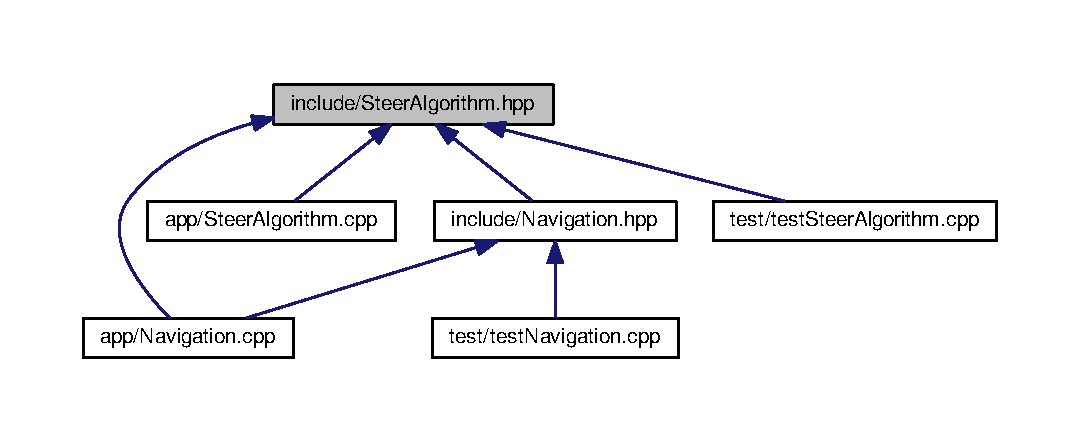
\includegraphics[width=350pt]{_steer_algorithm_8hpp__dep__incl}
\end{center}
\end{figure}
\subsection*{Classes}
\begin{DoxyCompactItemize}
\item 
class \hyperlink{class_steer_algorithm}{Steer\+Algorithm}
\begin{DoxyCompactList}\small\item\em Class \hyperlink{class_steer_algorithm}{Steer\+Algorithm} contains the methods of the Steering Algorithm. \end{DoxyCompactList}\end{DoxyCompactItemize}


\subsection{Detailed Description}
Mid Term Project. 

\begin{DoxyCopyright}{Copyright}
M\+IT License, Copyright © 2019 Raj Shinde
\end{DoxyCopyright}
\begin{DoxyAuthor}{Author}
Sprint-\/1 Raj Shinde-\/ driver and Prasheel Renkuntla-\/ navigator 

Sprint-\/2 Prasheel Renkuntla-\/ driver and Raj Shinde-\/ navigator 
\end{DoxyAuthor}
\begin{DoxyDate}{Date}
10/10/2019 
\end{DoxyDate}
\begin{DoxyVersion}{Version}
6.\+0 
\end{DoxyVersion}
\hypertarget{_steer_algorithm_8hpp_Ackermann}{}\subsection{Steering Control Header file}\label{_steer_algorithm_8hpp_Ackermann}

\hypertarget{_r_e_a_d_m_e_8md}{}\section{R\+E\+A\+D\+M\+E.\+md File Reference}
\label{_r_e_a_d_m_e_8md}\index{R\+E\+A\+D\+M\+E.\+md@{R\+E\+A\+D\+M\+E.\+md}}

\hypertarget{mock_navigation_8cpp}{}\section{test/mock\+Navigation.cpp File Reference}
\label{mock_navigation_8cpp}\index{test/mock\+Navigation.\+cpp@{test/mock\+Navigation.\+cpp}}


Mid Term Project.  


{\ttfamily \#include $<$gtest/gtest.\+h$>$}\\*
{\ttfamily \#include $<$gmock/gmock.\+h$>$}\\*
{\ttfamily \#include $<$vector$>$}\\*
{\ttfamily \#include \char`\"{}iostream\char`\"{}}\\*
{\ttfamily \#include \char`\"{}Navigation.\+hpp\char`\"{}}\\*
\subsection*{Classes}
\begin{DoxyCompactItemize}
\item 
class \hyperlink{class_mock_navigation}{Mock\+Navigation}
\begin{DoxyCompactList}\small\item\em Mock Class \hyperlink{class_navigation}{Navigation} To implement google mock. \end{DoxyCompactList}\end{DoxyCompactItemize}
\subsection*{Functions}
\begin{DoxyCompactItemize}
\item 
\hyperlink{mock_navigation_8cpp_afa4f1fdcc49d8cae82093e455233f67e}{T\+E\+ST} (\hyperlink{class_mock_navigation}{Mock\+Navigation}, check\+Kp)
\item 
\hyperlink{mock_navigation_8cpp_ab9c056b9285f5adb19253a96b7c24a40}{T\+E\+ST} (\hyperlink{class_mock_navigation}{Mock\+Navigation}, check\+Ki)
\item 
\hyperlink{mock_navigation_8cpp_ae07284692a8f21de4325275c3a18a9bf}{T\+E\+ST} (\hyperlink{class_mock_navigation}{Mock\+Navigation}, check\+Kd)
\item 
\hyperlink{mock_navigation_8cpp_a6be533ac83530d2c6b5c0e38f1186fea}{T\+E\+ST} (\hyperlink{class_mock_navigation}{Mock\+Navigation}, check\+P\+ID)
\item 
\hyperlink{mock_navigation_8cpp_a4f7cc4afa8a4ed97f080e692640ba531}{T\+E\+ST} (\hyperlink{class_mock_navigation}{Mock\+Navigation}, check\+Navigation)
\end{DoxyCompactItemize}


\subsection{Detailed Description}
Mid Term Project. 

\begin{DoxyCopyright}{Copyright}
M\+IT License, Copyright © 2019 Raj Shinde
\end{DoxyCopyright}
\begin{DoxyAuthor}{Author}
Prasheel Renkuntla 
\end{DoxyAuthor}
\begin{DoxyDate}{Date}
11/22/2019 
\end{DoxyDate}
\begin{DoxyVersion}{Version}
7.\+0 
\end{DoxyVersion}
\hypertarget{test_steer_algorithm_8cpp_Tests}{}\subsection{all files in module with gmock}\label{test_steer_algorithm_8cpp_Tests}


\subsection{Function Documentation}
\index{mock\+Navigation.\+cpp@{mock\+Navigation.\+cpp}!T\+E\+ST@{T\+E\+ST}}
\index{T\+E\+ST@{T\+E\+ST}!mock\+Navigation.\+cpp@{mock\+Navigation.\+cpp}}
\subsubsection[{\texorpdfstring{T\+E\+S\+T(\+Mock\+Navigation, check\+Kp)}{TEST(MockNavigation, checkKp)}}]{\setlength{\rightskip}{0pt plus 5cm}T\+E\+ST (
\begin{DoxyParamCaption}
\item[{{\bf Mock\+Navigation}}]{, }
\item[{check\+Kp}]{}
\end{DoxyParamCaption}
)}\hypertarget{mock_navigation_8cpp_afa4f1fdcc49d8cae82093e455233f67e}{}\label{mock_navigation_8cpp_afa4f1fdcc49d8cae82093e455233f67e}


Definition at line 98 of file mock\+Navigation.\+cpp.

\index{mock\+Navigation.\+cpp@{mock\+Navigation.\+cpp}!T\+E\+ST@{T\+E\+ST}}
\index{T\+E\+ST@{T\+E\+ST}!mock\+Navigation.\+cpp@{mock\+Navigation.\+cpp}}
\subsubsection[{\texorpdfstring{T\+E\+S\+T(\+Mock\+Navigation, check\+Ki)}{TEST(MockNavigation, checkKi)}}]{\setlength{\rightskip}{0pt plus 5cm}T\+E\+ST (
\begin{DoxyParamCaption}
\item[{{\bf Mock\+Navigation}}]{, }
\item[{check\+Ki}]{}
\end{DoxyParamCaption}
)}\hypertarget{mock_navigation_8cpp_ab9c056b9285f5adb19253a96b7c24a40}{}\label{mock_navigation_8cpp_ab9c056b9285f5adb19253a96b7c24a40}


Definition at line 112 of file mock\+Navigation.\+cpp.

\index{mock\+Navigation.\+cpp@{mock\+Navigation.\+cpp}!T\+E\+ST@{T\+E\+ST}}
\index{T\+E\+ST@{T\+E\+ST}!mock\+Navigation.\+cpp@{mock\+Navigation.\+cpp}}
\subsubsection[{\texorpdfstring{T\+E\+S\+T(\+Mock\+Navigation, check\+Kd)}{TEST(MockNavigation, checkKd)}}]{\setlength{\rightskip}{0pt plus 5cm}T\+E\+ST (
\begin{DoxyParamCaption}
\item[{{\bf Mock\+Navigation}}]{, }
\item[{check\+Kd}]{}
\end{DoxyParamCaption}
)}\hypertarget{mock_navigation_8cpp_ae07284692a8f21de4325275c3a18a9bf}{}\label{mock_navigation_8cpp_ae07284692a8f21de4325275c3a18a9bf}


Definition at line 126 of file mock\+Navigation.\+cpp.

\index{mock\+Navigation.\+cpp@{mock\+Navigation.\+cpp}!T\+E\+ST@{T\+E\+ST}}
\index{T\+E\+ST@{T\+E\+ST}!mock\+Navigation.\+cpp@{mock\+Navigation.\+cpp}}
\subsubsection[{\texorpdfstring{T\+E\+S\+T(\+Mock\+Navigation, check\+P\+I\+D)}{TEST(MockNavigation, checkPID)}}]{\setlength{\rightskip}{0pt plus 5cm}T\+E\+ST (
\begin{DoxyParamCaption}
\item[{{\bf Mock\+Navigation}}]{, }
\item[{check\+P\+ID}]{}
\end{DoxyParamCaption}
)}\hypertarget{mock_navigation_8cpp_a6be533ac83530d2c6b5c0e38f1186fea}{}\label{mock_navigation_8cpp_a6be533ac83530d2c6b5c0e38f1186fea}


Definition at line 141 of file mock\+Navigation.\+cpp.

\index{mock\+Navigation.\+cpp@{mock\+Navigation.\+cpp}!T\+E\+ST@{T\+E\+ST}}
\index{T\+E\+ST@{T\+E\+ST}!mock\+Navigation.\+cpp@{mock\+Navigation.\+cpp}}
\subsubsection[{\texorpdfstring{T\+E\+S\+T(\+Mock\+Navigation, check\+Navigation)}{TEST(MockNavigation, checkNavigation)}}]{\setlength{\rightskip}{0pt plus 5cm}T\+E\+ST (
\begin{DoxyParamCaption}
\item[{{\bf Mock\+Navigation}}]{, }
\item[{check\+Navigation}]{}
\end{DoxyParamCaption}
)}\hypertarget{mock_navigation_8cpp_a4f7cc4afa8a4ed97f080e692640ba531}{}\label{mock_navigation_8cpp_a4f7cc4afa8a4ed97f080e692640ba531}


Definition at line 153 of file mock\+Navigation.\+cpp.


\hypertarget{test_navigation_8cpp}{}\section{test/test\+Navigation.cpp File Reference}
\label{test_navigation_8cpp}\index{test/test\+Navigation.\+cpp@{test/test\+Navigation.\+cpp}}


Mid Term Project.  


{\ttfamily \#include $<$gtest/gtest.\+h$>$}\\*
{\ttfamily \#include $<$cstdlib$>$}\\*
{\ttfamily \#include $<$memory$>$}\\*
{\ttfamily \#include \char`\"{}Navigation.\+hpp\char`\"{}}\\*
\subsection*{Functions}
\begin{DoxyCompactItemize}
\item 
\hyperlink{test_navigation_8cpp_a093604a7433c91e9a41a6c486ff843b3}{T\+E\+ST} (\hyperlink{class_navigation}{Navigation}, test\+Set\+Pid)
\item 
\hyperlink{test_navigation_8cpp_a5c632ae16e5ba30ae35d75900430e15a}{T\+E\+ST} (\hyperlink{class_navigation}{Navigation}, test\+Get\+Pid)
\item 
\hyperlink{test_navigation_8cpp_ae18ffeef30aacd9eb6294f8eb5460d80}{T\+E\+ST} (\hyperlink{class_navigation}{Navigation}, test\+P\+ID)
\item 
\hyperlink{test_navigation_8cpp_acc7325d4d1f9e57e7d887a7af00c04b8}{T\+E\+ST} (\hyperlink{class_navigation}{Navigation}, test\+Convergence)
\item 
\hyperlink{test_navigation_8cpp_ad175cd43f79b49368e38d6706c97f1c0}{T\+E\+ST} (\hyperlink{class_navigation}{Navigation}, test\+Velocity\+Plot)
\item 
\hyperlink{test_navigation_8cpp_a3bdb2deb2b979e58079008d0e44cf8ae}{T\+E\+ST} (\hyperlink{class_navigation}{Navigation}, test\+Steer\+Angle\+Plot)
\end{DoxyCompactItemize}


\subsection{Detailed Description}
Mid Term Project. 

\begin{DoxyCopyright}{Copyright}
M\+IT License, Copyright © 2019 Raj Shinde
\end{DoxyCopyright}
\begin{DoxyAuthor}{Author}
Sprint-\/1 Raj Shinde-\/ driver and Prasheel Renkuntla-\/ navigator 

Sprint-\/2 Prasheel Renkuntla-\/ driver and Raj Shinde-\/ navigator 

Gmock-\/ Prasheel Renkuntla 
\end{DoxyAuthor}
\begin{DoxyDate}{Date}
11/22/2019 
\end{DoxyDate}
\begin{DoxyVersion}{Version}
7.\+0 
\end{DoxyVersion}
\hypertarget{test_steer_algorithm_8cpp_Tests}{}\subsection{all files in module with gmock}\label{test_steer_algorithm_8cpp_Tests}


\subsection{Function Documentation}
\index{test\+Navigation.\+cpp@{test\+Navigation.\+cpp}!T\+E\+ST@{T\+E\+ST}}
\index{T\+E\+ST@{T\+E\+ST}!test\+Navigation.\+cpp@{test\+Navigation.\+cpp}}
\subsubsection[{\texorpdfstring{T\+E\+S\+T(\+Navigation, test\+Set\+Pid)}{TEST(Navigation, testSetPid)}}]{\setlength{\rightskip}{0pt plus 5cm}T\+E\+ST (
\begin{DoxyParamCaption}
\item[{{\bf Navigation}}]{, }
\item[{test\+Set\+Pid}]{}
\end{DoxyParamCaption}
)}\hypertarget{test_navigation_8cpp_a093604a7433c91e9a41a6c486ff843b3}{}\label{test_navigation_8cpp_a093604a7433c91e9a41a6c486ff843b3}


Definition at line 50 of file test\+Navigation.\+cpp.

\index{test\+Navigation.\+cpp@{test\+Navigation.\+cpp}!T\+E\+ST@{T\+E\+ST}}
\index{T\+E\+ST@{T\+E\+ST}!test\+Navigation.\+cpp@{test\+Navigation.\+cpp}}
\subsubsection[{\texorpdfstring{T\+E\+S\+T(\+Navigation, test\+Get\+Pid)}{TEST(Navigation, testGetPid)}}]{\setlength{\rightskip}{0pt plus 5cm}T\+E\+ST (
\begin{DoxyParamCaption}
\item[{{\bf Navigation}}]{, }
\item[{test\+Get\+Pid}]{}
\end{DoxyParamCaption}
)}\hypertarget{test_navigation_8cpp_a5c632ae16e5ba30ae35d75900430e15a}{}\label{test_navigation_8cpp_a5c632ae16e5ba30ae35d75900430e15a}


Definition at line 63 of file test\+Navigation.\+cpp.

\index{test\+Navigation.\+cpp@{test\+Navigation.\+cpp}!T\+E\+ST@{T\+E\+ST}}
\index{T\+E\+ST@{T\+E\+ST}!test\+Navigation.\+cpp@{test\+Navigation.\+cpp}}
\subsubsection[{\texorpdfstring{T\+E\+S\+T(\+Navigation, test\+P\+I\+D)}{TEST(Navigation, testPID)}}]{\setlength{\rightskip}{0pt plus 5cm}T\+E\+ST (
\begin{DoxyParamCaption}
\item[{{\bf Navigation}}]{, }
\item[{test\+P\+ID}]{}
\end{DoxyParamCaption}
)}\hypertarget{test_navigation_8cpp_ae18ffeef30aacd9eb6294f8eb5460d80}{}\label{test_navigation_8cpp_ae18ffeef30aacd9eb6294f8eb5460d80}


Definition at line 76 of file test\+Navigation.\+cpp.

\index{test\+Navigation.\+cpp@{test\+Navigation.\+cpp}!T\+E\+ST@{T\+E\+ST}}
\index{T\+E\+ST@{T\+E\+ST}!test\+Navigation.\+cpp@{test\+Navigation.\+cpp}}
\subsubsection[{\texorpdfstring{T\+E\+S\+T(\+Navigation, test\+Convergence)}{TEST(Navigation, testConvergence)}}]{\setlength{\rightskip}{0pt plus 5cm}T\+E\+ST (
\begin{DoxyParamCaption}
\item[{{\bf Navigation}}]{, }
\item[{test\+Convergence}]{}
\end{DoxyParamCaption}
)}\hypertarget{test_navigation_8cpp_acc7325d4d1f9e57e7d887a7af00c04b8}{}\label{test_navigation_8cpp_acc7325d4d1f9e57e7d887a7af00c04b8}


Definition at line 88 of file test\+Navigation.\+cpp.

\index{test\+Navigation.\+cpp@{test\+Navigation.\+cpp}!T\+E\+ST@{T\+E\+ST}}
\index{T\+E\+ST@{T\+E\+ST}!test\+Navigation.\+cpp@{test\+Navigation.\+cpp}}
\subsubsection[{\texorpdfstring{T\+E\+S\+T(\+Navigation, test\+Velocity\+Plot)}{TEST(Navigation, testVelocityPlot)}}]{\setlength{\rightskip}{0pt plus 5cm}T\+E\+ST (
\begin{DoxyParamCaption}
\item[{{\bf Navigation}}]{, }
\item[{test\+Velocity\+Plot}]{}
\end{DoxyParamCaption}
)}\hypertarget{test_navigation_8cpp_ad175cd43f79b49368e38d6706c97f1c0}{}\label{test_navigation_8cpp_ad175cd43f79b49368e38d6706c97f1c0}


Definition at line 102 of file test\+Navigation.\+cpp.

\index{test\+Navigation.\+cpp@{test\+Navigation.\+cpp}!T\+E\+ST@{T\+E\+ST}}
\index{T\+E\+ST@{T\+E\+ST}!test\+Navigation.\+cpp@{test\+Navigation.\+cpp}}
\subsubsection[{\texorpdfstring{T\+E\+S\+T(\+Navigation, test\+Steer\+Angle\+Plot)}{TEST(Navigation, testSteerAnglePlot)}}]{\setlength{\rightskip}{0pt plus 5cm}T\+E\+ST (
\begin{DoxyParamCaption}
\item[{{\bf Navigation}}]{, }
\item[{test\+Steer\+Angle\+Plot}]{}
\end{DoxyParamCaption}
)}\hypertarget{test_navigation_8cpp_a3bdb2deb2b979e58079008d0e44cf8ae}{}\label{test_navigation_8cpp_a3bdb2deb2b979e58079008d0e44cf8ae}


Definition at line 115 of file test\+Navigation.\+cpp.


\hypertarget{test_steer_algorithm_8cpp}{}\section{test/test\+Steer\+Algorithm.cpp File Reference}
\label{test_steer_algorithm_8cpp}\index{test/test\+Steer\+Algorithm.\+cpp@{test/test\+Steer\+Algorithm.\+cpp}}


Mid Term Project.  


{\ttfamily \#include $<$gtest/gtest.\+h$>$}\\*
{\ttfamily \#include $<$cstdlib$>$}\\*
{\ttfamily \#include $<$memory$>$}\\*
{\ttfamily \#include \char`\"{}Steer\+Algorithm.\+hpp\char`\"{}}\\*
Include dependency graph for test\+Steer\+Algorithm.\+cpp\+:
\nopagebreak
\begin{figure}[H]
\begin{center}
\leavevmode
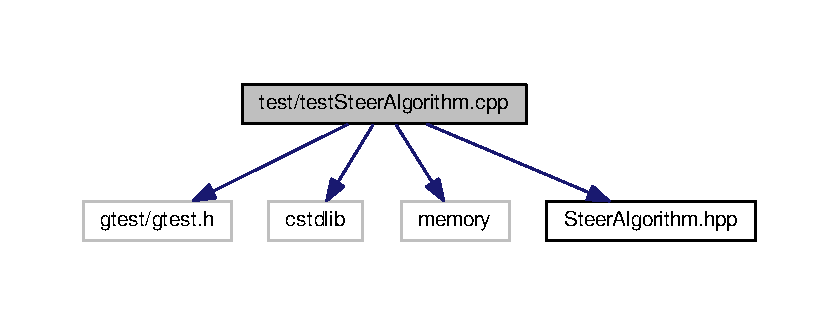
\includegraphics[width=350pt]{test_steer_algorithm_8cpp__incl}
\end{center}
\end{figure}
\subsection*{Functions}
\begin{DoxyCompactItemize}
\item 
\hyperlink{test_steer_algorithm_8cpp_a302ee9fe0ef08a6beaea103c911981ff}{T\+E\+ST} (\hyperlink{class_steer_algorithm}{Steer\+Algorithm}, test\+Corr\+Radius)\hypertarget{test_steer_algorithm_8cpp_a302ee9fe0ef08a6beaea103c911981ff}{}\label{test_steer_algorithm_8cpp_a302ee9fe0ef08a6beaea103c911981ff}

\begin{DoxyCompactList}\small\item\em Tests to check that the set functions works and the value of corr\+Radius in below setlimit. \end{DoxyCompactList}\item 
\hyperlink{test_steer_algorithm_8cpp_ab38a7e56f4e7418febe58d9daf9e4b58}{T\+E\+ST} (\hyperlink{class_steer_algorithm}{Steer\+Algorithm}, testwheel)\hypertarget{test_steer_algorithm_8cpp_ab38a7e56f4e7418febe58d9daf9e4b58}{}\label{test_steer_algorithm_8cpp_ab38a7e56f4e7418febe58d9daf9e4b58}

\begin{DoxyCompactList}\small\item\em Tests to check if the wheel angles get resetted and the Ackeermann kinematic model is is properly implemented. \end{DoxyCompactList}\item 
\hyperlink{test_steer_algorithm_8cpp_a2e8c38dec883b8cfc46adb1e0cedb000}{T\+E\+ST} (\hyperlink{class_steer_algorithm}{Steer\+Algorithm}, test\+Calculations)\hypertarget{test_steer_algorithm_8cpp_a2e8c38dec883b8cfc46adb1e0cedb000}{}\label{test_steer_algorithm_8cpp_a2e8c38dec883b8cfc46adb1e0cedb000}

\begin{DoxyCompactList}\small\item\em Test to check the functions arclength and turn\+Time provide right length and time values. \end{DoxyCompactList}\end{DoxyCompactItemize}


\subsection{Detailed Description}
Mid Term Project. 

\begin{DoxyCopyright}{Copyright}
M\+IT License, Copyright © 2019 Raj Shinde
\end{DoxyCopyright}
\begin{DoxyAuthor}{Author}
Sprint-\/1 Raj Shinde-\/ driver and Prasheel Renkuntla-\/ navigator 

Sprint-\/2 Prasheel Renkuntla-\/ driver and Raj Shinde-\/ navigator 
\end{DoxyAuthor}
\begin{DoxyDate}{Date}
10/10/2019 
\end{DoxyDate}
\begin{DoxyVersion}{Version}
6.\+0 
\end{DoxyVersion}
\hypertarget{test_steer_algorithm_8cpp_Tests}{}\subsection{all files in module}\label{test_steer_algorithm_8cpp_Tests}

%--- End generated contents ---

% Index
\backmatter
\newpage
\phantomsection
\clearemptydoublepage
\addcontentsline{toc}{chapter}{Index}
\printindex

\end{document}
